% Gelfand seminar notes, 1987-88: source pages P001385-P001479.
% Russian diplomatic transcription (AI-made, checked against the scans), cut page by page from the cumulative working reader A4-reader-chapters01-34-complete-first1527-separated-diplomatic-r59.
% \SourcePage{GELFAND-Pnnnnnn}{label} starts a scanned page; the second argument is the number written
% on the page, if any. Editorial notes give the page, a label and the transcriber's remark; \Unclear
% marks a doubtful reading.
\SourcePage{GELFAND-P001385}{1}

\uuline{5/X-87 г.}\qquad \uline{Сем. Гельфанда.}

\uuline{А. Бейлинсон.}\qquad
\uline{Конструктивные пучки} (продолжение).

\uwave{Программа по пучкам.}

1. Пучок, категория пучков.

2. Операции над пучками:

\hspace*{2em}а) Склейки по открытому покрытию

\hspace*{2em}б) Склейка открытого и замкнутого мн-ва

\hspace*{2em}в) Прямые и обратные образы.

3. Локально постоянные пучки.

4. Комбинаторные
[зачёркнуто:
возможно «конструктивные»\textsuperscript{?}]
пучки \(=\) представления упорядоченных множеств.

\Unclear{GELFAND-P001385}{cancelled-upper}{возможно «конструктивные»}
\end{GelfandAdjacentEvidence}
\begin{GelfandAdjacentEvidence}{GELFAND-P001385}{2}



5. Конструктивные пучки.

6. Когомологии с коэффициентами в пучках.

7. Двойственность Пуанкаре--Вердье

Пп. 1--5 см. в предыдущей тетради.

Пучки образуют \uwave{абелеву категорию}.

Пусть \(\mathcal F,G\) --- пучки и дан морфизм
\(\mathcal F\overset{\varphi}{\longrightarrow}G\).

Все морфизмы образуют вект. пр-во (над \(\mathbb C\))

\uline{Определение 1.}

\(\operatorname{Ker}\varphi\subset\mathcal F\)
[Под формулой: подпучок]
\[
(\ker\varphi)(V)=\{a\in\mathcal F(V),\ \varphi(a)=0\}
\]

\(\operatorname{Coker}\varphi\) --- пучок, ассоциированный с предпучком \(C\) вида
\[
C(V)=\operatorname{Coker}\bigl(\varphi:\mathcal F(V)\longrightarrow G(V)\bigr)
\]

\uwave{Построение пучка по предпучку.}

Пусть \(C\) --- предпучок.

Пусть \(V\) --- открытое мн-во, \(V=\bigcup V_\alpha\) и даны
\(a_\alpha\in C(V_\alpha)\), согласованные между собой:
\[
a_\alpha|_{V_\alpha\cap V_\beta}=a_\beta|_{V_\alpha\cap V_\beta}.
\]
Такой набор определяет сечение пучка. Имеется отождествление сечений,
«получ.»
из различных наборов.

\EvidenceBlock{GELFAND-P001385}{lower-gluing}{В рукописи «получ.».}{Запись в рукописи.}
\end{GelfandAdjacentEvidence}
\begin{GelfandAdjacentEvidence}{GELFAND-P001385}{3}



\(C^+\) --- [зачёркнуто:
возможно «пред.»\textsuperscript{?}]
пучок, ассоциированный с \(C\).

\Unclear{GELFAND-P001385}{cancelled-bottom}{возможно «пред.»}
\end{GelfandAdjacentEvidence}



\Needspace{7\baselineskip}
\begin{GelfandAdjacentEvidence}{GELFAND-P001386}{1}
\SourcePage{GELFAND-P001386}{unlabelled}

Имеется отобр. \(C\longrightarrow C^+\), универсальное в след. смысле

\SourceFigure{GELFAND-P001386}{universal-diagram}{%
\begingroup\color{black}\GelfandFitDiagram{\begin{tikzpicture}[x=1cm,y=1cm,>=stealth]
  \node (c) at (0,1.6) {$C$};
  \node (plus) at (2.0,1.6) {$C^+$};
  \node (f) at (1.7,0) {$\mathcal F$};
  \draw[->] (c) -- (plus);
  \draw[->] (c) -- node[below left] {$\forall f$} (f);
  \draw[->,dashed] (plus) -- node[right] {$f^+\!\leftarrow\!\exists!$} (f);
  \draw (f.south east) -- ++(.18,-.16) node[right] {\scriptsize пучок};
\end{tikzpicture}}\endgroup}
\end{GelfandAdjacentEvidence}
\begin{GelfandAdjacentEvidence}{GELFAND-P001386}{2}


\(\forall\) отобр. \(f\colon C\longrightarrow\mathcal F\)
[под \(\mathcal F\): пучок]
\(\exists!\ f^+\colon C^+\longrightarrow\mathcal F\), что коммут. диаграмма

\uline{Упражнение 1.}
[зачёркнуто: «про…»?]
построить \(C^+\).

\Unclear{GELFAND-P001386}{cancelled-exercise}{«про…»?}
\end{GelfandAdjacentEvidence}
\begin{GelfandAdjacentEvidence}{GELFAND-P001386}{3}



Имеются отображения
\[
\operatorname{Ker}\varphi\overset{\alpha}{\longrightarrow}\mathcal F
\overset{\varphi}{\longrightarrow}G
\overset{\beta}{\longrightarrow}\operatorname{Coker}\varphi
\]

\uline{Упражнение 2.}\quad \(\operatorname{Ker}\beta=\operatorname{Coker}\alpha\)

Естеств. образом опред. точная послед. пучков.

\uline{Упражнение 3.}\quad
Послед. \(\mathcal F_1\longrightarrow\mathcal F_2\longrightarrow\mathcal F_3\)
точна \(\Longleftrightarrow\ \forall x\in X\)
послед. \(\mathcal F_{1x}\longrightarrow\mathcal F_{2x}\longrightarrow\mathcal F_{3x}\)
точна.

(Рассм. вложение \(x\overset{i_x}{\longrightarrow}X\), тогда слой
\(\mathcal F_x\) в точке \(x\) имеет вид \(\mathcal F_x=i_x^*\mathcal F\))

\uline{Опред. 2} (\uline{Вялый пучок}.)

Пучок \(\mathcal F\) наз. вялым, если любое его сеч. над откр. мн-вом \(V\) продолж. до сеч. над всем \(X\),
т.е. \(\forall\) откр. \(V\subset X\)
\[
\mathcal F(X)\longrightarrow\mathcal F(V)
\]
есть эпиморфизм.

\SourceFigure{GELFAND-P001386}{path-diagram}{%
\begingroup\color{black}\GelfandFitDiagram{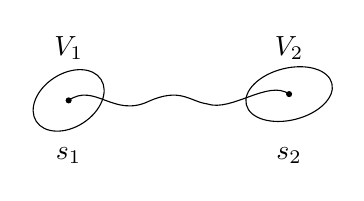
\begin{tikzpicture}[x=1cm,y=1cm]
  \draw[rotate around={33:(0,0)}] (0,0) ellipse (.49 and .34);
  \draw[rotate around={14:(2.8,.08)}] (2.8,.08) ellipse (.56 and .33);
  \draw (0,0) .. controls (.33,.23) and (.57,-.22) .. (1.01,-.015)
    .. controls (1.42,.17) and (1.53,-.01) .. (1.76,-.045)
    .. controls (2.07,-.15) and (2.54,.27) .. (2.8,.08);
  \fill (0,0) circle (1.1pt) (2.8,.08) circle (1.1pt);
  \node at (0,.66) {$V_1$}; \node at (2.8,.66) {$V_2$};
  \node at (0,-.70) {$s_1$}; \node at (2.8,-.70) {$s_2$};
\end{tikzpicture}}\endgroup\par Нижние подписи читаются как \(s_1\), \(s_2\), возможно \(\xi_1\), \(\xi_2\).}
\end{GelfandAdjacentEvidence}


В лок. пост. пучках можно переносить сечения [вставлено над строкой: (вдоль пути)] и по этому такие пучки не явл. \uline{вялыми}.

\uline{Задача 4.}\quad \(\Gamma\) --- 
[вставлено над строкой: конечное] упорядоченное множество; введем топологию
\[
\overline{x}:=\{y:\ y\leq x\}\quad\text{--- замыкание точки }x
\]
а) Пучки на \(\Gamma\) \(=\) представления \(\Gamma\)

б) Описать вялые пучки на \(\Gamma\)


\Needspace{7\baselineskip}
\begin{GelfandAdjacentEvidence}{GELFAND-P001387}{1}
\SourcePage{GELFAND-P001387}{2}

в) Связь с комбинаторными пучками

Пусть на \(X\) есть стратификация, рассм. отображение
\SourceFigure{GELFAND-P001387}{stratum-map}{%
\begingroup\color{black}\GelfandFitDiagram{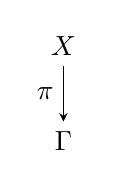
\begin{tikzpicture}[>=stealth]
  \node (space) at (0,1.2) {$X$};
  \node (strata) at (0,0) {$\Gamma$};
  \draw[->] (space) -- node[left] {$\pi$} (strata);
\end{tikzpicture}}\endgroup}
\end{GelfandAdjacentEvidence}
\begin{GelfandAdjacentEvidence}{GELFAND-P001387}{2}

(точке \(x\) --- ее страт)

\(\Gamma\) --- упоряд. мн-во стратов.

[под \(\Gamma\):] Введ. на \(\Gamma\) топ. (Зарисского)

\uline{Утв.}

\uwave{\(\forall\) комбинаторный пучок на \(X\) есть обратный образ}
[зачёркнуто: «пучков»?]
\uwave{пучка на \(\Gamma\)}
(и наоборот)


\Unclear{GELFAND-P001387}{cancelled-pullback}{«пучков»?}
\end{GelfandAdjacentEvidence}
\begin{GelfandAdjacentEvidence}{GELFAND-P001387}{3}

\[
\pi^*\colon\text{пучки на }\Gamma\overset{\sim}{\longrightarrow}
\text{комбинат. пучки на }X.
\]

\uline{Упражнение 5.}\quad а) Пусть
\[
0\longrightarrow\mathcal F_1\longrightarrow\mathcal F_2\longrightarrow
\mathcal F_3\longrightarrow0
\]
--- короткая точная послед. пучков. Тогда послед. сечений
\[
0\longrightarrow\mathcal F_1(X)\longrightarrow\mathcal F_2(X)
\longrightarrow\mathcal F_3(X)
\]
точна.

б) Если \(\mathcal F_1\) --- вялый, то точна послед.
\[
0\longrightarrow\mathcal F_1(X)\longrightarrow\mathcal F_2(X)
\longrightarrow\mathcal F_3(X)\longrightarrow0
\]

\uline{Вялая резольвента пучка.}

\uline{Упражнение 6}\quad Пусть \(\mathcal F\) --- пучок; тогда 1) Его можно вложить в вялый пучок
\(\mathcal F\hookrightarrow G\).

2) Теперь строим по \(\mathcal F\) точную последовательность

\SourceFigure{GELFAND-P001387}{flabby-resolution-diagram}{%
\resizebox{\linewidth}{!}{%
\begingroup\color{black}\GelfandFitDiagram{\begin{tikzpicture}[x=1cm,y=1cm,>=stealth]
  \node (zero) at (0,0) {$0$};
  \node (f) at (.87,0) {$\mathcal F$};
  \node (g0) at (1.9,0) {$G^0$};
  \node (g1) at (3.44,0) {$G^1$};
  \node (g2) at (5.05,0) {$G^2$};
  \node (tail) at (6.09,0) {$\ldots$};
  \node (q0) at (2.56,-.94) {$G^0/\mathcal F$};
  \node (q1) at (4.30,-.94) {$G^1/(G^0/\mathcal F)$};
  \node[right] at (6.29,0) {$,\quad G^i$ --- вялые};
  \draw[->] (zero) -- (f);
  \draw[->] (f) -- (g0);
  \draw[->] (g0) -- (g1);
  \draw[->] (g1) -- (g2);
  \draw[->] (g2) -- (tail);
  \draw[->] (g0.south) -- (q0.north west);
  \draw[->] (q0.north east) to[out=213,in=-97,looseness=1.35] (g1.south);
  \draw[->] (g1.south) -- (q1.north west);
  \draw[->] (q1.north east) to[out=213,in=-97,looseness=1.35] (g2.south);
  \node at (2.55,-1.60) {и т.д.};
\end{tikzpicture}}\endgroup}}
\end{GelfandAdjacentEvidence}


(вялая резольвента)

3) \(\forall\) две вялые резольвенты можно вложить в общую 3-ю.

\uline{Определение 3.}
\[
H^i(X,\mathcal F)=H^i\bigl(0\longrightarrow G^0(X)\longrightarrow
G^1(X)\longrightarrow\ldots\bigr)
\]
(здесь \(0\longrightarrow\mathcal F\longrightarrow G^0\longrightarrow
G^1\longrightarrow\ldots\) --- вялая резольвента \(\mathcal F\))

Справа стоят когомологии комплекса линейных пространств.

\uline{Определение 4.}\quad [зачёркнуто: Двойственный пучок.]
\uwave{Когом. с компактным носителем.}

Предположим, что \(X\) локально компактно. Тогда можно рассм. сечения с компактным носителем:
\(\mathcal F_c(X)\) --- сеч. с комп. носит. на \(X\).


\Needspace{7\baselineskip}
\begin{GelfandAdjacentEvidence}{GELFAND-P001388}{1}
\SourcePage{GELFAND-P001388}{unlabelled}

\[
H_c^i(X,\mathcal F)=H^i\bigl(0\longrightarrow G_c^0(X)\longrightarrow
G_c^1(X)\longrightarrow\ldots\bigr)
\]

\uline{Определение 5.}\quad Двойственный пучок.

Предпучок: \(\mathcal F^*(V)=\mathcal F_c(V)^*\)
(аналог: «распределения», возможно «распределений»\textsuperscript{?})
\Unclear{GELFAND-P001388}{dual-note}{«распределения», возможно «распределений»}
\end{GelfandAdjacentEvidence}


(двойств. пр-во в смысле лин. алгебры)
\[
V_1\subset V_2\ \Rightarrow\ \mathcal F_c(V_1)\longrightarrow\mathcal F_c(V_2)
\quad\text{(вложение)}
\]
и возникает \(\mathcal F^*(V_2)\longrightarrow\mathcal F^*(V_1)\)

\uline{Упражнение 7.}

а) \(\mathcal F^*\) --- пучок, если \(\mathcal F\) вялый.

б) Если \(\mathcal F^*\) --- пучок, то \(\mathcal F^*\)
--- вялый, т.е. \(\forall\underset{\text{откр.}}{V}\subset X\)
отобр. \(\mathcal F^*(X)\longrightarrow\mathcal F^*(V)\) сюръективно


\Needspace{7\baselineskip}
\begin{GelfandAdjacentEvidence}{GELFAND-P001389}{1}
\SourcePage{GELFAND-P001389}{unlabelled}

\uline{12.10.87 г.}\qquad \uline{Сем. Гельфанда.}

Вахтангов велел артистам в принцессе Турандот выходить на сцену в модных одеждах и сразу переодеваться (надевать чалму и т.п.). Сюжеты математики вечны, меняется только язык.

\uline{И. М. Г.}\quad \uline{Об одной комбинаторной гипотезе Дайсона, связ. с полином. коэффициентами}

\uwave{Одна раб. из зеленого толстого сборника по комбинаторике}

Рассматривается
\begin{equation*}
F(x,a)=\prod_{i\ne j}\left(1-\frac{x_j}{x_i}\right)^{a_j},
\qquad a_j\in\mathbb N.
\tag{1}
\end{equation*}
Найти свободный член

Гипотеза Дайсона (1962): ответ
\begin{equation*}
\frac{(a_1+a_2\ldots+a_n)!}{a_1!a_2!\ldots a_n!}
\tag{2}
\end{equation*}

В 1962 даны 2 док-ва J. Math. Phys. (длинные)

В 1970 J. Math. Phys. док-во
\EvidenceBlock{GELFAND-P001389}{author-name}{«Вуда»}{Запись в рукописи.}
\end{GelfandAdjacentEvidence}
\begin{GelfandAdjacentEvidence}{GELFAND-P001389}{2}

в 2 строчки.

\uline{Д-во}\quad Применяя интерполяц. ф-лу Лагранжа ф-и \(f\equiv0\)
\EvidenceBlock{GELFAND-P001389}{interpolation-function}{В рукописи стоит \(f\equiv0\).}{Запись в рукописи.}
\end{GelfandAdjacentEvidence}

и полагая затем \(x=0\), получаем
\begin{equation*}
\sum_j\prod_{i\ne j}\left(1-\frac{x_j}{x_i}\right)^{-1}=1
\tag{3}
\end{equation*}

Умножая на \(F(x,a)\), получаем


\Needspace{7\baselineskip}
\begin{GelfandAdjacentEvidence}{GELFAND-P001390}{1}
\SourcePage{GELFAND-P001390}{unlabelled}

\begin{equation*}
\sum_j F(x,a_1,\ldots,a_{j-1},a_j-1,a_{j+1},\ldots,a_n)=F(x,a)
\tag{4}
\end{equation*}

[зачёркнуто: неразборчивое начало]
\Unclear{GELFAND-P001390}{cancelled-let}{неразборчивое начало}
\end{GelfandAdjacentEvidence}
\begin{GelfandAdjacentEvidence}{GELFAND-P001390}{2}

Пусть \(G(a)\) --- своб. член. Тогда из (4)
\begin{equation*}
G(a)=\sum G(a_1,\ldots,a_{j-1},a_j-1,a_{j+1},\ldots,a_n),
\tag{5}
\end{equation*}
что дает рекуррентную ф-лу.

При \(a_j=0\) получаем
\begin{equation*}
\begin{aligned}
G(a_1,\ldots,a_{j-1},0,a_{j+1},\ldots,a_n)
&=G(a_1,\ldots,a_{j-1},a_{j+1},\ldots,a_n)
\end{aligned}
\tag{6}
\end{equation*}
Кроме того,
\begin{equation*}
G(0)=1
\tag{7}
\end{equation*}
Соотношения (5)--(7) являются достаточными рекуррентными соотношениями, к-рыми всё определяется и получается (2).

\uuline{А. Веселов}

\uline{О геодезических на эллипсоиде и дв-нии на сфере}

По Якоби и другим --- 1982. наблюд. Кноррера: эквивалентность 2-х задач.

[Две колонки, разделённые фигурной линией. Левая колонка.]

1) \((Aq,q)=1\)

геодезические на эллипсоиде

Вейерштрасс нашел в \(\theta\)-ф-ях (1861)

Ур-е геодезич. в натур. параметре:
\begin{equation*}
\ddot q=\lambda Aq
\tag{1}
\end{equation*}
(ускорение \(\sim\) нормали)

[Справа:] (\(\lambda\) --- множитель Лагранжа, нах. из усл. \((Aq,q)=1\))

[Правая колонка.]

2) Другая задача [зачёркнуто:
\(C.\) после инициала фамилия зачёркнута, возможно «Neu…»\textsuperscript{?}]
\Unclear{GELFAND-P001390}{cancelled-neumann}{\(C.\) после инициала фамилия зачёркнута, возможно «Neu…»}
\end{GelfandAdjacentEvidence}
\begin{GelfandAdjacentEvidence}{GELFAND-P001390}{3}

C. Neumann (1859)

Дв-ние с потенц. энергией
\[
U(x)=\frac12(Ax,x)
\]
на сфере \(\lvert x\rvert^2=1\)

Здесь ур-е
\begin{equation*}
x''=-Ax+ux
\tag{\(1'\)}
\end{equation*}
или в координатах
\begin{equation*}
x_i''=-a_i x_i+ux_i
\tag{\(1''\)}
\end{equation*}
[справа зачёркнут знак:
\(q\)? / \(u\)?\textsuperscript{?}]
\Unclear{GELFAND-P001390}{equation-end}{\(q\)? / \(u\)?}
\end{GelfandAdjacentEvidence}
\begin{GelfandAdjacentEvidence}{GELFAND-P001390}{4}


[Ниже колонок.]

Перейдем к другому параметру
\begin{equation*}
q''=-Aq+vq'
\tag{2}
\end{equation*}
(замены явно выписываются,
\(\underset{\substack{\parallel\\\mathrm{const}}}{\lambda}\rightsquigarrow
\underset{\substack{\parallel\\\mathrm{const}}}{v}\))
\Unclear{GELFAND-P001390}{constants-note}{Под \(\lambda\) и \(v\) написано «const», по два коротких штриха над каждой надписью. Значение штрихов неясно.}
\end{GelfandAdjacentEvidence}
\begin{GelfandAdjacentEvidence}{GELFAND-P001390}{5}


и тогда замена
\begin{equation*}
x=\frac{Aq}{\lvert Aq\rvert}\qquad\text{(подст. Гаусса)}
\tag{3}
\end{equation*}
переводит решения зад. 1) в реш. 2) (прямая выкладка)
\EvidenceBlock{GELFAND-P001390}{bijection-note}{В рукописи «прямая выкладка».}{Запись в рукописи.}
\end{GelfandAdjacentEvidence}


(H. Knörrer, 1982)

Ур-е

[Справа:] Введем оператор:
\begin{equation*}
L=-\frac{d^2}{dt^2}+u,\qquad Lx_i=a_i x_i
\tag{4}
\end{equation*}
(\(x_i\) --- соб. ф-я!!)


\Needspace{7\baselineskip}
\SourcePage{GELFAND-P001391}{12}

Слева:
\begin{equation*}
\widetilde L=-\frac{d^2}{dt^2}+v\frac{d}{dt}
\tag{5}
\end{equation*}
(сопряжен к \(L\) с помощью подст. Гаусса или подст. Миуры)

Knörrer пришел через изоморфизм Мозера--Трубовица

\uwave{Рассм. задачу 2)}

Имеются 2 симплектич. формы.

\uline{Задача} (И. М. Г.) Имеется симм. матр. \(A\) и матр. \(K\) ранга 1.
Как по соб. знач. \(A+K\) восстановить \(K\)? (\(A\) фиксировано)

--- это и есть ф-ла Якоби.

\uline{В.}\quad Введем при \(n=2\) новые координаты
\begin{gather*}
M=[\dot x,x],\qquad\text{(момент --- вект. произведение)}\\
p=x
\end{gather*}

\(1^{\circ}\). Скобка Ли--Березина--Кириллова
\begin{gather*}
\{M_i,M_j\}=\varepsilon_{ijk}M_k\\
\{M_i,p_j\}=\varepsilon_{ijk}p_k\\
\{p_i,p_j\}=0
\end{gather*}

Гамильтониан
\[
2H=M^2+(Ap,p)
\]
Тогда
\[
\begin{cases}
\dot M_i=\{M_i,H\}\\
\dot p_i=\{p_i,H\}
\end{cases}
\qquad\text{--- ур-я Неймана}
\]

\uwave{2-я скобка}
\begin{gather*}
\varepsilon_{ijk}a_kM_k=\{M_i,M_j\}\\
\varepsilon_{ijk}a_kp_k=\{M_i,p_j\}\\
\varepsilon_{ijk}M_k=\{p_i,p_j\}
\end{gather*}

Гамильтониан \(F=\frac12p^2\)

\uwave{И. М. Г.}\quad Это совпадает с тем, что рассказывал Арнольд

(см. предыд. тетрадь)

Система гамильтонова и в той и в другой.


\Needspace{7\baselineskip}
\begin{GelfandAdjacentEvidence}{GELFAND-P001392}{1}
\SourcePage{GELFAND-P001392}{unlabelled}

\uuline{А. Бейлинсон.}\quad \uwave{Конструктивные пучки} (продолжение)

Представления частично упоряд. мн-ва \(\Longleftrightarrow\)
[зачёркнуто: возможно «конструктивные»\textsuperscript{?}]
комбинаторные пучки

\Unclear{GELFAND-P001392}{cancelled-equivalence}{возможно «конструктивные»}
\end{GelfandAdjacentEvidence}
\begin{GelfandAdjacentEvidence}{GELFAND-P001392}{2}



\SourceFigure{GELFAND-P001392}{interval-strata}{%
\begingroup\color{black}\GelfandFitDiagram{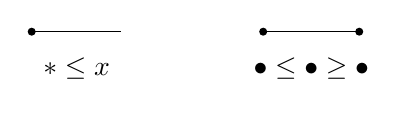
\begin{tikzpicture}[x=1cm,y=1cm]
  \draw (0,0) -- (1.14,0);
  \fill (0,0) circle (1.45pt);
  \draw (2.94,0) -- (4.16,0);
  \fill (2.94,0) circle (1.45pt) (4.16,0) circle (1.45pt);
  \node at (.57,-.47) {$\ast\leq x$};
  \node at (3.55,-.47) {$\bullet\leq\bullet\geq\bullet$};
\end{tikzpicture}}\endgroup}
\end{GelfandAdjacentEvidence}
\begin{GelfandAdjacentEvidence}{GELFAND-P001392}{3}


Комбинаторный пучок --- пучок, постоянный на каждом страте.

\uwave{Гомологическая алгебра.}

\(\mathcal A\) --- абелева категория (например, пучков над данным пр-вом или модулей)

\(C(\mathcal A)\) --- категория комплексов над \(\mathcal A\)

надо знать \uwave{производную категорию} (Verdier, 1961)

Объекты [зачёркнуто:
возможно «из» или знак принадлежности\textsuperscript{?}]
\(C(\mathcal A)\)


\Unclear{GELFAND-P001392}{objects-mark}{возможно «из» или знак принадлежности}
\end{GelfandAdjacentEvidence}
\begin{GelfandAdjacentEvidence}{GELFAND-P001392}{4}

\begin{gather*}
\ldots\longrightarrow X^i\overset{d}{\longrightarrow}X^{i+1}
\overset{d}{\longrightarrow}X^{i+2}\longrightarrow\ldots\\
d^2=0
\end{gather*}
морфизмы --- морфизмы комплексов (наборы морф.
\SourceFigure{GELFAND-P001392}{component-morphism}{%
\begingroup\color{black}\GelfandFitDiagram{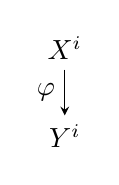
\begin{tikzpicture}[>=stealth]
  \node (x) at (0,1.12) {$X^i$};
  \node (y) at (0,0) {$Y^i$};
  \draw[->] (x) -- node[left] {$\varphi$} (y);
\end{tikzpicture}}\endgroup}
\end{GelfandAdjacentEvidence}
\begin{GelfandAdjacentEvidence}{GELFAND-P001392}{5}

, перестан. с \(d\))

\(C(\mathcal A)\) --- тоже абелева категория

Огранич. комплексы (лишь конечное число \(\ne0\)) \(C^b(\mathcal A)\)

огранич. слева или справа \(C^{\pm}(\mathcal A)\)
\begin{gather*}
C^+(\mathcal A)\text{ --- огр. слева}\\
C^-(\mathcal A)\text{ --- огр. справа}
\end{gather*}

Гомотопическая категория \(K(\mathcal A)\)

объекты \(K(\mathcal A)\) те же, что в \(C(\mathcal A)\),
а морфизмы --- классы эквив. морфизмов \(C(\mathcal A)\) относит. гомотопии.
\[
\operatorname{Hom}_{K(\mathcal A)}(X^\bullet,Y^\bullet)
\]

Морфизм \(X^\bullet\overset{\varphi}{\longrightarrow}Y^\bullet\)
--- это [вставлено над строкой: такой] набор
\(\varphi^i\colon X^i\longrightarrow Y^i\), что коммут. диаграмма:

\SourceFigure{GELFAND-P001392}{homotopy-diagrams}{%
\resizebox{\linewidth}{!}{%
\begingroup\color{black}\GelfandFitDiagram{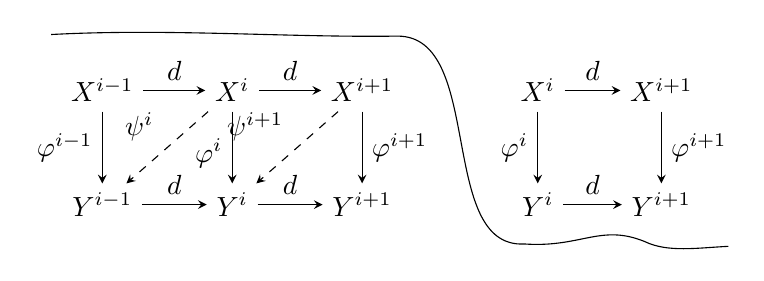
\begin{tikzpicture}[x=1cm,y=1cm,>=stealth]
  \node (xm) at (0,1.45) {$X^{i-1}$};
  \node (x) at (1.65,1.45) {$X^i$};
  \node (xp) at (3.3,1.45) {$X^{i+1}$};
  \node (ym) at (0,0) {$Y^{i-1}$};
  \node (y) at (1.65,0) {$Y^i$};
  \node (yp) at (3.3,0) {$Y^{i+1}$};
  \node (rx) at (5.53,1.45) {$X^i$};
  \node (rxp) at (7.10,1.45) {$X^{i+1}$};
  \node (ry) at (5.53,0) {$Y^i$};
  \node (ryp) at (7.10,0) {$Y^{i+1}$};
  \draw[->] (xm) -- node[above] {$d$} (x);
  \draw[->] (x) -- node[above] {$d$} (xp);
  \draw[->] (ym) -- node[above] {$d$} (y);
  \draw[->] (y) -- node[above] {$d$} (yp);
  \draw[->] (xm) -- node[left] {$\varphi^{i-1}$} (ym);
  \draw[->] (x) -- node[left,pos=.58] {$\varphi^i$} (y);
  \draw[->] (xp) -- node[right] {$\varphi^{i+1}$} (yp);
  \draw[->,dashed] (x) -- node[above left,pos=.55] {$\psi^i$} (ym);
  \draw[->,dashed] (xp) -- node[above left,pos=.55] {$\psi^{i+1}$} (y);
  \draw[->] (rx) -- node[above] {$d$} (rxp);
  \draw[->] (ry) -- node[above] {$d$} (ryp);
  \draw[->] (rx) -- node[left] {$\varphi^i$} (ry);
  \draw[->] (rxp) -- node[right] {$\varphi^{i+1}$} (ryp);
  \draw[thin] (-.65,2.16) .. controls (.84,2.24) and (2.35,2.12) .. (3.75,2.14)
    .. controls (4.86,2.14) and (4.25,-.56) .. (5.36,-.50)
    .. controls (6.08,-.55) and (6.33,-.24) .. (6.89,-.47)
    .. controls (7.18,-.61) and (7.55,-.55) .. (7.95,-.53);
\end{tikzpicture}}\endgroup}}
\end{GelfandAdjacentEvidence}


\(\varphi\) наз. \uwave{гомотопным нулю}, если
\(\exists\) набор отобр. \(X^i\overset{\psi^i}{\longrightarrow}Y^{i-1}\),
такой что
\begin{equation*}
\varphi^i=d\psi^i+\psi^{i+1}d
\tag{1}
\end{equation*}


\Needspace{7\baselineskip}
\begin{GelfandAdjacentEvidence}{GELFAND-P001393}{1}
\SourcePage{GELFAND-P001393}{13}

\uline{Упражнение 1.}\quad Проверить, что для любой системы отобр. \(\psi^i\) набор (1)
даёт морфизм комплексов, т.е. \(d\varphi_i=\varphi_{i+1}d\).

\uline{Упражнение 2.}\quad Морфизмы, гомотопные \(0\) образуют идеал, т.е. если
\(\varphi\) гомотопен \(0\) и \(\psi_1\) --- любой морфизм,
\Unclear{GELFAND-P001393}{composition-symbol}{Первый знак сильно обведён и читается предположительно как \(\psi_1\),
а в композиции стоит \(\varphi_1\).}
\end{GelfandAdjacentEvidence}
\begin{GelfandAdjacentEvidence}{GELFAND-P001393}{2}

то \(\varphi\circ\varphi_1\) гомотопен \(0\).

(и то же самое верно для композиции \(\varphi_2\circ\varphi\) с любым морфизмом \(\varphi_2\))
\[
\begin{aligned}
\operatorname{Hom}_{K(\mathcal A)}(X^\bullet,Y^\bullet)
&=\operatorname{Hom}_{C(\mathcal A)}(X^\bullet,Y^\bullet)\\
&\qquad /\bigl(\text{морфизмы, гомотопные }0\bigr)
\end{aligned}
\]

Есть очевидные функторы
\[
\mathcal A\longrightarrow C(\mathcal A)\longrightarrow K(\mathcal A)
\]

Функтор когомологий
\[
H^i\colon C(\mathcal A)\longrightarrow\mathcal A\qquad
\left(H^i(X^\bullet)=
\frac{\ker(d\colon X^i\longrightarrow X^{i+1})}
{\operatorname{Im}(d\colon X^{i-1}\longrightarrow X^i)}\right)
\]

\uline{Упражнение 3.}\quad Док., что \(\exists!\) функтор
\(H^i\colon K(\mathcal A)\longrightarrow\mathcal A\), такой что
\SourceFigure{GELFAND-P001393}{cohomology-factorization}{%
\begingroup\color{black}\GelfandFitDiagram{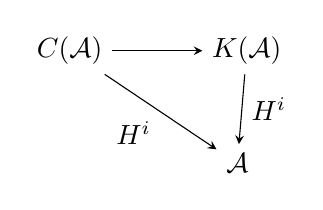
\begin{tikzpicture}[>=stealth]
  \node (c) at (0,1.43) {$C(\mathcal A)$};
  \node (k) at (2.25,1.43) {$K(\mathcal A)$};
  \node (a) at (2.13,0) {$\mathcal A$};
  \draw[->] (c) -- (k);
  \draw[->] (c) -- node[below left] {$H^i$} (a);
  \draw[->] (k) -- node[right] {$H^i$} (a);
\end{tikzpicture}}\endgroup}
\end{GelfandAdjacentEvidence}
\begin{GelfandAdjacentEvidence}{GELFAND-P001393}{3}


На морфизмах \(H^i\) тоже очев. образом определяется.

\uline{Определение.}
\[
\varphi\colon X^\bullet
\underset{\text{в кат. }K(\mathcal A)}{\longrightarrow}Y^\bullet
\]
наз. \uwave{квазиизоморфизмом} если он индуц. изоморфизм
\[
H^i(X^\bullet)\longrightarrow H^i(Y^\bullet).
\]

\uwave{Производная категория}

\uwave{Упражнение 4.}\quad Пусть есть 3 комплекса
\SourceFigure{GELFAND-P001393}{fraction-span}{%
\begingroup\color{black}\GelfandFitDiagram{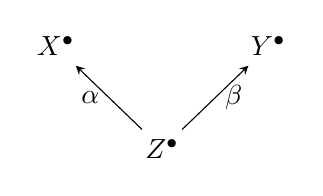
\begin{tikzpicture}[>=stealth]
  \node (x) at (0,1.3) {$X^\bullet$};
  \node (y) at (2.7,1.3) {$Y^\bullet$};
  \node (z) at (1.35,0) {$Z^\bullet$};
  \draw[->] (z) -- node[left] {$\alpha$} (x);
  \draw[->] (z) -- node[right] {$\beta$} (y);
\end{tikzpicture}}\endgroup}
\end{GelfandAdjacentEvidence}
\begin{GelfandAdjacentEvidence}{GELFAND-P001393}{4}

и морфизмы, причём \(\alpha\) --- квазиизоморфизм.

Тогда сущ. диаграмма (коммутативная)
\SourceFigure{GELFAND-P001393}{fraction-square}{%
\begingroup\color{black}\GelfandFitDiagram{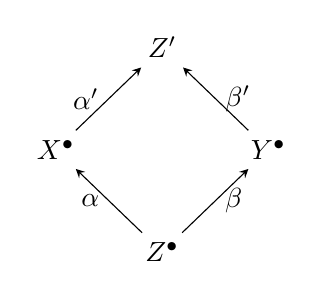
\begin{tikzpicture}[>=stealth]
  \node (x) at (0,1.3) {$X^\bullet$};
  \node (y) at (2.7,1.3) {$Y^\bullet$};
  \node (z) at (1.35,0) {$Z^\bullet$};
  \node (zp) at (1.35,2.6) {$Z'$};
  \draw[->] (z) -- node[left] {$\alpha$} (x);
  \draw[->] (z) -- node[right] {$\beta$} (y);
  \draw[->] (x) -- node[left] {$\alpha'$} (zp);
  \draw[->] (y) -- node[right] {$\beta'$} (zp);
\end{tikzpicture}}\endgroup}
\end{GelfandAdjacentEvidence}
\begin{GelfandAdjacentEvidence}{GELFAND-P001393}{5}

[слева от диаграммы зачёркнуто:
«в к-рой»?\textsuperscript{?}.]
\Unclear{GELFAND-P001393}{cancelled-left}{«в к-рой»?}
\end{GelfandAdjacentEvidence}
\begin{GelfandAdjacentEvidence}{GELFAND-P001393}{6}


в к-рой \(\beta'\) --- квазиизоморфизм.

То же справедливо, если начинать с диагр.
\SourceFigure{GELFAND-P001393}{fraction-cospan}{%
\begingroup\color{black}\GelfandFitDiagram{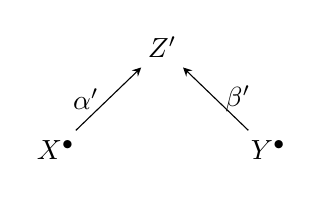
\begin{tikzpicture}[>=stealth]
  \node (x) at (0,0) {$X^\bullet$};
  \node (y) at (2.7,0) {$Y^\bullet$};
  \node (zp) at (1.35,1.3) {$Z'$};
  \draw[->] (x) -- node[left] {$\alpha'$} (zp);
  \draw[->] (y) -- node[right] {$\beta'$} (zp);
\end{tikzpicture}}\endgroup}
\end{GelfandAdjacentEvidence}

с квазиизоморфизмом \(\alpha'\).


\Needspace{7\baselineskip}
\begin{GelfandAdjacentEvidence}{GELFAND-P001394}{1}
\SourcePage{GELFAND-P001394}{unlabelled}

\uwave{Производная категория} \(D(\mathcal A)\)

Объекты \(=\) объекты \(K(\mathcal A)\) (т.е. комплексы)

Морфизмы [вставлено над строкой: \(X^\bullet\longrightarrow Y^\bullet\)] ---
классы эквив. диаграмм
\SourceFigure{GELFAND-P001394}{derived-roof}{%
\begingroup\color{black}\GelfandFitDiagram{\begin{tikzpicture}[>=stealth]
  \node (x) at (0,1.3) {$X^\bullet$};
  \node (y) at (2.7,1.3) {$Y^\bullet$};
  \node (z) at (1.35,0) {$Z^\bullet$};
  \node at (4.12,.66) {$\beta\alpha^{-1}$};
  \draw[->] (z) -- node[left] {$\alpha$} (x);
  \draw[->] (z) -- node[right] {$\beta$} (y);
\end{tikzpicture}}\endgroup}
\end{GelfandAdjacentEvidence}
\begin{GelfandAdjacentEvidence}{GELFAND-P001394}{2}


(\(\alpha\) --- квазиизоморфизм)

по отнош. эквивалентности, \uwave{порожденному} элем. отношением
\EvidenceBlock{GELFAND-P001394}{elementary-abbrev}{Сокращение читается «элем.».}{Запись в рукописи.}
\end{GelfandAdjacentEvidence}
\begin{GelfandAdjacentEvidence}{GELFAND-P001394}{3}


[зачёркнуто: «Есть»? / «Если»?\textsuperscript{?}.]
\Unclear{GELFAND-P001394}{cancelled-there}{«Есть»? / «Если»?}
\end{GelfandAdjacentEvidence}
\begin{GelfandAdjacentEvidence}{GELFAND-P001394}{4}


(Есть функтор \(K(\mathcal A)\longrightarrow D(\mathcal A)\))

\SourceFigure{GELFAND-P001394}{roof-refinement}{%
\begingroup\color{black}\GelfandFitDiagram{\begin{tikzpicture}[>=stealth]
  \node (x) at (0,2.6) {$X^\bullet$};
  \node (y) at (2.7,2.6) {$Y^\bullet$};
  \node (z) at (1.35,1.28) {$Z^\bullet$};
  \node (t) at (1.35,0) {$T$};
  \draw[->] (z) -- node[left] {$\alpha$} (x);
  \draw[->] (z) -- node[right] {$\beta$} (y);
  \draw[->] (t) -- node[right] {$\gamma$} (z);
\end{tikzpicture}}\endgroup}
\end{GelfandAdjacentEvidence}
\begin{GelfandAdjacentEvidence}{GELFAND-P001394}{5}


\(\beta\alpha^{-1}\sim\beta\gamma(\alpha\gamma)^{-1}\),
где \(\gamma\) --- квазиизоморфизм.
\Unclear{GELFAND-P001394}{fraction-relation}{Знак отношения похож на \(\sim\). Наводка затрудняет чтение отдельных штрихов этого знака и следующей \(\beta\).}
\end{GelfandAdjacentEvidence}
\begin{GelfandAdjacentEvidence}{GELFAND-P001394}{6}


\SourceFigure{GELFAND-P001394}{equivalent-roofs}{%
\resizebox{\linewidth}{!}{%
\begingroup\color{black}\GelfandFitDiagram{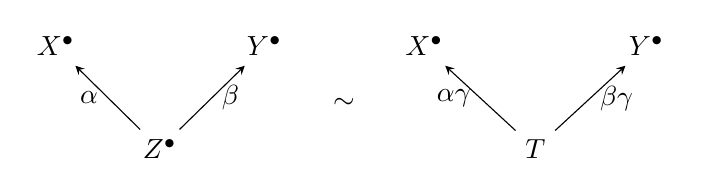
\begin{tikzpicture}[>=stealth]
  \node (x) at (0,1.30) {$X^\bullet$};
  \node (y) at (2.65,1.30) {$Y^\bullet$};
  \node (z) at (1.32,0) {$Z^\bullet$};
  \node at (3.66,.58) {$\sim$};
  \node (rx) at (4.68,1.30) {$X^\bullet$};
  \node (ry) at (7.50,1.30) {$Y^\bullet$};
  \node (t) at (6.09,0) {$T$};
  \draw[->] (z) -- node[left] {$\alpha$} (x);
  \draw[->] (z) -- node[right] {$\beta$} (y);
  \draw[->] (t) -- node[left] {$\alpha\gamma$} (rx);
  \draw[->] (t) -- node[right] {$\beta\gamma$} (ry);
\end{tikzpicture}}\endgroup}}
\end{GelfandAdjacentEvidence}
\begin{GelfandAdjacentEvidence}{GELFAND-P001394}{7}


Теперь уже морфизмы можно компоновать.

\SourceFigure{GELFAND-P001394}{roof-composition}{%
\resizebox{\linewidth}{!}{%
\begingroup\color{black}\GelfandFitDiagram{\begin{tikzpicture}[>=stealth]
  \node (x) at (0,2.45) {$X^\bullet$};
  \node (y) at (2.6,2.45) {$Y^\bullet$};
  \node (w) at (5.2,2.45) {$W$};
  \node (z) at (1.30,1.2) {$Z^\bullet$};
  \node (t) at (3.90,1.2) {$T$};
  \node (s) at (2.6,-.12) {$S$};
  \draw[->] (z) -- (x);
  \draw[->] (z) -- (y);
  \draw[->] (t) -- (y);
  \draw[->] (t) -- (w);
  \draw[->] (s) -- (z);
  \draw[->] (s) -- (t);
  \draw[->] (4.84,.34) -- (4.13,.34);
  \node[right,align=left] at (4.93,.34) {достраиваем \uwave{по лемме}};
\end{tikzpicture}}\endgroup}}
\end{GelfandAdjacentEvidence}


композиция --- внешняя сторона диаграммы.


\Needspace{7\baselineskip}
\begin{GelfandAdjacentEvidence}{GELFAND-P001395}{1}
\SourcePage{GELFAND-P001395}{unlabelled}

\uline{19.10.87.}\quad \uline{Сем. Гельфанда.}

\uwave{И. М. Гельфанд}\quad \uuline{Вычисление сумм \(k\)-х степеней и прочих сумм}

\Unclear{GELFAND-P001395}{speaker-parenthesis}{(по недавней мысли?)}
\end{GelfandAdjacentEvidence}
\begin{GelfandAdjacentEvidence}{GELFAND-P001395}{2}


\[
F'(x)=f(x)\qquad f(x)=x^k,\qquad F(x)=\frac{x^{k+1}}{k+1}
\]
\begin{align*}
F(2)-F(1)&=\frac{f(1)}{1!}+\frac{f'(1)}{2!}+\frac{f''(1)}{3!}+\ldots\\
F(3)-F(2)&=\frac{f(2)}{1!}+\frac{f'(2)}{2!}+\frac{f''(2)}{3!}+\ldots\\[8pt]
F(n+1)-F(n)&=f(n)+\frac{f'(n)}{2!}+\frac{f''(n)}{3!}+\ldots
\end{align*}
\rule{9cm}{.3pt}
\[
F(n+1)-F(1)=S_0+\frac{S_1}{2!}+\frac{S_2}{3!}+\ldots
\]
аналогично,
\begin{align*}
f(n+1)-f(1)&=S_1+\frac{S_2}{2!}+\ldots\\
f'(n+1)-f'(1)&=S_2+\frac{S_3}{2!}+\ldots\\
\ldots\qquad&\ldots\\
f^{(p)}(n+1)-f^{(p)}(1)&=\ldots\quad S_p+\ldots
\end{align*}
\EvidenceBlock{GELFAND-P001395}{system-last-index}{В последней строке \(S_p\).}{Запись в рукописи.}
\end{GelfandAdjacentEvidence}
\begin{GelfandAdjacentEvidence}{GELFAND-P001395}{3}


[Справа от системы] Здесь
\begin{align*}
S_0&=f(1)+f(2)+\ldots+f(n)\\
S_1&=f'(1)+f'(2)+\ldots+f'(n)\\
&\ldots\\
S_k&=f^{(k)}(1)+f^{(k)}(2)+\ldots+f^{(k)}(n)
\end{align*}

Отсюда
[слева от определителя зачёркнуто:
«det»?\textsuperscript{?}]
\Unclear{GELFAND-P001395}{determinant-cancellation}{«det»?}
\end{GelfandAdjacentEvidence}
\begin{GelfandAdjacentEvidence}{GELFAND-P001395}{4}

\SourceFigure{GELFAND-P001395}{determinant-layout}{%
\(\displaystyle S_0=\frac{
\begin{vmatrix}
F(n+1)-F(1)&\frac{1}{2!}&\frac{1}{3!}&\ldots\\
f(n+1)-f(1)&1&\frac{1}{2!}&\\
f'(n+1)-f'(1)&0&1&\\
\ldots&0&0&
\end{vmatrix}}{1}\)}
\end{GelfandAdjacentEvidence}
\begin{GelfandAdjacentEvidence}{GELFAND-P001395}{5}


Разложим по 1-му столбцу
\[
S_0=A_0\bigl(F(n+1)-F(1)\bigr)
+A_1\bigl(f(n+1)-f(1)\bigr)+\ldots
\]
коэфф. универ. --- годится для \(\forall\) ф-и!!

Подставим \(f(x)=e^{tx}\)

возникают ленточные детерминанты!

[зачёркнуто:
возможно \(S_0=A_0\)\textsuperscript{?}]
\Unclear{GELFAND-P001395}{exponential-cancellation}{возможно \(S_0=A_0\)}
\end{GelfandAdjacentEvidence}
\begin{GelfandAdjacentEvidence}{GELFAND-P001395}{6}

\[
\frac{\dfrac{1}{n+1}e^{t(n+1)}-e}{e^t-1}
\]
\EvidenceBlock{GELFAND-P001395}{exponential-fraction}{Числитель
\(\frac{1}{n+1}e^{t(n+1)}-e\).}{Запись в рукописи.}
\end{GelfandAdjacentEvidence}
\begin{GelfandAdjacentEvidence}{GELFAND-P001395}{7}

разложим [зачёркнуто:
«ряд»?\textsuperscript{?}]
\Unclear{GELFAND-P001395}{series-cancellation}{«ряд»?}
\end{GelfandAdjacentEvidence}
\begin{GelfandAdjacentEvidence}{GELFAND-P001395}{8}

по \(t\)\quad \(\Longrightarrow\) \uline{числа Бернулли}

\uline{Задача.} Симм. группа \(S_n\) определяется
\EvidenceBlock{GELFAND-P001395}{symmetric-group-predicate}{«определяется».}{Запись в рукописи.}
\end{GelfandAdjacentEvidence}
\begin{GelfandAdjacentEvidence}{GELFAND-P001395}{9}

[вставлено над строкой: (обр[…]\textsuperscript{?} \(s_1,\ldots,s_{n-1}\))]
\Unclear{GELFAND-P001395}{group-generator-abbreviation}{Видно начало «обр». Конец сокращения неясен.}
\end{GelfandAdjacentEvidence}

соотношениями
\[
s_i^2=1,\qquad s_i s_j=s_j s_i\quad\text{при }\lvert i-j\rvert\ge2,
\qquad (s_i s_{i+1})^3=1
\]
Рассм. параболич. подгруппу
\[
G=\Sigma_n,\qquad H=\Sigma_k\times\Sigma_{n-k},\qquad G\supset H
\]
\[
\mathcal A=\mathbb C[G]=
\left\{\sum_{g\in G}a_g g,\quad a_g\in\mathbb C\right\}
\]


\Needspace{7\baselineskip}
\begin{GelfandAdjacentEvidence}{GELFAND-P001396}{1}
\SourcePage{GELFAND-P001396}{23}

\[
\mathcal A\supset\underset{\substack{\vert\\\text{подалгебра}}}{\mathcal A'}
=\{x\in A,\ xh=hx=x\text{ для любых }h\in H\}
\]

[зачёркнуто: неразборчивый знак]
\Unclear{GELFAND-P001396}{heading-cancellation}{неразборчивый знак}
\end{GelfandAdjacentEvidence}
\begin{GelfandAdjacentEvidence}{GELFAND-P001396}{2}

\uuline{Бейлинсон А.}\quad (продолжение)

\uline{Производные категории.}

\SourceFigure{GELFAND-P001396}{category-chain}{%
\resizebox{\linewidth}{!}{%
\begingroup\color{black}\GelfandFitDiagram{\begin{tikzpicture}[>=stealth]
  \node (a) at (0,2.7) {$\mathcal A$};
  \node (c) at (0,1.8) {$C(\mathcal A)$};
  \node (k) at (0,.9) {$K(\mathcal A)$};
  \node (d) at (0,0) {$D(\mathcal A)$};
  \node[right] at (.72,2.7) {--- абелева категория};
  \node[right] at (.72,1.8) {--- кат. комплексов над \(\mathcal A\)};
  \node[right] at (.72,.9) {--- гомотопич. категория};
  \node[right] at (.72,0) {--- производная категория};
  \draw[->] (a) -- (c);
  \draw[->] (c) -- (k);
  \draw[->] (k) -- (d);
\end{tikzpicture}}\endgroup}}
\end{GelfandAdjacentEvidence}
\begin{GelfandAdjacentEvidence}{GELFAND-P001396}{3}


объекты \(D(\mathcal A)\) --- комплексы, а морфизмы --- классы эквив. диаграмм

\SourceFigure{GELFAND-P001396}{roof-cancellation}{%
\begingroup\color{black}\GelfandFitDiagram{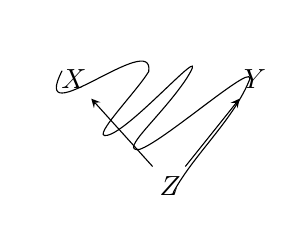
\begin{tikzpicture}[>=stealth]
  \node (x) at (0,1.35) {$X$};
  \node (y) at (2.30,1.35) {$Y$};
  \node (z) at (1.22,0) {$Z$};
  \draw[->] (z) -- (x);
  \draw[->] (z) -- (y);
  \draw (-.15,1.46) .. controls (-.58,.61) and (1.03,2.00) .. (.95,1.45)
    .. controls (.79,1.18) and (.11,.50) .. (.48,.66)
    .. controls (.84,.83) and (1.78,1.92) .. (1.43,1.36)
    .. controls (1.11,.88) and (.56,.43) .. (.83,.46)
    .. controls (1.15,.56) and (2.38,1.66) .. (2.22,1.32)
    .. controls (2.01,.82) and (1.51,.38) .. (1.26,-.09);
\end{tikzpicture}}\endgroup
\par{\small Диаграмма зачёркнута. Правая стрелка частично скрыта.}}
\end{GelfandAdjacentEvidence}
\begin{GelfandAdjacentEvidence}{GELFAND-P001396}{4}


\SourceFigure{GELFAND-P001396}{shorter-roof-square}{%
\begingroup\color{black}\GelfandFitDiagram{\begin{tikzpicture}[>=stealth]
  \node (x) at (0,1.04) {$X$};
  \node (y) at (2.66,1.53) {$Y$};
  \node (z) at (.68,0) {$Z$};
  \node (zp) at (1.88,2.57) {$Z'$};
  \draw[->] (x) -- (zp);
  \draw[->] (z) -- (y);
  \draw[->,shorten <=4pt,shorten >=3pt] (y) -- (zp);
  \draw[->,shorten <=4pt,shorten >=3pt] (z) -- (x);
\end{tikzpicture}}\endgroup\par (квазиизоморфизмы короче).}
\end{GelfandAdjacentEvidence}
\begin{GelfandAdjacentEvidence}{GELFAND-P001396}{5}


\uline{Пример 1.}\quad Пусть \(X\) --- комплекс с
[зачёркнуто: «со»?]
\(H^i(X)=0\) при \(i\ne0\).
Тогда \(X\) канонически квазиизоморфен \(H^0(X)\):


\Unclear{GELFAND-P001396}{example-cancellation}{«со»?}
\end{GelfandAdjacentEvidence}
\begin{GelfandAdjacentEvidence}{GELFAND-P001396}{6}

\[
X\cong H^0(X)\text{ в }D(\mathcal A)
\]
(В гомотопической категории это не так!)

Для комплекса \(X\) введем подкомплекс \(\tau_{\leq0}(X)\in X\):
\begin{equation*}
\tau_{\leq0}(X)^i=
\begin{cases}
X^i,&i<0\\
\ker(d\colon X^0\to X^1),&i=0\\
0,&i>0
\end{cases}
\tag{1}
\end{equation*}

Легко видеть, что
\begin{equation*}
H^j(\tau_{\leq0}(X))=
\begin{cases}
H^j(X),&j\leq0\\
0,&j>0
\end{cases}
\tag{2}
\end{equation*}
Диаграмма
\SourceFigure{GELFAND-P001396}{truncation-diagram}{%
\resizebox{\linewidth}{!}{%
\begingroup\color{black}\GelfandFitDiagram{\begin{tikzpicture}[>=stealth]
  \node (x) at (0,1.75) {$X$};
  \node (h) at (3.35,1.45) {$H^0(X)$};
  \node (t) at (1.4,0) {$\tau_{\leq0}(X)$};
  \node at (-.95,.93) {(3)};
  \draw[->] (t) -- node[above right] {$2$?} (x);
  \draw[->] (t) -- node[below right] {$\sim$} (h);
  \node[align=left] at (-.07,.11) {\scriptsize кан. вкл.};
  \draw[thin] (4.23,.45) .. controls (4.37,.70) and (4.56,.44) .. (4.38,.33);
\end{tikzpicture}}\endgroup}\par{\small Знак у левой стрелки похож на 2 или повёрнутую тильду.}}
\end{GelfandAdjacentEvidence}
\begin{GelfandAdjacentEvidence}{GELFAND-P001396}{7}

задаёт искомый изоморфизм в \(D(\mathcal A)\).

[зачёркнуто:
Этот же комплекс может быть спроецирован на…?\textsuperscript{?}]
\Unclear{GELFAND-P001396}{cancelled-bottom-sentence}{Этот же комплекс может быть спроецирован на…?}
\end{GelfandAdjacentEvidence}
\begin{GelfandAdjacentEvidence}{GELFAND-P001396}{8}


\uline{Замечание.} комплекс \(X\) с несколькими отл. от \(0\) группами \(H^i\) 
\uline{не} квазиизоморфен (вообще говоря) сумме, а если
[вставлено над строкой: (квази)] есть, то неоднозначн.\textsuperscript{?} способом.
\Unclear{GELFAND-P001396}{ending-reading}{Видно «неоднозначн… способом». Окончание первого слова неясно.}
\end{GelfandAdjacentEvidence}



\Needspace{7\baselineskip}
\begin{GelfandAdjacentEvidence}{GELFAND-P001397}{1}
\SourcePage{GELFAND-P001397}{unlabelled}

\uline{Структура триангулированной категории}

\(K(A)\) и \(D(A)\) не явл. абелевыми категориями.

\uline{Упражнение 1.}\quad Проверить, что
\[
K(A)\text{ --- абелева}\quad\Longleftrightarrow\quad
\mathcal A\text{ полупроста}
\]
(\(\mathcal A\) --- полупроста \(\Longleftrightarrow\
[(\forall\text{ объект})=(\text{прямая сумма неприводимых})]\)).

\uline{Конус морфизма.}

Пусть \(f\colon X\longrightarrow Y\) морфизм комплексов

\SourceFigure{GELFAND-P001397}{bicomplex-diagram}{%
\begingroup\color{black}\GelfandFitDiagram{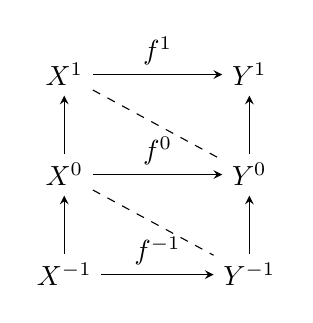
\begin{tikzpicture}[>=stealth]
  \node (x1) at (0,2.54) {$X^1$}; \node (y1) at (2.35,2.54) {$Y^1$};
  \node (x0) at (0,1.27) {$X^0$}; \node (y0) at (2.35,1.27) {$Y^0$};
  \node (xm) at (0,0) {$X^{-1}$}; \node (ym) at (2.35,0) {$Y^{-1}$};
  \draw[->] (x1) -- node[above] {$f^1$} (y1);
  \draw[->] (x0) -- node[above] {$f^0$} (y0);
  \draw[->] (xm) -- node[above] {$f^{-1}$} (ym);
  \draw[->] (xm) -- (x0); \draw[->] (x0) -- (x1);
  \draw[->] (ym) -- (y0); \draw[->] (y0) -- (y1);
  \draw[dashed] (x1) -- (y0); \draw[dashed] (x0) -- (ym);
\end{tikzpicture}}\endgroup}
\end{GelfandAdjacentEvidence}
\begin{GelfandAdjacentEvidence}{GELFAND-P001397}{2}

[Справа] рассм. это всё как бикомплекс, т.е. напишем комплекс
\[
C(f)^i=Y^i\oplus X^{i+1}
\]
\EvidenceBlock{GELFAND-P001397}{cone-coordinate-order}{В формуле конуса \(Y^i\oplus X^{i+1}\).}{Запись в рукописи.}
\end{GelfandAdjacentEvidence}
\begin{GelfandAdjacentEvidence}{GELFAND-P001397}{3}

\[
d(x,y)=(-d(x),d(y)+f(x))
\]

Имеется последовательность
\begin{equation*}
C(f[-1])\longrightarrow X\overset{f}{\longrightarrow}Y
\underset{\substack{g\\\text{вкл.}}}{\longrightarrow}C(f)
\longrightarrow X[1]\longrightarrow
\tag{4}
\end{equation*}
[Над стрелкой зачёркнуто \(Y\to C(f)\):
неразборчивая запись.]
\Unclear{GELFAND-P001397}{sequence-arrow-cancellation}{неразборчивая запись}
\end{GelfandAdjacentEvidence}
\begin{GelfandAdjacentEvidence}{GELFAND-P001397}{4}

[Зачёркнуто перед \(C(f)\):
\(X\)? / \(Y\)?\textsuperscript{?}.]
\Unclear{GELFAND-P001397}{sequence-object-cancellation}{\(X\)? / \(Y\)?}
\end{GelfandAdjacentEvidence}
\begin{GelfandAdjacentEvidence}{GELFAND-P001397}{5}

[Под \(X[1]\): сдвиг градуировки и изменён знак \(d\).]
\[
\longrightarrow Y(1)\longrightarrow C(f[1])\longrightarrow X[2]\longrightarrow
\]
\Unclear{GELFAND-P001397}{sequence-shifted-cone}{Конечная скобка стоит после сдвига: \(C(f[1])\). Между \(f\) и \([1]\) видна неразборчивая зачёркнутая запись.}
\end{GelfandAdjacentEvidence}
\begin{GelfandAdjacentEvidence}{GELFAND-P001397}{6}

[Между \(X\) и \([2]\) зачёркнуто:
знак, похожий на скобку\textsuperscript{?}]
\Unclear{GELFAND-P001397}{sequence-shift-cancellation}{знак, похожий на скобку}
\end{GelfandAdjacentEvidence}
\begin{GelfandAdjacentEvidence}{GELFAND-P001397}{7}


она перех. в себя при сдвиге на 3 шага.
В гомотопич. категории она перех. в себя при сдвиге на шаг.

\begin{equation*}
Y\overset{g}{\longrightarrow}C(f)\longrightarrow C(g)
\tag{5}
\end{equation*}

(6) \uline{Утвержд.}\quad В \(K(A)\) комплекс \(C(g)=X[1]\).

Имеется отображение:
\SourceFigure{GELFAND-P001397}{cone-projection-diagram}{%
\begingroup\color{black}\GelfandFitDiagram{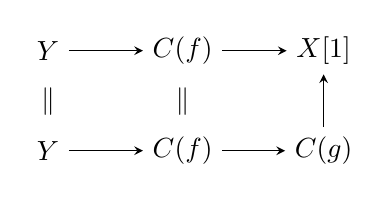
\begin{tikzpicture}[>=stealth]
  \node (y) at (0,1.27) {$Y$}; \node (ry) at (0,0) {$Y$};
  \node (f) at (1.71,1.27) {$C(f)$}; \node (rf) at (1.71,0) {$C(f)$};
  \node (x) at (3.50,1.27) {$X[1]$}; \node (g) at (3.50,0) {$C(g)$};
  \draw[->] (y) -- (f); \draw[->] (f) -- (x);
  \draw[->] (ry) -- (rf); \draw[->] (rf) -- (g);
  \node at (0,.63) {$\parallel$}; \node at (1.71,.63) {$\parallel$};
  \draw[->] (g) -- (x);
\end{tikzpicture}}\endgroup}
\end{GelfandAdjacentEvidence}


А именно,
\[
C(g)^i=C(f)^i\oplus Y^{i+1}=X^{i+1}\oplus Y^i\oplus Y^{i+1}
\]
проектируется на \(X^{i+1}\).


\Needspace{7\baselineskip}
\begin{GelfandAdjacentEvidence}{GELFAND-P001398}{1}
\SourcePage{GELFAND-P001398}{24}

\uline{Упражнение 2.} Проверить, что это морфизм комплексов и изоморфизм в гомотопической категории.

\uline{Упражнение 3.} Найти в \(K(A)\) конусы
\(C(\underset{\substack{\vert\\\text{тожд. отобр.}}}{id})\)
и
\(C(\underset{\substack{\vert\\\text{нулевое отобр.}}}{0})\).

\uline{Определение 1.} Треугольником в \(K(A)\) или \(D(A)\) называется диаграмма

\SourceFigure{GELFAND-P001398}{triangle-sequence}{%
\begingroup\color{black}\GelfandFitDiagram{\(\begin{aligned}
\cdots\longrightarrow Z[-1]\xrightarrow{\gamma[-1]} X
  \xrightarrow{\alpha}Y\xrightarrow{\beta}Z\\
{}\xrightarrow{\gamma}X[1]\xrightarrow{\alpha[1]}Y[1]
  \xrightarrow{\beta[1]}Z[1]\xrightarrow{\gamma[1]}\cdots
\end{aligned}\)}\endgroup}
\end{GelfandAdjacentEvidence}
\begin{GelfandAdjacentEvidence}{GELFAND-P001398}{2}


\SourceFigure{GELFAND-P001398}{cancelled-sketch}{%
\begingroup\color{black}\GelfandFitDiagram{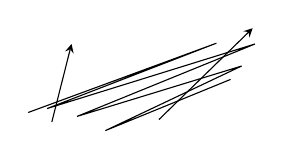
\begin{tikzpicture}[>=stealth,x=1cm,y=1cm]
  \draw[->] (.33,.03) -- (.58,1.02);
  \draw[->] (1.69,.06) -- (2.88,1.22);
  \draw[thin] (.03,.15) -- (2.42,1.03) -- (.27,.20) -- (2.91,1.02)
    -- (.65,.10) -- (2.74,.74) -- (1.01,-.08) -- (2.60,.57);
\end{tikzpicture}}\endgroup
\par{\small Зачёркнутый набросок. Видны две стрелки; возможные подписи неразборчивы.}}
\end{GelfandAdjacentEvidence}
\begin{GelfandAdjacentEvidence}{GELFAND-P001398}{3}


\uuline{Опред. 2.} Точным треугольником в \(K(A)\) или \(D(A)\) наз. треугольник, изоморфный треугольнику:

\SourceFigure{GELFAND-P001398}{exact-triangle}{%
\begingroup\color{black}\GelfandFitDiagram{\(\longrightarrow X\xrightarrow{f}Y\xrightarrow{g}C(f)
  \longrightarrow X[1]\longrightarrow Y[1]\longrightarrow\cdots\)}\endgroup}
\end{GelfandAdjacentEvidence}



\Needspace{7\baselineskip}
\begin{GelfandAdjacentEvidence}{GELFAND-P001399}{1}
\SourcePage{GELFAND-P001399}{unlabelled}

\uline{9/XI-87 г.}\qquad \uuline{Сем. Гельфанда}

[Зачёркнуто: Ласку.]\qquad \uline{Ласку}

\uline{И. М. Г. по мотивам Ласку}
(красивые / правильные\textsuperscript{?} ряды)

\Unclear{GELFAND-P001399}{heading-parenthesis}{красивые / правильные}
\end{GelfandAdjacentEvidence}
\begin{GelfandAdjacentEvidence}{GELFAND-P001399}{2}



Полиномы Шуберта.

Рассм. многочлен
\begin{equation*}
P=\alpha u+\beta u+\gamma w+\cdots \tag{1}
\end{equation*}
\EvidenceBlock{GELFAND-P001399}{equation-1-second-variable}{Второй одночлен в (1): \(\beta u\).}{Запись в рукописи.}
\end{GelfandAdjacentEvidence}
\begin{GelfandAdjacentEvidence}{GELFAND-P001399}{3}


\(u,v,w\) [Зачёркнуто: возможно, \(\alpha,\beta,\gamma\)\textsuperscript{?}] — одночлены.

\Unclear{GELFAND-P001399}{cancelled-coefficients}{возможно, \(\alpha,\beta,\gamma\)}
\end{GelfandAdjacentEvidence}
\begin{GelfandAdjacentEvidence}{GELFAND-P001399}{4}



В нашем случае будет \(u,v,w,\)
[Зачёркнуто: знак неразборчив]
\(\ldots=x_1,x_2,\ldots,x_n\).

\Unclear{GELFAND-P001399}{cancelled-after-w}{знак неразборчив}
\end{GelfandAdjacentEvidence}
\begin{GelfandAdjacentEvidence}{GELFAND-P001399}{5}



\(\alpha,\beta,\gamma,\ldots\) — числа.

Многочлены [Зачёркнуто: ф-я / ф-и\textsuperscript{?}]
\(S^m(P)\) [Зачёркнуто: возможно, Шура\textsuperscript{?}]
определяются по ф-ле


\Unclear{GELFAND-P001399}{cancelled-before-sm}{«ф-я» / «ф-и»?}
\end{GelfandAdjacentEvidence}
\begin{GelfandAdjacentEvidence}{GELFAND-P001399}{6}

\Unclear{GELFAND-P001399}{cancelled-after-sm}{возможно, Шура}
\end{GelfandAdjacentEvidence}
\begin{GelfandAdjacentEvidence}{GELFAND-P001399}{7}

\begin{equation*}
\sum_{m\ge 0}^{\infty}z^m S^m(P)
=\frac{1}{(1-zu)^\alpha(1-zv)^\beta\ldots} \tag{2}
\end{equation*}
\EvidenceBlock{GELFAND-P001399}{equation-2-lower-bound}{Нижний предел в (2): \(m\ge 0\).}{Запись в рукописи.}
\end{GelfandAdjacentEvidence}
\begin{GelfandAdjacentEvidence}{GELFAND-P001399}{8}


\[
\alpha=\beta=\gamma=\cdots=1\quad\Rightarrow
\]
\begin{equation*}
S^m(x_1+x_2+\cdots+x_n)
=\sum_{i_1\le i_2\le\cdots\le i_m}x_{i_1}x_{i_2}\cdots x_{i_m} \tag{3}
\end{equation*}

Например,
\[
S^2(x_1+x_2)=x_1^2+x_1x_2+x_2^2.
\]

Рассмотрим ганкелеву матрицу (бес. порядка)
\begin{equation*}
\begin{pmatrix}
S^0(P)&S^1(P)&S^2(P)&\ldots\\
S^{-1}(P)&S^0(P)&S^{4?}(P)&\ldots\\
&&&
\end{pmatrix},\qquad S^{-i}(P)=0\text{ при }i>0. \tag{4}
\end{equation*}
\Unclear{GELFAND-P001399}{matrix-row-2-col-3}{Показатель в позиции \((2,3)\) в (4) похож на \(4\). Возможна \(1\).}
\end{GelfandAdjacentEvidence}


(см. кн. \uline{Ахиезера} о пробл. моментов)

Умножению рядов (2) соответствует умножение матриц (4).


\Needspace{7\baselineskip}
\begin{GelfandAdjacentEvidence}{GELFAND-P001400}{1}
\SourcePage{GELFAND-P001400}{30}

\uline{Тема по теории операторов, к-рую И. М. Г. предложил}
Бирману / Бурману\textsuperscript{?}:

\Unclear{GELFAND-P001400}{heading-recipient}{Бирману / Бурману}
\end{GelfandAdjacentEvidence}
\begin{GelfandAdjacentEvidence}{GELFAND-P001400}{2}



Связать\textsuperscript{?}
\(K\)-функтор в теории операторов

\Unclear{GELFAND-P001400}{heading-verb}{Вероятно, «Связать».}
\end{GelfandAdjacentEvidence}
\begin{GelfandAdjacentEvidence}{GELFAND-P001400}{3}



(на 15 лет позже уже это сделал Сато)

и это стало модой.

\uline{Единств. теорема из теории матриц}

Рассм. матрицу \(A\): \(f_{\alpha\beta}=f(\alpha,\beta)\)
и все её миноры \(k\)-го порядка: это тоже матрица (присоед. матр. \(k\)-го порядка) \(\Lambda^k(A)\). Тогда
\begin{equation*}
\Lambda^k(AB)=\Lambda^k(A)\Lambda^k(B) \tag{5}
\end{equation*}

Номера строк выгодно обозначать \(i_1+1,i_2+2,\ldots,i_p+p\), а столбцов
\(j_1+1,j_2+2,\ldots,j_p+p\)
\[
\left|\begin{aligned}
i_1&\le i_2\le\cdots\le i_p\\
j_1&\le\cdots\le j_p
\end{aligned}\right.
\]

\begin{equation*}
\begin{gathered}
S_{J\mid I}(P)\\
\text{— соотв. минор, наз. }\text{\uline{косая функция Шура}}.
\end{gathered} \tag{6}
\end{equation*}
\[
S_{J\mid 0}(P)\quad\text{— обычная ф-я Шура.}
\]

[Зачёркнуто: Тогда] Можно рассм. многочлен (Якоби)
\begin{equation*}
\frac{\begin{vmatrix}
x_1^{j_1}&x_1^{j_2+1}&\ldots&x_1^{j_p+p-1}\\
x_2^{j_1}&x_2^{j_2+1}&\ldots&x_2^{j_p+p-1}\\
\ldots&\ldots&\ldots&\ldots
\end{vmatrix}}{\begin{vmatrix}
1&x_1&\ldots&x_1^{p-1}\\
1&x_2&\ldots&x_2^{p-1}\\
&&&\\
1&x_p&\ldots&x_p^{p-1}
\end{vmatrix}} \tag{7}
\end{equation*}
\Unclear{GELFAND-P001400}{numerator-first-column-cancellations}{В первых двух строках числителя после \(j_1\) зачёркнуто, вероятно, \(+1\).}
\end{GelfandAdjacentEvidence}
\begin{GelfandAdjacentEvidence}{GELFAND-P001400}{4}

\Unclear{GELFAND-P001400}{right-of-numerator}{Справа от числителя: \(1\) или одиночный косой штрих.}
\end{GelfandAdjacentEvidence}
\begin{GelfandAdjacentEvidence}{GELFAND-P001400}{5}


(\(8\)\textsuperscript{?})
([Вписано над строкой: \uline{Упр}] проверить, что числитель делится на знаменатель!)

\Unclear{GELFAND-P001400}{exercise-number}{Вероятно, \(8\). Возможна \(7\).}
\end{GelfandAdjacentEvidence}
\begin{GelfandAdjacentEvidence}{GELFAND-P001400}{6}



[Зачёркнуто: ко / но\textsuperscript{?}.]
Это симметрич. ф-я, но коэффициенты явно не
[Зачёркнуто: неразборчиво]
[Вписано над строкой: \uline{пишутся}] и до сих пор исследуются.

\Unclear{GELFAND-P001400}{cancelled-before-eto}{«ко» / «но»?}
\end{GelfandAdjacentEvidence}
\begin{GelfandAdjacentEvidence}{GELFAND-P001400}{7}

\Incomplete{GELFAND-P001400}{cancelled-right-word}{слово под вставленным «пишутся» неразборчиво}
\end{GelfandAdjacentEvidence}
\begin{GelfandAdjacentEvidence}{GELFAND-P001400}{8}



[На левом поле: (первые шаги,\textsuperscript{?}
при решении\textsuperscript{?})]

\Unclear{GELFAND-P001400}{margin-first-line}{первые шаги,}
\end{GelfandAdjacentEvidence}
\begin{GelfandAdjacentEvidence}{GELFAND-P001400}{9}

\Unclear{GELFAND-P001400}{margin-second-line}{Читается «при». Следующее слово похоже на «решении».}
\end{GelfandAdjacentEvidence}
\begin{GelfandAdjacentEvidence}{GELFAND-P001400}{10}



(см. раб. [зачёркнутые инициалы:
И. Г. / И. М.\textsuperscript{?};
Вписано над строкой: \uline{И. М.}] Гельфанд, Зелевинский, 1986, ФА; и непечатная раб.
Б. Лидского / Б. Литского\textsuperscript{?})

\Unclear{GELFAND-P001400}{bibliography-cancelled-initials}{И. Г. / И. М.}
\end{GelfandAdjacentEvidence}
\begin{GelfandAdjacentEvidence}{GELFAND-P001400}{11}

\Unclear{GELFAND-P001400}{bibliography-last-name}{Б. Лидского / Б. Литского}
\end{GelfandAdjacentEvidence}
\begin{GelfandAdjacentEvidence}{GELFAND-P001400}{12}



\uline{Ясно} пока / лишь\textsuperscript{?},
что коэффициенты [Зачёркнуто:
будут / все\textsuperscript{?}] целые.

\Unclear{GELFAND-P001400}{penultimate-word}{пока / лишь}
\end{GelfandAdjacentEvidence}
\begin{GelfandAdjacentEvidence}{GELFAND-P001400}{13}

\Unclear{GELFAND-P001400}{cancelled-before-integers}{будут / все}
\end{GelfandAdjacentEvidence}
\begin{GelfandAdjacentEvidence}{GELFAND-P001400}{14}



Шур понял, что они важны:
прокомментировал / прокомментировав\textsuperscript{?} Якоби, Фробениуса и др.

\Unclear{GELFAND-P001400}{last-line-verb}{прокомментировал / прокомментировав}
\end{GelfandAdjacentEvidence}



\Needspace{7\baselineskip}
\begin{GelfandAdjacentEvidence}{GELFAND-P001401}{1}
\SourcePage{GELFAND-P001401}{unlabelled}

Фробениус нашёл характеры симм. группы; это глубокая работа, которую не заменяют комментарии Г. Вейля.

(9) \uline{Теорема.} (Якоби — Труди)

\begin{equation*}
(7)=S_{J\mid 0}(x_1+\ldots+x_p) \tag{10}
\end{equation*}

(11) \uline{Задача:} а)
осадить\textsuperscript{?};

\Unclear{GELFAND-P001401}{task-a}{Вероятно, «осадить».}
\end{GelfandAdjacentEvidence}
\begin{GelfandAdjacentEvidence}{GELFAND-P001401}{2}



б) дать её классич. док-во;

в) дать интерпрет. в теории представлений.

(12) \(S_{J\mid I}\) удовл. системе тождеств;

это плюккеровы координаты (одно из достиж. Сато!)

\begin{equation*}
S^m(P+Q)=\sum_j S^{n-j}(P)S^j(Q); \tag{13}
\end{equation*}
\Unclear{GELFAND-P001401}{formula-13-power}{Показатель слева в (13) переписан, похоже на \(m\) или \(n\).}
\end{GelfandAdjacentEvidence}
\begin{GelfandAdjacentEvidence}{GELFAND-P001401}{3}


\begin{equation*}
S^n(PQ)=\sum_{\lvert J\rvert=n}S_J(\underline{P})S_J(Q),\qquad
S'_J=S'_{J\mid 0}; \tag{14}
\end{equation*}

\begin{equation*}
S^n(S^m(P))=\sum (n,m;J)S_J(P)\quad\Vert, \tag{15}
\end{equation*}
\Unclear{GELFAND-P001401}{formula-15-end}{После \(S_J(P)\) в (15) видны два штриха, похожие на \(\Vert\).}
\end{GelfandAdjacentEvidence}
\begin{GelfandAdjacentEvidence}{GELFAND-P001401}{4}


где \((n,m;J)\) — универс. коэффициенты.

Когомол. флаговых мн-зий счит. 2-мя способами

а) разб. на клетки Шуберта (размерности чётны!)

б) дифф. формы;

какие формы соответ. каким клеткам?

Там возник. полиномы Шуберта

(с точн. до симметрических)

\uline{Ласку, Шютценберже:} надо забыть о топологии и считать полиномы.

Полиномы надо
поселить\textsuperscript{?}
в кольце всех мног. и т. д.

\Unclear{GELFAND-P001401}{last-line-word}{поселить}
\end{GelfandAdjacentEvidence}



\Needspace{7\baselineskip}
\begin{GelfandAdjacentEvidence}{GELFAND-P001402}{1}
\SourcePage{GELFAND-P001402}{31}

[Следующий фрагмент обведён и зачёркнут.]

(16) \uline{Теорема.} Переставим строки
\[
h_1+1,\ h_2+2,\ldots,h_p+p,\qquad h_1\le h_2\le\ldots\le h_p;
\]

Ньютон ввёл операции
\begin{equation*}
\partial_i f(x_1,\ldots,x_n)=
\frac{f(x_1,\ldots,x_{i+1},x_i,\ldots,x_n)
      -f(x_1,\ldots,x_i,x_{i+1},\ldots,x_n)}
     {x_{i+1}-x_i} \tag{16}
\end{equation*}

Тогда
\begin{equation*}
\left\{\begin{aligned}
&\partial_i^2=0\\
&\partial_i\partial_j=\partial_j\partial_i,\qquad \lvert i-j\rvert\ge2,\\
&\partial_i\partial_{i+1}\partial_i=\partial_{i+1}\partial_i\partial_{i+1}
\end{aligned}\right. \tag{17}
\end{equation*}

(18) \uline{Замечание.}
\[
(\partial_i+1)(\partial_i-q)=0
\quad\Rightarrow\quad \partial_i\text{ — \(q\)-аналог образующих симм. группы}
\]
\[
q=1\quad\Rightarrow\quad\text{симм. группа}
\]
(вместо \((17)_1\))
\EvidenceBlock{GELFAND-P001402}{remark-18-subscript}{Нижний индекс при (17): \(1\).}{Запись в рукописи.}
\end{GelfandAdjacentEvidence}
\begin{GelfandAdjacentEvidence}{GELFAND-P001402}{2}


\uuline{Ласку}

\uline{Связь многочленов Шуберта с ф-ями Шура.}

(19) \(\partial_i(fg)=g\partial_i(f)\), если
[зачёркнуто: похоже на \(f\)\textsuperscript{?}]
\(g\) симметрична отн.
[зачёркнуто: двух / всех\textsuperscript{?}]
перем. \(x_i,x_{i+1}\).

\Unclear{GELFAND-P001402}{cancelled-19-symbol}{похоже на \(f\)}
\end{GelfandAdjacentEvidence}
\begin{GelfandAdjacentEvidence}{GELFAND-P001402}{3}

\Unclear{GELFAND-P001402}{cancelled-19-word}{двух / всех}
\end{GelfandAdjacentEvidence}
\begin{GelfandAdjacentEvidence}{GELFAND-P001402}{4}



Напоминание о пол. Шуберта
\[
Y_{730}=x_1^7x_2^3x_3^0
\]

(20) \uline{Опр.} Если \(\underbrace{i_1\ge i_2\ge i_3\ge\ldots}_{I}\),
то \(x_1^{i_1}x_2^{i_2}\ldots=Y_I\)

(мног. Шуберта
[зачёркнуто: \(I\) / \(=\)\textsuperscript{?}]
[зачёркнуто: неразборчиво]
с индексом \(I\) одночлен)

\Unclear{GELFAND-P001402}{note-20-first-sign}{\(I\) / \(=\)}
\end{GelfandAdjacentEvidence}
\begin{GelfandAdjacentEvidence}{GELFAND-P001402}{5}

\Incomplete{GELFAND-P001402}{note-20-cancelled-word}{зачёркнутая запись неразборчива}
\end{GelfandAdjacentEvidence}
\begin{GelfandAdjacentEvidence}{GELFAND-P001402}{6}



Все мн. Шуберта \(=\)
образы этих под действ. произвольной опер. \(\partial_i\).

\Unclear{GELFAND-P001402}{all-schubert-sign}{похоже на \(=\)}
\end{GelfandAdjacentEvidence}
\begin{GelfandAdjacentEvidence}{GELFAND-P001402}{7}



[Над словом «образы» вписано: «(все ненулевые)».]

\uline{Правило}
рас[…]\textsuperscript{?}
\uline{индексов}

\Unclear{GELFAND-P001402}{rule-abbreviation}{Сокращение начинается «рас». Последний штрих неясен.}
\end{GelfandAdjacentEvidence}



\begin{equation*}
Y_{\ldots i_p\,i_{p+1}\ldots}
\xrightarrow{\partial_p}
\begin{cases}
Y_{\ldots i_{p+1}\,i_p-1},&i_p>i_{p+1}\\
0,&\text{otherwise}
\end{cases} \tag{21}
\end{equation*}

\uline{Упр.:} Док. корректность этих определений.

(22) \uline{Пример}
\[
Y_{730}=x_1^7x_2^3x_3^0=
\begin{vmatrix}
S^3(x_1+x_2)&S^8(x_1)\\
S^2(x_1+x_2)&S^7(x_1)
\end{vmatrix}
\]


\Needspace{7\baselineskip}
\begin{GelfandAdjacentEvidence}{GELFAND-P001403}{1}
\SourcePage{GELFAND-P001403}{unlabelled}

(23)

\SourceFigure{GELFAND-P001403}{generating-arrow}{%
\begingroup\color{black}\GelfandFitDiagram{\(\begin{aligned}
&\frac{1}{(1-zx_1)(1-zx_2)}=\sum z^j S^j(x_1+x_2)\\[3pt]
&\qquad\Big\downarrow\,{\scriptstyle\partial_2}\\[3pt]
&\frac{z}{(1-zx_1)(1-zx_2)(1-zx_3)}
\end{aligned}\)}\endgroup}
\end{GelfandAdjacentEvidence}
\begin{GelfandAdjacentEvidence}{GELFAND-P001403}{2}


\Incomplete{GELFAND-P001403}{generating-cancelled}{Зачёркнутая запись после дроби, перед знаком равенства, неразборчива.}
\end{GelfandAdjacentEvidence}
\begin{GelfandAdjacentEvidence}{GELFAND-P001403}{3}


\begin{equation*}
S^n(x_1+x_2)\xrightarrow{\partial_2}S^{n-1}(x_1+x_2+x_3) \tag{23}
\end{equation*}

Из (22) получим

(24)

\SourceFigure{GELFAND-P001403}{determinant-derivation}{%
\begingroup\color{black}\GelfandFitDiagram{\(\begin{array}{@{}r@{\,}c@{\,}l@{}}
\partial_2Y_{730}={}&
\left|\begin{smallmatrix}
S^2(x_1+x_2+x_3)&S^8(x_1)\\
S^1(x_1+x_2+x_3)&S^7(x_1)
\end{smallmatrix}\right|&{}=Y_{702}\\[4pt]
&&\quad\Big\downarrow\,{\scriptstyle\partial_1}\\[4pt]
&
\left|\begin{smallmatrix}
S^2(x_1+x_2+x_3)&S^7(x_1+x_2)\\
S^1(x_1+x_2+x_3)&S^6(x_1+x_2)
\end{smallmatrix}\right|&{}=Y_{062}\\[4pt]
&\Big\downarrow\,{\scriptstyle\partial_2}&\\[4pt]
Y_{025}={}&
\left|\begin{smallmatrix}
S^2(x_1+x_2+x_3)&S^6(x_1+x_2+x_3)\\
S^1(x_1+x_2+x_3)&S^5(x_1+x_2+x_3)
\end{smallmatrix}\right|&\\[4pt]
\Vert&&\\[4pt]
\multicolumn{3}{@{}l@{}}{S_{025}(x_1+x_2+x_3)}
\end{array}\)}\endgroup}
\end{GelfandAdjacentEvidence}
\begin{GelfandAdjacentEvidence}{GELFAND-P001403}{4}


(ф-я Шура, опред. ранее; \(S_{025\mid 0}(x_1+x_2+x_3)\), наборы нулей опускаются)

Запись формулы [зачёркнуто:
неразборчиво]
(22) в виде дет. использовалась в теории исключения в 19 веке.

\Incomplete{GELFAND-P001403}{bottom-cancelled-word}{слово неразборчиво, возможно «Шура»}
\end{GelfandAdjacentEvidence}



\uline{Есть 5 томов (толстых) книги}

\uline{T. Muir}: History of Determinants, Dover (1960)


\Needspace{7\baselineskip}
\begin{GelfandAdjacentEvidence}{GELFAND-P001404}{1}
\SourcePage{GELFAND-P001404}{32}

Ещё есть книга (его же)

\SourceFigure{GELFAND-P001404}{muir-title-arrow}{%
\begingroup\color{black}\GelfandFitDiagram{\begin{tabular}{@{}l@{\quad}l@{}}
\multicolumn{2}{@{}l@{}}{Theory of determinants}\\
(только ф-лы\textsuperscript{?})&(1 том)\\
\(\Big\downarrow\)&\uline{500 страниц}\\
есть в ИПМ.&
\end{tabular}}\endgroup}
\end{GelfandAdjacentEvidence}
\begin{GelfandAdjacentEvidence}{GELFAND-P001404}{2}


\Unclear{GELFAND-P001404}{book-parenthesis}{«только ф-лы»? / «тысячи ф-л»?}
\end{GelfandAdjacentEvidence}
\begin{GelfandAdjacentEvidence}{GELFAND-P001404}{3}


[Справа от заглавия] всё до \fbox{1900} \(\vert\)
почти всё до (1920)

\uline{Аналогия}: теория интегрир. систем,
соорудить\textsuperscript{?} теорию под эти ф-лы.

\Unclear{GELFAND-P001404}{analogy-verb}{Вероятно, «соорудить».}
\end{GelfandAdjacentEvidence}
\begin{GelfandAdjacentEvidence}{GELFAND-P001404}{4}



(25) \uline{Теорема.}
\[
S_{I\mid000}(x_1+\dots+x_n)=Y_{i_1\dots i_n0000}
\]
\Unclear{GELFAND-P001404}{theorem25-left-index}{После \(I\) один вертикальный штрих и три нуля. Штрих может быть разделителем или цифрой \(1\).}
\end{GelfandAdjacentEvidence}
\begin{GelfandAdjacentEvidence}{GELFAND-P001404}{5}

\[
0\le i_1\le\dots\le i_n
\]

(26) Finite case:
\(\mathbb{Z}[x_1,x_2,\dots,x_{n+1?}]\) / ideal of symm. pol. in
\((x_1,x_2,\)
[зачёркнуто: видно \(x\), нижний индекс неразборчив]
\(\dots,x_{n+1})\)

\Unclear{GELFAND-P001404}{finite26-cancelled}{видно \(x\), нижний индекс неразборчив}
\end{GelfandAdjacentEvidence}
\begin{GelfandAdjacentEvidence}{GELFAND-P001404}{6}



\Unclear{GELFAND-P001404}{finite26-left}{Перед скобкой, вероятно, \(n+1\). Часть индекса переписана.}
\end{GelfandAdjacentEvidence}
\begin{GelfandAdjacentEvidence}{GELFAND-P001404}{7}


(27) \uline{Теорема.} Полиномы Шуберта

\begin{equation*}
Y_I,\quad 0\le i_1\le n,\quad 0\le i_2\le n-1,\quad\dots,\quad
0\le i_{n+1}\le 0 \tag{28}
\end{equation*}
образуют базис в кольце (26) как в своб. абелевой группе.

\uline{Пример}

\(\underline{n=2}\qquad\mathfrak{S}(3);\)
\[
Y_{210}\qquad Y_{110}\qquad Y_{200}\qquad
Y_{010}\qquad Y_{100}\qquad Y_{000}
\]
\(\mathbb{Z}\)-базис в \(\mathbb{Z}[x_1,x_2,x_3]/(\qquad)\)

Из (27) видно, что размерность есть \(n!\).
\EvidenceBlock{GELFAND-P001404}{dimension-factorial}{В источнике \(n!\).}{Запись в рукописи.}
\end{GelfandAdjacentEvidence}
\begin{GelfandAdjacentEvidence}{GELFAND-P001404}{8}


Остальные попадают в идеал:

\begin{equation*}
Y_I\in\mathrm{ideal}\qquad\text{if}\qquad I\nleq 210 \tag{29}
\end{equation*}
\EvidenceBlock{GELFAND-P001404}{ideal-condition}{В (29) написано \(\nleq\).}{Запись в рукописи.}
\end{GelfandAdjacentEvidence}
\begin{GelfandAdjacentEvidence}{GELFAND-P001404}{9}


(30) \uline{Вопрос И. М. Г.}: как пишется представление \(\mathfrak{S}(n)\)
[зачёркнуто: в / неразборчивый знак]
при действии \(\mathfrak{S}(n)\) на переменные \(x_1,\dots,x_n\) в многочленах Шуберта

\Unclear{GELFAND-P001404}{question30-cancelled}{в / неразборчивый знак}
\end{GelfandAdjacentEvidence}
\begin{GelfandAdjacentEvidence}{GELFAND-P001404}{10}



В кольце когомологий
[вставлено над строкой со знаком вставки: мн-зия\textsuperscript{?} флагов]
есть квадр. форма, к-рая пишется так:

\Unclear{GELFAND-P001404}{cohomology-insertion}{«мн-зия»? Перед «флагов» стоит сокращение.}
\end{GelfandAdjacentEvidence}



\begin{equation*}
PQ\xrightarrow{\partial_1\partial_2\partial_1}(P,Q) \tag{31}
\end{equation*}
(скаляр. произведение)

[Справа:] (число в факторе по идеалу)

(32) \uline{Chevalley theorem.}

\(\partial_1\) самосопряжён по отн. к \((\, , \,)\)

\(\partial_2\qquad\text{—\,''\,—}\)

e.g.
\begin{equation*}
(\partial_1(P),Q)=(P,\partial_1(Q)) \tag{33}
\end{equation*}

Док-во несложно.

Ласку.

\begin{equation*}
Y_I,\qquad Y_{I'},\qquad I+I'=n\quad n-1\quad\dots\quad1\quad0 \tag{34}
\end{equation*}


\Needspace{7\baselineskip}
\begin{GelfandAdjacentEvidence}{GELFAND-P001405}{1}
\SourcePage{GELFAND-P001405}{unlabelled}

Тогда
\begin{equation*}
(Y_I,Y_J)=0\quad\text{при }J\ne I'. \tag{35}
\end{equation*}
\Unclear{GELFAND-P001405}{pairing-value}{В (35) знак после равенства похож на незамкнутый \(0\) или на \(C\).}
\end{GelfandAdjacentEvidence}
\begin{GelfandAdjacentEvidence}{GELFAND-P001405}{2}

(всё в факторах)

\uline{Теорема.}

(36) \(\mathbb{Z}[x_1,x_2,x_3]\) — своб. модуль
[вставлено над строкой: \uline{над}]
\(\underline{\operatorname{Sym}}(x_1,x_2,x_3)\)
с базисом — полин. Шуберта.

Не все полин. Шуберта явл. детерминантами и поэтому вместо них используются разд. разности \(\partial_i\).

\uline{Зад. И. М. Г.} Обобщить теор. о характерах: непр. предст., характеры
\Unclear{GELFAND-P001405}{characters-line-ending}{«с-ких» [слитные буквы после дефиса читаются неуверенно]}
\end{GelfandAdjacentEvidence}
\begin{GelfandAdjacentEvidence}{GELFAND-P001405}{3}

— ф-и Шуберта.

\uline{След. раз будет Тахтаджян о квантовых группах.}

\uuline{Капранов (Миша)}

\uline{2-категории.}

Это алг. структ. с объектами 4-х типов

а) объекты \(\bullet\)

б) гориз. морф. \(\bullet\longrightarrow\bullet\)

в) верт. морф. \(\uparrow\)

г) квадраты

\SourceFigure{GELFAND-P001405}{basic-square}{%
\begingroup\color{black}\GelfandFitDiagram{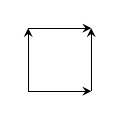
\begin{tikzpicture}[>=stealth,x=8mm,y=8mm]
\draw[->] (0,0) -- (1,0);
\draw[->] (0,1) -- (1,1);
\draw[->] (0,0) -- (0,1);
\draw[->] (1,0) -- (1,1);
\end{tikzpicture}}\endgroup}
\end{GelfandAdjacentEvidence}
\begin{GelfandAdjacentEvidence}{GELFAND-P001405}{4}


[На правом поле:]
\SourceFigure{GELFAND-P001405}{margin-arrows}{%
Здесь
\(\begin{matrix}\longrightarrow\\\longrightarrow\end{matrix}\)
гориз. морф.,\par
\(\uparrow\,\uparrow\) верт. морф.\par
(их нач. и концы — 1-морфизмы)}
\end{GelfandAdjacentEvidence}
\begin{GelfandAdjacentEvidence}{GELFAND-P001405}{5}


Можно компонировать:

\SourceFigure{GELFAND-P001405}{composable-arrow-pairs}{%
\begin{tabular}{@{}r@{\enspace}l@{\quad}l@{}}
1)&\(\longrightarrow\;\longrightarrow\)&2 гориз. морф.\\
2)&\(\begin{matrix}\uparrow\\\uparrow\end{matrix}\)&2 верт. морф.
\end{tabular}}
\end{GelfandAdjacentEvidence}
\begin{GelfandAdjacentEvidence}{GELFAND-P001405}{6}


3) квадр. двумя способами умножаются

\SourceFigure{GELFAND-P001405}{square-composition}{%
\begingroup\color{black}\GelfandFitDiagram{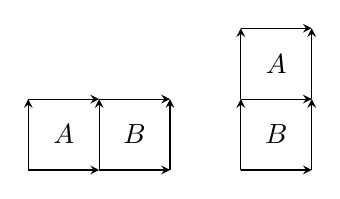
\begin{tikzpicture}[>=stealth,x=9mm,y=9mm]
\draw[->] (0,0) -- (1,0);
\draw[->] (1,0) -- (2,0);
\draw[->] (0,1) -- (1,1);
\draw[->] (1,1) -- (2,1);
\draw[->] (0,0) -- (0,1);
\draw[->] (1,0) -- (1,1);
\draw[->] (2,0) -- (2,1);
\node at (.5,.5) {\(A\)};
\node at (1.5,.5) {\(B\)};
\draw[->] (3,0) -- (4,0);
\draw[->] (3,1) -- (4,1);
\draw[->] (3,2) -- (4,2);
\draw[->] (3,0) -- (3,1);
\draw[->] (3,1) -- (3,2);
\draw[->] (4,0) -- (4,1);
\draw[->] (4,1) -- (4,2);
\node at (3.5,1.5) {\(A\)};
\node at (3.5,.5) {\(B\)};
\end{tikzpicture}}\endgroup}
\end{GelfandAdjacentEvidence}


(см. книгу Габриэля)


\Needspace{7\baselineskip}
\begin{GelfandAdjacentEvidence}{GELFAND-P001406}{1}
\SourcePage{GELFAND-P001406}{33}

\uline{Осн. нетрив. аксиома}: 2-мерн. ассоциативность

(1)
\SourceFigure{GELFAND-P001406}{interchange-diagram}{%
\begingroup\color{black}\GelfandFitDiagram{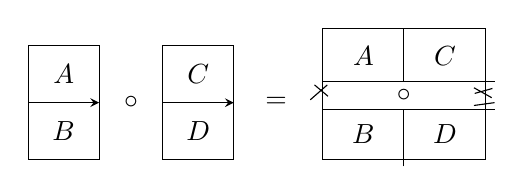
\begin{tikzpicture}[>=stealth,x=9mm,y=9mm]
  \draw (0,0) rectangle (1,1.6);
  \draw[->] (0,.8) -- (1,.8);
  \node at (.5,1.2) {\(A\)};
  \node at (.5,.4) {\(B\)};
  \node at (1.45,.8) {\(\circ\)};
  \draw (1.9,0) rectangle (2.9,1.6);
  \draw[->] (1.9,.8) -- (2.9,.8);
  \node at (2.4,1.2) {\(C\)};
  \node at (2.4,.4) {\(D\)};
  \node at (3.5,.8) {\(=\)};
  \draw (4.15,0) rectangle (6.45,1.85);
  \draw (4.15,.7) -- (6.58,.7);
  \draw (4.15,1.1) -- (6.58,1.1);
  \draw (5.3,-.1) -- (5.3,.7) (5.3,1.1) -- (5.3,1.85);
  \node at (4.73,1.46) {\(A\)};
  \node at (5.88,1.46) {\(C\)};
  \node at (4.73,.35) {\(B\)};
  \node at (5.88,.35) {\(D\)};
  \node at (5.3,.9) {\(\circ\)};
  \draw (3.98,.84) -- (4.22,1.05) (4.04,1.05) -- (4.23,.89);
  \draw (6.29,1.01) -- (6.54,.87) (6.3,.93) -- (6.55,1);
  \draw (6.29,.76) -- (6.58,.8);
\end{tikzpicture}}\endgroup
\par{\small Буква \(D\) прочитана предположительно. Штрихи по краям полосы справа не дают уверенно восстановить стрелки.}}
\end{GelfandAdjacentEvidence}
\begin{GelfandAdjacentEvidence}{GELFAND-P001406}{2}


\uline{Пример, когда не вып.}
[зачёркнуто: неразборчиво]
\uline{акс.}
[зачёркнуто: возможно, прежняя ссылка «(1)»\textsuperscript{?}]
\uline{(1)}

\Incomplete{GELFAND-P001406}{example-cancel-left}{неразборчиво}
\end{GelfandAdjacentEvidence}
\begin{GelfandAdjacentEvidence}{GELFAND-P001406}{3}

\Unclear{GELFAND-P001406}{example-cancel-right}{возможно, прежняя ссылка «(1)»}
\end{GelfandAdjacentEvidence}
\begin{GelfandAdjacentEvidence}{GELFAND-P001406}{4}



\uline{Тензоры:}

\SourceFigure{GELFAND-P001406}{tensor-horizontal}{%
\begingroup\color{black}\GelfandFitDiagram{\begin{tikzpicture}[x=9mm,y=9mm]
  \draw (0,0) rectangle (1,1);
  \node at (.5,.5) {\(A\)};
  \node at (-.24,1) {\(k\)};
  \node at (1.22,1.13) {\(\ell\)};
  \node at (-.24,-.3) {\(i\)};
  \node at (.85,-.37) {\(j\)};
  \draw (2.08,0) rectangle (3.08,1);
  \node at (2.58,.5) {\(B\)};
  \node at (1.98,1.27) {\(\ell\)};
  \node at (3.27,1.24) {\(r\)};
  \node at (1.93,-.34) {\(j\)};
  \node at (3.33,.04) {\(s\)};
  \node[anchor=west] at (3.63,.45) {свёртка};
\end{tikzpicture}}\endgroup}
\end{GelfandAdjacentEvidence}
\begin{GelfandAdjacentEvidence}{GELFAND-P001406}{5}


\[
(AB)_{ik}^{rs}=\sum A_{ij}^{k\ell} B_{js}^{\ell r}
\]
\EvidenceBlock{GELFAND-P001406}{tensor-indices}{На левой стороне \(i,k\) стоят снизу, а \(r,s\) сверху. На правой стороне индексы стоят как на рисунках \(A\) и \(B\).}{Запись в рукописи.}
\end{GelfandAdjacentEvidence}
\begin{GelfandAdjacentEvidence}{GELFAND-P001406}{6}


\SourceFigure{GELFAND-P001406}{tensor-vertical}{%
\begingroup\color{black}\GelfandFitDiagram{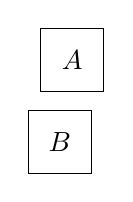
\begin{tikzpicture}[x=8mm,y=8mm]
  \draw (0,1.3) rectangle (1,2.3);
  \node at (.5,1.8) {\(A\)};
  \draw (-.2,0) rectangle (.8,1);
  \node at (.3,.5) {\(B\)};
\end{tikzpicture}}\endgroup}
\end{GelfandAdjacentEvidence}
\begin{GelfandAdjacentEvidence}{GELFAND-P001406}{7}


Аксиома (1) не будет выполнена.

\uline{Другое опр.} (\uline{М. Концевич}) (конкурирующее)

\SourceFigure{GELFAND-P001406}{parallel-morphisms}{%
\begingroup\color{black}\GelfandFitDiagram{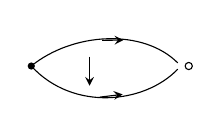
\begin{tikzpicture}[>=stealth,x=10mm,y=10mm]
  \fill (0,0) circle (1.3pt);
  \draw (2,0) circle (1.3pt);
  \draw (0,0) .. controls (.53,.43) and (1.42,.48) .. (1.86,.04);
  \draw[->] (.9,.326) -- (1.17,.33);
  \draw (0,0) .. controls (.53,-.58) and (1.44,-.48) .. (1.86,-.04);
  \draw[->] (.87,-.395) -- (1.16,-.36);
  \draw[->] (.74,.12) -- (.74,-.25);
\end{tikzpicture}}\endgroup
\par морфизмы между морф. с одинаков. концами.}
\end{GelfandAdjacentEvidence}
\begin{GelfandAdjacentEvidence}{GELFAND-P001406}{8}


\uline{Пример:} \(Cat\) (категория категорий; есть морфизм функторов)

Это частный случай предыдущего (стягиваем верт. стрелки).

\uline{И. М. Г.}

\SourceFigure{GELFAND-P001406}{boundary-diagram}{%
\begingroup\color{black}\GelfandFitDiagram{\begin{tikzpicture}[>=stealth,x=11mm,y=11mm]
  \draw[thick] (0,0) rectangle (1.55,1.24);
  \draw[->] (.05,.94) -- (1.43,1.03);
  \draw[->] (.08,.16) -- (1.48,.29);
  \draw[->] (.18,.03) -- (.29,1.15);
  \draw[->] (.33,.03) -- (.47,1.16);
  \node at (1,.59) {\(\Delta u=0\)};
  \node[anchor=east] at (-.1,.22) {\(u\) и \(\dfrac{\partial u}{\partial n}\)};
  \node[anchor=east] at (-.55,.86) {св.\textsuperscript{?}};
\end{tikzpicture}}\endgroup
\par гран. условия
\par{\small Над \(u\) видны открытый и высокий петлеобразный штрихи. Сокращение предположительно читается «св.».}}
\end{GelfandAdjacentEvidence}


Просьба к Келдышу — Ченцову — Гельфанду

\uuline{К.} Высшие фунд. гр.
\(X_0\subset X_1\subset X\) — топ. пр-во

объекты — точки \(x\in X_0\)

морф.
\(\bigl(\underset{\text{отрезок}}{I},\partial I\bigr)
\longrightarrow(X_1,X_0)\)
\qquad гомотопные \((\bmod\,\partial I)\) счит. эквив.

биморфизмы
\((I^2,\partial I^2)\longrightarrow(X,X_1)\)
\qquad \((\bmod\,\text{\uline{гомотопии}})\)


\Needspace{7\baselineskip}
\begin{GelfandAdjacentEvidence}{GELFAND-P001407}{1}
\SourcePage{GELFAND-P001407}{44}

\uuline{23/XI-87 г.}\qquad \uline{Сем. Гельфанда.}

\uline{Бейлинсон} (продолжение)

\uline{Производные категории.}

(1) \uline{Лемма:}
\SourceFigure{GELFAND-P001407}{lemma-roofs}{%
\begingroup\color{black}\GelfandFitDiagram{\begin{tikzpicture}[>=stealth,x=8mm,y=8mm,font=\small]
  \node (x) at (0,1.35) {\(X^\bullet\)};
  \node (y) at (1.88,1.35) {\(Y^\bullet\)};
  \node (z) at (.89,0) {\(Z^\bullet\)};
  \draw[->] (z) -- (x) node[midway,below left,align=left,font=\scriptsize] {квази-\\изом.};
  \draw[->] (z) -- (y);
  \node at (2.65,.7) {\(\Rightarrow\)};
  \node at (3.47,.7) {\(\exists\)};
  \node (xx) at (4.45,.03) {\(X^\bullet\)};
  \node (yy) at (6.7,.03) {\(Y^\bullet\)};
  \node (zz) at (5.58,1.35) {\(Z'^\bullet\)};
  \draw[->] (xx) -- (zz) node[midway,above left,font=\scriptsize] {квазиизом.};
  \draw[->] (yy) -- (zz);
\end{tikzpicture}}\endgroup}
\end{GelfandAdjacentEvidence}
\begin{GelfandAdjacentEvidence}{GELFAND-P001407}{2}


Лемма док. с пом. конструкции конуса отображения.

\uline{Напоминание:}

\(\mathcal A\) — аб. категория
\SourceFigure{GELFAND-P001407}{category-sequence}{%
\(\begin{array}{@{}ccccc@{}}
C(\mathcal A)&\longrightarrow&K(\mathcal A)&\longrightarrow&D(\mathcal A)\\
\text{\scriptsize комплексы}&&
\substack{\text{гомотоп.}\\\text{катег.}\\\text{комплексов}}&&
\substack{\text{производная}\\\text{категория}}
\end{array}\)}
\end{GelfandAdjacentEvidence}
\begin{GelfandAdjacentEvidence}{GELFAND-P001407}{3}

[Справа:] (объекты всюду суть комплексы)

\(f:X^\bullet\to Y^\bullet\) гомотопно \(0\), если
\(\exists g^i:X^i\to Y^{i-1}\),
\[
f^i=dg^i+g^{i+1}d.
\]

\(D(\mathcal A)\) — это \(K(\mathcal A)\) с обращенными
\uline{квазиизоморфизмами}
(морф., индуц. изоморфизм когомологий)

Морфизм из \(X^\bullet\) в \(Y^\bullet\) — это диаграмма в \(K(\mathcal A)\)

(2)
\SourceFigure{GELFAND-P001407}{morphism-roof}{%
\begingroup\color{black}\GelfandFitDiagram{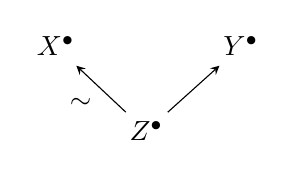
\begin{tikzpicture}[>=stealth,x=10mm,y=9mm]
  \node (x) at (0,1.2) {\(X^\bullet\)};
  \node (y) at (2.35,1.2) {\(Y^\bullet\)};
  \node (z) at (1.15,0) {\(Z^\bullet\)};
  \draw[->] (z) -- (x) node[midway,below left] {\(\sim\)};
  \draw[->] (z) -- (y);
\end{tikzpicture}}\endgroup}
\end{GelfandAdjacentEvidence}
\begin{GelfandAdjacentEvidence}{GELFAND-P001407}{4}

(левая стрелка — квазиизоморфизм)

точнее, класс эквивал. таких диаграмм: диагр. (2) эквивалентна диаграмме, полученной с пом. любого квазиизоморфизма
\(\chi:Z'^\bullet\to Z^\bullet\)

(3)
\SourceFigure{GELFAND-P001407}{refinement-roofs}{%
\begingroup\color{black}\GelfandFitDiagram{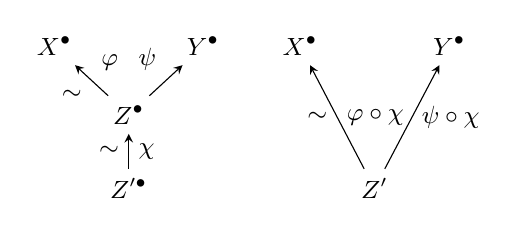
\begin{tikzpicture}[>=stealth,x=8mm,y=8mm,font=\small]
  \node (x) at (0,1.93) {\(X^\bullet\)};
  \node (y) at (2.36,1.93) {\(Y^\bullet\)};
  \node (z) at (1.18,.84) {\(Z^\bullet\)};
  \node (zp) at (1.18,-.33) {\(Z'^\bullet\)};
  \draw[->] (z) -- (x) node[midway,above right] {\(\varphi\)}
    node[midway,below left] {\(\sim\)};
  \draw[->] (z) -- (y) node[midway,above left] {\(\psi\)};
  \draw[->] (zp) -- (z) node[midway,right] {\(\chi\)}
    node[midway,left] {\(\sim\)};
  \node (xx) at (3.9,1.93) {\(X^\bullet\)};
  \node (yy) at (6.27,1.93) {\(Y^\bullet\)};
  \node (zz) at (5.08,-.33) {\(Z'\)};
  \draw[->] (zz) -- (xx) node[midway,right] {\(\varphi\circ\chi\)}
    node[midway,left] {\(\sim\)};
  \draw[->] (zz) -- (yy) node[midway,right] {\(\psi\circ\chi\)};
\end{tikzpicture}}\endgroup}
\end{GelfandAdjacentEvidence}
\begin{GelfandAdjacentEvidence}{GELFAND-P001407}{5}


(это отношение продолжается до наименьшего содержащего его отношения эквивалентности)

Конус морфизма и точные треугольники были определены [зачёркнуто: неразборчиво] ещё.
\Unclear{GELFAND-P001407}{last-line-cancellation}{Короткая зачёркнутая запись перед «ещё» неразборчива.}
\end{GelfandAdjacentEvidence}



\Needspace{7\baselineskip}
\begin{GelfandAdjacentEvidence}{GELFAND-P001408}{1}
\SourcePage{GELFAND-P001408}{unlabelled}

\uuline{И. Захаревич}
[зачёркнуто: неразборчиво]
\uline{Импровизация о хаосе.}

\Incomplete{GELFAND-P001408}{cancelled-title}{неразборчиво}
\end{GelfandAdjacentEvidence}
\begin{GelfandAdjacentEvidence}{GELFAND-P001408}{2}



\Unclear{GELFAND-P001408}{title-preposition}{Предлог в заглавии, вероятно, «о». Незамкнутый штрих похож также на «с».}
\end{GelfandAdjacentEvidence}
\begin{GelfandAdjacentEvidence}{GELFAND-P001408}{3}


\uline{Примеры}

\(1^\circ\). Видимо, есть морфизм из одного примера в другой.
\[
M=(\mathbb{Z}/2\mathbb{Z})^{\mathbb{Z}}
\qquad\text{(беск. в обе стороны послед.)}
\]
\(T:M\to M\). На \(M\) станд. топология (кантор. мн-во).
\[
a_i\to a_{i-1}\qquad\text{(преобр. сдвига; преобр. Бернулли)}
\]
Рассм. итерации: \(T^N\).

На \(M\) есть мера. Преобр. пекаря совпадает с этим
[вставлено над строкой: (с точн. до меры \(0\))]
[зачёркнуто: продолжение на двух строках].
\Unclear{GELFAND-P001408}{baker-cancellations}{Верхняя строка похожа на «если брать», нижняя — на «не \(\mathbb{Z}\), вместо \(\mathbb{Z}\)».}
\end{GelfandAdjacentEvidence}
\begin{GelfandAdjacentEvidence}{GELFAND-P001408}{4}


\SourceFigure{GELFAND-P001408}{baker-axes}{%
\begingroup\color{black}\GelfandFitDiagram{\begin{tikzpicture}[>=stealth,x=24mm,y=24mm,font=\small]
  \draw[->] (0,0) -- (2.13,0);
  \draw[->] (0,0) -- (0,1.32);
  \draw (0,1) -- (1,1) -- (1,0);
  \draw (2.02,0) -- (2.02,.51);
  \draw[dashed] (.03,.49) -- (2.07,.54);
  \foreach \x in {.08,.3,.68,1.1,1.42,1.72} {
    \draw[thin] (\x,.12) -- ++(.14,.22);
  }
  \draw[->] (1.39,.34) .. controls (1.52,.81) and (1.24,.88) .. (.58,.78);
  \node[below left] at (0,0) {\(0\)};
  \node[left] at (0,1) {\(1\)};
  \node[below] at (1,0) {\(1\)};
\end{tikzpicture}}\endgroup}
\end{GelfandAdjacentEvidence}
\begin{GelfandAdjacentEvidence}{GELFAND-P001408}{5}


\SourceFigure{GELFAND-P001408}{baker-sequence}{%
\begingroup\color{black}\GelfandFitDiagram{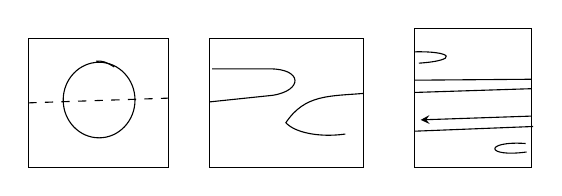
\begin{tikzpicture}[>=stealth,x=12mm,y=12mm]
  \draw (0,0) rectangle (1.48,1.36);
  \draw (.75,.71) ellipse (.38 and .4);
  \draw[dashed] (0,.68) -- (1.48,.73);
  \draw (.72,1.12) .. controls (.78,1.13) and (.83,1.11) .. (.91,1.06);
  \begin{scope}[xshift=23mm]
    \draw (0,0) rectangle (1.63,1.36);
    \draw (.03,1.04) -- (.64,1.04)
      .. controls (.99,1.04) and (.99,.81) .. (.67,.76)
      -- (0,.69);
    \draw (1.63,.78) .. controls (1.27,.75) and (1.01,.77) .. (.81,.47)
      .. controls (.9,.37) and (1.15,.31) .. (1.44,.35);
  \end{scope}
  \begin{scope}[xshift=49mm]
    \draw (0,0) rectangle (1.24,1.47);
    \draw (0,1.22) .. controls (.41,1.23) and (.48,1.13) .. (.05,1.1);
    \draw (0,.92) -- (1.24,.93) (0,.79) -- (1.24,.83);
    \draw[<-] (.07,.5) -- (1.24,.54);
    \draw (0,.38) -- (1.26,.43);
    \draw (1.18,.25) .. controls (.74,.28) and (.75,.1) .. (1.19,.16);
  \end{scope}
\end{tikzpicture}}\endgroup
\par и т. д.
\par{\small Мелкие штрихи у кривых первого и третьего рисунков не дают уверенно прочитать направление.}}
\end{GelfandAdjacentEvidence}
\begin{GelfandAdjacentEvidence}{GELFAND-P001408}{6}


\uline{Соответствие}: записать коорд. точки квадрата в двоичной системе и взять \(1\) цифру — налево, другую — направо.

В каком смысле это хаос

Рассм. \(T^k x,\ k\le 0\) — пусть это известно (с точн. до \(1\) мм).
\[
T^k x,\qquad k>0
\]
за конечное время вся эта информ. потеряется.

\(2^\circ\). \uline{Гиперболич. преобразование}: геодезич. потоки на мн-зиях отриц. кривизны.
\EvidenceBlock{GELFAND-P001408}{manifold-abbreviation}{Сокращение «мн-зиях».}{Запись в рукописи.}
\end{GelfandAdjacentEvidence}
\begin{GelfandAdjacentEvidence}{GELFAND-P001408}{7}


\SourceFigure{GELFAND-P001408}{hyperbolic-surface}{%
\begingroup\color{black}\GelfandFitDiagram{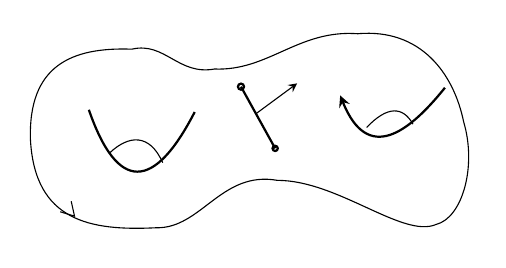
\begin{tikzpicture}[>=stealth,x=14mm,y=14mm]
  \draw (0,.8) .. controls (-.02,1.47) and (.37,1.64) .. (.92,1.62)
    .. controls (1.22,1.69) and (1.34,1.38) .. (1.67,1.44)
    .. controls (2.16,1.42) and (2.43,1.8) .. (2.97,1.76)
    .. controls (3.54,1.81) and (3.84,1.4) .. (3.93,.96)
    .. controls (4.05,.56) and (3.92,.09) .. (3.68,.03)
    .. controls (3.38,-.1) and (2.79,.43) .. (2.24,.43)
    .. controls (1.73,.52) and (1.55,-.01) .. (1.14,0)
    .. controls (.54,-.03) and (.04,.06) .. (0,.8);
  \draw[thick] (.53,1.07) .. controls (.79,.32) and (1.12,.33) .. (1.49,1.05);
  \draw (.72,.68) .. controls (.89,.84) and (1.08,.86) .. (1.2,.59);
  \draw (.37,.24) -- (.4,.105) -- (.27,.145);
  \draw[thick] (1.91,1.28) -- (2.22,.72);
  \draw[->] (2.04,1.03) -- (2.42,1.31);
  \draw[thick] (1.91,1.28) circle (1.1pt) (2.22,.72) circle (.95pt);
  \draw[thick,<-] (2.81,1.2) .. controls (3.06,.58) and (3.43,.86) .. (3.76,1.27);
  \draw (3.05,.91) .. controls (3.24,1.11) and (3.38,1.1) .. (3.47,.94);
\end{tikzpicture}}\endgroup
\par{\small Стрелка у средней ветви направлена вправо-вверх. Штрих у левого края контура и мелкие метки на средней линии читаются неуверенно.}}
\end{GelfandAdjacentEvidence}



\Needspace{7\baselineskip}
\begin{GelfandAdjacentEvidence}{GELFAND-P001409}{1}
\SourcePage{GELFAND-P001409}{45}

\uuline{Г. Маргулис.}\qquad \uline{Итерации отображений компл. плоскости.}

Рассм. преобр. \(z\to P(z)\), \(P\) — многочлен

(более общо — рац. ф-я)

\(\deg P=1\) [зачёркнуто: неразборчиво] неинтересный случай
\Incomplete{GELFAND-P001409}{degree-one-cancellation}{Короткая запись после \(\deg P=1\) неразборчива.}
\end{GelfandAdjacentEvidence}
\begin{GelfandAdjacentEvidence}{GELFAND-P001409}{2}


\begin{equation*}
z\mapsto az+b \tag{1}
\end{equation*}

\uline{Итерации}:
\[
z_{i+1}=P(z_i)
\]
\(\lvert a\rvert>1\Rightarrow\) одна неподв. точка;

\(\lvert a\rvert=1\Rightarrow\) всё разбив. на инвар. окружности, на к-рых поворот.
\EvidenceBlock{GELFAND-P001409}{unit-modulus-claim}{В рукописи написано \(\lvert a\rvert=1\).}{Запись в рукописи.}
\end{GelfandAdjacentEvidence}
\begin{GelfandAdjacentEvidence}{GELFAND-P001409}{3}


\SourceFigure{GELFAND-P001409}{invariant-circles}{%
\begingroup\color{black}\GelfandFitDiagram{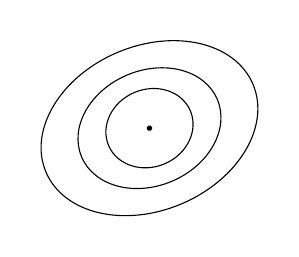
\begin{tikzpicture}[x=12mm,y=12mm,rotate=23]
  \draw (0,0) ellipse (1.19 and .87);
  \draw (0,0) ellipse (.78 and .61);
  \draw (0,0) ellipse (.47 and .41);
  \fill (0,0) circle (1pt);
\end{tikzpicture}}\endgroup}
\end{GelfandAdjacentEvidence}
\begin{GelfandAdjacentEvidence}{GELFAND-P001409}{4}


\uuline{И. М. Г.}: 1) вопрос о том, когда преобраз. окружности диффеоморфно повороту, нетривиален: Данжуа, Арнольд, Herman

2) Что такое представление дискретной бескон. группы?

Нет удовлетв. ответа.

Фон Неймановская теор. не эстетична.

На окружности возникает хаос.

\uline{Гипотеза}: если работать с мн-вами промежуточной хаусдорфовой размерности, то нек-рая классика восстановится!!

\uline{Вопрос для школьников}: покрываем \(n\)-е рац. число интервалом длины \(\varepsilon/2^n\). Привести пример числа, к-рое не будет покрыто.

\uline{Задача}: найти хаусд. размерность канторовского соверш. мн-ва.

\tikz[baseline=(emphasis.base)]\node[draw,circle,inner sep=2pt] (emphasis) {!};
\uuline{Задача}. \uwave{Построить теорию предст. дискр. групп на ф-ях на мн-вах промежут. хаусд. размерности.}

Для начала посмотреть физику — теор. струн и т. д.

\uuline{Г. М.}:
\(z\to z^2\)
\qquad \(\lvert z\rvert=1\) перех. в себя

\SourceFigure{GELFAND-P001409}{squaring-dynamics}{%
\begingroup\color{black}\GelfandFitDiagram{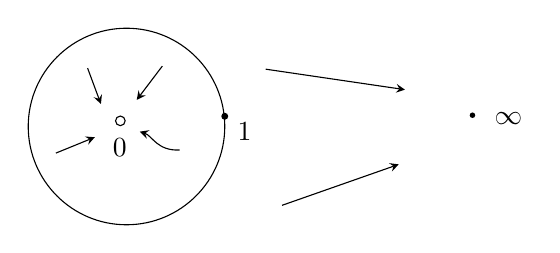
\begin{tikzpicture}[>=stealth,x=13mm,y=13mm]
  \draw (0,0) circle (.96);
  \draw (-.06,.055) circle (.047);
  \node[below] at (-.065,-.025) {\(0\)};
  \fill (.96,.1) circle (1.25pt);
  \node[right] at (.99,-.045) {\(1\)};
  \draw[->] (-.38,.57) -- (-.25,.22);
  \draw[->] (.35,.59) -- (.1,.26);
  \draw[->] (.52,-.23) .. controls (.3,-.24) and (.25,-.09) .. (.13,-.05);
  \draw[->] (-.69,-.26) -- (-.31,-.105);
  \draw[->] (1.36,.56) -- (2.72,.36);
  \draw[->] (1.52,-.77) -- (2.66,-.37);
  \fill (3.38,.11) circle (1pt);
  \node[right] at (3.5,.08) {\(\infty\)};
\end{tikzpicture}}\endgroup}
\end{GelfandAdjacentEvidence}


на окр. — аналог преобр. пекаря (одностороннего)


\Needspace{7\baselineskip}
\begin{GelfandAdjacentEvidence}{GELFAND-P001410}{1}
\SourcePage{GELFAND-P001410}{unlabelled}

\[
f_n=\underbrace{f\circ f\circ\cdots\circ f}_{n\ \text{раз}}
\]

\uline{Опр.}

\(U\) —
[зачёркнуто: мн-во; вписано над строкой: \uline{окр.}]
нормальности; если \(\left.f_n\right|_U\) — компактное мн-во

(норм. сем-во анал. ф-й)
\EvidenceBlock{GELFAND-P001410}{definition-cancellation}{«мн-во» зачёркнуто, над ним вписано «окр.».}{Запись в рукописи.}
\end{GelfandAdjacentEvidence}
\begin{GelfandAdjacentEvidence}{GELFAND-P001410}{2}


[На отдельной короткой строке зачёркнуто:]
\Incomplete{GELFAND-P001410}{isolated-cancellation}{неразборчиво}
\end{GelfandAdjacentEvidence}
\begin{GelfandAdjacentEvidence}{GELFAND-P001410}{3}


\uline{Мн-во норм.} [вписано над строкой: \(X\)] сост. из точек \(x\),
для к-рых \(\exists\) окр. \(U\) ---
[зачёркнуто: неразборчиво] окр. нормальности
\Incomplete{GELFAND-P001410}{normality-cancellation}{Зачёркнутая запись перед «окр. нормальности» неразборчива.}
\end{GelfandAdjacentEvidence}
\begin{GelfandAdjacentEvidence}{GELFAND-P001410}{4}


[Под \uline{Мн-во норм.}: (оно открыто)]

Дополнение к мн-ву нормальности — \uwave{мн-во Жюлиа}.

(оно замкнуто)

Мн-во норм. может быть пусто

\[
X=X_1\cup\cdots\cup X_n\cup\cdots
\]
(связные компоненты) мн-ва нормальности

[зачёркнуто под этой подписью: неразборчиво]
\Incomplete{GELFAND-P001410}{components-cancellation}{Под подписью видны отдельные буквы, но запись целиком не читается.}
\end{GelfandAdjacentEvidence}
\begin{GelfandAdjacentEvidence}{GELFAND-P001410}{5}


\[
\begin{aligned}
f:(\text{св. компон.})&\to(\text{св. компоненты})\\
X_i&\mapsto X_{j(i)}
\end{aligned}
\]

\uwave{Sullivan} доказал, что в возникающем [зачёркнуто: неразборчиво]
преобр. дискр. мн-ва (счётн. или конечного)
\Incomplete{GELFAND-P001410}{sullivan-cancellation}{Зачёркнутая запись перед «преобр.» неразборчива.}
\end{GelfandAdjacentEvidence}
\begin{GelfandAdjacentEvidence}{GELFAND-P001410}{6}


а) каждая орбита стабилизируется,

б) мн-во неподв. точек конечно.

\uline{Идея док-ва.} Пусть есть беск. орбита

\SourceFigure{GELFAND-P001410}{orbit-diagram}{%
\begingroup\color{black}\GelfandFitDiagram{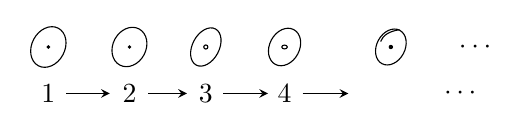
\begin{tikzpicture}[>=stealth,x=10mm,y=10mm]
  \foreach \x/\radiusX/\radiusY in {0/.21/.27,1.03/.21/.26,2/.17/.26,3/.19/.25,4.35/.18/.24} {
    \begin{scope}[shift={(\x,0)},rotate=-28]
      \draw (0,0) ellipse[x radius={\radiusX},y radius={\radiusY}];
    \end{scope}
  }
  \fill (0,0) circle (.7pt) (1.03,0) circle (.7pt) (4.35,0) circle (.8pt);
  \draw (2,0) circle (.75pt) (3,0) ellipse (1.0pt and .7pt);
  \draw (4.22,.07) .. controls (4.25,.15) and (4.33,.2) .. (4.46,.22);
  \node at (5.42,0) {\(\cdots\)};
  \foreach \x/\digit in {0/1,1.03/2,2/3,3/4} {
    \node at (\x,-.59) {\(\digit\)};
  }
  \foreach \from/\to in {.23/.78,1.27/1.76,2.22/2.79,3.23/3.81} {
    \draw[->] (\from,-.59) -- (\to,-.59);
  }
  \node at (5.23,-.59) {\(\cdots\)};
\end{tikzpicture}}\endgroup}
\end{GelfandAdjacentEvidence}
\begin{GelfandAdjacentEvidence}{GELFAND-P001410}{7}


Сделаем замену конф. [зачёркнуто: возможно, «преобр.»] структуры, чтобы преобр. осталось конформным.
\Unclear{GELFAND-P001410}{structure-cancellation}{Зачёркнутое сокращение предположительно читается как «преобр.».}
\end{GelfandAdjacentEvidence}
\begin{GelfandAdjacentEvidence}{GELFAND-P001410}{8}


\uline{Задача:}

\SourceFigure{GELFAND-P001410}{circle-packing}{%
\begingroup\color{black}\GelfandFitDiagram{\begin{tikzpicture}[>=stealth,x=11mm,y=11mm]
  \draw[thick] (0,0) rectangle (3.02,2.72);
  \draw (.86,1.94) ellipse (.86 and .78);
  \draw (2.31,1.97) ellipse (.7 and .74);
  \draw[rotate around={23:(.78,.57)}] (.78,.57) ellipse (.62 and .53);
  \draw[rotate around={14:(2.16,.59)}] (2.16,.59) ellipse (.82 and .58);
  \draw[rotate around={31:(1.57,1.28)}] (1.57,1.28) ellipse (.31 and .23);
  \draw (.16,1.16) ellipse (.16 and .22);
  \draw (2.91,1.28) ellipse (.11 and .15);
  \draw (.14,2.54) ellipse (.13 and .16);
  \draw (1.77,2.63) ellipse (.13 and .09);
  \draw (2.95,2.63) ellipse (.066 and .083);
  \draw (1.32,.12) ellipse (.12 and .11);
  \draw (2.93,.13) ellipse (.087 and .12);
  \draw (0,.07) .. controls (.14,.04) and (.15,.12) .. (.16,.21) (.77,1.17) .. controls (.86,1.29) and (.99,1.30) .. (1.08,1.19);
  \draw[<-] (3.42,1.43) -- (4.25,1.43);
  \node[right] at (4.27,1.43) {вписываем};
\end{tikzpicture}}\endgroup
\par{\small Касания и отдельные мелкие дуги у границы показаны приблизительно.}}
\end{GelfandAdjacentEvidence}


1) Док., что остаток имеет меру \(0\)

2) Док., что остаток имеет хаусд. размерность \(<2\).


\Needspace{7\baselineskip}
\begin{GelfandAdjacentEvidence}{GELFAND-P001411}{1}
\SourcePage{GELFAND-P001411}{46}

\uuline{И. М. Гельфанд}. \uline{Матроиды.}

В \(K\)-мерном пр-ве рассм. \(n\) векторов;
занумеруем их и составим список: какие лин. завис., а какие — нет.

Задание этого списка — \uwave{матроид}.

Какие условия на этот список?

\uline{Пример}:
[Зачёркнуто: неразборчиво]
\Incomplete{GELFAND-P001411}{example-cancelled}{Запись после «Пример» неразборчива.}
\end{GelfandAdjacentEvidence}
\begin{GelfandAdjacentEvidence}{GELFAND-P001411}{2}


\SourceFigure{GELFAND-P001411}{fano-diagram}{%
\begingroup\color{black}\GelfandFitDiagram{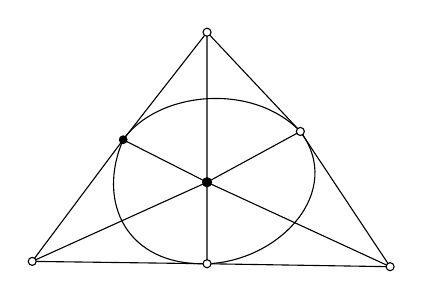
\begin{tikzpicture}[x=15mm,y=15mm]
  \coordinate (a) at (0,1.96);
  \coordinate (b) at (-1.48,.02);
  \coordinate (c) at (1.55,-.025);
  \coordinate (d) at (-.71,1.05);
  \coordinate (e) at (.79,1.12);
  \coordinate (f) at (0,0);
  \coordinate (g) at (0,.69);
  \draw (a)--(d)--(b)--(f)--(c)--(e)--cycle;
  \draw (a)--(g)--(f) (b)--(g)--(e) (d)--(g)--(c);
  \draw (d) .. controls (-.43,1.45) and (.37,1.55) .. (e)
    .. controls (1.17,.61) and (.61,.02) .. (f)
    .. controls (-.68,-.02) and (-.94,.52) .. (d);
  \foreach \point in {a,b,c,e,f} {
    \draw[fill=white] (\point) circle (1.45pt);
  }
  \fill (d) circle (1.6pt) (g) circle (1.85pt);
\end{tikzpicture}}\endgroup}
\end{GelfandAdjacentEvidence}
\begin{GelfandAdjacentEvidence}{GELFAND-P001411}{3}


если 3 точки лежат на одной линии, то векторы линейно зависимы.

Всё пр-во 3-мерно (нет 4-х лин. независимых)

(1) \uline{Задача}: 1) док., что над \(\mathbb R\) и \(\mathbb C\)
таких векторов нет!

2) над \(\mathbb Z/2\mathbb Z\) такие векторы есть.

(все ненулевые векторы у \((\mathbb Z/2\mathbb Z)^3\)!)

\uline{Общая} (\uline{нереш. задача}): какие матроиды реализуются
а) над \(\mathbb R\)
б) над \(\mathbb C\).?

\uwave{Решена задача}: какие матроиды реализ. над \(\forall\) полем?

\uline{В книжке Рота} э\textsuperscript{?}\ldots
[Справа: см. книге\textsuperscript{?} \uwave{Айгнера} (?)]
имеется 15 различных эквив. опр. матроида.

\Unclear{GELFAND-P001411}{book-after-rota}{После «Рота» видны изогнутый штрих, похожий на «э», и точки. Штрих соединён с подчёркиванием.}
\end{GelfandAdjacentEvidence}
\begin{GelfandAdjacentEvidence}{GELFAND-P001411}{4}

\Unclear{GELFAND-P001411}{book-overwritten-noun}{Первое слово после «см.» исправлено и читается предположительно как «книге» или «книжке».}
\end{GelfandAdjacentEvidence}
\begin{GelfandAdjacentEvidence}{GELFAND-P001411}{5}


(2) \uline{Аксиоматика.}

Выделены подмн-ва, \uwave{называемые базисами}

\(B_1,B_2\) — 2 базиса

\[
y\in B_2,\ y\notin B_1\Rightarrow\exists x\in B_1;\qquad
(B_1\setminus x)\cup y,\quad (B_2\setminus y)\cup x
\]
— базисы [Зачёркнуто: запись между двумя выражениями]
\Incomplete{GELFAND-P001411}{basis-exchange-cancelled}{Запись после \((B_1\setminus x)\cup y\) зачёркнута и неразборчива.}
\end{GelfandAdjacentEvidence}
\begin{GelfandAdjacentEvidence}{GELFAND-P001411}{6}


\uwave{Упр. из лин. алгебры}: проверить для мн-ва векторов в лин. пр-ве.

(3) \uwave{Биматроид}: рассм. матрицу; из неё опр. 2 матроида — по столбцам и строкам

\(S\) и \(T\)

Другое понятие: выписать все миноры \(\ne0\)

Биматроид: набор подмн-в с одинак. числом элементов.

(4) [Зачёркнуто: неразборчиво] \uline{Задача}: указать аксиомы для биматроида.
\Incomplete{GELFAND-P001411}{problem-four-cancelled}{Короткая запись перед «Задача» неразборчива.}
\end{GelfandAdjacentEvidence}



\Needspace{7\baselineskip}
\begin{GelfandAdjacentEvidence}{GELFAND-P001412}{1}
\SourcePage{GELFAND-P001412}{unlabelled}

(5) \uline{Задача}: как понятие биматроида из
[Зачёркнуто: неразборчиво] Гельфанда — Сергановой (УМН)
связано с Кунтом\textsuperscript{?}
\Incomplete{GELFAND-P001412}{top-cancelled}{Зачёркнутая запись после «из» неразборчива.}
\end{GelfandAdjacentEvidence}
\begin{GelfandAdjacentEvidence}{GELFAND-P001412}{2}

\Unclear{GELFAND-P001412}{knuth-name}{Фамилия предположительно читается как «Кунтом». Округлый штрих перед «т» читается неуверенно.}
\end{GelfandAdjacentEvidence}
\begin{GelfandAdjacentEvidence}{GELFAND-P001412}{3}


\uline{Задача}: доказать, что

\[
\begin{aligned}
\text{(6)}\quad [x_1,\ldots,x_d][y_1,\ldots,y_d]
 &= \sum(-1)^{d-i}[y_1,x_2,\ldots,x_d]\\
 &\qquad [y_1,\ldots,y_{i-1},x_i,y_{i+1},\ldots,y_d]
\end{aligned}
\]
\EvidenceBlock{GELFAND-P001412}{determinant-formula-source}{Знак \( (-1)^{d-i} \) и индексы \(y_1\), \(x_i\) переданы по рукописи.}{Запись в рукописи.}
\end{GelfandAdjacentEvidence}
\begin{GelfandAdjacentEvidence}{GELFAND-P001412}{4}


\([x_1,\ldots,x_d]\) — детерминант, постр. по вект.

(7) \uline{Замеч.}: если \([x_1,\ldots,x_d]\), \([y_1,\ldots,y_d]\)
— базисы, то справа есть ненулевое слагаемое — это и даёт аксиому замены (3)
\EvidenceBlock{GELFAND-P001412}{basis-axiom-reference}{Ссылка (3) по рукописи.}{Запись в рукописи.}
\end{GelfandAdjacentEvidence}
\begin{GelfandAdjacentEvidence}{GELFAND-P001412}{5}


(8) \uline{Задача} (нудная). Цепь сизигий по Гильберту:
\[
(\text{кольцо})\longmapsto
\underset{\text{— детерминанты}}{(\text{образующие})}
\longmapsto (\text{соотн. между образующими})
\]
\Unclear{GELFAND-P001412}{overwritten-eight}{Видимая цифра читается как 8. Первоначальная запись под ней неразборчива.}
\end{GelfandAdjacentEvidence}
\begin{GelfandAdjacentEvidence}{GELFAND-P001412}{6}


(9) (\uline{Утв.}: (6) — все соотн. между образующими)

(10) а) Написать всю цепочку!

б) Дискретизовать (комбинат. соотн. написать) всей цепочки.

(11) \uline{Задача}. Биматроид — список миноров \(\longrightarrow\)
[Зачёркнуто: неразборчиво] 2 матроида (стр. и столбцы)
\Incomplete{GELFAND-P001412}{problem-eleven-cancelled}{Зачёркнутая запись перед «2 матроида» неразборчива.}
\end{GelfandAdjacentEvidence}
\begin{GelfandAdjacentEvidence}{GELFAND-P001412}{7}


По 2-м матроидам строится биматроид

\SourceFigure{GELFAND-P001412}{basis-grid}{%
\begingroup\color{black}\GelfandFitDiagram{\begin{tikzpicture}[x=8mm,y=8mm]
  \foreach \x in {0,.4,.8,1.2} {
    \draw (\x,-.16) -- (\x,1.36);
  }
  \foreach \y in {0,.4,.8,1.2} {
    \draw (-.22,\y) -- (1.55,\y);
  }
  \draw[decorate,decoration={brace,amplitude=3pt}]
    (-.37,-.18) -- (-.37,1.38) node[midway,left=4pt]{баз\textsuperscript{?}};
  \draw[decorate,decoration={brace,amplitude=3pt}]
    (1.55,-.39) -- (-.22,-.39) node[midway,below=4pt]{база};
  \draw[<-] (1.76,.48) -- (3.18,.48);
\end{tikzpicture}}\endgroup\par{\small Под решёткой написано «база». Конец подписи слева неясен.}}
\end{GelfandAdjacentEvidence}
\begin{GelfandAdjacentEvidence}{GELFAND-P001412}{8}


по опр. \uwave{база}.
\EvidenceBlock{GELFAND-P001412}{basis-construction-word}{Слово после «по опр.» подчёркнуто и читается как «база».}{Запись в рукописи.}
\end{GelfandAdjacentEvidence}


Но это не обязательно.

В биматроиде больше информации.

Какова доп. информация в биматроиде?

Это важное когомологич. понятие.

\uline{Замеч.}. Алгебр. топология — маленький остров в привычной комбинат. технике.


\Needspace{7\baselineskip}
\SourcePage{GELFAND-P001413}{unlabelled}

\uuline{30/XI-87 г.}\qquad \uline{Сем. Гельфанда.}

\uline{И. М. Гельфанд.} Задача: найти характеры симметрической группы.

(по следам Фробениуса).

\uline{О раб.} \uwave{Керова}: «\uline{Реализация предст. алгебры Геке} и т. д.»

Подсказка: это характеры симм. группы.

Алгебра Геке — алгебра с образующими \(\{e_k\}\) [над строкой: \(k=1,\ldots,N-1\)] и соотношениями
\[
\text{(1)}\quad
\left\{\begin{aligned}
e_k e_{k+1}e_k-\tau e_k&=e_{k+1}e_ke_{k+1}-\tau e_{k+1}\\
e_{k+j}e_k&=e_ke_{k+j},\quad j\geqslant 2,\\
e_k^2&=e_k
\end{aligned}\right.
\]
Другие образующие
\[
\text{(2)}\quad \sigma_k=(q+1)e_k-1,\qquad \tau=\frac{q}{(q+1)^2}
\]
Эта алг. обозначается \(H_N(q)\).

\uline{Упражнение}: записать соотношения на \(\sigma_k\).

(3) При \(q=1\) (или \(\tau=\frac14\)) получается групповая алгебра симм. группы.

(4) \uline{Задача}: \(\dim H_N(q)=N!\)

\begin{GelfandAdjacentEvidence}{GELFAND-P001413}{1}
[На левом поле: \textcircled{!}]
В работе Типпера и Джеймса

Proc. London Math. Soc.\qquad 1986, v. 52, p. 20--52

рекомендуется!!

\EvidenceBlock{GELFAND-P001413}{citation-name}{В рукописи написано «Типпера». В указанном издании автора зовут R. Dipper.}{Запись в рукописи.}
\end{GelfandAdjacentEvidence}
\begin{GelfandAdjacentEvidence}{GELFAND-P001413}{2}


док., что теория предст. \(H_N(q)\) аналогична теории модулярных предст. симметрической группы.

Это работает даже в комплексном случае (см. раб. Бернш. — Гельф. — Гельф. о модулях Верма).

При этом предполагается, что \(q\ne\sqrt[m]{1}\)

\uwave{Конструкция представлений.}

Диаграмма Юнга\quad \(\lambda=(\lambda_1,\lambda_2,\ldots,\lambda_k)\)

\SourceFigure{GELFAND-P001413}{young-diagram}{%
(5)\quad
\begingroup\color{black}\GelfandFitDiagram{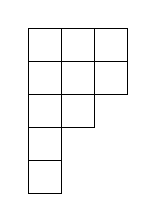
\begin{tikzpicture}[x=4.2mm,y=4.2mm,baseline=(current bounding box.center)]
  \draw (0,0)--(3,0)--(3,-2)--(2,-2)--(2,-3)--(1,-3)--(1,-5)--(0,-5)--cycle;
  \draw (1,0)--(1,-5) (2,0)--(2,-3);
  \draw (0,-1)--(3,-1) (0,-2)--(2,-2) (0,-3)--(1,-3) (0,-4)--(1,-4);
\end{tikzpicture}}\endgroup
\quad \(\begin{gathered}\sum\lambda_j=|\lambda|\\[4pt]\lambda_{i+1}\leqslant\lambda_i\end{gathered}\)}
\end{GelfandAdjacentEvidence}


(\(\lambda_i\) — число клеток в \(i\)-м столбце)

Это соотв. классу сопряж. элементов.


\Needspace{7\baselineskip}
\begin{GelfandAdjacentEvidence}{GELFAND-P001414}{1}
\SourcePage{GELFAND-P001414}{52}

Таблица Юнга:
\[
\begin{aligned}
\text{(6)}\quad t=\{\lambda^{(k)}\}_{k=1}^{N}
&\quad\text{— набор диаграмм, в котором}\\
|\lambda^{(k)}|&=k.
\end{aligned}
\]

Обычное опред. (другое): табл. заполн. числами \(1,2,\ldots,|\lambda|\), причём
\[
\begin{matrix}\rightarrow\\\downarrow\end{matrix}
\quad\text{по этим напр. возрастание}
\]

\SourceFigure{GELFAND-P001414}{tableau-large}{%
\begingroup\color{black}\GelfandFitDiagram{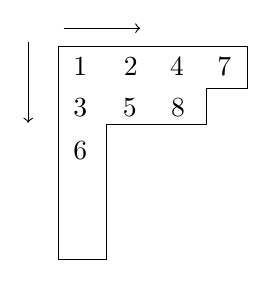
\begin{tikzpicture}[x=6mm,y=6mm]
  \draw (0,0)--(4,0)--(4,-.9)--(3.13,-.9)--(3.13,-1.66)
    --(1,-1.66)--(1,-4.52)--(0,-4.52)--cycle;
  \node at (.45,-.44) {\(1\)};
  \node at (1.52,-.44) {\(2\)};
  \node at (2.50,-.44) {\(4\)};
  \node at (3.50,-.44) {\(7\)};
  \node at (.45,-1.29) {\(3\)};
  \node at (1.50,-1.29) {\(5\)};
  \node at (2.52,-1.29) {\(8\)};
  \node at (.45,-2.22) {\(6\)};
  \draw[->] (.1,.38)--(1.72,.38);
  \draw[->] (-.65,.08)--(-.65,-1.62);
\end{tikzpicture}}\endgroup}
\end{GelfandAdjacentEvidence}
\begin{GelfandAdjacentEvidence}{GELFAND-P001414}{2}


В (6) они должны возрастать

\SourceFigure{GELFAND-P001414}{tableau-growth}{%
\begingroup\color{black}\GelfandFitDiagram{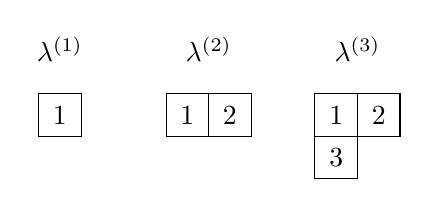
\begin{tikzpicture}[x=5.4mm,y=5.4mm]
  \node at (.5,1.05) {\(\lambda^{(1)}\)};
  \draw (0,0) rectangle (1,-1);
  \node at (.5,-.5) {\(1\)};
  \node at (4,1.05) {\(\lambda^{(2)}\)};
  \draw (3,0) rectangle (5,-1);
  \draw (4,0)--(4,-1);
  \node at (3.5,-.5) {\(1\)};
  \node at (4.5,-.5) {\(2\)};
  \node at (7.5,1.05) {\(\lambda^{(3)}\)};
  \draw (6.5,0)--(8.5,0)--(8.5,-1)--(7.5,-1)--(7.5,-2)--(6.5,-2)--cycle;
  \draw (7.5,0)--(7.5,-1) (6.5,-1)--(7.5,-1);
  \node at (7,-.5) {\(1\)};
  \node at (8,-.5) {\(2\)};
  \node at (7,-1.5) {\(3\)};
\end{tikzpicture}}\endgroup}
\end{GelfandAdjacentEvidence}
\begin{GelfandAdjacentEvidence}{GELFAND-P001414}{3}


\[
\text{(7)}\quad r_k(t)=(i_{k+1}-j_{k+1})-(i_k-j_k)
\]
точка \(k\) имеет координаты \((i_k,j_k)\)

Для диаграммы:
\[
\text{(8)}\quad h(\lambda)=r_\lambda+1
\]
\[
\text{(9)}\quad r_\lambda=\max_{t\in T(\lambda)}\max_{1\leq k\leq N}|r_k(t)|,
\]
где \(T(\lambda)\) — мн-во таблиц, построенных по диаграмме \(\lambda\), т. е. имеющих форму \(\lambda\).
\EvidenceBlock{GELFAND-P001414}{eq9-limit}{В рукописи записано \(1\leq k\leq N\).}{Запись в рукописи.}
\end{GelfandAdjacentEvidence}
\begin{GelfandAdjacentEvidence}{GELFAND-P001414}{4}


Пусть \(s=(\mu^{(k)})_{k=1}^{N}\), \quad \(t=(\lambda^{(k)})_{k=1}^{N}\).

(10) \uline{Опр.}\quad \(s\underset{n}{\approx}t\), если
\(\lambda^{(k)}=\mu^{(k)}\), \(k\ne n\)

\uline{Утверждение.}

(11) [Зачёркнуто: если?] [Вставлено над строкой: Пусть] \(r_n(t)=\pm1\).
Тогда \(s\underset{n}{\approx}t\Rightarrow s=t\).
\Unclear{GELFAND-P001414}{eq11-cancelled-word}{Зачёркнутое слово предположительно читается как «если». Над строкой написано «Пусть».}
\end{GelfandAdjacentEvidence}
\begin{GelfandAdjacentEvidence}{GELFAND-P001414}{5}


(12) Пусть \(|r_n(t)|>1\). Тогда
\(\exists!\ s:\ s\underset{n}{\approx}t,\ s\ne t\).

\[
\text{(13)}\quad S_\lambda^{(k)}=\Vert S_{s,t}^{(k)}(\tau)\Vert_{s,t\in T(\lambda)}
\quad\text{— матрица;}
\]
\Unclear{GELFAND-P001414}{eq13-terminal-mark}{Справа внизу от индекса матрицы виден неразборчивый знак из двух штрихов с загнутым хвостом, возможно \(q\) или исправленная запятая.}
\end{GelfandAdjacentEvidence}
\begin{GelfandAdjacentEvidence}{GELFAND-P001414}{6}


\[
\text{(14)}\quad
S_{s,t}^{(k)}(\tau)=\bigl(W_{r_k(s)}(\tau)\ W_{r_k(t)}(\tau)\bigr)^{1/2}
\quad\text{если }s\underset{k}{\approx}t
\]
\Incomplete{GELFAND-P001414}{eq14-blotted-mark}{После первого множителя виден замазанный знак.}
\end{GelfandAdjacentEvidence}
\begin{GelfandAdjacentEvidence}{GELFAND-P001414}{7}


[Зачёркнуто: если \(s\underset{k}{\approx}t\)\textsuperscript{?}]
и \(S_{s,t}^{(k)}(\tau)=0\) в противном случае.
\Unclear{GELFAND-P001414}{eq14-cancelled-condition}{Зачёркнутое условие предположительно читается как «при \(s\underset{k}{\approx}t\)».}
\end{GelfandAdjacentEvidence}



\Needspace{7\baselineskip}
\begin{GelfandAdjacentEvidence}{GELFAND-P001415}{1}
\SourcePage{GELFAND-P001415}{unlabelled}

(15) \uline{Теорема}. Пусть \(\lambda\) — диагр. из \(N\) элементов и
\(q\ne\sqrt[m]{1}\). Тогда \(S_{\lambda}^{(k)}\) задают представление алгебры Гекке
(в образующих \(e_k\)).
\Unclear{GELFAND-P001415}{theorem-lambda}{В обведённом индексе при \(S^{(k)}\) читается \(\lambda\). Пересекающий штрих сливается с обводкой.}
\end{GelfandAdjacentEvidence}
\begin{GelfandAdjacentEvidence}{GELFAND-P001415}{2}


Построим ф-и \(W\).

\(W_{-r}(\tau)\) при \(r=1,2,\ldots\) опред. из соотношений
\[
\text{(16)}\quad W_{-(r+1)}(\tau)=1-\frac{\tau}{W_{-r}(\tau)},
\qquad r\geqslant0,
\]
[Зачёркнуто: а при \(r\geqslant0\)\textsuperscript{?}]
\Unclear{GELFAND-P001415}{eq16-cancelled}{Два нижних наклонных штриха похожи на соответствующие штрихи знака \(\geqslant\) в (16). Верхний штрих пересекается с зачёркиванием.}
\end{GelfandAdjacentEvidence}
\begin{GelfandAdjacentEvidence}{GELFAND-P001415}{3}

\[
\text{(17)}\quad W_r(\tau)=1-W_{-r}(\tau),\qquad r\geqslant0;
\]

Или:

\(W_{-r}(\tau)\) опр. [Зачёркнуто: неразборчиво] из разл. в цепную дробь:
\Incomplete{GELFAND-P001415}{continued-fraction-cancelled-word}{Слово после «опр.» зачёркнуто и неразборчиво.}
\end{GelfandAdjacentEvidence}
\begin{GelfandAdjacentEvidence}{GELFAND-P001415}{4}


\[
\text{(18)}\quad \text{[Зачёркнуто: }W_{-r}(\tau)=\text{]}\quad
1-\frac{\tau}{1-\dfrac{\tau}{1-\ldots}}
\]
\EvidenceBlock{GELFAND-P001415}{eq18-cancelled-expression}{Перед дробью зачёркнуто \(W_{-r}(\tau)=\).}{Запись в рукописи.}
\end{GelfandAdjacentEvidence}
\begin{GelfandAdjacentEvidence}{GELFAND-P001415}{5}


Имеется ур-е:
\[
\text{(19)}\quad W_r(\tau)W_{1-r}(\tau)=1.
\]
\EvidenceBlock{GELFAND-P001415}{eq19-right-hand-side}{В правой части (19) написано \(1\).}{Запись в рукописи.}
\end{GelfandAdjacentEvidence}
\begin{GelfandAdjacentEvidence}{GELFAND-P001415}{6}


Общая ф-ла:
\[
\text{(20)}\quad W_r(\tau)=\frac{q(q^{r-1}-1)}{(q+1)(q^r-1)},\qquad r=1,2,\ldots
\]
\[
\text{(21)}\quad W_{-r}(\tau)=\frac{q^{r+1}-1}{(q+1)(q^r-1)}.
\]
\EvidenceBlock{GELFAND-P001415}{w-index}{В (20) и (21) у \(W\) и в показателях степени \(q\) написано \(r\).}{Запись в рукописи.}
\end{GelfandAdjacentEvidence}
\begin{GelfandAdjacentEvidence}{GELFAND-P001415}{7}


(22) \uline{Задача}: найти характеры алгебры Гекке.

Рассмотрим
\[
\text{(23)}\quad
\frac{
 \begin{vmatrix}
 x_1^{i_1}&x_1^{i_2+1}&\ldots&x_1^{i_n+n-1}\\
 x_2^{i_1}&x_2^{i_2+1}&\ldots&x_2^{i_n+n-1}\\
 \ldots&\ldots&\ldots&\ldots\\
 x_n^{i_1}&\multicolumn{2}{c}{\ldots}&x_n^{i_n+n-1}
 \end{vmatrix}
}{
 \begin{vmatrix}
 1&x_1&x_1^2&\ldots&x_1^{n-1}\\
 1&x_2&x_2^2&&\\
 &&&&\\
 1&x_n&x_n^2&&x_n^{n-1}
 \end{vmatrix}
}
=\sum a(i,j)P_{j_1}P_{j_2}\ldots P_{j_n}
\]
\Unclear{GELFAND-P001415}{eq23-overwritten-exponents}{В первых двух строках последнего столбца читается \(+n-1\). Индексы при \(i\) переписаны, предположительно \(n\), возможно \(4\). В последней строке индекс \(n\) читается ясно.}
\end{GelfandAdjacentEvidence}



\Needspace{7\baselineskip}
\begin{GelfandAdjacentEvidence}{GELFAND-P001416}{1}
\SourcePage{GELFAND-P001416}{53}

\(j=(j_1,\ldots,j_n)\), \(P_j\) — сумма степеней.

Тогда

(24) \(a(i,j)\) — знач. характера [вставлено над строкой: симм. группы]
на элем. с длинами циклов \(j_1,\ldots,j_n\)

(с точн. до простой константы)

По поводу симм. группы см. книгу Макдональда «Симм. ф-и и многочлены Холла».

\begin{center}
\rule{16mm}{.35pt}\enspace\(\cdot\)\enspace\rule{13mm}{.35pt}
\end{center}

\uline{Локализация полюсов у дзета-функции Рюэлля.}

(Линдон Майер (?))
\EvidenceBlock{GELFAND-P001416}{mayer-name}{В рукописи «Линдон Майер (?)». Вопросительный знак написан автором. Автор цитируемой статьи — Дитер Х. Майер (Dieter H. Mayer), \href{https://doi.org/10.1007/BF00420300}{\emph{On the location of poles of Ruelle’s zeta function}}, Lett. Math. Phys. 14 (1987), 105--115.}{Запись в рукописи.}
\end{GelfandAdjacentEvidence}
\begin{GelfandAdjacentEvidence}{GELFAND-P001416}{2}


Letters in Math. Physics, \(14:2\), 1987 г.

\(I\) — интервал, \(T:I\to I\) — кусочно линейное
\[
 I=\bigcup_j I_j,\qquad T(I_j)=I.
\]

\SourceFigure{GELFAND-P001416}{interval-graph}{%
\begingroup\color{black}\GelfandFitDiagram{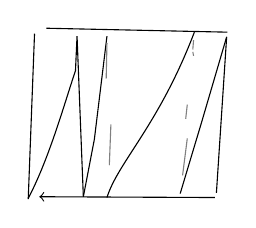
\begin{tikzpicture}[x=10mm,y=10mm]
  \draw (.10,0)--(.18,2.10) (.33,2.17)--(2.63,2.12)
    (2.62,2.06)--(2.49,.08);
  \draw[->] (2.47,.02)--(.24,.03);
  \draw (.10,.01) .. controls (.37,.52) and (.57,1.25) .. (.70,1.63)
    --(.72,2.07)--(.80,.03);
  \draw (.80,.03)--(.94,.76)--(1.10,2.07);
  \draw (1.10,.02) .. controls (1.24,.47) and (1.76,.94) .. (2.21,2.12);
  \draw (2.03,.07)--(2.30,.97)--(2.62,2.06);
  \draw[gray,thin] (1.10,1.98)--(1.09,1.53) (1.15,.95)--(1.13,.43)
    (2.20,2.02)--(2.19,1.90) (2.19,1.87)--(2.20,1.82) (2.12,1.20)--(2.10,1.02) (2.12,.77)--(2.06,.30);
\end{tikzpicture}}\endgroup
\par Принадлежность слабых штрихов ветвям и точное положение разрывов неясны.}
\end{GelfandAdjacentEvidence}
\begin{GelfandAdjacentEvidence}{GELFAND-P001416}{3}


\[
\text{(1)}\quad \zeta_T(z,\varphi)=\frac{\det(1-zL_1)}{\det(1-zL_2)},
\]
где
\[
L_1f(z)=\varphi(z)\sum\frac{1}{\rho_j}f(\psi_j(z)),
\]
\[
L_2f(z)=\varphi(z)\sum f(\psi_j(z)),
\]
\(\psi_j\) — локальные обратные \(T\) на интервале \(I_j\), а \(\rho_j^{-1}\) — наклон.
\Unclear{GELFAND-P001416}{slope-letter}{Буква наклона читается как \(\rho_j\) или \(p_j\).}
\end{GelfandAdjacentEvidence}
\begin{GelfandAdjacentEvidence}{GELFAND-P001416}{4}


В общем случае:
\[
\text{(2)}\quad
\zeta_T(z,\varphi)=\exp\left(
\sum_{n=1}^{\infty}\frac{z^n}{n}
\sum_{\xi\in\mathrm{Fix}\,T^n}
\prod_{k=0}^{n-1}\varphi(T^k x)\right)
\]
\EvidenceBlock{GELFAND-P001416}{eq2-variable}{Под второй суммой написано \(\xi\in\mathrm{Fix}\,T^n\), в произведении — \(x\).}{Запись в рукописи.}
\end{GelfandAdjacentEvidence}


\begin{center}
\rule{16mm}{.35pt}\enspace\(\cdot\)\enspace\rule{16mm}{.35pt}
\end{center}


\Needspace{7\baselineskip}
\begin{GelfandAdjacentEvidence}{GELFAND-P001417}{1}
\SourcePage{GELFAND-P001417}{unlabelled}

\uline{7/XII-87}\qquad \uline{Сем. Гельфанда.}\qquad Нечто о работе

\uline{D. Mayer}\qquad \uwave{Lett. in Math. Phys. 1987, 14:2}

\uline{О \(\zeta\)-функции Рюэлля}

\(F\) — мн-во значений спина (конечное).

Изучаем конфигурации спина на решётке
\[
(\xi_i),\qquad -\infty<i<\infty,\qquad \xi_i\in F.
\]

\(M\subseteq F\times F\) — допустимое мн-во. Требуется, чтобы было
\[
\text{(1)}\quad (\xi_i,\xi_{i+1})\in M
\]

Простейший пример рюэллевской \(\zeta\)-ф-и — \(\zeta\)-ф-я Артина и Мазура.

Рассм. мн-во периодических конфигураций и их количество:
\[
\text{(2)}\quad N_n=\#\{(\xi_i)\mid\mathcal T^n(\xi_i)=(\xi_i)\}
=\mathrm{Fix}\,\mathcal T^n,
\]
\EvidenceBlock{GELFAND-P001417}{eq2-fix}{В конце (2) написано \(\mathrm{Fix}\,\mathcal T^n\) без знака числа элементов.}{Запись в рукописи.}
\end{GelfandAdjacentEvidence}
\begin{GelfandAdjacentEvidence}{GELFAND-P001417}{2}

где \(\mathcal T\) — преобр. в пр-ве послед.
\[
\mathcal T(\xi_i)=\xi_{i+1}
\]
(сдвиг)

\(\zeta\)-ф-я Рюэлля:
\[
\text{(3)}\quad
\zeta_{\mathcal T}(s)=\exp\left(\sum_{n=1}^{\infty}\frac{N_n}{n}s^n\right)
\]
ряд сходится при \(|s|<\dfrac{1}{|F|}\).

Сущ. ли аналитическое продолжение? Рассм. матрицу
\Unclear{GELFAND-P001417}{continuation-question-overwriting}{Конец «Сущ.» и начальная «а» в «аналитическое» обведены поверх прежних штрихов.}
\end{GelfandAdjacentEvidence}

\[
\text{(4)}\quad T=(T_{\alpha\beta})=
\begin{cases}
1,&(\alpha,\beta)\in M,\\
0,&(\alpha,\beta)\notin M.
\end{cases}
\]

Тогда
\[
\text{(5)}\quad\zeta_{\mathcal T}(s)=\frac{1}{\det(1-sT)}
\]

Отсюда видно, что \(\zeta_{\mathcal T}(s)\) мероморфна.

Радиус сход. может быть больше, чем \(1/|F|\).

Для док-ва нужно заметить, что
\[
\text{(6)}\quad N_n=\mathrm{Tr}\,T^n.
\]


\Needspace{7\baselineskip}
\begin{GelfandAdjacentEvidence}{GELFAND-P001418}{1}
\SourcePage{GELFAND-P001418}{62}

\uwave{Замеч. И. М. Г.}: это похоже на раб. Дынкина и Дмитриева:

рассм. стох. матрицу \((p_{ik})\)
[вставлено сверху: (студенческую)] (в задаче о бассейнах это
[зачёркнутый знак: неразборчиво] доля воды, перелив. из \(i\)-го басс. в \(k\)-й).
\EvidenceBlock{GELFAND-P001418}{stochastic-insertion}{Над строкой вставлено «(студенческую)».}{Запись в рукописи.}
\end{GelfandAdjacentEvidence}
\begin{GelfandAdjacentEvidence}{GELFAND-P001418}{2}

\Incomplete{GELFAND-P001418}{basin-cancelled-sign}{Знак перед «доля» зачёркнут и неразборчив.}
\end{GelfandAdjacentEvidence}
\begin{GelfandAdjacentEvidence}{GELFAND-P001418}{3}


\[
\underline{P}=(p_{ik}),\qquad \sum_k p_{ik}=1.
\]

Это зависит от соб. значений \(P\).

а) Соб. значения лежат в круге \(|\lambda|\leq1\),

б) \(1\) — соб. значение.

Какую обл. заполняют соб. значения?

Это внутр. нек-рой алг. кривой.

Они делали неправильно.

Есть набор соб. значений!!

и надо рисовать набор соб. значений в \(\mathbb C^n\) — это должна быть красивая область (\uline{Задача}!!)

Проекция на одну ось может быть сложной!

[Слева двойная черта.]
\uwave{В задаче Рюэлля \uline{интересно} посмотреть все соб. значения матрицы}\quad \(T\).

\smallskip\hrule\smallskip

\uwave{Докладчик.} Обобщение примера (3)
\[
\text{(7)}\quad \zeta_{\mathcal T}(s,\varphi)=
 \exp\left(
 \sum_{n=1}^{\infty}\frac{s^n}{n}
 \sum_{\xi\in\mathrm{Fix}(\mathcal T^n)}
 \prod_{\ell=0}^{n}\varphi(\mathcal T^\ell\xi)
 \right)
\]
\EvidenceBlock{GELFAND-P001418}{eq7-upper-product-bound}{Верхний предел произведения в (7) написан как \(n\).}{Запись в рукописи.}
\end{GelfandAdjacentEvidence}
\begin{GelfandAdjacentEvidence}{GELFAND-P001418}{4}


Здесь
\[
 \underset{\substack{|\\\text{функция}}}{\varphi}
 =\varphi(\xi_1,\ldots,\xi_k),\qquad \xi_j\in F
\]
(\(\varphi\) берётся только от первых \(k\) значений).

((3) получается при \(\varphi=1\))

(8) \uline{Утв.} \(\exists\) [Зачёркнуто: оператор?]
[вставлено сверху: матрица] \(L\) (конечномерная), такая, что:
\Unclear{GELFAND-P001418}{matrix-insertion}{Зачёркнутое слово предположительно читается «оператор». Над ним вписано «матрица».}
\end{GelfandAdjacentEvidence}
\begin{GelfandAdjacentEvidence}{GELFAND-P001418}{5}

\[
\text{(9)}\quad \zeta_{\mathcal T}(s,\varphi)=\frac{1}{\det(1-sL)}
\]

А именно, рассм.
\[
F'=F^k;
\]
[Зачёркнуто: \(F\times F\)\textsuperscript{?}]
\Incomplete{GELFAND-P001418}{before-m-prime-cancelled}{Зачёркнутая запись предположительно читается \(F\times F\). Штриховка скрывает возможные надстрочные знаки.}
\end{GelfandAdjacentEvidence}
\begin{GelfandAdjacentEvidence}{GELFAND-P001418}{6}

\[
M'\subset F'\times F'
\]
\[
\text{(10)}\quad
M'=\{(\xi_1,\ldots,\xi_k);(\xi_2,\ldots,\xi_{k+1})
 \mid(\xi_i,\xi_{i+1})\in M\}
\]
\Unclear{GELFAND-P001418}{eq10-overwritten-indices}{В исправленном втором кортеже читаются индексы \(2\) и \(k+1\), в условии — \(i+1\). Ранние штрихи под обводкой не читаются.}
\end{GelfandAdjacentEvidence}


Тогда надо взять
\[
 \ell_{\alpha\beta}=
 \begin{cases}
 \varphi(\alpha),&(\alpha,\beta)\in M',\\
 0,&(\alpha,\beta)\notin M',
 \end{cases}
 \qquad L=(\ell_{\alpha\beta}).
\]


\Needspace{7\baselineskip}
\begin{GelfandAdjacentEvidence}{GELFAND-P001419}{1}
\SourcePage{GELFAND-P001419}{unlabelled}

\uwave{И. М. Г.}

\uline{NB}: надо знать \(p\)-адич. числа

(уметь их складывать, умножать, делить, [зачёркнуто: неразборчиво] извлекать корни)
\Incomplete{GELFAND-P001419}{nb-cancelled-letter}{Знак после «делить» зачёркнут и неразборчив.}
\end{GelfandAdjacentEvidence}
\begin{GelfandAdjacentEvidence}{GELFAND-P001419}{2}


\uuline{Бейлинсон А.}\qquad \uline{\(p\)-адические числа и физика.}

\uline{О каких-то \(p\)-адических идеях Манина в области физики}!
\Unclear{GELFAND-P001419}{heading-last-sign}{Последний знак похож на «!». Возможно чтение «?».}
\end{GelfandAdjacentEvidence}
\begin{GelfandAdjacentEvidence}{GELFAND-P001419}{3}


\(1^{\circ}\). Виттен слушал доклад Фалтингса с большим интересом, после чего купил все книги по теории чисел.
Единств., что он понял из доклада — это ф-ла
\EvidenceBlock{GELFAND-P001419}{faltings-name}{В рукописи «Фалтингса».}{Запись в рукописи.}
\end{GelfandAdjacentEvidence}
\begin{GelfandAdjacentEvidence}{GELFAND-P001419}{4}

\[
\text{(1)}\quad |a|_\infty\cdot|a|_2|a|_3\ldots=1,\qquad a\in\mathbb Q.
\]

Для \(\dfrac12\) здесь стоит:
\[
\frac12\cdot 2\cdot 1\ldots=1.
\]

Есть 3 статьи:

1) \uwave{Волович}\qquad (по-русски)

2) \uwave{Ю. И. Манин}\qquad (по-английски)

3) \uwave{Witten} и кто-то ещё
\Unclear{GELFAND-P001419}{witten-list-final-sign}{Справа от третьего пункта стоит отдельный неразборчивый знак.}
\end{GelfandAdjacentEvidence}
\begin{GelfandAdjacentEvidence}{GELFAND-P001419}{5}


Все 3 статьи появились в сентябре.

\uwave{Текст Виттена.}

Рассм. функц. ур-е для \(\zeta\)-ф-и Римана
\[
\begin{aligned}
\text{(2)}\quad\pi^{-s/2}\Gamma(s/2)\prod(1-p^{-s})^{-1}
&=\pi^{-(1-s)/2}\Gamma\left(\frac{1-s}{2}\right)
\prod(1-p^{-(1-s)})^{-1}.
\end{aligned}
\]
(аналит. продолжение подразумевается)

или (формально):
\[
\text{(3)}\quad
\frac{\pi^{-s+1}\Gamma(s/2)}{\Gamma\left(\dfrac{1-s}{2}\right)}
=\prod_p\frac{1-p^{-s}}{1-p^{s-1}}.
\]
\EvidenceBlock{GELFAND-P001419}{eq3-pi-exponent}{Показатель степени \(\pi\) написан как \(-s+1\).}{Запись в рукописи.}
\end{GelfandAdjacentEvidence}


Слева \(\approx\) амплитуда Венециано–Виттена для открытой струны [вставлено сверху: (с импульсом \(s\))].
Справа расходящееся выражение, но важно, что она представлена в виде произведения по простым числам!


\Needspace{7\baselineskip}
\begin{GelfandAdjacentEvidence}{GELFAND-P001420}{1}
\SourcePage{GELFAND-P001420}{63}

\uwave{\(2^{\circ}\). О раб. Манина}

(1) \uline{Утверждение}: Мера Тамагавы \(=1\).

Подробнее:
\[
\mathrm{SL}(n,\mathbb R)\supset\mathrm{SL}(n,\mathbb Z).
\]

На \(\mathrm{SL}(n,\mathbb R)\) есть инвар.
[над «инвар.» вставлено: «лево»] мера (стандартная).
\Incomplete{GELFAND-P001420}{measure-tail}{Под концом слова «мера» виден зачёркнутый штрих.}
\end{GelfandAdjacentEvidence}
\begin{GelfandAdjacentEvidence}{GELFAND-P001420}{2}


Нормируем [зачёркнуто: неразборчиво] за счёт целочисл. матриц.
\Incomplete{GELFAND-P001420}{normalization-cancelled}{Запись после «Нормируем» зачёркнута и неразборчива.}
\end{GelfandAdjacentEvidence}
\begin{GelfandAdjacentEvidence}{GELFAND-P001420}{3}

\[
\operatorname{vol}\bigl(\mathrm{SL}(n,\mathbb R)/\mathrm{SL}(n,\mathbb Z)\bigr)-?
\]

[На правом поле:]
(строится по станд. базису в алгебре Ли \(\mathfrak{sl}(n,\mathbb R)\) или в \(\mathfrak{gl}(n,\mathbb R)\)
[зачёркнуто: неразборчиво] станд. базис.
\Incomplete{GELFAND-P001420}{margin-cancelled}{Знак после \(\mathfrak{gl}(n,\mathbb R)\) зачёркнут и неразборчив.}
\end{GelfandAdjacentEvidence}
\begin{GelfandAdjacentEvidence}{GELFAND-P001420}{4}

\[
\boxed{\operatorname{vol}_{sl}=\frac{\operatorname{vol}_{gl}}{d\,\operatorname{tr}}}
\]
\EvidenceBlock{GELFAND-P001420}{margin-volume-formula}{В рамке \(\operatorname{vol}_{sl}=\frac{\operatorname{vol}_{gl}}{d\,\operatorname{tr}}\).}{Запись в рукописи.}
\end{GelfandAdjacentEvidence}
\begin{GelfandAdjacentEvidence}{GELFAND-P001420}{5}


\(\mathrm{SL}(2,\mathbb R)\) — конф. преобр. ед. круга, транзит. действ. на
\(S^*H^2\).

Инвар. объём на \(S^*H^2\) есть [зачёркнуто: неразборчиво]
\(\operatorname{vol}_{H^2}\otimes d\varphi\).
\Incomplete{GELFAND-P001420}{invariant-volume-cancelled}{Знак перед \(\operatorname{vol}_{H^2}\) зачёркнут и неразборчив.}
\end{GelfandAdjacentEvidence}
\begin{GelfandAdjacentEvidence}{GELFAND-P001420}{6}

\EvidenceBlock{GELFAND-P001420}{invariant-volume-letter}{Буква при \(d\) читается как \(\varphi\).}{Запись в рукописи.}
\end{GelfandAdjacentEvidence}
\begin{GelfandAdjacentEvidence}{GELFAND-P001420}{7}


\SourceFigure{GELFAND-P001420}{cotangent-disk}{%
\begingroup\color{black}\GelfandFitDiagram{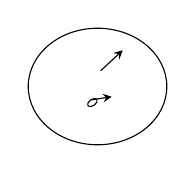
\begin{tikzpicture}[>=stealth,x=10mm,y=10mm]
  \draw (0,0) ellipse[x radius=.88,y radius=.74];
  \draw[rotate=35] (-.17,-.13) ellipse[x radius=.07,y radius=.04];
  \draw[->] (-.08,-.17) -- (.18,-.13);
  \draw[->] (.04,.20) -- (.32,.46);
\end{tikzpicture}}\endgroup}
\end{GelfandAdjacentEvidence}
\begin{GelfandAdjacentEvidence}{GELFAND-P001420}{8}


Или: профакторизовать по max комп. подгруппе

\SourceFigure{GELFAND-P001420}{fundamental-domain}{%
\begingroup\color{black}\GelfandFitDiagram{\begin{tikzpicture}[>=stealth,x=10mm,y=10mm,font=\small]
  \draw (0,0) ellipse[x radius=1.15,y radius=1.04];
  \draw (.02,1.04) .. controls (.06,.61) and (-.03,.23) .. (-.38,-.12);
  \draw (.03,1.04) .. controls (.03,.62) and (.25,.41) .. (.41,.10);
  \draw (-.38,-.12) .. controls (-.13,.14) and (.22,.17) .. (.41,.10);
  \draw (.04,.68)--(.18,.62)
    (-.27,.01) .. controls (-.20,.03) and (-.20,.04) .. (-.18,.12)
    (.31,.12) .. controls (.27,.16) and (.28,.21) .. (.32,.25);
  \node at (.12,.49) {\(0\)};
  \draw (2.65,1.02) .. controls (2.59,.54) and (2.38,.09) .. (1.84,-.30);
  \draw (2.69,1.02) .. controls (2.68,.50) and (3.00,.06) .. (3.32,-.36);
  \draw (1.84,-.30) .. controls (2.34,-.04) and (2.92,-.03) .. (3.32,-.36);
  \draw (2.56,.65)--(2.72,.69)
    (2.12,-.17) .. controls (2.23,-.10) and (2.22,-.01) .. (2.21,.07)
    (3.12,-.24) .. controls (3.04,-.16) and (3.05,-.11) .. (3.09,-.04);
  \node at (2.62,.48) {\(0\)};
  \node at (2.42,.03) {\(\pi/3\)};
  \node at (2.89,.03) {\(\pi/3\)};
  \draw[<-] (3.42,.40)--(3.81,.40);
  \node[anchor=west] at (3.83,.40) {\uwave{фунд. область}};
\end{tikzpicture}}\endgroup}
\end{GelfandAdjacentEvidence}


\uwave{Ответ.}
\[
\text{(2)}\quad
\operatorname{vol}\mathrm{SL}(n,\mathbb R)/\mathrm{SL}(n,\mathbb Z)
=\zeta(2)\zeta(3)\ldots\zeta(n)
\]

\(\mathbb A\) — адели.
\[
\begin{aligned}
\text{(3)}\quad\mathrm{SL}(n,\mathbb A)&\sim
\mathrm{SL}(n,\mathbb R)\times\mathrm{SL}(n,\mathbb Q_2)\times\ldots\\[-2pt]
 &\hspace{3.6em}\begin{gathered}\cup\\\mathrm{SL}(n,\mathbb Q)\end{gathered}
\end{aligned}
\]
\[
\text{(4)}\quad
\operatorname{vol}\mathrm{SL}(n,\mathbb A)/\mathrm{SL}(n,\mathbb Q)=1.
\]
\[
\begin{aligned}
\operatorname{vol}\mathrm{SL}(n,\mathbb A)/\mathrm{SL}(n,\mathbb Q)
 &\sim
 \operatorname{vol}\mathrm{SL}(n,\mathbb R)/\mathrm{SL}(n,\mathbb Z)\\
 &\qquad \prod\operatorname{vol}\mathrm{SL}(n,\mathbb Z_p).
\end{aligned}
\]
\[
\text{(5)}\quad
\operatorname{vol}\mathrm{SL}(n,\mathbb Z_p)
\sim\#\mathrm{SL}_n(\mathbb F_p)/p^{n^2-1}.
\]

\uline{Упражнение}: вычислить \(\#\mathrm{SL}_n(\mathbb F_p)\).


\Needspace{7\baselineskip}
\begin{GelfandAdjacentEvidence}{GELFAND-P001421}{1}
\SourcePage{GELFAND-P001421}{unlabelled}

(6) Число элем. \(\mathrm{GL}(n,\mathbb F_p)\)
\[
\begin{aligned}
 (p^n-1)(p^n-p)(p^n-p^2)\ldots
 &=
 p^{n^2}(1-p^{-n})(1-p^{-n+1})\ldots(1-p^{-1}).
\end{aligned}
\]

(7) Для \(\mathrm{SL}(n,\mathbb F_p)\) надо поделить на \(p-1\):
\[
 p^{n^2-1}(1-p^{-n})(1-p^{-n+1})\ldots(1-p^{-2}).
\]
Это произвед. эйлеровых сомножителей.

(8) \uwave{Гипотеза Ю. И. Манина}: аналог ф-лы (2) можно написать для пр-в модулей кривых, возник. в теории струн.

\uwave{И. М. Г.}

\uwave{Мат. вопрос}: объём пр-ва Тейхмюллера имеет \(p\)-адический аналог.

Или: что такое адельное пр-во Тейхмюллера

\uwave{Пример мощи? работ Виттена:}
\Unclear{GELFAND-P001421}{witten-heading-faint-word}{Бледное слово предположительно читается «мощи». Начальные штрихи сохранились фрагментарно, возможно «силы».}
\end{GelfandAdjacentEvidence}
\begin{GelfandAdjacentEvidence}{GELFAND-P001421}{2}


\uwave{Laumon} сделал раб. по теории чисел на основе идей Виттена из теории Морса.

Идея: рассм. ф-ю \(u\in\mathcal E'(\mathbb R)\),
\(\widetilde u(\xi)\in C^\infty\) и все особ. уйдут в асимптотику на бесконечности.

\uline{Совет И. М. Г.}: прочитать книгу Харкевича «Спектры,
[зачёркнуто: неразборчиво] [вставлено над строкой: сигналы] и шумы»,
чтобы понимать преобр. \uline{Фурье}.
\Incomplete{GELFAND-P001421}{book-title-cancelled}{В названии книги запись зачёркнута. Над ней вписано «сигналы».}
\end{GelfandAdjacentEvidence}
\begin{GelfandAdjacentEvidence}{GELFAND-P001421}{3}


О раб. \uwave{Laumon’а}.

\SourceFigure{GELFAND-P001421}{surface-figure}{%
\begingroup\color{black}\GelfandFitDiagram{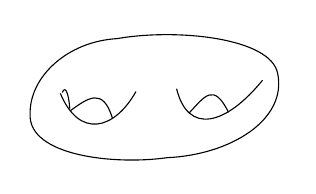
\begin{tikzpicture}[x=12mm,y=12mm]
  \draw (-1.3,-.18) .. controls (-1.31,.21) and (-.91,.59) .. (-.38,.62)
    .. controls (.25,.73) and (1.25,.63) .. (1.32,.25)
    .. controls (1.42,-.24) and (.82,-.61) .. (.15,-.64)
    .. controls (-.41,-.72) and (-1.32,-.62) .. cycle;
  \draw (-.98,.04) .. controls (-.78,-.44) and (-.41,-.35) .. (-.18,.06);
  \draw (-.87,-.14) .. controls (-.69,-.01) and (-.53,.11) .. (-.43,-.22);
  \draw (-.96,.05) .. controls (-.92,.14) and (-.89,.01) .. (-.88,-.12);
  \draw (.25,.09) .. controls (.37,-.40) and (.77,-.30) .. (1.16,.18);
  \draw (.38,-.17) .. controls (.55,.01) and (.64,.16) .. (.80,-.16);
\end{tikzpicture}}\endgroup
\par Короткий штрих у левого края первой петли показан по видимому контуру. Его назначение неясно.}
\end{GelfandAdjacentEvidence}
\begin{GelfandAdjacentEvidence}{GELFAND-P001421}{4}


Рассм. поверхность \(\mathcal F\)
\[
 H^i(X,\mathcal F),\qquad i=0,1,2.
\]
\EvidenceBlock{GELFAND-P001421}{surface-symbol}{После «поверхность» написано \(\mathcal F\), а далее \(H^i(X,\mathcal F)\).}{Запись в рукописи.}
\end{GelfandAdjacentEvidence}
\begin{GelfandAdjacentEvidence}{GELFAND-P001421}{5}


\[
\text{(1)}\quad
\det H^\bullet(X,\mathcal F)=
\frac{\det H^0(X,\mathcal F)\det H^2(X,\mathcal F)}
{\det H^1(X,\mathcal F)\quad\text{[зачёркнуто: }\det H^2(X,\mathcal F)\text{]}}
\]
\Unclear{GELFAND-P001421}{eq1-denominator}{Первый показатель в знаменателе исправлен и читается как \(1\). Зачёркнутый множитель предположительно \(\det H^2(X,\mathcal F)\).}
\end{GelfandAdjacentEvidence}
\begin{GelfandAdjacentEvidence}{GELFAND-P001421}{6}


([зачёркнуто: конечные?] вект. пр-ва.
\(\det\) — макс. внешн. степень)
\Unclear{GELFAND-P001421}{before-vector-spaces-cancelled}{Зачёркнутое слово перед «вект. пр-ва» предположительно читается «конечные».}
\end{GelfandAdjacentEvidence}


Автоморфизмы?

Рассм. триангуляцию. \(\det H^\bullet\) отожд. с произвед. \(\det\)
членов комплекса (ф-ла типа Эйлера): канонически


\Needspace{7\baselineskip}
\begin{GelfandAdjacentEvidence}{GELFAND-P001422}{1}
\SourcePage{GELFAND-P001422}{64}

\[
\text{(2)}\quad\det(C^\bullet)=\det(H^\bullet(C))
\]
\(2-2g\) — эйлерова хар-ка.

С другой стороны
\[
2g-2=\deg\underset{\substack{|\\\text{кан. класс}}}{K}
\]

Пусть

\(D\) — дивизор.
\[
\text{(3)}\quad
\det\mathcal F_D=\bigotimes(\det\mathcal F_{x_i})^{\otimes a_i},
\qquad D=\sum a_i x_i
\]
[зачёркнуто: \(D\longrightarrow D+K\)\textsuperscript{?}]
\Unclear{GELFAND-P001422}{cancelled-divisor-map}{В зачёркнутой записи различимы \(D\), стрелка и предположительно \(D+K\). Начало стрелки пересекают штрихи зачёркивания.}
\end{GelfandAdjacentEvidence}
\begin{GelfandAdjacentEvidence}{GELFAND-P001422}{2}


\uwave{Ф-ла Делиня:}
\[
\text{(4)}\quad\det H^\bullet=\det\mathcal F_K
\]
\EvidenceBlock{GELFAND-P001422}{eq4-determinant-convention}{В (4) справа написано \(\det\mathcal F_K\) без показателя \(-1\).}{Запись в рукописи.}
\end{GelfandAdjacentEvidence}
\begin{GelfandAdjacentEvidence}{GELFAND-P001422}{3}

[Справа: зачёркнуто: неразборчиво]
\Incomplete{GELFAND-P001422}{eq4-cancelled-sign}{Справа от формулы отдельный зачёркнутый знак не читается.}
\end{GelfandAdjacentEvidence}
\begin{GelfandAdjacentEvidence}{GELFAND-P001422}{4}


(фиксир. комплексную структуру и выбор точки в кан. классе)

Для произв. конструкт. пучка тоже считается \(\underline{\det}\) и есть аналог ф-лы Делиня!

Здесь на \(\mathbb A^1\) возникают ф-и с особенностями

\uuline{Клячко.}\qquad \uuline{Торические расслоения.}

Торическое мн-зие — мн-зие \(X\) на к-ром действует алг. тор \(T\),
причём есть орбита, изом. \(T\).
\[
X=\bigcup_\sigma O_\sigma,\quad\text{— разложение на орбиты}
\]

\(\mathcal E\) — расслоение на \(X\) с торической структурой
(и действие поднимается! диагр. коммутативна)

\SourceFigure{GELFAND-P001422}{toric-bundle-square}{%
\begingroup\color{black}\GelfandFitDiagram{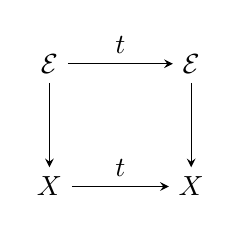
\begin{tikzpicture}[>=stealth,x=12mm,y=12mm]
  \node (source) at (0,1.3) {\(\mathcal E\)};
  \node (target) at (1.5,1.3) {\(\mathcal E\)};
  \node (baseleft) at (0,0) {\(X\)};
  \node (baseright) at (1.5,0) {\(X\)};
  \draw[->] (source) -- node[above]{\(t\)} (target);
  \draw[->] (baseleft) -- node[above]{\(t\)} (baseright);
  \draw[->] (source) -- (baseleft);
  \draw[->] (target) -- (baseright);
\end{tikzpicture}}\endgroup}
\end{GelfandAdjacentEvidence}


Можно описать модули [вставлено над строкой: «таких»] расслоений на языке линейной алгебры.


\Needspace{7\baselineskip}
\begin{GelfandAdjacentEvidence}{GELFAND-P001423}{1}
\SourcePage{GELFAND-P001423}{unlabelled}

Строение \(X\) описывается веером \(\Sigma\) в алгебре Ли тора.

\SourceFigure{GELFAND-P001423}{fan-figure}{%
\begingroup\color{black}\GelfandFitDiagram{\begin{tikzpicture}[>=stealth,x=11mm,y=11mm]
  \draw (-1.49,.89)--(-.06,.02) (-1.39,-.82)--(-.07,-.04);
  \draw (-.19,1.70)--(-.12,.13) (.03,-.07)--(.18,-1.58);
  \draw[->] (0,0)--(.94,1.38);
  \draw[->] (0,0)--(1.80,.92);
  \draw[->] (0,0)--(1.69,-.48);
  \draw (.55,.29)--(.40,.57) (.66,.34)--(.54,.78)
    (.91,.48)--(.73,.95) (1.15,.60)--(.96,1.15) (1.38,.74)--(1.18,1.28);
  \draw (.30,-.09)--(.38,.17) (.52,-.15)--(.61,.29)
    (.80,-.23)--(.91,.41) (1.08,-.31)--(1.20,.51) (1.31,-.28)--(1.42,.62);
  \node at (1.46,1.36) {\(\sigma\)};
  \node at (1.76,.26) {\(\sigma\)};
  \node[anchor=west] at (2.08,.75) {(конусы)};
\end{tikzpicture}}\endgroup}
\end{GelfandAdjacentEvidence}
\begin{GelfandAdjacentEvidence}{GELFAND-P001423}{2}


\(|\Sigma|\) — мн-во \(1\)-мерных конусов в веере \(\Sigma\).

\uline{Теорема.}
(Катег. торич. расслоений) \(\Longleftrightarrow\)
(катег. вект. пр-в [зачёркнут знак: неразборчиво] \(E\)
набором [вставлено над строкой: «убыв. \(\mathbb Z\)-»]
фильтраций \(E^\alpha(i)\), \(\alpha\in|\Sigma|\), удовл. условию
\Incomplete{GELFAND-P001423}{theorem-cancelled-sign}{Зачёркнутый знак перед \(E\) не читается.}
\end{GelfandAdjacentEvidence}
\begin{GelfandAdjacentEvidence}{GELFAND-P001423}{3}


А) Фильтрации \(E^\alpha\), \(\alpha\in\sigma\in\Sigma\), дистрибутивны.

\uline{Задачи.}
1) Описать геометрию расслоения (когом., хар. классы и т. п.) на языке фильтраций

2) классификация — ?

Пусть \(\Sigma\) — симплиц. комплекс. Поставим вершине в соотв. фильтрацию

Его предст. — набор фильтраций в вект. пр-ве [вставлено над строкой: «\(E\):»] \(E^\alpha(i)\),
\(\alpha\in\) [зачёркнут знак: неразборчиво] \(\Sigma\),
\Incomplete{GELFAND-P001423}{representation-cancelled-sign}{Знак между \(\in\) и \(\Sigma\) зачёркнут и неразборчив.}
\end{GelfandAdjacentEvidence}
\begin{GelfandAdjacentEvidence}{GELFAND-P001423}{4}

\[
E\ldots\supset E^\alpha(i)\supset E^\alpha(i+1)\supset\ldots 0
\]
\[
\alpha\in(\text{вершины комплекса})=\Sigma.
\]

Пр-ва \(E^\alpha(i)\), \(\alpha\in\underset{\substack{|\\\text{симплекс}}}{\sigma}\),
дистрибутивны при фиксир. \(\sigma\) (для всех \(i\))

[Вставка в обводке: (т. е. порождают дистрибу. решётку)]

Напр., если

\(\alpha_1,\alpha_2,\alpha_3\) — вершины \(\Delta\)-ка, то

\(E^{\alpha_1}\quad E^{\alpha_2}\quad E^{\alpha_3}\) дистрибутивны, т. е.
\[
(E^{\alpha_1}+E^{\alpha_2})\cap E^{\alpha_3}
=E^{\alpha_1}\cap E^{\alpha_3}+E^{\alpha_2}\cap E^{\alpha_3}
\]

\uwave{Классифицировать}: хорошая задача

Для тр-ка: решается тривиально

Для поверхности тетраэдра \(\Sigma=\partial\Delta\), \(\Delta\) — симплекс, ответ таков: в
[зачёркнуто: \(\mathbb R^3\)-пр-ве?] \(E\), \(\dim E=3\), рассм. \(4\) \(2\)-мерных подпр-ва общего положения.
\Unclear{GELFAND-P001423}{tetrahedron-cancelled-space}{Зачёркнутая запись предположительно читается «\(\mathbb R^3\)-пр-ве». Штрихи зачёркивания пересекают сокращение.}
\end{GelfandAdjacentEvidence}
\begin{GelfandAdjacentEvidence}{GELFAND-P001423}{5}

\[
\mathcal E=(E;\ E^\alpha,E^\beta,E^\gamma,E^\delta)
\]
\Unclear{GELFAND-P001423}{tetrahedron-last-index}{Последний надстрочный знак читается как \(\delta\), как и в следующей записи. Нижняя петля обведена.}
\end{GelfandAdjacentEvidence}



\Needspace{7\baselineskip}
\begin{GelfandAdjacentEvidence}{GELFAND-P001424}{1}
\SourcePage{GELFAND-P001424}{65}
ещё нужно взять [над строкой: их?] внешние степени
\[
\Lambda^i\mathcal E=
(\Lambda^i E,\Lambda^i E^\alpha,\Lambda^i E^\beta,
 \Lambda^i E^\gamma,\Lambda^i E^\delta)
\]
\Unclear{GELFAND-P001424}{exterior-insertion}{Надстрочная вставка предположительно читается «их». Её штрихи пересекаются со знаком вставки.}
\end{GelfandAdjacentEvidence}
\begin{GelfandAdjacentEvidence}{GELFAND-P001424}{2}

Общее предст. разлаг. в прямую сумму \(1\)-мерных и таких.

\uwave{И. М. Г.}
Правильная задача: выделить в \(\forall\) задаче разрешимые куски. (идеология Гельф.—Пономарева)

У В. [зачёркнутый инициал: неразборчиво] \uwave{Каца} всё это описано на языке графов и алгебр
Каца—Муди:
размерности вершин \(=\) коорд. корней и т. п.
\Unclear{GELFAND-P001424}{kac-initial}{Зачёркнутый инициал между «В.» и «Каца» не читается.}
\end{GelfandAdjacentEvidence}
\begin{GelfandAdjacentEvidence}{GELFAND-P001424}{3}


Находится число параметров.

Lect. Notes, \uwave{996}; более ранняя раб. — \uwave{Inventiones}.
(докл. на конференции)

[Зачёркнуто: Семинар? \ldots]
\Unclear{GELFAND-P001424}{cancelled-seminar-line}{Начальное слово зачёркнутой строки предположительно читается «Семинар».}
\end{GelfandAdjacentEvidence}
\begin{GelfandAdjacentEvidence}{GELFAND-P001424}{4}

\Incomplete{GELFAND-P001424}{cancelled-seminar-content}{Остальная часть зачёркнутой строки не читается.}
\end{GelfandAdjacentEvidence}


\uwave{След. раз:}\quad \uwave{8 февраля}.



\clearpage\pdfbookmark[0]{Глава 32}{gelfand-archive-chapter-32}
\section*{Глава 32}


\Needspace{7\baselineskip}
\begin{GelfandAdjacentEvidence}{GELFAND-P001425}{1}
\SourcePage{GELFAND-P001425}{1}
\uline{8/II--88 г.} \quad \uline{Сем. Гельфанда.}

И. М. Г. \uline{Задачи.} 1. Вычислить
\begin{equation*}
\tag{1}\det\left\Vert\frac{1}{x_i-y_k}\right\Vert_{i,k=1}^{n}.
\end{equation*}
2. Док., что полином Лежандра
\[
\bigl((x^2-1)^n\bigr)^{(n)}
\]
имеет только вещественные нули.

3. Может ли ф-я, являющаяся пределом непрерывных функций всюду на отрезке

а) иметь разрывы?

б) иметь всюду плотное м-во точек разрыва?

в) быть всюду разрывной (т. е. в каждой точке)?

4. \textbf{Конформно отобразить на круг}

а) (круг без радиуса!)
\SourceFigure{GELFAND-P001425}{slit-disc}{%
\begingroup\color{black}\GelfandFitDiagram{\begin{tikzpicture}[x=11mm,y=11mm]
  \draw (0,0) circle (.58);
  \draw (0,0)--(.58,0);
  \fill (0,0) circle (.024);
\end{tikzpicture}}\endgroup}
\end{GelfandAdjacentEvidence}
\begin{GelfandAdjacentEvidence}{GELFAND-P001425}{2}


б)
\SourceFigure{GELFAND-P001425}{joined-discs}{%
\begingroup\color{black}\GelfandFitDiagram{\begin{tikzpicture}[>=stealth,x=10mm,y=10mm]
  \draw (.68,.10) arc[start angle=8,end angle=352,radius=.687]
    --(4.82,-.10) arc[start angle=188,end angle=532,radius=.687] --cycle;
  \draw[->] (0,0)--(.19,.65);
  \node[left] at (.10,.35) {\(1\)};
  \draw[->] (5.50,0)--(6.12,.26);
  \node[above] at (5.66,.17) {\(1\)};
  \draw[->] (1.8,.58)--(1.8,.10);
  \draw[->] (1.8,-.62)--(1.8,-.10);
  \node[above right] at (1.8,.26) {\(10^{-6}\)};
  \fill (2.62,0) circle (.022);
  \node[right] at (2.64,-.30) {\(A\)};
  \draw[->] (2.61,-.09)--(2.47,-1.43);
  \draw (2.47,-2.27) circle (.58);
  \draw[->] (2.47,-2.27)--(2.47,-1.69);
  \node[left] at (2.47,-2.04) {\(1\)};
  \node[right] at (2.47,-2.27) {\(0\)};
  \node[anchor=west] at (3.37,-1.36) {\(A\mapsto\) центр круга};
\end{tikzpicture}}\endgroup}
\end{GelfandAdjacentEvidence}
\begin{GelfandAdjacentEvidence}{GELFAND-P001425}{3}


\uuline{\textbf{А. Бейлинсон.}}\qquad \uline{Что нужно знать о теории струн?}

\uline{Конформная теория поля.} \quad (2-мерная)

Операторное разложение.

Связь с представлениями естественных \(\infty\)-мерных алгебр Ли.

\(W\)-алгебры, парафермионы.

[Зачёркнуто: Ве\ldots{} / Вер\ldots{}?] Алгебра \uwave{Вершинных} операторов.
\Unclear{GELFAND-P001425}{vertex-cancellation}{Под зачёркиванием различимо «Ве\ldots{}». Нисходящий штрих может относиться к «р».}
\end{GelfandAdjacentEvidence}
\begin{GelfandAdjacentEvidence}{GELFAND-P001425}{4}

\Unclear{GELFAND-P001425}{vertex-retracing}{Читается «Вершинных». Более ранние штрихи в начале слова неразличимы.}
\end{GelfandAdjacentEvidence}


Различные редукции предст. \(\widehat{SL}_2\) к алгебре Вирасоро.

Связь с пространствами модулей алгебро-геометр. структур.

Явные формулы для стат. сумм и [Зачёркнуто: корреляционных функций; над строкой вставлено: корреляторов].

Свойство ветвления характеров.


\Needspace{7\baselineskip}
\begin{GelfandAdjacentEvidence}{GELFAND-P001426}{1}
\SourcePage{GELFAND-P001426}{unlabelled}
\uuline{Д. Алексеевский.}\qquad \uuline{\(G\)-структуры}

\uwave{Скалярная полевая величина}.

[зачёркнуто: Поле] — функция от точки \(x\in\mathbb R^3\) с векторными значениями

(напр. со знач. в \(\mathbb R\))

\uwave{Полевая величина}: зависит. от сист. координат

\uuline{\(G\)-структура}.

\uuline{Опр. 1}\quad \(G\subset GL(V)\), \(V=\mathbb R^n\).

[Под \(G\): лин. группа.]

\(G\)-структура [над строкой: на \(M^n\)] — главное подрасслоение многообразия всех
[зачёркнуто: ко?]реперов.

[Справа под «реперов»: (кореперов) — лучше говорить.]
\Unclear{GELFAND-P001426}{frame-prefix}{Зачёркнутая запись перед «реперов» предположительно читается «ко». Ниже отдельно написано «(кореперов)».}
\end{GelfandAdjacentEvidence}
\begin{GelfandAdjacentEvidence}{GELFAND-P001426}{2}


\SourceFigure{GELFAND-P001426}{frame-bundle}{%
\begingroup\color{black}\GelfandFitDiagram{\begin{tikzpicture}[>=stealth,x=12mm,y=9mm]
  \node (frames) at (0,0) {\(M^{(1)}\)};
  \node (base) at (2.6,0) {\(M\)};
  \draw[->] (frames) -- node[above] {\(GL(V)\)} (base);
  \node[align=left,anchor=north west] at (-.65,-.26)
    {рассл. реперов \\ (главное расслоение)};
\end{tikzpicture}}\endgroup}
\end{GelfandAdjacentEvidence}
\begin{GelfandAdjacentEvidence}{GELFAND-P001426}{3}


\SourceFigure{GELFAND-P001426}{frame-diagram}{%
\begingroup\color{black}\GelfandFitDiagram{\begin{tikzpicture}[>=stealth,x=11mm,y=9mm]
  \node (frames) at (0,0) {\(M^{(1)}\)};
  \node (base) at (2.7,-.10) {\(M\)};
  \node (reduction) at (0,-1.8) {\(P\)};
  \draw[->] (frames) -- node[above] {\(GL(V)\)} (base);
  \node at (0,-.90) {\(\cup\)};
  \draw[->] (reduction) -- node[below right] {\(G\)} (base);
\end{tikzpicture}}\endgroup}
\end{GelfandAdjacentEvidence}
\begin{GelfandAdjacentEvidence}{GELFAND-P001426}{4}


\(G\) должно действ. на \(P\) транзитивно.
\EvidenceBlock{GELFAND-P001426}{transitivity}{В рукописи написано «на \(P\) транзитивно».}{Запись в рукописи.}
\end{GelfandAdjacentEvidence}
\begin{GelfandAdjacentEvidence}{GELFAND-P001426}{5}


Тогда это и есть \(G\)-структура.

\uline{Примеры}: 1) рим. метрика — это \(O(V)\)-структура

2) Пусть \(S\) — тенз. поле, когда оно задаёт \(G\)-структура?

Если они все одного кан. вида

(в \(\forall\) точке \(\exists\) корепер
[зачёркнуто: \(\theta\) / \(\varphi\)?], прив. \(S\) к фикс. виду)
\Unclear{GELFAND-P001426}{tensor-cancellation}{Зачёркнутый знак после «корепер» похож на \(\theta\) или \(\varphi\).}
\end{GelfandAdjacentEvidence}


Тогда если \(G\) — гр. автоморфизмов кан. вида, то \(S\) зад. \(G\)-структура.

3) Аффинор зад. \(G\)-стр., если в \(\forall\) точке одинак. жорд. форма

4) Почти компл. структура \(J\): \(G=GL\bigl(\frac{n}{2},\mathbb C\bigr)\)

5) Почти симпл. структ.: \(2\)-форма \(\sigma\) макс. ранга,

(\uwave{симпл. стр.}: \(d\sigma=0\))

\uline{Опр. 2}\quad \(G\)-структура — главное \(G\)-расслоение
\(\pi\colon P\overset{G}{\longrightarrow}M\)

\(G\subset GL(V)\)

снабж. векторнозначной \(1\)-формой \(\theta\colon TP\to V\),

облад. след. условиями:


\Needspace{7\baselineskip}
\begin{GelfandAdjacentEvidence}{GELFAND-P001427}{1}
\SourcePage{GELFAND-P001427}{2}
а) \(G\)-эквивариантность

б) \(\operatorname{Ker}\theta=T^vP\) (вертик. пр-во), т. е.
\(\theta\) строго горизонтальна.

\uwave{Эквивалентность определений 1 и 2.}

\(p\in P\), \(x=\pi p\);
\[
\theta_p\colon
\underset{\substack{\downarrow\\ (T_pM/T_p^vM)}}{\underbrace{T_xM}}
\overset{\simeq}{\longrightarrow}V.
\]
[Справа:] это и есть корепер, с к-рым отождествляется точка \(p\).
\EvidenceBlock{GELFAND-P001427}{quotient-notation}{Под \(T_xM\) написано \(T_pM/T_p^vM\), с буквой \(M\) в обоих членах.}{Запись в рукописи.}
\end{GelfandAdjacentEvidence}
\begin{GelfandAdjacentEvidence}{GELFAND-P001427}{2}


[Зачёркнуто: \(\theta_p\) на вертик.? \(\,0\).]
\Unclear{GELFAND-P001427}{zero-cancellation}{Под зачёркиванием различимы \(\theta_p\), «на» и \(0\). Между «на» и \(0\) предположительно написано «вертик\ldots{}».}
\end{GelfandAdjacentEvidence}
\begin{GelfandAdjacentEvidence}{GELFAND-P001427}{3}


Корепер \(\simeq\) изоморфизм
\(\theta_p\colon T_xM\overset{\simeq}{\longrightarrow}V\)

\(\theta\) наз. \uwave{формой смещения}

\begin{center}
\(\rule{1.2cm}{.3pt}\ \cdot\ \rule{1.2cm}{.3pt}\)
\end{center}

Пусть есть \(G\)-структура
\[
(\pi\colon P\overset{G}{\longrightarrow}M;\theta)
\]
Рассм. расслоение 1-струй расслоения \(\pi\)
\[
\pi'\colon P'\to P
\]
\(x\to p_x\) — сечение
\[
p'\colon T_xM\to T_{p_x}P
\]

\uline{Опр.} 1-струя — отобр. \(p'\) — обр. к проекции, \(p'=j_x^1(p)\)

\SourceFigure{GELFAND-P001427}{jet-diagram}{%
\begingroup\color{black}\GelfandFitDiagram{\begin{tikzpicture}[>=stealth,x=10mm,y=8mm]
  \node (label) at (0,0) {\(p'=j_x^1(p)\colon\)};
  \node (base) at (2.16,0) {\(T_xM\)};
  \node (total) at (4.43,0) {\(T_{p_x}P\)};
  \draw[->] (base) -- (total);
  \draw[->] (total.south west) to[bend left=32] (base.south east);
\end{tikzpicture}}\endgroup}
\end{GelfandAdjacentEvidence}
\begin{GelfandAdjacentEvidence}{GELFAND-P001427}{4}

т. е. \(\pi_*\circ p'=\mathrm{id}\)

\uline{Опр.} Горизонтальное подпр-во \(H\subset T_pP\),
[Зачёркнуто: неразборчиво] — такое подпр-во
\Incomplete{GELFAND-P001427}{horizontal-cancellation}{Зачёркнутая запись после \(T_pP\) не читается.}
\end{GelfandAdjacentEvidence}
\begin{GelfandAdjacentEvidence}{GELFAND-P001427}{5}

\[
T_pP=T_p^v\oplus H
\]

\uline{Второе опр. 1-струи}

\[
\underbrace{\text{Элементы }P'}_{\text{(\(=\) 1-струи)}}
=\text{\uwave{горизонт. подпр-ва}}
\]
\[
p'\in P'\quad\Longleftrightarrow\quad H(p')\text{ — горизонт. подпр-во}
\]
\uwave{Связь}:
\[
p'\colon T_xM\to H(p')\subset T_pP
\]
\uline{Опр.} [Зачёркнуто: \(P'\)?]
\(\pi'\) наз. \uwave{расслоением связностей}.
\Unclear{GELFAND-P001427}{connection-cancellation}{Под зачёркиванием перед \(\pi'\) возможно написано \(P'\).}
\end{GelfandAdjacentEvidence}



\Needspace{7\baselineskip}
\begin{GelfandAdjacentEvidence}{GELFAND-P001428}{1}
\SourcePage{GELFAND-P001428}{unlabelled}
\uwave{Пр-во связностей}:\quad \(\Gamma(\pi')^G\)

(т. е. связность — это \(G\)-эквивар. сечение расслоения \(\pi'\colon P'\to P\))

\uwave{Связность}:
\[
\begin{aligned}
h\colon P&\to P'\\
p&\mapsto H(p)
\end{aligned}
\]
(\(G\)-инв. поле горизонт. подпространств)

Отсюда паралл. перенос (огранич. на кривую)

\uline{Функция кручения}\qquad (аналог структ. констант группы Ли)

Есть вертик. параллелизм:
\[
\begin{aligned}
i_p\colon\mathfrak g&\underset{\simeq}{\longrightarrow}T_p^vP\\
X&\mapsto X_p:=\left.\frac{d}{dt}(\exp tX)p\right|_{t=0}
\end{aligned}
\]
\EvidenceBlock{GELFAND-P001428}{vertical-generator}{Точка \(p\) после \((\exp tX)\) обведена. Она написана справа от экспоненты.}{Запись в рукописи.}
\end{GelfandAdjacentEvidence}
\begin{GelfandAdjacentEvidence}{GELFAND-P001428}{2}


\SourceFigure{GELFAND-P001428}{decomposition-diagram}{%
\begingroup\color{black}\GelfandFitDiagram{\begin{tikzpicture}[>=stealth,x=10mm,y=8mm]
  \node at (0,0) {\(p'\in P'\Longrightarrow T_pP=\)};
  \node (vertical) at (3.10,0) {\(T_p^v\)};
  \node at (4.43,0) {\(\oplus H(p')\)};
  \node at (-.62,-.89) {\(\pi'(p')=p\)};
  \node (algebra) at (3.10,-2.12) {\(\mathfrak g\)};
  \draw[->] (vertical) -- node[right] {\(i_p^{-1}\)} (algebra);
\end{tikzpicture}}\endgroup}
\end{GelfandAdjacentEvidence}
\begin{GelfandAdjacentEvidence}{GELFAND-P001428}{3}

[После знака \(=\) зачёркнуто: неразборчиво]
\Incomplete{GELFAND-P001428}{decomposition-cancellation}{Знак между \(=\) и \(T_p^v\) зачёркнут и не читается.}
\end{GelfandAdjacentEvidence}
\begin{GelfandAdjacentEvidence}{GELFAND-P001428}{4}


Возьмём форму \(\theta_p\colon T_pP\to V\)
\Unclear{GELFAND-P001428}{theta-domain}{Оба индекса \(p\) и буква \(P\) обведены или переписаны.}
\end{GelfandAdjacentEvidence}
\begin{GelfandAdjacentEvidence}{GELFAND-P001428}{5}


и положим
\[
\theta_{H(p')}=\theta|_{H(p')}\colon H(p')\overset{\simeq}{\longrightarrow}V
\]
\uline{Опр.}\quad \uwave{ф-я кручения} — это отображение
\[
t\colon P'\longrightarrow\operatorname{Hom}(V\wedge V,V)
\]
(тензоры типа \(1,2\))
\[
p'\mapsto t_{p'},\qquad
t_{p'}(\xi,\eta)=d\theta\bigl(\theta_{H(p')}^{-1}\xi,\theta_{H(p')}^{-1}\eta\bigr)
\]
\EvidenceBlock{GELFAND-P001428}{torsion-last-argument}{Последний знак имеет другую форму начального штриха и читается как \(\eta\).}{Запись в рукописи.}
\end{GelfandAdjacentEvidence}


\uwave{Свойства ф-и кручения}.

1) \(G\)-эквивариантность и \(G'=\operatorname{Hom}(V,\mathfrak g)\)-эквивариантность


\Needspace{7\baselineskip}
\begin{GelfandAdjacentEvidence}{GELFAND-P001429}{1}
\SourcePage{GELFAND-P001429}{3}
\uline{15/II--88 г.}\qquad \uuline{Сем. Гельфанда}
(по записям А. К. Звонкина)

В лекциях И. М. Г. о квазилинейных уравнениях
(\href{https://www.mathnet.ru/eng/rm7290}{УМН-59, т. 14, № 2})
на трёх страницах изложена \uline{вся термодинамика}.

\uwave{Конкр. зад. по геометрии}: что такое угол между двумя \(2\)-мерными подпр-вами в \(4\)-мерном пр-ве?

Угол — инвариант относит. дв-ния (для прямых).

Есть \(2\) варианта: для ориентир. прямых и для неориентированных.

Для плоскостей: сколько этих инвариантов и каковы они?

\uuline{Вопрос}: найти все инварианты двух подпространств гильбертова пространства.

[Зачёркнуто: Зам\ldots{}?]
\Unclear{GELFAND-P001429}{speaker-cancellation}{Зачёркнутая запись над именем предположительно начинается «Зам…».}
\end{GelfandAdjacentEvidence}
\begin{GelfandAdjacentEvidence}{GELFAND-P001429}{2}


\uuline{Замолодчиков Саша.}\qquad
\uline{Конформная (2-мерная) теория поля.}

\begin{equation*}
\tag{1}
\langle A_1(x_1)A_2(x_2)\ldots A_N(x_N)\rangle,\qquad x_i\in\mathbb R^2,
\end{equation*}
— «корреляционные функции»

\(\mathcal A\ni A\) — поля (вообще говоря, \(\infty\)-мерное)

(1) — \(N\)-линейная ф-я на пр-ве полей \(\mathcal A\)
(к тому же ф-я от \((x_1,\ldots,x_N)\))

Уточним понятие среднего в (1):
\begin{equation*}
\tag{2}
(1)=Z^{-1}\int\mathcal D\varphi\, e^{-S[\varphi]}A_1(x_1)\ldots A_N(x_N),
\end{equation*}
где \(\varphi=\varphi(x)\),
\begin{equation*}
\tag{3}
S=\int\sigma\bigl(\varphi(x),\partial\varphi(x)\bigr)\,dx,
\end{equation*}
\begin{equation*}
\tag{4}
Z=\int\mathcal D\varphi\,e^{-S[\varphi]}.
\end{equation*}
\Unclear{GELFAND-P001429}{equation-number}{Номер (4) переписан поверх цифры, похожей на 3.}
\end{GelfandAdjacentEvidence}
\begin{GelfandAdjacentEvidence}{GELFAND-P001429}{3}


\uwave{Свойства корреляционных функций}.

1) «Алгебра полей»

Пусть поля образуют ассоц. алгебру; [Зачёркнуто: неразборчиво]
с [вставлено над строкой: (с континуумом)] [образующими / образующих?] \(A_i(x)\).
\Incomplete{GELFAND-P001429}{algebra-cancellation}{Запись непосредственно после точки с запятой зачёркнута и не читается.}
\end{GelfandAdjacentEvidence}
\begin{GelfandAdjacentEvidence}{GELFAND-P001429}{4}

\Unclear{GELFAND-P001429}{algebra-ending}{Читается основа «образующи». Переписанное окончание допускает чтения «образующими» и «образующих». В \(A_i(x)\) также видны повторные штрихи.}
\end{GelfandAdjacentEvidence}


Пусть \(\{A_i\}\) — базис в \(\mathcal A\). Тогда
\[
A_i(x)A_j(y)=\sum_k
\underset{\substack{\uparrow\\ \text{числовые ф-и от }x,y}}
  {\underbrace{c_{ij}^k(x,y)}}\,A_k(y)
\]

Положим
\[
\langle A_k(x)\rangle=a_k(x)
\]


\Needspace{7\baselineskip}
\begin{GelfandAdjacentEvidence}{GELFAND-P001430}{1}
\SourcePage{GELFAND-P001430}{unlabelled}
(Знания функций \(c_{ij}^k\) и \(a_k\) достаточно для вычисления корреляц. функций:
заменяем пару \(A_1A_2\) на \(\sum c^kA_k\) и т. д.)

2) «\uwave{Инвариантность}»

Рассм. поле \(T\) вида
\[
T^{\mu\nu},\quad\mu,\nu=1,2;\quad T^{\mu\nu}\in\mathcal A.
\]
Кстати
\begin{equation*}
\tag{5}
\frac{\partial}{\partial x^\mu}A_i(x)A_j(y)
=\sum\frac{\partial}{\partial x^\mu}c_{ij}^k(x,y)A_k.
\end{equation*}
\begin{equation*}
\tag{6}
\frac{\partial T^{\mu\nu}}{\partial x^\mu}=0
\end{equation*}

Рассм. [зачёркнуто: оператор?] интеграл
\begin{equation*}
\tag{7}
\oint T^{\mu\nu}(x)A(y)\,\varepsilon_{\mu\lambda}\,dx^\lambda
\end{equation*}
\Unclear{GELFAND-P001430}{integral-cancellation}{Зачёркнутое слово предположительно читается «оператор».}
\end{GelfandAdjacentEvidence}
\begin{GelfandAdjacentEvidence}{GELFAND-P001430}{2}

\Unclear{GELFAND-P001430}{epsilon-first-index}{Второй индекс у \(\varepsilon\) переписан. Читается как \(\lambda\), возможно поверх \(\nu\).}
\end{GelfandAdjacentEvidence}
\begin{GelfandAdjacentEvidence}{GELFAND-P001430}{3}

[Справа от интеграла]
\SourceFigure{GELFAND-P001430}{contour-diagram}{%
\begingroup\color{black}\GelfandFitDiagram{\begin{tikzpicture}[>=stealth]
  \draw (0,0) circle (.56);
  \draw[->] (160:.56) arc[start angle=160,end angle=119,radius=.56];
  \fill (-.05,-.015) circle (.021);
  \node at (.14,-.10) {\(y\)};
\end{tikzpicture}}\endgroup}
\end{GelfandAdjacentEvidence}
\begin{GelfandAdjacentEvidence}{GELFAND-P001430}{4}


[Выносная подпись к \(\varepsilon\) в (7):]
\[
\varepsilon_{\mu\lambda}=-\varepsilon_{\lambda\mu},\qquad\varepsilon_{12}=1
\]
Он определяет линейный оператор в \(\mathcal A\).

\uline{Требуется}: \(\exists\) поле \(T\) такое, что этот оператор равен \(\dfrac{\partial}{\partial y}\).

\(T^{\mu\nu}:=\) «тензор энергии-импульса»
\[
\oint T^{\mu\nu}(x)A_i(y)\,\varepsilon_{\mu\nu}\,dx^\lambda
=\frac{\partial}{\partial y^\nu}A_i(y)
\]
\EvidenceBlock{GELFAND-P001430}{epsilon-repeat}{В повторной формуле второй индекс у \(\varepsilon\) читается как \(\nu\), при \(dx^\lambda\).}{Запись в рукописи.}
\end{GelfandAdjacentEvidence}


\(1')\)\quad \(c_{ij}^k(x,y)=c_{ij}^k(x-y)\) — функции одной переменной в \(\mathbb R^2\).

3) «\uwave{Условие положительности}»

\(A\mapsto A^+\in\mathcal A\) — инволюция
\begin{equation*}
\tag{8}
A_i^+(x)A_j^+(y)=\sum\overline c_{ij}^k(\widetilde x-\widetilde y)A_k^+(y)
\end{equation*}
\[
x=(x^1,x^2)\quad\Rightarrow\quad\widetilde x=(-x^1,x^2)
\]
\uline{Требование}: матрица \(\langle A_i^+(\widetilde x)A_j(x)\rangle\)
положительно определена для всех \(x\).

\uline{Задача} состоит в том, чтобы строить содержательные примеры всего этого.


\Needspace{7\baselineskip}
\begin{GelfandAdjacentEvidence}{GELFAND-P001431}{1}
\SourcePage{GELFAND-P001431}{4}
Введём в \(\mathbb R^2\) комплексные координаты
\[
z=x^1+ix^2\qquad ds^2=dz\,d\bar z
\]
\begin{equation*}
\tag{9}
T^{\nu\mu}=T^{\mu\nu}
\end{equation*}
\begin{equation*}
\tag{10}
\left.\begin{aligned}
T&=T^{zz},\quad \bar T=T^{\bar z\bar z}\\
\Theta&=T^{z\bar z}=0
\end{aligned}\right\}\quad
\begin{gathered}
\text{при этих дополнительных условиях}\\
\text{теория наз.}\\
\text{«конформной теорией поля»}
\end{gathered}
\end{equation*}
[Стрелка снизу к \(\Theta=0\):] Важн. частный случай: безмассовая теория
\EvidenceBlock{GELFAND-P001431}{tensor-components}{В (10) оба верхних индекса при \(\bar T\) имеют черту: \(\bar T=T^{\bar z\bar z}\).}{Запись в рукописи.}
\end{GelfandAdjacentEvidence}
\begin{GelfandAdjacentEvidence}{GELFAND-P001431}{2}


\uline{Контр. вопрос}: записать \(T^{zz}\), \(T^{z\bar z}\), \(T^{\bar z\bar z}\)
через \(T^{\mu\nu}\)

(это задача линейной алгебры)
\begin{equation*}
\tag{11}
\frac{\partial T}{\partial\bar z}=0,\quad
\frac{\partial\bar T}{\partial z}=0
\qquad\text{— уравнения Коши–Римана}
\end{equation*}
\[
\Updownarrow
\]
\(T\) — аналитическая функция \(z\), \(T=T(z)\), \(\bar T=\bar T(\bar z)\).
\begin{equation*}
\tag{12}
T(z)A_i(z_1,\bar z_1)=\sum f_{ij}(z-z_1)A_j(z_1,\bar z_1)
\end{equation*}

\uline{В электродинамике}.

\(\psi\) — электрон

\(A\) — фотон
\[
\{A_i\}=\{\psi,\psi^2,\psi\partial\psi,\ldots,A,A^2,A\psi,\ldots\}
\]
\(\psi^4\) ещё есть, но \(\psi^5=\psi^6=0\) (т. к. всего у спинора 4 компоненты)

у \(A\) есть все степени

Но, вообще говоря, \(A^2\) не существует.

Не надо брать поля в одной точке, надо в разных.
\begin{equation*}
\tag{13}
\oint\frac{dz}{2\pi i}\,z^{n+1}T(z)A_i(z_1,\bar z_1)
=L_nA_i(z_1,\bar z_1)
\end{equation*}
[Справа от (13):]
\SourceFigure{GELFAND-P001431}{mode-contour}{%
\begingroup\color{black}\GelfandFitDiagram{\begin{tikzpicture}
  \draw (0,0) circle (.53);
  \fill (-.08,.035) circle (.021);
  \node at (.14,-.04) {\(z_1\)};
  \node at (0,-.84) {\(n=0,\pm1,\pm2,\ldots\)};
\end{tikzpicture}}\endgroup}
\end{GelfandAdjacentEvidence}

\[
L_{-1}=\frac{\partial}{\partial z_1}
\]
\begin{equation*}
\tag{14}
\bar T(\bar z)\to\bar L_n;\quad
\bar L_{-1}=\frac{\partial}{\partial\bar z_1}
\end{equation*}
\(T(z_1)T(z_2)\) — ф-я от \(z_1\), аналитическая везде, кроме точки \(z_2\);
разложим её в ряд Лорана.


\Needspace{7\baselineskip}
\begin{GelfandAdjacentEvidence}{GELFAND-P001432}{1}
\SourcePage{GELFAND-P001432}{unlabelled}
\begin{equation*}
\tag{15}
T(z_1)T(z_2)=\sum_{m=-\infty}^{\infty}(z_1-z_2)^mT_m(z_2),\qquad
T_m\in\mathcal A
\end{equation*}
Сделаем предположение:
\begin{equation*}
\tag{16}
(15)=(z_1-z_2)^{-4}T_{-4}+(z-z_2)^{-3}T_{-3}+\ldots
\end{equation*}
(т. е. ряд обрывается внизу на члене \(-4\))
\EvidenceBlock{GELFAND-P001432}{laurent-factor}{Второй множитель в (16) записан как \((z-z_2)^{-3}\), без индекса при первом \(z\).}{Запись в рукописи.}
\end{GelfandAdjacentEvidence}
\begin{GelfandAdjacentEvidence}{GELFAND-P001432}{2}

\begin{equation*}
\tag{17}
T_{-1}=\frac{dT}{dz_2}(z_2)
\end{equation*}
\begin{equation*}
\tag{18}
\begin{aligned}
T_{-2}=2T(z_2)&\quad\leftarrow\quad\text{выводится из того, что}\\
&\hphantom{\quad\leftarrow\quad}\text{\(T\) — тензор 2-го ранга}
\end{aligned}
\end{equation*}
Важнее всего определить самые сингулярные слагаемые: \(T_{-3}\) и \(T_{-4}\).

Из условия положительности следует, что
\begin{equation*}
\tag{19}
T_{-4}\sim\text{единичн. оператор}:\quad T_{-4}=\frac c2,\qquad T_{-3}=0
\end{equation*}
\begin{equation*}
\tag{20}
T(z)T(z')=\frac{c}{2(z-z')^4}+\frac{2T(z')}{(z-z')^2}
+\frac{1}{z-z'}T'(z')+\ldots
\end{equation*}
[Стрелка к многоточию в (20):] дальнейшие члены не интересны

Из этого разложения получаем
\begin{equation*}
\tag{21}
\boxed{[L_n,L_m]=(n-m)L_{n+m}+\frac{c}{12}(n^3-n)\delta_{n+m,0}}
\end{equation*}
Это соотн. \uwave{алгебры Вирасоро} (центр. расширение алгебры векторных полей на окружности)

(В обычной квантовой механике — алгебра Ли группы параллельных переносов на прямой: \(\frac{d}{dx}\) — малый перенос — импульс)

Вообще тензор энергии-импульса получается из преобразований координат

В этом смысле квантовую механику придумал Софус Ли: он первый заменил преобразования координат на беск. малые преобразования.

(Для алгебры Вирасоро группой служит группа диффеоморфизмов окружности.)

\end{GelfandAdjacentEvidence}
\begin{GelfandAdjacentEvidence}{GELFAND-P001432}{3}
Длины меньше \(10^{-31}\) см не имеют смысла — это утверждение уже не зависит [зачёркнуто: от / не?]
ни от какой теории — из соотношений между универсальными константами.
\EvidenceBlock{GELFAND-P001432}{length-exponent}{В рукописи показатель читается как \(-31\).}{Запись в рукописи.}
\Unclear{GELFAND-P001432}{lower-cancellation}{Зачёркнутое слово после «зависит» предположительно читается «от», возможно «не».}
\end{GelfandAdjacentEvidence}



\Needspace{7\baselineskip}
\begin{GelfandAdjacentEvidence}{GELFAND-P001433}{1}
\SourcePage{GELFAND-P001433}{5}
\(p\)-адическая теория имеет вычислительные преимущества: некоторые детерминанты лучше всего считать адельным способом

Но есть и ещё одно: физика ничего не может сказать не только о далёких точках, но и о близких.

[Две вертикальные черты слева]
О двумерных многогранниках всё известно, но о трёхмерных и четырёхмерных известно столь же мало, как и 2000 лет назад.

Это новая комбинаторика.
\EvidenceBlock{GELFAND-P001433}{two-dimensional-term}{В рукописи читается «многогранниках». Две черты слева захватывают и строку «Это новая комбинаторика».}{Запись в рукописи.}
\end{GelfandAdjacentEvidence}



Как придумать, что такое пространство, если есть запрет на малые расстояния? Не хватает воображения. (Толщина; дискретность; искривления; \ldots)

\begin{center}
\rule{1.5cm}{.35pt}
\end{center}

Конформная инвариантность: теория не меняется при замене
\begin{equation*}
\tag{22}
\begin{cases}
z\mapsto z+\varepsilon(z)\\
\bar z\mapsto\bar z+\bar\varepsilon(\bar z)
\end{cases}
\end{equation*}
Взяв \(\varepsilon(z)\sim z^{n+1}\), получим алгебру Вирасоро

Выясним, как меняется среднее
\begin{equation*}
\tag{23}
\langle A_1(x_1)\ldots A_N(x_N)\rangle
=Z^{-1}\int A_1(x_1)\ldots A_N(x_N)e^{-S[\varphi]}\,\mathcal D\varphi
\end{equation*}
при заменах
\begin{equation*}
\tag{24}
x^\mu\to x^\mu+\varepsilon^\mu(x)
\end{equation*}
Вариация
\begin{equation*}
\tag{25}
\begin{aligned}
\delta\langle A_1(x_1)\ldots A_N(x_N)\rangle
&=\sum_{k=1}^{N}\langle A_1\ldots\delta_\varepsilon A_k\ldots A_N\rangle\\
&\quad+\int\partial_\mu\varepsilon_\nu
\langle T^{\mu\nu}(x)A_1\ldots A_N\rangle\,d^2x=0
\end{aligned}
\end{equation*}
перебросим (по частям) \(\partial_\mu\) на \(T^{\mu\nu}\) и воспольз.
\(\partial_\mu T^{\mu\nu}=0\);

интегрир. по маленьким контурам, окруж. \(x_1,\ldots,x_N\), получим
\[
\delta_\varepsilon A_k(y)=\oint_{c_y}
\varepsilon_\nu(x)T^{\lambda\nu}(x)\varepsilon_{\lambda\mu}\,dx^\mu A_k(y),
\]
\begin{GelfandAdjacentEvidence}{GELFAND-P001433}{2}
но
\[
\partial_\mu\varepsilon_\nu+\partial_\nu\varepsilon_\mu=\delta_{\mu\nu}g(x);
\]
\Unclear{GELFAND-P001433}{conformal-factor}{Множитель после \(\delta_{\mu\nu}\) предположительно читается \(g(x)\), возможно \(\rho(x)\).}
\end{GelfandAdjacentEvidence}
\begin{GelfandAdjacentEvidence}{GELFAND-P001433}{3}


\(T^{z\bar z}=T^\mu_\mu\) — след; \(=0\).
\EvidenceBlock{GELFAND-P001433}{trace-equality}{В рукописи между \(T^{z\bar z}\) и \(T^\mu_\mu\) написан знак равенства.}{Запись в рукописи.}
\end{GelfandAdjacentEvidence}
\begin{GelfandAdjacentEvidence}{GELFAND-P001433}{4}


[Внизу справа]
\SourceFigure{GELFAND-P001433}{question-figure}{%
\begingroup\color{black}\GelfandFitDiagram{\begin{tikzpicture}[x=10mm,y=10mm]
  \node[align=left,anchor=west] at (0,0) {Что\\получилось};
  \draw (2.90,0) ellipse[x radius=.40,y radius=.48];
  \node at (2.90,0) {?};
\end{tikzpicture}}\endgroup}
\end{GelfandAdjacentEvidence}



\Needspace{7\baselineskip}
\begin{GelfandAdjacentEvidence}{GELFAND-P001434}{1}
\SourcePage{GELFAND-P001434}{unlabelled}
Поля классифицируются по представлениям алгебры Вирасоро.
\begin{equation*}
\tag{26}
\left\{
\begin{aligned}
L_n\phi_\alpha&=0,\quad n>0;&\qquad \bar L_n\phi_\alpha&=0;\\
L_0\phi_\alpha&=\Delta_\alpha\phi_\alpha;&\qquad
\bar L_0\phi_\alpha&=\bar\Delta_\alpha\phi_\alpha;
\end{aligned}
\right.
\end{equation*}
\[
L_{n_N}\ldots L_{n_1}\phi_\alpha=[\phi_\alpha]
\]
\EvidenceBlock{GELFAND-P001434}{descendant-bracket}{Справа от знака равенства в строке потомков написано \([\phi_\alpha]\), с малой \(\phi\).}{Запись в рукописи.}
\end{GelfandAdjacentEvidence}
\begin{GelfandAdjacentEvidence}{GELFAND-P001434}{2}

\[
n_i<0;\quad\Delta_\alpha,\bar\Delta_\alpha\text{ — два числа }\geq0
\]
\[
\mathcal A=\bigoplus_\alpha[\Phi_\alpha]
\]
\[
\mathrm I\in\mathcal A;\qquad\mathrm I\cdot A_i(x)=A_i(x),\qquad
\text{для него }\Delta,\bar\Delta=0
\]
\[
\begin{gathered}
z\to\lambda z\\
\bar z\to\bar\lambda z
\end{gathered}
\qquad \phi_\alpha\to\lambda^{\Delta_\alpha}\bar\lambda^{\bar\Delta_\alpha}\phi_\alpha,
\]
\EvidenceBlock{GELFAND-P001434}{barred-coordinate}{Справа во второй строке написано \(\bar\lambda z\), без черты над \(z\).}{Запись в рукописи.}
\end{GelfandAdjacentEvidence}

\[
\Delta_\alpha-\bar\Delta_\alpha=S_\alpha\text{ — спин }\phi_\alpha.
\]


\Needspace{7\baselineskip}
\begin{GelfandAdjacentEvidence}{GELFAND-P001435}{1}
\SourcePage{GELFAND-P001435}{10}
22.2.8\textsuperscript{?}\quad \uline{Углы между подпространствами}.
\Unclear{GELFAND-P001435}{heading-date}{Последняя цифра даты переписана. Возможны 22.2.88 и 22.2.82. Каталог МЦНМО датирует доклад Гельфанда 22 февраля 1988 г.}
\end{GelfandAdjacentEvidence}


\begin{center}
\uline{Серия задач про углы между подпространствами}

(\uwave{И. М. Гельфанд}; по записям А. К. Звонкина)
\end{center}

Нек-рые доступны 8-класснику (задачи в (\(\mathbb R^2\) и \(\mathbb R^3\)),
другие для доктора наук (задачи в гильб. пр-ве).

Что такое «\uwave{угол}» между двумя прямыми на плоскости?
Это ортогональный инвариант этой пары прямых — т. е. некая числовая хар-ка, к-рая не меняется при всех ортогональных преобр. плоскости.

Более того, угол — это \uwave{полная система инвариантов}, т. е. пара прямых тогда и только тогда переводится в другую пару ортог. пр-ем, когда у этих двух пар прямых одинаковый угол.

В дальнейшем под «углом» понимается полная система инвариантов нек-рого объекта под действием нек-рой группы. Иногда это число, иногда — конечное или счётное мн-во чисел, иногда даже континуум чисел.

(В случаях, когда речь будет идти, скажем, о четвёрке подпр-в \(\Rightarrow\) лин. пр-ва,
не будем употреблять выражение «\dashuline{угол между}\ldots»,
т. к. непонятно, между чем?, а будем говорить «\dashuline{угол для}\ldots».)

Во всех задачах представляет интерес не только то, \dashuline{что такое угол}, но также и \dashuline{какие значения он может принимать}.

\par\noindent I.\quad\uline{Задачи для школьников}.

1. Что такое угол между прямой и плоскостью в трёхмерном пр-ве.

(Два варианта: прямая ориентирована и не ориентирована).

2. Что такое угол между двумя плоскостями в трёхмерном пространстве?

\par\noindent II.\quad\uline{Задачи для студентов}.

3. Дано 4-мерное линейное пр-во со скал. произведением. (не \(\mathbb R^4\), т. к. не выделены оси).
Что такое угол между двумя его двумерными подпространствами?

4. Дано \(\{L,(\cdot,\cdot)\}\), \(\dim L=n\), \(v\in L\),
\(V\subset L\), \(\dim V=k\).

Определить угол между \(v\) и \(V\).


\Needspace{7\baselineskip}
\begin{GelfandAdjacentEvidence}{GELFAND-P001436}{1}
\SourcePage{GELFAND-P001436}{unlabelled}
5. Дано \(\{L,(\cdot,\cdot)\}\), \(\dim L=n\), \(V,W\subset L\),
\(\dim V=k\), \(\dim W=m\). Определить угол между \(V\) и \(W\).
\EvidenceBlock{GELFAND-P001436}{first-v-mark}{У \(V\) в конце задачи 5 видны две раздельные короткие черты, по одной у каждого верхнего конца.}{Запись в рукописи.}
\end{GelfandAdjacentEvidence}


6. Пусть \(L\) — просто линейное пространство (без скалярного произведения). Определить угол для

(а) подпространства \(L\)

(б) пары подпространств

(в) тройки подпространств.

(Под группой здесь надо понимать \(GL(n)\))

7. Дана плоскость Минковского, т. е., \(L\), \(\dim L=2\)
с незнакоопределённым скалярным произведением \(-x_1^2+x_2^2\).
Определить угол между двумя прямыми (т. е. инвариант относительно группы преобразований, сохраняющих это скалярное произведение).

8. Дальнейшие вариации:
\begin{itemize}
\item[—] для пространства Минковского более высокой размерности и двух его подпространств
\item[—] для других пространств с неопределённой метрикой (т. е. когда в скалярном произведении более чем один минус)
\item[—] для пространств с вырожденной формой (\(\mathbb R^3\) со скалярным произведением \(x_1^2+x_2^2\))
\end{itemize}

Для всех перечисленных задач надо рассмотреть случаи групп \(O(n)\) и \(SO(n)\).

\par\noindent III.\quad\uline{Задачи для аспирантов}.

9. Дано лин. пр-во \(L\) и четвёрка его подпр-в.
Найти угол этой четвёрки (это содержание работы Гельфанда и Пономарева)

10. (А. А. Кириллов-младший) Дано \(\{L,(\cdot,\cdot)\}\);
тогда в тензорных степенях \(L\) тоже определено скалярное произведение. Пусть \(a,b\in L\otimes L\).
Найти угол между подпространствами \(a\otimes L\) и \(L\otimes b\),
вложенными в \(L\otimes L\otimes L\).

(Это нужно для алг-р Гекке и ур-я Яна–Бакстера)


\Needspace{7\baselineskip}
\SourcePage{GELFAND-P001437}{11}
\noindent IV.\quad\uline{Задачи для кандидатов и док-торов наук}.

11. Определить угол для двух подпр-в гильбертова пр-ва.

Привести примеры, когда значением угла является счётное мн-во чисел, и когда — континуум чисел.

12. Та же задача для гильбертова пр-ва с неопределённой метрикой.

\uline{Комментарии}.

1. В этих задачах особенно трудна вторая часть; например, если дано подпр-во и угол, а требуется построить другое подпр-во, лежащее под данным углом к данному.

2. Линейный оператор можно задавать с помощью четвёрки подпространств.


\Needspace{7\baselineskip}
\begin{GelfandAdjacentEvidence}{GELFAND-P001438}{1}
\SourcePage{GELFAND-P001438}{unlabelled}
\uline{21/III-88} \qquad \uline{Сем. Гельфанда}

\uuline{Радул А.}

\paragraph*{\uline{Квантовые скобки Гельфанда — Дикого}}
(по С. Лукьянову) \qquad Рассм. на \(S^1\) оператор
\begin{equation*}
L=\partial_z^N+\sum_{i=0}^{N-1}u_{N-1}(z)\partial_z^i . \tag{1}
\end{equation*}
\EvidenceBlock{GELFAND-P001438}{operator-coefficient}{Индекс коэффициента в (1) читается \(N-1\).}{Запись в рукописи.}
\end{GelfandAdjacentEvidence}
\begin{GelfandAdjacentEvidence}{GELFAND-P001438}{2}


и пр-во ф-лов вида
\begin{equation*}
f[u]=\oint P\bigl[z,u_i^{(k)}(z)\bigr]dz \tag{2}
\end{equation*}
и их конечных произведений; \(P\) — полином по \(u_i^{(k)}\).

На таких ф-лах определены 2 скобки Гельфанда — Дикого
\begin{equation*}
\frac{\delta f}{\delta u_i}\qquad
\begin{gathered}\text{опр. из}\\\text{соотн.:}\end{gathered}
\qquad\left.\frac{d}{d\varepsilon}f[u+\varepsilon\delta u]\right|_{\varepsilon=0}
=\oint dz\,\frac{\delta f}{\delta u_i}\delta u_i . \tag{3}
\end{equation*}
\Unclear{GELFAND-P001438}{variation-definition-mark}{Сокращение «опр.» написано поверх повторных штрихов.}
\end{GelfandAdjacentEvidence}
\begin{GelfandAdjacentEvidence}{GELFAND-P001438}{3}


\uwave{И. М. Гельфанд}
\paragraph*{\uline{Отступление о функциональном анализе}}
Вся интуиция функц. анализа исходила из того, что ф-лы — это тоже ф-и, но на \(\infty\)-мерном пр-ве.

И. М. Г. изменил свою точку зрения и отсюда два следствия.

1) Бывают ф-лы разных типов и их надо классифицировать.

2) Ф-лы — не ф-и \(\Rightarrow\) влияет на геометрию.

1) В вар. исчислении бывают ф-лы
\begin{equation*}
\int_0^L f\bigl(x,u(x),u'(x)\bigr)\,dx \tag{*}
\end{equation*}
\EvidenceBlock{GELFAND-P001438}{local-functional-argument}{Аргумент среднего \(u\) читается \(x\).}{Запись в рукописи.}
\end{GelfandAdjacentEvidence}
\begin{GelfandAdjacentEvidence}{GELFAND-P001438}{4}


Это ф-л от \(u\), но он обладает св-вом:

\SourceFigure{GELFAND-P001438}{locality-diagram}{\begingroup\color{black}\GelfandFitDiagram{\begin{tikzpicture}[x=0.8cm,y=0.8cm,baseline=-0.2ex]
\draw (0,0) .. controls (0.36,0.06) and (0.53,0.17) .. (0.76,0.19);
\draw (0.76,0.19) .. controls (0.90,0.21) and (0.83,0.43) .. (0.78,0.55); \draw (0.87,0.24)--(0.96,0.25); \draw (0.99,0.25)--(1.06,0.25);
\draw (0.86,0.68) .. controls (1.00,0.60) and (1.03,0.25) .. (1.16,0.27)
  .. controls (1.67,0.34) and (2.19,0.50) .. (2.65,0.59);
\draw (2.65,0.59) .. controls (2.78,0.61) and (2.75,0.82) .. (2.77,0.96);
\draw (2.83,1.01) .. controls (2.95,1.07) and (3.05,0.84) .. (3.02,0.65)
  .. controls (3.40,0.70) and (3.83,0.87) .. (4.25,0.92); \draw (4.11,0.97) .. controls (4.18,0.97) and (4.23,0.95) .. (4.25,0.92);
\end{tikzpicture}}\endgroup\par Наклонная линия с двумя выступами. В вершинах выступов видны разрывы штрихов. У основания первого выступа есть короткие штрихи. На правом конце линии небольшой крючок.}
\end{GelfandAdjacentEvidence}
\begin{GelfandAdjacentEvidence}{GELFAND-P001438}{5}


если есть приращ. [вставлено над строкой со знаком вставки: \(u\)] в 2-х местах, то приращ. ф-ла (*) будет суммой [зачёркнуто: неразборчиво] приращений
\Unclear{GELFAND-P001438}{locality-cancelled}{Запись после «суммой» зачёркнута. Под штрихами возможна цифра 2 или начало слова «двух».}
\end{GelfandAdjacentEvidence}
\begin{GelfandAdjacentEvidence}{GELFAND-P001438}{6}


(локальность!)

\uwave{5-й [возм.?] обобщ. ф-й:}
\Unclear{GELFAND-P001438}{general-functional-phrase}{Читаются «5-й» и «обобщ.». Сокращение после «5-й» предположительно читается «возм.».}
\end{GelfandAdjacentEvidence}
\begin{GelfandAdjacentEvidence}{GELFAND-P001438}{7}

отсюда вытекает (и из непрерывности), что тогда [зачёркнуто: от / он?] ф-л имеет такой вид
\Unclear{GELFAND-P001438}{general-functional-cancelled}{Зачёркнутая запись после «тогда» предположительно читается «от» или «он».}
\end{GelfandAdjacentEvidence}
\begin{GelfandAdjacentEvidence}{GELFAND-P001438}{8}


[Зачёркнутый знак: неразборчиво.] Это 0-й тип.
\Unclear{GELFAND-P001438}{type-zero-cancelled}{Зачёркнутый знак перед «Это» похож на 1 или И.}
\end{GelfandAdjacentEvidence}



\Needspace{7\baselineskip}
\SourcePage{GELFAND-P001439}{27}
\uwave{1-й тип:} если
\[
\frac{\delta}{\delta u}F(u)\quad\text{\uwave{локален}.}
\]
Таковы ф-лы, встр. в теории Атьи–Зингера

\begin{GelfandAdjacentEvidence}{GELFAND-P001439}{1}
Беда функ. анализа сост. в том, что он [формировался?], когда все [зачёркнуто: это?] пытались рационализировать.
\Unclear{GELFAND-P001439}{analysis-verb}{Видны начало «форм…» и окончание «…вался». Предпочтительное чтение «формировался» остаётся предположительным.}

\Unclear{GELFAND-P001439}{rationalize-cancelled}{Зачёркнутое слово после «все» может читаться «это».}

\EvidenceBlock{GELFAND-P001439}{rationalize-verb}{Глагол перед «рационализировать» читается «пытались».}{Запись в рукописи.}
\end{GelfandAdjacentEvidence}
\begin{GelfandAdjacentEvidence}{GELFAND-P001439}{4}


И [зачёркнуто: спектр?] в теор. ф-й даже непрерывность отн. к обл. смерти.
\Unclear{GELFAND-P001439}{continuity-cancelled}{Зачёркнутый фрагмент после «И» предположительно читается «спектр».}
\end{GelfandAdjacentEvidence}
\begin{GelfandAdjacentEvidence}{GELFAND-P001439}{5}


\paragraph*{\uline{Ф-лы:}}
а) длина кривой

б) площадь поверхности \qquad (локальные)

\paragraph*{\uwave{Трансценд. ф-лы:}}
(как в анализе — невычисляемые интегралы — эллипт. ф-и)

переход от коэфф. к соб. значениям!!

\(\lambda_1\) — такой ф-л

\uwave{Ф-л степ. трансценд. 1} — если вар. производная — лок. ф-л.

и т. д.

\uwave{Ф-л [зачёркнуто: ст. / от?] 2-го типа:} если \(\dfrac{\delta F}{\delta u}\) — 1-го типа.
\Unclear{GELFAND-P001439}{type-two-cancelled}{Зачёркнутое сокращение перед «2-го» похоже на «ст.», возможно «от».}
\end{GelfandAdjacentEvidence}
\begin{GelfandAdjacentEvidence}{GELFAND-P001439}{6}


Продумывали в раб. Гельфанд, Габриэлов, Ло[ши?]к, но заткнулось, т. к. трудно.
\Unclear{GELFAND-P001439}{coauthor-surname}{Фамилия начинается «Ло» и заканчивается «к». Средние соединённые штрихи предположительно читаются «ши». В \href{https://www.mathnet.ru/rus/faa2146}{статье о функционалах Атьи–Патоди–Зингера} третий автор указан как М. В. Лосик.}
\end{GelfandAdjacentEvidence}
\begin{GelfandAdjacentEvidence}{GELFAND-P001439}{7}


В теории [вставлено над строкой: хар.] классов появятся ф-лы всех типов.

Ф-лы надо рассм. на \(\infty\)-мерных мн-зиях. Но не просто заменить \(n\)-мерн. пр-во на \(\infty\)-мерное!

[Зачёркнуто: Род / Тут?] Осн., что локальность играет исключ. роль!
\Unclear{GELFAND-P001439}{locality-cancelled}{Конец зачёркнутой записи перед «Осн.» образует нижнюю петлю. Чтение «Род» или «Тут» предположительно.}
\end{GelfandAdjacentEvidence}


Тогда надо по-другому.

Ф-и образуют алгебру.

Локальные ф-лы не образуют алгебры!!

\uline{Задача:} нужно вариац. исчисление для сумм, произведений таких ф-лов.


\Needspace{7\baselineskip}
\begin{GelfandAdjacentEvidence}{GELFAND-P001440}{1}
\SourcePage{GELFAND-P001440}{unlabelled}
\[
\int f\bigl(x,y;u_i(x),u_i'(x),v_i(y),v_i'(y)\bigr)\,dx\,dy
\]
Поэтому строить дифф. геом. уже нельзя.

Форм. добавить произведения — плохо!

\uwave{Выход;} структуры, введ. \uwave{Г. и Дорфман} и
потом изм. \uline{связность}, \uline{когом. де Рама}, скобки Яна–Бакстера\ldots
\EvidenceBlock{GELFAND-P001440}{structures-word}{Подчёркнутое слово читается «Выход».}{Запись в рукописи.}
\end{GelfandAdjacentEvidence}


\(\underset{\text{(продолжение)}}{\text{\uuline{Радул}}}\)
\qquad Работа: препринт ИПМ; перевод в т. 1 собр. соч.

\paragraph*{Отступление: \uwave{символы п. д. о.}}
\begin{equation*}
A=\sum a_i(z)\partial_z^i,\qquad B=\sum b_j(z)\partial_z^j . \tag{4}
\end{equation*}
\[
\partial_z\longrightarrow\xi
\]
\begin{equation*}
AB=\left.A(z,\xi)\circ B(z,\xi)\right|_{\xi=\partial_z}, \tag{5}
\end{equation*}
где
\[
A(z,\xi)\circ B(z,\xi):=
\sum_{n\geq0}\partial_\xi^n A(z,\xi)\,\partial_z^n B(z,\xi)/n! .
\]

\begin{GelfandAdjacentEvidence}{GELFAND-P001440}{2}
Переключимся на форм. лорановские ряды:
\begin{equation*}
C(z)[[\xi]]=\left\{\sum_{j=-\infty}^{N}c_i(z)\xi^i\right\}. \tag{6}
\end{equation*}
\EvidenceBlock{GELFAND-P001440}{laurent-indices}{В нижнем пределе суммы читается \(j=-\infty\), а в слагаемом \(c_i(z)\xi^i\) два раза написано \(i\).}{Запись в рукописи.}
\end{GelfandAdjacentEvidence}
\begin{GelfandAdjacentEvidence}{GELFAND-P001440}{3}

\Unclear{GELFAND-P001440}{laurent-argument}{В аргументе \(c_i\) видна буква \(z\) поверх прежних штрихов.}
\end{GelfandAdjacentEvidence}
\begin{GelfandAdjacentEvidence}{GELFAND-P001440}{4}


\(\xi^{-1}=\partial_z^{-1}\) обладает [вставлено над строкой: всеми форм.] св-ми опер. интегрирования
\EvidenceBlock{GELFAND-P001440}{formal-insertion}{Над строкой «всеми форм.» со знаком вставки.}{Запись в рукописи.}
\end{GelfandAdjacentEvidence}


Операции на символах
\begin{equation*}
\left(\sum_{-\infty}^{N}a_i\xi^i\right)_+=\sum_0^N a_i\xi^i \tag{7}
\end{equation*}
\begin{equation*}
\operatorname{res}\left(\sum_{-\infty}^{N}a_i\xi^i\right)=a_{-1} \tag{8}
\end{equation*}

\uline{Градиент \(f\).}
\begin{equation*}
\nabla f:=\sum_{j=0}^{N-1}\xi^{-j-1}\circ\frac{\delta f}{\delta u_j}. \tag{9}
\end{equation*}


\Needspace{7\baselineskip}
\begin{GelfandAdjacentEvidence}{GELFAND-P001441}{1}
\SourcePage{GELFAND-P001441}{28}
Тогда
\begin{equation*}
\delta f=\oint\operatorname{res}\delta L\circ\nabla f \tag{10}
\end{equation*}
здесь \(L\) — оператор (1)

1-я скобка (гам. структура)
\begin{equation*}
1\text{ ГС:}\quad \{f,g\}_1:=\oint\operatorname{res}[L,\nabla f]\nabla g \tag{11}
\end{equation*}
2-я скобка:
\begin{equation*}
2\text{ ГС:}\quad \{f,g\}_2=
\oint\operatorname{res}\bigl(L(\nabla f L)_+-(L\nabla f)_+L\bigr)\nabla g \tag{12}
\end{equation*}

(13) \uline{Утв.} \(\{\,\}_i\) [зачёркнуто: неразборчиво] задаёт на пр-ве ф-лов структуру алгебры Ли.
\Incomplete{GELFAND-P001441}{statement-cancelled}{Запись между \(\{\,\}_i\) и «задаёт» зачёркнута и не читается.}
\end{GelfandAdjacentEvidence}
\begin{GelfandAdjacentEvidence}{GELFAND-P001441}{2}

\Unclear{GELFAND-P001441}{statement-verb}{Видно начало «зада…». Конец переписан, глагол предположительно читается «задаёт».}
\end{GelfandAdjacentEvidence}
\begin{GelfandAdjacentEvidence}{GELFAND-P001441}{3}


(14) \uline{Пример.} \(N=2\), \(u_1=0\), \(\partial_z^2+u_2\).

Пусть
\begin{equation*}
u_2(n)=\frac12\,\frac{1}{2\pi i}\oint u_2(z)z^{n+1}\,dz \tag{15}
\end{equation*}
Тогда
\begin{equation*}
\{u_2(n),u_2(m)\}_2=\frac{n^3-n}{12}\delta_{n+m,0}+(n-m)u_2(n+m) \tag{16}
\end{equation*}
(получ. коммут. соотн. алг. Вирасоро!)

(17) \uline{Пример.} \(N=3\), \(u_1=0\), \(\partial_z^3+u_2\partial_z+u_3\).
\Unclear{GELFAND-P001441}{example-number}{В номере (17) вторая цифра переписана и читается как 7.}
\end{GelfandAdjacentEvidence}
\begin{GelfandAdjacentEvidence}{GELFAND-P001441}{4}

\begin{equation*}
\{u_2(n),u_2(m)\}_2=\frac{n^3-n}{6}\delta_{n+m,0}+(n-m)u_2(n+m)
\tag*{$(18)_{\text{а}}$}
\end{equation*}
\begin{equation*}
\{u_2(n),u_3(m)\}_2=3(n+1)u_3(m+n)-(m+n+3)u_3(m+n)
\tag*{$(18)_{\text{б}}$}
\end{equation*}
\Unclear{GELFAND-P001441}{mixed-bracket-letter}{В (18)б у первого \(u_2(n)\) утолщены штрихи \(u\), а индекс читается 2.}
\end{GelfandAdjacentEvidence}
\begin{GelfandAdjacentEvidence}{GELFAND-P001441}{5}

\begin{equation*}
\{u_3(n),u_3(m)\}_2=\ldots+
\sum_{k=-\infty}^{\infty}(m+n-k)u_2(m+n-k)u_2(k)
\tag*{$(18)_{\text{в}}$}
\end{equation*}
(квадрат тензора энергии-импульса)

Далее всюду \(\{\,\}\) означает \(\{\,\}_2\).

Вместе это классич. предел какой-то квантовой алг. токов.
\EvidenceBlock{GELFAND-P001441}{final-abbreviation}{Перед «токов» написано «алг.».}{Запись в рукописи.}
\end{GelfandAdjacentEvidence}



\Needspace{7\baselineskip}
\begin{GelfandAdjacentEvidence}{GELFAND-P001442}{1}
\SourcePage{GELFAND-P001442}{unlabelled}
\uwave{Мораль.} получается не классич. алгебра Ли, а алгебра с квадр. соотношениями.

(Хованова Т.)

Дынкин тоже вводил квадр. соотн.

С. Лукьянов заним. квантованием этих скобок.

[Слева под именем: (Серёжа)]
(С. Лукьянов — асп. В. Фатеева)

\paragraph*{\uline{Отступление}}
\uwave{Преобразование Миуры.} Пусть
\begin{equation*}
L(z)=\partial_z^N+\sum u_{N-i}\partial_z^i
=(\partial_z+v_1)\ldots(\partial_z+v_N) \tag{19}
\end{equation*}
\EvidenceBlock{GELFAND-P001442}{miura-index}{В (19) индекс у \(u\) читается \(N-i\), с точкой над \(i\).}{Запись в рукописи.}
\end{GelfandAdjacentEvidence}
\begin{GelfandAdjacentEvidence}{GELFAND-P001442}{2}

\begin{center}— \(\cdot\) —\end{center}
\(\underset{\text{\uline{И. М. Г.}}}{\text{\uline{замеч.}}}\)\qquad
Если \((\partial_z+v_1)(\partial_z+v_2)u=f\), то \(u\) нах. в квадратурах.

Алг. ур-е в радикалах — теория Галуа

Для дифф. ур-й соотв. теория — теория Пикара–Вессио.

Сейчас этим занимается [зачёркнуто: Кол…?] Колчин.
\Unclear{GELFAND-P001442}{kolchin-cancelled}{Зачёркнутая запись перед «Колчин» предположительно начинается «Кол…».}
\end{GelfandAdjacentEvidence}
\begin{GelfandAdjacentEvidence}{GELFAND-P001442}{3}


\begin{center}— \(\cdot\) —\end{center}
\uuline{Р.}

\uwave{Разлож.} (19): Миура\\
\hspace*{3em}Купершмидт — Вильсон\\
\hspace*{3em}Дринфельд — Соколов

(20) \uline{Теорема.} Зададим для \(v_j\) коммут. соотношения
\begin{equation*}
\{v_i(n),v_j(m)\}=h\delta_{ij}\,n\delta_{m+n,0} . \tag{21}
\end{equation*}
[Справа: (алг. Ли — алг. [перечёркнутый знак] Гейзенберга)]
\EvidenceBlock{GELFAND-P001442}{heisenberg-factor}{Множитель перед \(\delta_{ij}\) читается \(h\).}{Запись в рукописи.}
\end{GelfandAdjacentEvidence}
\begin{GelfandAdjacentEvidence}{GELFAND-P001442}{4}

\Unclear{GELFAND-P001442}{heisenberg-sign}{Перед «Гейзенберга» перечёркнутый знак, похожий на \(H\) или \#.}
\end{GelfandAdjacentEvidence}
\begin{GelfandAdjacentEvidence}{GELFAND-P001442}{5}


Тогда \(u_i\) удовлетворяют алгебр. Г.-Д. соотнош. (Гельф.-Дикого)

(2-я структура Г.-Д., здесь и ниже)

Получилось, что алг. Ли изоморфна [зачёркнуто: квад…?] квадр. алгебре, не являющейся алгеброй Ли.
\Unclear{GELFAND-P001442}{quadratic-cancelled}{Зачёркнутая запись перед «квадр.» предположительно начинается «ква…» или «квад…».}
\end{GelfandAdjacentEvidence}


Пусть теперь
\begin{equation*}
L(z)={:}(\partial_z+v_1)\ldots(\partial_z+v_N){:} \tag{22}
\end{equation*}
Какие соотношения?

Введём


\Needspace{7\baselineskip}
\begin{GelfandAdjacentEvidence}{GELFAND-P001443}{1}
\SourcePage{GELFAND-P001443}{29}
\[
M_0=\operatorname{Hol}\bigl((\mathbb C\backslash0)_z\times
(\mathbb C\backslash0)_w\longrightarrow\mathbb C\bigr)
\]
[Под \(\operatorname{Hol}\): гол. отобр.]
\[
M=\operatorname{Hol}\bigl(((\mathbb C\backslash0)_z\times
(\mathbb C\backslash0)_w\backslash\Delta)\longrightarrow U(v_1,\ldots,v_N)\bigr)
\]
[К \(U\) проведена черта от пояснения: универ. оберт. алгебра алгебры Гейзенберга.]

Элемент \(M\) — операторнозначная ф-я.

Рассм. ещё оператор
\[
\tau=\frac{\nu}{2}\ln(z-w)^2\,\sigma,\qquad \sigma f(z,w)=f(w,z).
\]
на ф-ях 2-х переменных
\Unclear{GELFAND-P001443}{operator-letter}{Знак с верхней перекладиной предположительно читается \(\tau\), возможно \(r\). Он повторяется в (23).}
\end{GelfandAdjacentEvidence}
\begin{GelfandAdjacentEvidence}{GELFAND-P001443}{2}


Тогда если \(\nu(\nu-1)=h\), то
\begin{equation*}
\exp(-\tau)L(z)L(w)\exp\tau\,[f]=\underline{\underline{O}}(1)
\quad\text{при }z\longrightarrow w \tag{23}
\end{equation*}
\[
\forall f\in M_0
\]
\Unclear{GELFAND-P001443}{boundedness-symbol}{Знак перед \((1)\) обведён и дважды подчёркнут. Предположительно читается \(O\), возможно \(0\).}
\end{GelfandAdjacentEvidence}
\begin{GelfandAdjacentEvidence}{GELFAND-P001443}{3}


Это набор соотношений на \(u_i\) (на коэффициенты)

Результат:
\begin{equation*}
[u_i(z),u_j(w)]=
\left[\sum_{k\geq2}(z-w)^{-k}
\sum_{p+q=i+j-k}c_{ij}^{pq}(k)[u_p(z),u_q(w)]\right] \tag{24}
\end{equation*}
[Под правой внешней скобкой стрелка \(\uparrow\) от подписи «\(+\) или \(-\)».]
\Unclear{GELFAND-P001443}{sum-lower-limit}{Под первой суммой предположительно написано \(k\geq2\). Знак между \(k\) и 2 не вполне ясен и может читаться как \(=\).}

\EvidenceBlock{GELFAND-P001443}{bracket-arrow}{Стрелка от подписи «\(+\) или \(-\)» направлена к правой внешней скобке (24).}{Запись в рукописи.}
\end{GelfandAdjacentEvidence}
\begin{GelfandAdjacentEvidence}{GELFAND-P001443}{5}


\(c_{ij}^{pq}(k)\) выраж. через гипергеометрич. ф-и, но сложно

Форма [под словом: ск[…].] (23) похожа на соотн. в квант. методе обр. задачи.
\Unclear{GELFAND-P001443}{formula-subline}{В начале сокращения предположительно читается «ск…». Средние штрихи бледны, их пересекает нижний штрих буквы верхнего слова. В конце видна точка.}
\end{GelfandAdjacentEvidence}

\begin{equation*}
L(z)L(w)=R^{-1}L(w)L(z)R. \tag{25}
\end{equation*}


\Needspace{7\baselineskip}
\begin{GelfandAdjacentEvidence}{GELFAND-P001444}{1}
\SourcePage{GELFAND-P001444}{unlabelled}
\paragraph*{\uuline{М. Капранов.}}
\uline{Представления колчанов и производная категория.}

(\uline{О раб. Партасарати о предст. колчанов.})
\EvidenceBlock{GELFAND-P001444}{reference-name}{Фамилия читается «Партасарати». Ср. статью \href{https://repository.ias.ac.in/82619/1/1-Pub.pdf}{Р. Партасарати о \(t\)-структурах в производной категории представлений колчанов}.}{Запись в рукописи.}
\end{GelfandAdjacentEvidence}
\begin{GelfandAdjacentEvidence}{GELFAND-P001444}{2}


\uwave{Колчан} — ориент. граф без циклов
\SourceFigure{GELFAND-P001444}{definition-quiver}{\begingroup\color{black}\GelfandFitDiagram{\begin{tikzpicture}[x=0.65cm,y=0.65cm,>=stealth]
\coordinate (left) at (0,0);
\coordinate (top) at (1.4,0.9);
\coordinate (right) at (2.1,-0.03);
\coordinate (bottom) at (0.9,-1.0);
\draw[->] (left) -- (top);
\draw[->] (top) -- ([yshift=2pt]right);
\draw[->] (left) -- (right);
\draw[->] (left) -- (bottom);
\draw[->] (bottom) -- ([yshift=-2pt]right);
\end{tikzpicture}}\endgroup}
\end{GelfandAdjacentEvidence}
\begin{GelfandAdjacentEvidence}{GELFAND-P001444}{3}


\(\Lambda\) — граф

\(\Omega\) — ориентация

\(M(\Lambda,\Omega)\) — [зачёркнуто: пр…?] категория представлений колчана
\Unclear{GELFAND-P001444}{category-cancelled}{Зачёркнутая запись перед «категория» предположительно начинается «пр…», возможно «кат…».}
\end{GelfandAdjacentEvidence}
\begin{GelfandAdjacentEvidence}{GELFAND-P001444}{4}


\(\mathcal D(\Lambda,\Omega)\) — производная категория этой категории.

(1) \uline{Лемма.}

Тогда \(\mathcal D(\Lambda,\Omega)\) не зависит от \(\Omega\)

(\(\mathcal D(\Lambda,\Omega_1)\) и \(\mathcal D(\Lambda,\Omega_2)\) эквивалентны)

при разных \(\Omega_1\) и \(\Omega_2\)

\uline{Д-во:} применение симметрии.

\uline{Задача:} найти такие
[зачёркнуто: \(\mathcal D^{\ell}(\mathcal A)\)?] подкатегории \(\mathcal A\subset\mathcal D(\Lambda,\Omega)\), что
\[
\mathcal D^{\ell}(\mathcal A)=\mathcal D(\Lambda,\Omega)
\]
\Unclear{GELFAND-P001444}{derived-cancelled}{Зачёркнутая формула предположительно читается \(\mathcal D^{\ell}(\mathcal A)\). Верхний знак похож также на \(e\).}
\end{GelfandAdjacentEvidence}
\begin{GelfandAdjacentEvidence}{GELFAND-P001444}{5}

\Unclear{GELFAND-P001444}{subcategory-sign}{Знак \(\subset\) обведён. Внутри различим угловой штрих.}
\end{GelfandAdjacentEvidence}
\begin{GelfandAdjacentEvidence}{GELFAND-P001444}{6}

\Unclear{GELFAND-P001444}{derived-exponent}{Над \(\mathcal D\) в рукописи стоит знак, похожий на \(\ell\) или \(e\). В статье Партасарати для ограниченной производной категории используется \(\mathcal D^b\).}
\end{GelfandAdjacentEvidence}
\begin{GelfandAdjacentEvidence}{GELFAND-P001444}{7}


Все они найдены и характериз. графами Дынкина.

Используются отражения и склейки (и идеология извращённых пучков)

\uline{Замеч. И. М. Г.} Классифик. вект. рассл. на \(CP^n\) делается только на языке производных категорий.

\uline{Гротендик:} тяжёлым трудом добыл понятия, ведущие к производной категории (как Микеланджело).

\uuline{М. К.}

\SourceFigure{GELFAND-P001444}{reflection-quiver}{\begingroup\color{black}\GelfandFitDiagram{\begin{tikzpicture}[x=0.70cm,y=0.70cm,>=stealth]
\coordinate (left) at (0,0);
\coordinate (top) at (2.1,1.25);
\coordinate (right) at (4.4,0.15);
\coordinate (bottom) at (1.15,-1.55);
\node[left] at (left) {\(V_\alpha\)};
\node[above right] at (top) {\(V_\beta\)};
\node[right] at (right) {\(V_\gamma\)};
\draw[->] (left) -- node[above left] {\(f\)} (top);
\draw[->] (top) -- ([yshift=2pt]right);
\draw[->] (left) -- node[above] {\(\scriptstyle[?]\)} (right);
\draw[->] (left) -- (bottom);
\draw[->] (bottom) -- ([yshift=-2pt]right);
\end{tikzpicture}}\endgroup\par Над средней стрелкой перечёркнутый знак, возможно \(g\) или \(\varphi\). Нижняя вершина без подписи.}
\end{GelfandAdjacentEvidence}
\begin{GelfandAdjacentEvidence}{GELFAND-P001444}{8}


\uwave{Отражение} а) \(s_\alpha\Omega\) — обращаем стрелки, исходящие из \(\alpha\).

б)
\[
(s_\alpha V)_{\beta\ne\alpha}=V_\beta
\]
\[
(s_\alpha V)_\alpha=\bigoplus_{\alpha\to\beta}V_\beta/(\text{образу }V_\alpha)
\]
с естеств. отображениями

Могут быть векторы из \(V_\alpha\), к-рые всюду переходят в \(0\)

\SourceFigure{GELFAND-P001444}{zero-kernel-quiver}{\begingroup\color{black}\GelfandFitDiagram{\begin{tikzpicture}[x=0.72cm,y=0.62cm]
\coordinate (left) at (0,0);
\node[above left] at (left) {\(V_0\)};
\draw (left) -- (2.0,0.9) node[right] {\(V_1\)};
\draw (left) -- (1.5,-0.7) node[right] {\(V_2\)};
\draw (left) -- (0.9,-1.85) node[right] {\(V_3\)};
\end{tikzpicture}}\endgroup}
\end{GelfandAdjacentEvidence}


\[
V_0\longrightarrow V_1\oplus V_2\oplus V_3
\]


\Needspace{7\baselineskip}
\begin{GelfandAdjacentEvidence}{GELFAND-P001445}{1}
\SourcePage{GELFAND-P001445}{30}
Построим комплекс по этим данным

\SourceFigure{GELFAND-P001445}{derived-object-diagram}{\begingroup\color{black}\GelfandFitDiagram{\begin{tikzpicture}[x=0.65cm,y=0.72cm,>=stealth]
\node (complex) at (0.0,0) {\(\{V_0\longrightarrow V_1\oplus V_2\oplus V_3\}\)};
\node (v1) at (0.15,-1) {\(V_1\)};
\node (v2) at (0.08,-2) {\(V_2\)};
\node (v3) at (0,-3) {\(V_3\)};
\node at (3.25,0) {\(0\)};
\node at (3.25,-1) {\(1\)};
\node at (3.25,-2) {\(2\)};
\node at (3.25,-3) {\(3\)};
\draw[->] (v1.north west) to[out=145,in=250] (0.10,-0.24);
\draw[->] (v2.west) to[out=160,in=245] (-0.18,-0.24);
\draw[->] (v3.west) to[out=170,in=241] (-0.46,-0.24);
\end{tikzpicture}}\endgroup}
\end{GelfandAdjacentEvidence}
\begin{GelfandAdjacentEvidence}{GELFAND-P001445}{2}


Это объект производной категории (предст. колчана)

\SourceFigure{GELFAND-P001445}{reflected-star-diagram}{\begingroup\color{black}\GelfandFitDiagram{\begin{tikzpicture}[x=0.67cm,y=0.67cm,>=stealth]
\node (zero) at (0,0) {\(0\)};
\node (one) at (2.25,0.93) {\(1\)};
\node (two) at (2.3,-0.30) {\(2\)};
\node (three) at (1.4,-1.95) {\(3\)};
\draw[->] (one) -- (zero.15);
\draw[->] (two) to[out=182,in=-20] (zero.-20);
\draw[->] (three) to[out=115,in=-52] (zero.-52);
\end{tikzpicture}}\endgroup}
\end{GelfandAdjacentEvidence}
\begin{GelfandAdjacentEvidence}{GELFAND-P001445}{3}


Факторизации в обычной кат. надо сопоставлять само отображение (комплекс)

Партисарати ставит и решает вопрос о том, когда производная катег. совп. с этой (для \(3^{\text{\uline{х}}}\), но не для \(4^{\text{\uline{х}}}\)).
\EvidenceBlock{GELFAND-P001445}{bottom-name}{На этом кадре написано «Партисарати».}{Запись в рукописи.}
\end{GelfandAdjacentEvidence}



\Needspace{7\baselineskip}
\begin{GelfandAdjacentEvidence}{GELFAND-P001446}{1}
\SourcePage{GELFAND-P001446}{unlabelled}
\uline{23. III. 88 г.}\qquad\uline{Сем. Гельфанда.}

\uuline{Зелевинский А.}\qquad\uline{Матроиды и теорема Холла}

\uline{И. М. Г.}

Матроид. [Над следующим словом зачёркнуто: неразборчиво.] \uline{Пример:} линейно независ. системы векторов.
\Incomplete{GELFAND-P001446}{intro-deletion}{Запись над «Пример» зачёркнута и не читается.}
\end{GelfandAdjacentEvidence}
\begin{GelfandAdjacentEvidence}{GELFAND-P001446}{2}

\[
M_1,M_2\text{ — мн-ва},\qquad \varphi\subset M_1\times M_2
\]
\hfill (отношение)\par

Пусть на \(M_1\) есть структ. \uwave{матроида}.

Как ввести структ. матроида на \(M_2\)?
\[
A\subset M_2,\qquad
\pi_1\bigl(\pi_2^{-1}(A)\cap\varphi\bigr)\text{ — мн-во}.
\]
\Incomplete{GELFAND-P001446}{image-set-deletion}{Под тире перед «мн-во» запись зачёркнута и не читается.}
\end{GelfandAdjacentEvidence}
\begin{GelfandAdjacentEvidence}{GELFAND-P001446}{3}


Ранг мн-ва \(A\) определяется

\(1^\circ\). \uline{Теор. Радо}
\[
r_{M_2}(A)=\min_{B\subset A}
\bigl(r_{M_1}(\varphi(B))+|A-B|\bigr),\qquad A\subset M_2.
\]
\EvidenceBlock{GELFAND-P001446}{rank-retrace}{В формуле ранга знак \(\varphi\) в \(\varphi(B)\) обведён.}{Запись в рукописи.}
\end{GelfandAdjacentEvidence}
\begin{GelfandAdjacentEvidence}{GELFAND-P001446}{4}


\(2^\circ\). \uline{Теор. Холла} \(\equiv\) [Над фамилией вставлено: Ф.?]
\Unclear{GELFAND-P001446}{hall-insertion}{У знака, вставленного перед «Холла», есть вертикальная черта и разомкнутая петля. Возможно, это «Ф.»; назначение знака неясно.}
\end{GelfandAdjacentEvidence}
\begin{GelfandAdjacentEvidence}{GELFAND-P001446}{5}


[Зачёркнуто слева: неразборчиво.] \uline{Зад. о выборе невест.}
\Incomplete{GELFAND-P001446}{hall-left-deletion}{Запись слева от «Зад.» зачёркнута и не читается.}
\end{GelfandAdjacentEvidence}
\begin{GelfandAdjacentEvidence}{GELFAND-P001446}{6}


Если [над \(N\) вписано: мн-во] \(N\) невест и [зачёркнуто: \(M\geq N\) женихов] [вставлено сверху: мн-во \(M\) женихов, \(\operatorname{Card}M\geq\operatorname{Card}N\)], каждому жениху \(m\in M\) нравятся невесты \(A(m)\subset N\);
\EvidenceBlock{GELFAND-P001446}{grooms-insertion}{Над зачёркнутым «\(M\geq N\) женихов» стоит вставка с записью \(\operatorname{Card}M\geq\operatorname{Card}N\).}{Запись в рукописи.}
\end{GelfandAdjacentEvidence}
\begin{GelfandAdjacentEvidence}{GELFAND-P001446}{7}


причём [зачёркнуто: \(\forall A\subset N\)] \(\forall\) подмн-ва \(K\subset N\),
\[
\operatorname{Card}\left(\bigcup_{n\in K}B(n)\right)
\geq \operatorname{Card}K.
\]
\Incomplete{GELFAND-P001446}{card-deletion}{Знак над \(\operatorname{Card}\) зачёркнут и не читается.}
\end{GelfandAdjacentEvidence}
\begin{GelfandAdjacentEvidence}{GELFAND-P001446}{8}

\EvidenceBlock{GELFAND-P001446}{bride-neighbour}{В последней формуле обведена буква \(B\) в \(B(n)\).}{Запись в рукописи.}
\end{GelfandAdjacentEvidence}



\Needspace{7\baselineskip}
\begin{GelfandAdjacentEvidence}{GELFAND-P001447}{1}
\SourcePage{GELFAND-P001447}{37}
(Здесь \(B(n)\subset M\);
[Под \(B(n)\) через знак равенства:] мн-во женихов, к-рым нравится \(n\), т. е.
\[
B(n)=\{m:\ n\in A(m)\}
\]
[После \(=\) зачёркнуто: неразборчиво.])
\Incomplete{GELFAND-P001447}{top-b-deletion}{Знак между \(=\) и открывающей скобкой зачёркнут и не читается.}
\end{GelfandAdjacentEvidence}
\begin{GelfandAdjacentEvidence}{GELFAND-P001447}{2}


Тогда \(\exists\) вз.-однозн. выбор [зачёркнуто: неразборчиво]: отображение
\[
f\colon N\longrightarrow M,
\]
для к-рого
\[
f(n)\subset B(n)\qquad \forall n.
\]
\Incomplete{GELFAND-P001447}{choice-deletion}{Запись после «выбор» зачёркнута и не читается.}
\end{GelfandAdjacentEvidence}
\begin{GelfandAdjacentEvidence}{GELFAND-P001447}{3}

\EvidenceBlock{GELFAND-P001447}{hall-membership}{Между \(f(n)\) и \(B(n)\) в рукописи стоит знак \(\subset\).}{Запись в рукописи.}
\end{GelfandAdjacentEvidence}
\begin{GelfandAdjacentEvidence}{GELFAND-P001447}{4}


[Зачёркнута строка: Теор. Холла \(\quad\varphi\) — отношение.]

[Зачёркнуто: Теор.] Сущ. док-во, содержащее алгоритм.

\uline{Сведение к теор. Радо:} в \(N\) надо объявить все мн-ва независимыми.
\EvidenceBlock{GELFAND-P001447}{rado-letter}{Буква после «в» написана густо и читается \(N\).}{Запись в рукописи.}
\end{GelfandAdjacentEvidence}
\begin{GelfandAdjacentEvidence}{GELFAND-P001447}{5}


\(2^\circ\Rightarrow3^\circ\). \uline{Теор. Биркгофа.}

Из теор. Холла следует, что если есть подгруппа \(H\subset G\)
[Под \(G\): кон. группа], то \(\exists\) \uwave{система общих представителей} левых и правых смежных классов.

\uline{И. М. Г.} Есть \uwave{неск. знаменитых задач, про к-рые всем очевидна их бессмысленность.}

\uline{Пример.} 1) \uline{Аксиома о параллельности}

(почему именно она?)

[Под строкой:] занимались [многие?]
\Unclear{GELFAND-P001447}{parallelism-note}{Под вопросом написано «занимались». Следующее слово предположительно читается «многие».}
\end{GelfandAdjacentEvidence}
\begin{GelfandAdjacentEvidence}{GELFAND-P001447}{6}


[Справа от первых двух строк, за вертикальной чертой:] \(\Rightarrow\) неевкл. геом.

2) Трисекция угла и квадратура круга.
\SourceFigure{GELFAND-P001447}{trisection-arrow}{\begingroup\color{black}\GelfandFitDiagram{\begin{tikzpicture}[x=1cm,y=0.52cm]
\node (top) at (0,0) {\uline{Трисекция угла}};
\node at (0,-1) {\(\Downarrow\)};
\node at (0,-2) {теор. Галуа};
\end{tikzpicture}}\endgroup}
\end{GelfandAdjacentEvidence}
\begin{GelfandAdjacentEvidence}{GELFAND-P001447}{7}


3) Теор. Ферма
\SourceFigure{GELFAND-P001447}{fermat-arrow}{\begingroup\color{black}\GelfandFitDiagram{\begin{tikzpicture}[x=1cm,y=0.48cm]
\node at (0,0) {\uline{Теор. Ферма}};
\node at (0,-1) {\(\Downarrow\)};
\node[align=center] at (0,-2.3) {теор. [зачёркнуто: неразборчиво] идеалов (Куммер)\\и алгебр. геометрия.};
\end{tikzpicture}}\endgroup}
\end{GelfandAdjacentEvidence}
\begin{GelfandAdjacentEvidence}{GELFAND-P001447}{8}

\Incomplete{GELFAND-P001447}{ideals-deletion}{Перед «идеалов» стоит неразборчивый зачёркнутый знак.}
\end{GelfandAdjacentEvidence}
\begin{GelfandAdjacentEvidence}{GELFAND-P001447}{9}

[Справа, за вертикальной чертой:] раб. Фалтингса.

4) Задача о \(4^{\text{х}}\) красках
\SourceFigure{GELFAND-P001447}{four-colour-arrow}{\begingroup\color{black}\GelfandFitDiagram{\begin{tikzpicture}[x=1cm,y=0.50cm]
\node at (0,0) {\uwave{Задача о \(4^{\text{х}}\) красках}};
\node at (0,-1) {\(\Downarrow\)};
\node at (0,-2) {?};
\end{tikzpicture}}\endgroup}
\end{GelfandAdjacentEvidence}


Стоит разобрать эти работы.

5) \uline{Гипотеза Римана}


\Needspace{7\baselineskip}
\begin{GelfandAdjacentEvidence}{GELFAND-P001448}{1}
\SourcePage{GELFAND-P001448}{unlabelled}
\uline{А. Рудаков.}\quad
\uline{Векторные расслоения, группы кос и диофантовы уравнения.}

\(1^{\circ}\). На \(\mathbb{P}^{2}\ (= \mathbb{C}\mathbb{P}^{2})\)

рассм. вект. расслоения (или ког. пучки)
\EvidenceBlock{GELFAND-P001448}{sheaf-retrace}{В слове «пучки» последние буквы обведены густо.}{Запись в рукописи.}
\end{GelfandAdjacentEvidence}
\begin{GelfandAdjacentEvidence}{GELFAND-P001448}{2}

\begin{equation*}
E_1,\ E_2,\ E_3 \tag{1}
\end{equation*}
\Incomplete{GELFAND-P001448}{triple-deletion}{После \(E_1\) зачёркнуты неразборчивые знаки.}
\end{GelfandAdjacentEvidence}
\begin{GelfandAdjacentEvidence}{GELFAND-P001448}{3}

\begin{equation*}
\begin{gathered}
\operatorname{Ext}^{k}(E_j,E_i)=0,\quad j>i,\quad k=0,1,2,\\
\operatorname{Ext}^{k}(E_i,E_i)=
\begin{cases}
0,& k>0,\\
\mathbb{C},& k=0.
\end{cases}
\end{gathered}
\tag{2}
\end{equation*}
\Incomplete{GELFAND-P001448}{ext-deletion}{Перед \(k=0,1,2\) зачёркнут неразборчивый знак.}
\end{GelfandAdjacentEvidence}
\begin{GelfandAdjacentEvidence}{GELFAND-P001448}{4}


Такие существуют и если \(\dim E_j=x_j\), то
\begin{equation*}
x_1^2+x_2^2+x_3^2=3x_1x_2x_3
\qquad\text{(ур-е Маркова)} \tag{3}
\end{equation*}
(и все [сверху вставлено: целочисл.] решения так реализуются!)

На наборах [сверху вставлено: (1) (их счётное мн-во)] действ. \uline{группа кос} и все наборы (1) сост. 1 орбиту!

\(2^{\circ}\).
\begin{equation*}
Q=\mathbb{P}^{1}\times\mathbb{P}^{1}.
\end{equation*}
\Incomplete{GELFAND-P001448}{quadric-deletion}{После \(Q=\) зачёркнут неразборчивый знак.}
\end{GelfandAdjacentEvidence}
\begin{GelfandAdjacentEvidence}{GELFAND-P001448}{5}


Тогда берём 4 расслоения \(E_1,E_2,E_3,E_4\) с теми же условиями (2); тоже действ. группа кос.

Вместо (3) возникает система диофантовых ур-й
(но соответствие в одну сторону; не доказано, что все реш. получаются).
Это что-то вроде системы корней, где вместо гр. Вейля возникает группа кос.

\(3^{\circ}\). На \(\mathbb{P}^{n}\) можно рассм. расслоения
\begin{equation*}
E_1,E_2,\ldots,E_{n+1}\qquad\text{с усл. (2)}
\end{equation*}
и тоже возникает действие группы кос.

\uline{М. Капранов}: о действии группы кос.

\uline{И.М.Г.}

Разрешимые и неразрешимые классификационные задачи.

Нет парам. \(\Rightarrow\) классифицируются (ручные)

1 парам \(\Rightarrow\)
[зачёркнуто: «[ручные?]» и неразборчивая запись в скобках; над строкой вставлено: полуручные] (tame)
\Unclear{GELFAND-P001448}{classification-correction}{Над зачёркнутой строкой читается «полуручные», справа «(tame)». Первое зачёркнутое слово похоже на «ручные»; запись в скобках не читается.}
\end{GelfandAdjacentEvidence}
\begin{GelfandAdjacentEvidence}{GELFAND-P001448}{6}


\(\geq 2\) парам. \(\Rightarrow\) неразреш. (напр., пары матриц)

и классиф. отн.
\Incomplete{GELFAND-P001448}{bottom-deletion}{Перед отображением зачёркнута неразборчивая запись.}
\end{GelfandAdjacentEvidence}

\begin{equation*}
(A,B)\mapsto(C^{-1}AC,C^{-1}BC).
\end{equation*}


\Needspace{7\baselineskip}
\begin{GelfandAdjacentEvidence}{GELFAND-P001449}{1}
\SourcePage{GELFAND-P001449}{38}
В неразреш. задачах всегда есть разрешимая часть
(открытая орбита!)

\Unclear{GELFAND-P001449}{top-deletion}{Над инициалами зачёркнут знак. Он похож на «Еф»; возможно, это начало \(\operatorname{Ext}\).}
\end{GelfandAdjacentEvidence}
\begin{GelfandAdjacentEvidence}{GELFAND-P001449}{2}

\uline{М.К.}
\[
\operatorname{Ext}^{1}(E,E)=0\ \Rightarrow\ \text{жёсткость}
\]
(и рассл. такие не имеют параметров)

\Unclear{GELFAND-P001449}{sequence-deletion}{Над началом последовательности зачёркнуто короткое слово. Возможно, «Пару».}
\end{GelfandAdjacentEvidence}
\begin{GelfandAdjacentEvidence}{GELFAND-P001449}{3}

\[
0\longrightarrow R\longrightarrow E\otimes\operatorname{Hom}(E,F)
\longrightarrow F
\]

Пару \((E,F)\) назовём исключительной, если \(\operatorname{Ext}^{j}(F,E)=0\).

Тогда пара \((F,R)\) тоже исключительна.
\EvidenceBlock{GELFAND-P001449}{pair-order}{В рукописи стоит именно \((F,R)\).}{Запись в рукописи.}
\end{GelfandAdjacentEvidence}
\begin{GelfandAdjacentEvidence}{GELFAND-P001449}{4}


Получ. действие \(\mathbb{Z}\) на таких парах; выполняются соотношения, дающие косы.

И.М.Г. \uline{Работа} Берншт.-Гельф.-Пономарев:

в предст. графов действ. гр. Кокстера.

\uwave{Что нужно для занятий, напр., спектр. теорией из общего образ.}

1) Предст. графов (4-ка подпр-в и т.п.)

2) Произв. категория.

\uuline{Бейлинсон А.}\qquad \uline{Извращенные пучки.}

И.М.Г.

(о Макферсоне)
\SourceFigure{GELFAND-P001449}{circle-diagram}{\begingroup\color{black}\GelfandFitDiagram{\begin{tikzpicture}[x=.021cm,y=-.021cm,line cap=round,line join=round]
\coordinate (A) at (107,21);
\coordinate (T) at (177,12);
\coordinate (U) at (238,43);
\coordinate (B) at (252,145);
\coordinate (V) at (251,158);
\coordinate (D) at (181,205);
\coordinate (C) at (66,193);
\coordinate (L) at (27,97);
\draw (A) .. controls (149,3) and (203,6) .. (U)
  .. controls (269,65) and (276,110) .. (B)
  .. controls (241,172) and (214,192) .. (D)
  .. controls (147,217) and (103,217) .. (C)
  .. controls (19,174) and (5,140) .. (13,96)
  .. controls (23,52) and (57,27) .. (A);
\draw (A) .. controls (138,74) and (182,119) .. (250,145)
  -- (258,151);
\draw (A) .. controls (140,66) and (124,124) .. (C)
  .. controls (112,156) and (205,144) .. (V) -- (258,161);
\draw (A) .. controls (103,72) and (69,88) .. (L)
  .. controls (68,113) and (85,147) .. (C);
\draw (19,97) -- (L);
\draw (A) .. controls (142,57) and (153,46) .. (T)
  .. controls (196,41) and (208,52) .. (U);
\draw[thin] (A) .. controls (142,65) and (207,66) .. (U);
\draw (U) .. controls (213,74) and (230,121) .. (B);
\draw (228,67) .. controls (239,82) and (251,81) .. (260,83)
  .. controls (241,89) and (243,111) .. (255,124);
\draw (C) .. controls (106,172) and (153,166) .. (D)
  .. controls (201,173) and (222,164) .. (V);
\end{tikzpicture}}\endgroup\par{\footnotesize В правом нижнем узле штрихи перекрываются; точное соединение линий неясно.}}
\end{GelfandAdjacentEvidence}
\begin{GelfandAdjacentEvidence}{GELFAND-P001449}{5}


Чем параметризовать эти области?
\SourceFigure{GELFAND-P001449}{projective-line-rows}{\begingroup\color{black}\GelfandFitDiagram{\begin{tikzpicture}[x=.78cm,y=.74cm,line cap=round]
\draw (0,0) -- (2.7,.13);
\foreach \x/\y in {.65/.03,1.24/.015,1.84/.04,2.46/.11}
  \draw (\x,\y) circle[radius=1.35pt];
\draw (0,-.9) -- (2.65,-.78);
\foreach \x/\y in {.65/-.88,1.24/-.85,1.84/-.82}
  \draw (\x,\y) circle[radius=1.35pt];
\draw[thin] (3.06,.07) -- (3.06,-.3);
\node[anchor=west,align=left,text width=3.7cm,font=\footnotesize] at (3.2,.11) {4 точки на проект. прямой};
\node[anchor=west,font=\footnotesize] at (3.2,-.83) {стираем};
\end{tikzpicture}}\endgroup}
\end{GelfandAdjacentEvidence}
\begin{GelfandAdjacentEvidence}{GELFAND-P001449}{6}

Обл. Зигеля \(\Rightarrow\) конфигур. прямых на \(\mathbb{R}\mathbb{P}^{2}\).

\uuline{Б.}

О раб. \uwave{Макферсона} (о его раб. с \uline{Гельфандом} и Виллоненом(?))
\Unclear{GELFAND-P001449}{vilonen-reading}{Фамилия предположительно читается «Виллоненом», с двумя «л». Вопросительный знак в скобках есть в рукописи.}
\end{GelfandAdjacentEvidence}


Извращ. пучки?

Извр. пучку соотв. задачи лин. алгебры, его полностью описывающие, но неясно, как выделить извращ. пучки.


\Needspace{7\baselineskip}
\begin{GelfandAdjacentEvidence}{GELFAND-P001450}{1}
\SourcePage{GELFAND-P001450}{unlabelled}
\(X\) — компл. мн-ие (гладкое)

Конструктивный пучок.

Задана стратификация \(\{X_i\}\) [над \(X_i\) с отводной чертой: откр.],
пучок \(\mathcal F\) на \(X\) наз. конструкт.
[вписано снизу: отн. неё],
если \(\mathcal{F}|_{X_i}\) — локально пост. пучок конечномерных вкт. пр-в.

(локально — отн. обычной топ.)

Конструктивные комплексы пучков
\begin{equation*}
\ldots\longrightarrow\mathcal{F}^{-1}
\longrightarrow\mathcal{F}^{0}
\longrightarrow\mathcal{F}^{1}
\longrightarrow\mathcal{F}^{2}\longrightarrow\ldots \tag{1}
\end{equation*}
комплекс пучков наз. конструктивным, если все пучки \(H^{i}(\mathcal{F}^{\bullet})\) конструктивны.

(на \(\mathcal{F}^{i}\) условий нет!)

\uwave{Синг. носитель} пучка или комплекса.

\(\mathcal{F}^{\bullet}\) — констр. комплекс.
\begin{equation*}
SS(\mathcal F)\subset T^*X \tag{2}
\end{equation*}
[Под \(SS(\mathcal F)\): подмн-ие]

определяется след. образом.

Пусть \(\nu\in T_x^{*}X,\ \nu\ne0\).
\Unclear{GELFAND-P001450}{covector-letter}{Знак ковектора читается как \(\nu\) или латинское \(v\).}
\end{GelfandAdjacentEvidence}
\begin{GelfandAdjacentEvidence}{GELFAND-P001450}{2}


(3) \uline{Опр.}
\[
\nu\notin SS(\mathcal{F})\ \Longleftrightarrow
\]
[Сверху вставлено: если] выб. малую окр. \(U\ni x\), голом. ф-ю \(f\) на \(U\),
для к-рой \(df_x=\nu\), \(f(x)=0\), то \(\forall\) близкой к \(0\) точки \(\varepsilon\in\mathbb C\)
\begin{equation*}
H^{*}\bigl(U,\underset{\cap\,U}{f^{-1}(\varepsilon)};\mathcal{F}\bigr)=0. \tag{4}
\end{equation*}
(относит. гр. когом. mod слоя)

(точнее, надо перех. к индукт. пределу)

([зачёркнуто: [появл.?]] \(\ne0\ \Longleftrightarrow\) появл. исчез. циклов)
\Unclear{GELFAND-P001450}{cycles-deletion}{Зачёркнутая запись предположительно читается «появл.».}
\end{GelfandAdjacentEvidence}


(4) от выбора \(f\) не зависит

0-е сечение?

Добавляем 0-е сечение, если \(\mathcal F^{\bullet}\) — ненулевой комплекс.

\(\mathcal F^{\bullet}\) — нулевой
\(\Rightarrow SS(\mathcal F^{\bullet})\overset{\mathrm{def}}{=}\varnothing\).


\Needspace{7\baselineskip}
\begin{GelfandAdjacentEvidence}{GELFAND-P001451}{1}
\SourcePage{GELFAND-P001451}{39}
(5) \uline{Теорема.}
\(SS(\mathcal{F})\) — коническое лагранжево подмн-ие

(аналитич. подмн-ие, у к-рого неособые точки лагранжевы в обычном смысле [зачёркнут знак]; равносильное условие — инволют. идеала)
\Unclear{GELFAND-P001451}{sense-correction}{Зачёркнутый знак перед точкой с запятой похож на закрывающую скобку.}
\end{GelfandAdjacentEvidence}
\begin{GelfandAdjacentEvidence}{GELFAND-P001451}{2}


Структура: объед. непривод. компонент (конечн. числа)

(6) \uline{Лемма.}
Если \(Y\subset T^{*}X\) — неприв. лагранжево конич. подмн-ие, то
\begin{equation*}
Y=N^{*}Z\qquad
\text{для нек-рого неприводимого } Z\subset X. \tag{7}
\end{equation*}
(конормальное расслоение)

(тогда \(Z=\pi(Y)\), \(\pi\colon T^{*}X\longrightarrow X\))

Здесь \(N^{*}Z\) поним. [зачёркнуто: неразборчиво]
как замыкание по Зарискому от \(N^{*}(\text{гл. часть }Z)\).
\Incomplete{GELFAND-P001451}{closure-deletion}{Зачёркнутая запись между «поним.» и «как» не читается.}
\end{GelfandAdjacentEvidence}
\begin{GelfandAdjacentEvidence}{GELFAND-P001451}{3}

\Incomplete{GELFAND-P001451}{smooth-deletion}{После открывающей скобки перед «гл. часть» зачёркнут неразборчивый знак.}
\end{GelfandAdjacentEvidence}
\begin{GelfandAdjacentEvidence}{GELFAND-P001451}{4}


\Unclear{GELFAND-P001451}{definition-deletion}{Начало зачёркнутой записи похоже на «Извр…». Дальнейшие буквы неразборчивы.}
\end{GelfandAdjacentEvidence}
\begin{GelfandAdjacentEvidence}{GELFAND-P001451}{5}

(8) \uline{Опред.}
Пусть зад. коническое лагр. подмн-ие \(Y\subset T^{*}X\),

\(f\) — голом. ф-я на \(X\).

\(f\) наз. \uwave{морсовской отн.} \(Y\), если она облад. след. св-вом:

\(df(X)\) (лагр. подмн-ие (не коническое)) трансверсально \(Y\),
\Unclear{GELFAND-P001451}{morse-bracket}{Короткий горизонтальный штрих пересекает открывающую скобку после \(df(X)\). Назначение штриха неясно.}
\end{GelfandAdjacentEvidence}
\begin{GelfandAdjacentEvidence}{GELFAND-P001451}{6}


т. е. \(df(X)\) перес. \(Y\) только по гладким точкам, причем перес. трансверсально.

\uline{Примеры.}

1. \(Y=X\) — нулевое сечение.

тогда морсовость \(f\) отн. \(Y\) \(=\) морсовость в обычном смысле.

2. \(Y=\) конормаль к \(Z\), \(Y=N^{*}Z\), \(Z\) — гладкое мн-ие.

Тогда морсовость означ. вып. [зачёркнуто: 2-х] услови[е?].
\Unclear{GELFAND-P001451}{condition-ending}{Сочетание «2-х» зачёркнуто. У слова «услови…» последняя буква переписана; вероятно, «условие», возможно «условий».}
\end{GelfandAdjacentEvidence}


[Обозначение «а)» зачёркнуто.]
\(g=f|_Z\) — морсовская ф-я (в обычн. смысле)

[Следующие две строки обведены рамкой и перечёркнуты двумя диагоналями.]
\[
\text{б)}\quad dg(z)=0\ \Rightarrow\ df(z)\ne0.\qquad (?)
\]
(Если \(Y\) содержит 0-е сеч., то это верно)


\Needspace{7\baselineskip}
\begin{GelfandAdjacentEvidence}{GELFAND-P001452}{1}
\SourcePage{GELFAND-P001452}{unlabelled}
(9) \uline{Опред.}
Пусть \(\mathcal{F}^{\bullet}\) — конструкт. комплекс, рассм.
\(SS(\mathcal{F}^{\bullet})\), \(f\) — морсовская отн.
\(SS(\mathcal{F}^{\bullet})\) и пусть \(x\)
— критич. точка отн. \(SS(\mathcal{F}^{\bullet})\)
\(\bigl(\overset{\mathrm{def}}{\Longleftrightarrow}
df(x)\in SS(\mathcal{F}^{\bullet})\bigr)\).
\Unclear{GELFAND-P001452}{definition-arrow}{Над двусторонней стрелкой написано «def». В середине стрелки видны густо переписанные штрихи, форма которых неясна.}
\end{GelfandAdjacentEvidence}
\begin{GelfandAdjacentEvidence}{GELFAND-P001452}{2}

Тогда
\[
H^{*}\bigl(U,f^{-1}(\varepsilon);\mathcal{F}\bigr)\ne0.
\]
Комплекс \(\mathcal{F}\) наз. \uwave{извращ. пучком},
если все такие группы возник. только в одной степени
(напр. \(0\)) [зачёркнуто: [если?]], т. е. если
\begin{equation*}
H^{j}\bigl(U,f^{-1}(\varepsilon),\mathcal{F}\bigr)=0
\quad\text{при }j\ne0. \tag{10}
\end{equation*}
\Unclear{GELFAND-P001452}{definition-deletion}{После «напр. 0» зачёркнуто слово, предположительно «если».}
\end{GelfandAdjacentEvidence}
\begin{GelfandAdjacentEvidence}{GELFAND-P001452}{3}

(исчез. циклы есть только в 1-й степени)
\EvidenceBlock{GELFAND-P001452}{vanishing-degree}{Здесь написано «в 1-й степени». В (10) условие записано при \(j\ne0\).}{Запись в рукописи.}
\end{GelfandAdjacentEvidence}
\begin{GelfandAdjacentEvidence}{GELFAND-P001452}{4}


\uline{Примеры.}
а. \(\mathbb C_{x_0}\) — извр. пучок.
[Под обозначением: соср. в точке.]
(слой \(\mathbb C\) над \(x_0\), \(0\) на дополн.)

б. \(\mathbb C_X[n]\) — пост. пучок над \(X\)
(сдвинутый по градуир.) — извр. пучок.
\[
n=\dim_{\mathbb C}X.
\]

в. \(Z\subset X\) [с отводной чертой: гладкое подмн-ие]
\[
\mathbb C_Z[\dim Z]
\]
[Под обозначением:] пост. пучок на \(Z\), прод. нулем вне \(Z\).

(или: сдвиг комплекса Горески—Макферсона)

\uline{Замечание.} [Под заголовком: (приблизительное).]
Страты, отн. к-рых пучок \(\mathcal F\) конструктивен, суть проекции на базу неприв. компонент его \(SS(\mathcal F)\).

\uline{Конструкция 1.}
Пусть \(\mathcal F\) — извр. пучок.
Построим лок. систему [вписано снизу: \(\Phi(\mathcal F)\)]
на гладких точках его \(SS(\mathcal F)\).

Пусть [зачёркнуто: неразборчиво]
\(z\) — гладкая точка \(SS(\mathcal F)\).
\Incomplete{GELFAND-P001452}{point-deletion}{Перед \(z\) зачёркнута неразборчивая запись.}
\end{GelfandAdjacentEvidence}
\begin{GelfandAdjacentEvidence}{GELFAND-P001452}{5}

Тогда
\begin{equation*}
\Phi(\mathcal{F})=
H^{0}\bigl(U,f^{-1}(\varepsilon),\mathcal{F}\bigr),
\qquad df(\pi(z))=z. \tag{11}
\end{equation*}
\EvidenceBlock{GELFAND-P001452}{morse-functor-symbol}{В (11) знак \(\Phi\) обведён густо; в приписке выше он виден отчётливо.}{Запись в рукописи.}
\end{GelfandAdjacentEvidence}

(от выбора \(f\) ничего не зависит)

\uline{След. раз — через 2 недели.}


\Needspace{7\baselineskip}
\begin{GelfandAdjacentEvidence}{GELFAND-P001453}{1}
\SourcePage{GELFAND-P001453}{48}

\uline{11/IV--88}\quad \uline{Сем. Гельфанда}

\uuline{Фукс Д.Б.}\quad \uuline{Проблема \(4^{\text{х}}\) красок.}\quad
(Аппель, Хакен)
\EvidenceBlock{GELFAND-P001453}{page-label}{Номер читается «48». Нижняя петля второй цифры заметно тоньше верхней.}{Запись в рукописи.}
\end{GelfandAdjacentEvidence}
\begin{GelfandAdjacentEvidence}{GELFAND-P001453}{2}


\uline{Опр.} Конфигурация — триангуляция диска.

[Справа зачёркнуто: — разбиение сферы ([диска?]) (триангуляция).]
\Unclear{GELFAND-P001453}{top-cancelled-definition}{Зачёркнутое слово в первых скобках предположительно читается «диска».}
\end{GelfandAdjacentEvidence}
\begin{GelfandAdjacentEvidence}{GELFAND-P001453}{3}

\SourceFigure{GELFAND-P001453}{diagram-disk}{\begingroup\color{black}\GelfandFitDiagram{\begin{tikzpicture}[x=.020cm,y=-.020cm,line join=round,line cap=round]
\draw (28,53) -- (116,13) -- (243,55);
\draw (29,62) -- (10,176);
\draw (21,175) -- (105,241) -- (210,204);
\draw (225,200) -- (246,77);
\draw (40,54) -- (80,113) -- (10,176);
\draw (119,16) -- (88,89);
\draw (242,57) -- (91,105) -- (162,125) -- (19,177);
\draw (242,58) -- (169,127);
\draw (150,139) -- (97,255);
\end{tikzpicture}}\endgroup\par{\footnotesize На контуре и внутри рисунка оставлены разрывы, видимые в рукописи.}}
\end{GelfandAdjacentEvidence}
\begin{GelfandAdjacentEvidence}{GELFAND-P001453}{4}


(1) Надо док., что \uline{вершины} \uwave{можно так закрасить в 4 цвета}
[зачёркнуто: неразборчиво],
\uwave{чтобы соседние вершины были раскрашены в разные цвета.}
\Incomplete{GELFAND-P001453}{line-one-cancellation}{После «4 цвета» зачёркнута неразборчивая запись.}
\end{GelfandAdjacentEvidence}
\begin{GelfandAdjacentEvidence}{GELFAND-P001453}{5}


[Мелкая приписка] (это двойств. задача к раскр. граней; поэтому другая только
\EvidenceBlock{GELFAND-P001453}{parenthetical-tail}{Приписка заканчивается словами «другая только». Закрывающая скобка не видна.}{Запись в рукописи.}
\end{GelfandAdjacentEvidence}
\begin{GelfandAdjacentEvidence}{GELFAND-P001453}{6}


(2) Мн-во конфигур. наз. \uwave{неизбежным}, если в каждой триангул. одна из них встречается.

(3) Конфиг. наз. \uwave{приводимой}, если она не может входить в триангуляцию сферы, не раскрашиваемую в 4 цвета и имеющую среди таких триангуляций наименьшее число вершин.

\uwave{Привод. триангуляция \(K\):}
[зачёркнуто: [если?]; вписано сверху: пусть] есть триан. \(T\supset K\) и известно, что
\(\forall\) конфигур. [зачёркнуто: неразборчиво]
с меньшим числом вершин (чем \(T\)) раскрашивается в 4 цвета; тогда и \(T\) тоже раскрашивается.
\Unclear{GELFAND-P001453}{reducibility-cancelled-if}{Перед «есть» зачёркнуто слово, предположительно «если».}
\end{GelfandAdjacentEvidence}
\begin{GelfandAdjacentEvidence}{GELFAND-P001453}{7}

\Incomplete{GELFAND-P001453}{reducibility-cancelled-word}{Запись после «конфигур.» зачёркнута и не читается.}
\end{GelfandAdjacentEvidence}
\begin{GelfandAdjacentEvidence}{GELFAND-P001453}{8}

\EvidenceBlock{GELFAND-P001453}{reducibility-terminal}{Перед «тоже» знак переписан густо. Читается \(T\).}{Запись в рукописи.}
\end{GelfandAdjacentEvidence}
\begin{GelfandAdjacentEvidence}{GELFAND-P001453}{9}


Индукция по числу вершин \(N\).

\uwave{Пусть для} \(N-1\) \uwave{вершин уже доказано.}

конфигур. [зачёркнуто: [это?]] \(K\) наз. \uwave{приводимой}, если [вписано сверху: из] её присутствия в \(T\)
с \(|T|=N\) следует, что \(T\) раскрашивается.
\Unclear{GELFAND-P001453}{induction-cancelled-word}{Слово перед \(K\) зачёркнуто. Возможно, «это».}
\end{GelfandAdjacentEvidence}
\begin{GelfandAdjacentEvidence}{GELFAND-P001453}{10}


[Зачёркнуто: «Пример.»]

Основная идея — соединение определений (2) и (3).

[Зачёркнуто: «Нужно»; вписано сверху: «Достаточно»] построить неизбежный набор приводимых конфигураций.

(4) \uline{Пример.}

\SourceFigure{GELFAND-P001453}{reducible-example}{\begingroup\color{black}\GelfandFitDiagram{\begin{tikzpicture}[x=.9cm,y=.9cm,line join=round]
\draw (0,0)--(.8,1.3)--(1.8,.1)--cycle;
\draw (.8,.55)--(0,0) (.8,.55)--(.8,1.3) (.8,.55)--(1.8,.1);
\foreach \x/\y in {0/0,.8/1.3,1.8/.1,.8/.55}
  \fill (\x,\y) circle[radius=1.5pt];
\end{tikzpicture}}\endgroup\par{\footnotesize — приводимая конфигурация.}}
\end{GelfandAdjacentEvidence}
\begin{GelfandAdjacentEvidence}{GELFAND-P001453}{11}


\SourceFigure{GELFAND-P001453}{vertex-removal}{\begingroup\color{black}\GelfandFitDiagram{\begin{tikzpicture}[x=.057cm,y=-.057cm,line cap=round,line join=round]
\draw (8,19)--(15,7)--(24,18)--cycle;
\draw (15,13.2)--(8,19) (15,13.2)--(15,7) (15,13.2)--(24,18);
\draw (2,9)--(6.5,14) (11,3)--(14,7) (28,3.5)--(23.5,8)
      (33,10)--(27,17) (5,25.5)--(6,23.9)
      (16,25.6)--(17.5,21.6) (22,26.6)--(22,22.5)
      (29.4,24.8) .. controls (29,23.2) and (28.9,21.2) .. (27.5,20.9);
\draw[->] (45,13.4)--(66.5,13.8);
\draw (83,17.8)--(89.5,8.6) (90.1,8.3)--(94.8,18.1) (82.5,19)--(94,18.5);
\draw (71,26)--(74,22.2) (77.5,28.7)--(81,22.7)
      (88.5,27)--(90.3,22.4) (75.7,7)--(81,13.6)
      (82.6,2.8)--(87.6,9.1) (98.5,1.2)--(96.5,8.1)
      (105,7.5)--(100,13.6) (106.6,15.8)--(101,19.8);
\node[font=\footnotesize,align=center,anchor=north] at (88,29.3) {тоже\\триангуляция};
\end{tikzpicture}}\endgroup}
\end{GelfandAdjacentEvidence}



\Needspace{7\baselineskip}
\begin{GelfandAdjacentEvidence}{GELFAND-P001454}{1}
\SourcePage{GELFAND-P001454}{unlabelled}
\uline{И.М.Г.} Всё надо придумывать на простейших примерах.
(И. Бернштейн этому науч. от И.М.Г.)

Теор. сферич. ф-й И.М.Г. придумал всю на ф-ле
\[
\cos(\alpha+\beta)+\cos(\alpha-\beta)=2\cos\alpha\cdot\cos\beta.
\]
На \(\mathbb R\) надо рассм. группу, порожденную паралл. переносами и отражениями.

\Unclear{GELFAND-P001454}{cancelled-theorem-heading}{Зачёркнутая запись над заголовком, возможно, начинается с «Ут…». Остальные штрихи неразборчивы.}
\end{GelfandAdjacentEvidence}
\begin{GelfandAdjacentEvidence}{GELFAND-P001454}{2}

(5) \uline{Теорема}
\SourceFigure{GELFAND-P001454}{four-neighbours}{\begingroup\color{black}\GelfandFitDiagram{\begin{tikzpicture}[x=1cm,y=1cm,line join=round]
\coordinate (a) at (0,0);
\coordinate (b) at (.25,1.28);
\coordinate (c) at (1.75,1.36);
\coordinate (d) at (1.55,.14);
\coordinate (v) at (.85,.70);
\draw (a)--(b)--(c)--(d)--cycle;
\draw (a)--(v)--(c) (b)--(v)--(d);
\foreach \vertex in {a,b,c,d,v} \fill (\vertex) circle[radius=1.8pt];
\end{tikzpicture}}\endgroup\par{\footnotesize приводима}}
\end{GelfandAdjacentEvidence}
\begin{GelfandAdjacentEvidence}{GELFAND-P001454}{3}


(Кемпе, \(\sim 100\) лет назад)

Заменим на

(6)
\SourceFigure{GELFAND-P001454}{replacement-diagonal}{\begingroup\color{black}\GelfandFitDiagram{\begin{tikzpicture}[x=1cm,y=1cm,line join=round]
\draw (0,0)--(.25,1.4)--(1.75,1.4)--(1.48,0)--cycle;
\draw (.25,1.4)--(1.48,0);
\foreach \x/\y in {0/0,.25/1.4,1.75/1.4,1.48/0}
  \fill (\x,\y) circle[radius=1.8pt];
\end{tikzpicture}}\endgroup}
\end{GelfandAdjacentEvidence}
\begin{GelfandAdjacentEvidence}{GELFAND-P001454}{4}

и раскрасим получившуюся триангуляцию.

(*) Если среди 4-х есть одинаковые, то центр раскр. в свободную.
\SourceFigure{GELFAND-P001454}{empty-quadrilateral}{\begingroup\color{black}\GelfandFitDiagram{\begin{tikzpicture}[x=1cm,y=1cm,line cap=round]
\draw (0,.04)--(0,1.12) (-.02,1.12)--(-.07,1.23);
\draw (.08,1.28)--(1.62,1.32)--(1.54,0)--(.09,0);
\end{tikzpicture}}\endgroup}
\end{GelfandAdjacentEvidence}
\begin{GelfandAdjacentEvidence}{GELFAND-P001454}{5}


остаётся рассм. случай

(7)
\SourceFigure{GELFAND-P001454}{four-colour-labels}{\begingroup\color{black}\GelfandFitDiagram{\begin{tikzpicture}[x=1cm,y=1cm,line cap=round,line join=round]
\draw (0,0)--(.06,1.53)--(1.69,1.53)--(1.52,0)--cycle;
\draw (.06,1.53)--(1.52,0);
\node[below left] at (0,0) {$1$};
\node[above left] at (.06,1.53) {$2$};
\node[above right] at (1.69,1.53) {$3$};
\node[below right] at (1.52,0) {$4$};
\end{tikzpicture}}\endgroup}
\end{GelfandAdjacentEvidence}
\begin{GelfandAdjacentEvidence}{GELFAND-P001454}{6}


Рассм. подмн-во \(K\), сост. из вершин, раскр. в 1 и 3
и рёбер
\SourceFigure{GELFAND-P001454}{one-three-edge}{\begingroup\color{black}\GelfandFitDiagram{\begin{tikzpicture}[x=1cm,y=1cm]
\draw (0,0)--(2.1,-.04);
\fill (0,0) circle[radius=1.3pt];
\fill (2.1,-.04) circle[radius=1.3pt];
\node[above] at (0,0) {$1$};
\node[above] at (2.1,-.04) {$3$};
\end{tikzpicture}}\endgroup}
\end{GelfandAdjacentEvidence}
\begin{GelfandAdjacentEvidence}{GELFAND-P001454}{7}


(8) 1 может а) соединяться с 3 в \(K\)

или б) не соединяться.

Случай б): в этой связной компоненте вершины 1 меняем 1 и 3 местами и сводим к пред. случаю (*).

(9)
\SourceFigure{GELFAND-P001454}{diagram-path}{\begingroup\color{black}\GelfandFitDiagram{\begin{tikzpicture}[x=.012cm,y=-.012cm,line cap=round,line join=round]
\draw (104,175)--(111,43) (111,46) .. controls (117,50) and (117,63) .. (118,71) (118,36)--(126,41) (129,40)--(284,52)--(280,191);
\draw (271,191)--(104,191);
\draw (118,51)--(261,177);
\node at (54,39) {$2$};
\node at (330,35) {$3$};
\node at (303,199) {$4$};
\node at (50,204) {$1$};
\draw (96,203)--(69,300)--(131,355);
\draw (145,358) .. controls (176,365) and (229,345) .. (277,352);
\draw (307,334)--(321,328) (394,311)--(401,305)
      (450,293)--(452,289) (488,268)--(495,254)
      (485,198)--(480,180) (441,130)--(431,122)
      (389,85)--(381,83) (317,60)--(302,65);
\node at (23,320) {$3$};
\node at (115,398) {$1$};
\node at (294,382) {$[3?]$};
\end{tikzpicture}}\endgroup\par{\footnotesize Нижняя правая цифра переписана. Возможно, 3 или 8. Продолжение пути справа дано отдельными штрихами.}}
\end{GelfandAdjacentEvidence}
\begin{GelfandAdjacentEvidence}{GELFAND-P001454}{8}


[Справа от рисунка] Пусть случай 8а).

Тогда не сущ. пути из 2 в 4 с [зачёркнуто: \(2\) [?]] 2 и 4.
\Incomplete{GELFAND-P001454}{cancelled-before-two}{После «с» зачёркнута запись, начинающаяся с цифры \(2\). Остальные знаки неразборчивы.}
\end{GelfandAdjacentEvidence}
\begin{GelfandAdjacentEvidence}{GELFAND-P001454}{9}


\SourceFigure{GELFAND-P001454}{diagram-excluded-edge}{\begingroup\color{black}\GelfandFitDiagram{\begin{tikzpicture}[x=1cm,y=1cm,line cap=round,line join=round]
\draw (0,0)--(.11,1.12)--(1.17,1.12)--(1.12,0);
\draw (.20,.10) .. controls (.54,.17) and (.88,.19) .. (1.08,.09);
\draw (.11,1.12)--(1.08,.09) (2.12,1.04)--(2.80,.06);
\foreach \x/\y in {.59/.61,2.46/.55}{
  \begin{scope}[shift={(\x,\y)}]
  \draw (-.18,.05) .. controls (.09,.32) and (.24,.08) .. (0,0)
    .. controls (-.23,-.19) and (.16,-.31) .. (.19,-.08);
  \end{scope}
}
\end{tikzpicture}}\endgroup\par{\footnotesize — это ребро не считаем.}}
\end{GelfandAdjacentEvidence}


(т. к. не может пересечь путь из 1 и 3)

и дальше опять сводим к 8б).


\Needspace{7\baselineskip}
\begin{GelfandAdjacentEvidence}{GELFAND-P001455}{1}
\SourcePage{GELFAND-P001455}{49}
\SourceFigure{GELFAND-P001455}{boundary-configuration}{\begingroup\color{black}\GelfandFitDiagram{\begin{tikzpicture}[x=.012cm,y=-.012cm,line cap=round,line join=round]
\node at (145,151) {(10)};
\draw (255,213)--(258,150) (266,144)--(318,82);
\draw (347,78)--(424,72)--(512,107)--(553,152);
\draw (554,158)--(549,215)--(523,275);
\draw (523,283)--(504,302);
\draw (505,307)--(430,317)--(408,319);
\draw (382,312)--(302,273);
\draw (291,271) .. controls (273,260) and (265,244) .. (255,224);
\draw (362,153) .. controls (378,161) and (388,186) .. (409,200);
\draw (402,251) .. controls (426,232) and (450,218) .. (473,210);
\draw (552,219) .. controls (575,212) and (586,216) .. (598,237)
  .. controls (645,290) and (588,424) .. (538,416)
  .. controls (482,420) and (470,374) .. (402,328);
\draw (549,215) circle[radius=5];
\draw (406,321) circle[radius=5];
\node at (609,184) {$1$};
\node at (390,384) {$3$};
\end{tikzpicture}}\endgroup}
\end{GelfandAdjacentEvidence}
\begin{GelfandAdjacentEvidence}{GELFAND-P001455}{2}


Рассм. более сложную конфигурацию и все возможные раскраски контура. (в 4 цвета)

Нек-рые из них продолжаются внутрь, а нек-рые нет.

Можно пробовать перекраски как в (9) (с пом. цепочек).
Этим способом компьютер ищет приводимые конфигурации.

\SourceFigure{GELFAND-P001455}{configuration-graph}{\begingroup\color{black}\GelfandFitDiagram{\begin{tikzpicture}[x=.009cm,y=-.009cm,line cap=round,line join=round]
\node at (203,786) {(11)};
\coordinate (a) at (598,698);
\coordinate (b) at (759,790);
\coordinate (c) at (751,925);
\coordinate (d) at (554,1047);
\coordinate (e) at (407,961);
\coordinate (f) at (403,806);
\coordinate (g) at (595,796);
\coordinate (h) at (487,874);
\coordinate (i) at (653,864);
\coordinate (j) at (562,947);
\draw (a)--(b)--(c)--(d)--(e)--(f)--cycle;
\draw (a)--(g)--(b);
\draw (f)--(g)--(h)--cycle;
\draw (h)--(e);
\draw (g)--(i)--(b);
\draw (h)--(i)--(c);
\draw (h)--(j)--(i);
\draw (e)--(j)--(c);
\draw (j)--(d);
\foreach \vertex in {a,b,c,d,e,f,g,h,i,j} \fill (\vertex) circle[radius=4.5];
\end{tikzpicture}}\endgroup}
\end{GelfandAdjacentEvidence}
\begin{GelfandAdjacentEvidence}{GELFAND-P001455}{3}


Приводимая конфигурация
(но Фуксу [зачёркнуто: неразборчивый знак] не удалось доказать)
\Unclear{GELFAND-P001455}{configuration-cancel}{После «Фуксу» зачёркнут знак, похожий на «у» или «д».}
\end{GelfandAdjacentEvidence}
\begin{GelfandAdjacentEvidence}{GELFAND-P001455}{4}


И.М.Г. \uline{Задача} \(6\).
\Unclear{GELFAND-P001455}{task-number}{Знак после «Задача» густо обведён. Возможно, цифра 6 или буква «в».}
\end{GelfandAdjacentEvidence}
\begin{GelfandAdjacentEvidence}{GELFAND-P001455}{5}

Написать программу опред. приводимости для параллельного компьютера.

Одна из конфигур. Аппеля и Хакена (из \(\sim1700\)) была проверена вручную (Allaire), т. к. не бралась машиной.

\uline{Неизбежное мн-во.}

Их построение основано на теор. Эйлера
\begin{equation*}
\textup{В}-\textup{Р}+\textup{Г}=2. \tag{12}
\end{equation*}
\uwave{Кемпе:} пусть \(\nu_i\) — число вершин, к-рые соед. ровно с \(i\) другими вершинами (из них вых. \(i\) рёбер)
\Unclear{GELFAND-P001455}{vertex-count-symbol}{Начертание первого символа допускает \(\nu_i\) или \(v_i\).}
\end{GelfandAdjacentEvidence}
\begin{GelfandAdjacentEvidence}{GELFAND-P001455}{6}

\begin{equation*}
\textup{В}=\nu_3+\nu_4+\nu_5+\ldots \tag{13}
\end{equation*}
\begin{equation*}
\textup{Р}=\frac{1}{2}(3\nu_3+4\nu_4+5\nu_5+\ldots) \tag{14}
\end{equation*}
\SourceFigure{GELFAND-P001455}{incidence-sketch}{\begingroup\color{black}\GelfandFitDiagram{\begin{tikzpicture}[x=.01cm,y=-.01cm,line cap=round]
\draw (298,2590) circle[radius=5];
\draw (310,2581)--(430,2520);
\end{tikzpicture}}\endgroup}
\end{GelfandAdjacentEvidence}
\begin{GelfandAdjacentEvidence}{GELFAND-P001455}{7}

\[
2\textup{Р}=\text{число таких пар}=3\nu_3+4\nu_4+\ldots
\]
(вершина и исх. из неё ребро)
\begin{equation*}
3\textup{Г}=2\textup{Р}\qquad\text{(т. к. триангуляция)} \tag{15}
\end{equation*}
отсюда
\begin{equation*}
\textup{Г}=\frac{3\nu_3+4\nu_4+5\nu_5+\ldots}{3} \tag{15'}
\end{equation*}
Из (12) находим:
\begin{equation*}
3\nu_3+2\nu_4+\nu_5-\nu_7-2\nu_8-3\nu_9-\ldots=12, \tag{16}
\end{equation*}
т. е.
\Unclear{GELFAND-P001455}{cancelled-equation-number}{Перед (16′) зачёркнут номер, похожий на (17) или (16).}
\end{GelfandAdjacentEvidence}

\begin{equation*}
\sum_{i=3}^{\infty}(6-i)\nu_i=12. \tag{16'}
\end{equation*}


\Needspace{7\baselineskip}
\begin{GelfandAdjacentEvidence}{GELFAND-P001456}{1}
\SourcePage{GELFAND-P001456}{unlabelled}
(17) Отсюда одно из чисел \(\nu_3,\nu_4,\nu_5\) отлично от \(0\).
\Unclear{GELFAND-P001456}{vertex-count-symbol}{Буква в трёх обозначениях допускает чтения \(\nu\) и \(v\).}
\end{GelfandAdjacentEvidence}
\begin{GelfandAdjacentEvidence}{GELFAND-P001456}{2}


Получаем неизбежное мн-во

\SourceFigure{GELFAND-P001456}{diagram-18-left}{\begingroup\color{black}\GelfandFitDiagram{\begin{tikzpicture}[x=.010cm,y=-.010cm,line join=round,line cap=round]
\node at (297,382) {(18)};
\draw (375,432)--(432,327)--(485,421)--cycle;
\draw (375,432)--(429,390)--(485,421);
\draw[line width=.8pt] (432,327)--(429,390);
\fill (429,390) circle[radius=3];
\draw (393,483)--(393,530);
\node at (425,567) {привод.};
\draw (606,372)--(664,323)--(761,355)--(664,426);
\draw (606,380)--(651,425);
\draw (603,371)--(761,355);
\draw (666,324)--(653,428)--(662,440);
\draw (700,475)--(700,530);
\node at (702,568) {привод.};
\end{tikzpicture}}\endgroup}
\end{GelfandAdjacentEvidence}
\begin{GelfandAdjacentEvidence}{GELFAND-P001456}{3}

\SourceFigure{GELFAND-P001456}{diagram-18-right}{\begingroup\color{black}\GelfandFitDiagram{\begin{tikzpicture}[x=.018cm,y=-.018cm,line join=round,line cap=round]
\draw (11,80)--(72,13)--(166,73)--(125,151)--(50,151)--cycle;
\draw (87,90)--(11,80) (87,90)--(72,13) (87,90)--(166,73)
      (87,90)--(125,151) (87,90)--(50,151);
\draw[line width=1.5pt] (74,15) .. controls (94,33) and (145,50) .. (150,62);
\draw (166,73)--(174,60);
\draw (144,194)--(155,258);
\node[anchor=north west,align=left,font=\footnotesize] at (128,263) {не удаётся сразу\\док. приводимость};
\end{tikzpicture}}\endgroup\par{\footnotesize Верхняя правая сторона обведена густо. У её конца виден выступ неясного назначения.}}
\end{GelfandAdjacentEvidence}
\begin{GelfandAdjacentEvidence}{GELFAND-P001456}{4}


Теперь можно рассм. лишь триангул. с
\begin{equation*}
\nu_3=\nu_4=0 \tag{19}
\end{equation*}
\uwave{Discharging} (разрядка)

(20) Начальный заряд: вершине, из к-рой исх. \(i\) рёбер, припиш. заряд [зачёркнуто: \(60-i\)] \(60(6-i)\).
\EvidenceBlock{GELFAND-P001456}{initial-charge-cancel}{Перед \(60(6-i)\) зачёркнуто \(60-i\).}{Запись в рукописи.}
\end{GelfandAdjacentEvidence}
\begin{GelfandAdjacentEvidence}{GELFAND-P001456}{5}


\uwave{Процедура перезарядки:} строим другую ф-ю на вершинах.
\[
(16')\Longleftrightarrow\text{сумма всех зарядов}=720.
\]
(21) Хотим [сверху вписано: сделать] чтобы все заряды были \(\leq0\).

(что невозможно [зачёркнуто: неразборчиво] ввиду равенства (16))
\Incomplete{GELFAND-P001456}{impossible-cancel}{После «невозможно» зачёркнута неразборчивая запись.}
\end{GelfandAdjacentEvidence}
\begin{GelfandAdjacentEvidence}{GELFAND-P001456}{6}

\EvidenceBlock{GELFAND-P001456}{charge-reference}{В этой ссылке после «равенства» номер написан без штриха.}{Запись в рукописи.}
\end{GelfandAdjacentEvidence}
\begin{GelfandAdjacentEvidence}{GELFAND-P001456}{7}


\uline{1 процедура.}
\SourceFigure{GELFAND-P001456}{diagram-22}{\begingroup\color{black}\GelfandFitDiagram{\begin{tikzpicture}[line cap=round]
\node at (-1.05,0) {(22)};
\draw (.07,0)--(3,-.07);
\draw (0,0) circle[radius=.07cm];
\fill (3,-.07) circle[radius=.07cm];
\draw (0,.64) ellipse (.58 and .32);
\node at (0,.64) {$-30$};
\draw (3,.64) ellipse (.62 and .34);
\node at (3,.64) {$+30$};
\node at (-.35,-.53) {$i=5$};
\node at (3,-.58) {$i\geqslant7$};
\end{tikzpicture}}\endgroup}
\end{GelfandAdjacentEvidence}
\begin{GelfandAdjacentEvidence}{GELFAND-P001456}{8}

(в 1-й вершине уменьшаем на 30, во 2-й — увелич. на 30)

\uline{Неск. ситуаций, когда остается полож. заряд где-то.}

(23) \(1^\circ\).
\SourceFigure{GELFAND-P001456}{situation-one-marker}{\begingroup\color{black}\GelfandFitDiagram{\begin{tikzpicture}
\draw (0,0) circle[radius=.05cm];
\node[anchor=west,font=\footnotesize] at (-.15,.4) {5 рёбер};
\end{tikzpicture}}\endgroup}
\end{GelfandAdjacentEvidence}
\begin{GelfandAdjacentEvidence}{GELFAND-P001456}{9}

соед. с \(0\) или \(1\) [зачёркнуто: рёбр…] верш. с числом рёбер \(\geqslant7\).
\Unclear{GELFAND-P001456}{situation-one-cancel}{Зачёркнутое слово похоже на «рёбр» или «рёбер».}
\end{GelfandAdjacentEvidence}
\begin{GelfandAdjacentEvidence}{GELFAND-P001456}{10}


(\(\Rightarrow\) ост. вершина с полож. зарядом

\Unclear{GELFAND-P001456}{cancelled-enumeration}{Перед (24) отдельно зачёркнут знак, возможно 2.}
\end{GelfandAdjacentEvidence}
\begin{GelfandAdjacentEvidence}{GELFAND-P001456}{11}


(24) \(2^\circ\).
\SourceFigure{GELFAND-P001456}{situation-two-marker}{\begingroup\color{black}\GelfandFitDiagram{\begin{tikzpicture}
\fill (0,0) circle[radius=.045cm];
\node[font=\footnotesize] at (-.13,-.42) {кр. 7};
\end{tikzpicture}}\endgroup}
\end{GelfandAdjacentEvidence}
\begin{GelfandAdjacentEvidence}{GELFAND-P001456}{12}

соед. [зачёркнуто: ребро с] с \(\leqslant2\) вершин кратности 5
\Unclear{GELFAND-P001456}{situation-two-cancel}{Зачёркнутая запись предположительно читается «ребро с», возможно «ребра с».}
\end{GelfandAdjacentEvidence}
\begin{GelfandAdjacentEvidence}{GELFAND-P001456}{13}

\EvidenceBlock{GELFAND-P001456}{situation-two-comparison}{В рукописи стоит знак \(\leqslant\) перед \(2\).}{Запись в рукописи.}
\end{GelfandAdjacentEvidence}


В итоге получ. конечный набор конфигур., к-рый неизбежен, т. к. если нет ни одной из них, то можно сделать все заряды \(\leq0\).


\Needspace{7\baselineskip}
\begin{GelfandAdjacentEvidence}{GELFAND-P001457}{1}
\SourcePage{GELFAND-P001457}{50}
Теперь надо проверить их на приводимость.

Авторы (Аппель и Хакен) в 1977 г. благодарят администр. за \uwave{12\,000} часов маш. времени.
[Под числом вписано: (1200?).]
\EvidenceBlock{GELFAND-P001457}{computer-hours}{В строке стоит «12000». Ниже вписано «(1200?)».}{Запись в рукописи.}
\end{GelfandAdjacentEvidence}
\begin{GelfandAdjacentEvidence}{GELFAND-P001457}{2}


Дальше конфигур. перестраиваются в более сложные и правила переноса тоже.

\uuline{А. Бейлинсон} (продолжение)

(о раб. К. Виллонен, С. Гельфанд, Р. Д. Макферсон)

[Под «Д.» с отводной чертой: «Дункан».]

\(X\) — гладкое [сверху вписано: комплексное] алгебр. мн-зие,

\(\mathcal F\) — конечномерный констр. [зачёркнуто: пучок; сверху вписано: комплекс пучков] на \(X\).

По этим данным строится

\(SS(\mathcal F)\) — лагранжево коническое мн-зие в [зачёркнуто: \(T^*X\)] \(\Omega X=T^*X\).
\Unclear{GELFAND-P001457}{cotangent-cancel}{Перед \(\Omega X\) зачёркнута запись, предположительно \(T^*X\).}
\end{GelfandAdjacentEvidence}
\begin{GelfandAdjacentEvidence}{GELFAND-P001457}{3}


\[
SS(\mathcal F)=\text{нулевое сеч.}
\Longleftrightarrow H^i(\mathcal F)\ \text{гладкий, т. е. локально постоянен}.
\]

\uline{Опр.} \(SS\mathcal F\)

\begin{equation*}
H^\bullet(\mathcal F)=0\quad\Rightarrow\quad SS(\mathcal F)=\varnothing \tag{1}
\end{equation*}
\[
H^\bullet(\mathcal F)\ne0\quad\Rightarrow\quad
SS(\mathcal F)\supset\text{нулевое сечение},\quad\text{а}
\]
\(SS(\mathcal F)\setminus(\text{нулевое сечение})\) опис. следующим образом
\[
\nu\in\Omega_x^1,\qquad\text{выберем }f\colon\quad df_x=\nu,\quad f(x)=0
\]
[Под \(\nu\) с отводной чертой: «вектор».]

Пусть \(U\) — маленькая окр. точки \(x\)
\begin{equation*}
H^\bullet\bigl(U,U\cap f^{-1}(\varepsilon);\mathcal F\bigr)
=\Phi_f^\bullet(\mathcal F)_x \tag{2}
\end{equation*}
\Unclear{GELFAND-P001457}{relative-formula-cancel}{Перед точкой с запятой в (2) зачёркнут знак, похожий на \(\mathcal F\).}
\end{GelfandAdjacentEvidence}
\begin{GelfandAdjacentEvidence}{GELFAND-P001457}{4}

(пр-во исчезающих [зачёркнуто: коциклов…] циклов)
\Unclear{GELFAND-P001457}{vanishing-cycles-cancel}{Зачёркнутое слово может читаться «коциклов» или «когомол.».}
\end{GelfandAdjacentEvidence}
\begin{GelfandAdjacentEvidence}{GELFAND-P001457}{5}


\(\varepsilon\ne0\) мало

(гипергомологии)
\EvidenceBlock{GELFAND-P001457}{hypercohomology-word}{В скобках написано «гипергомологии».}{Запись в рукописи.}
\end{GelfandAdjacentEvidence}
\begin{GelfandAdjacentEvidence}{GELFAND-P001457}{6}


(относит. когом. опред. через конус) отобр., т. е. надо напис. бикомплекс и свернуть

\SourceFigure{GELFAND-P001457}{cochain-square}{\begingroup\color{black}\GelfandFitDiagram{\begin{tikzpicture}[x=1cm,y=1cm,>=stealth]
\node (a) at (0,1.2) {$\mathcal F^1(U)$};
\node (b) at (3.55,1.2) {$\mathcal F^1(U\cap f^{-1}(\varepsilon))$};
\node (c) at (0,0) {$\mathcal F^0(U)$};
\node (d) at (3.55,0) {$\mathcal F^0(U\cap f^{-1}(\varepsilon))$};
\draw[->] (a.east)--(b.west);
\draw[->] (c.east)--(d.west);
\draw[->] (c.north)--(a.south);
\draw[->] (d.north)--(b.south);
\end{tikzpicture}}\endgroup}
\end{GelfandAdjacentEvidence}


(если \(\mathcal F\) достаточно ацикличен)


\Needspace{7\baselineskip}
\begin{GelfandAdjacentEvidence}{GELFAND-P001458}{1}
\SourcePage{GELFAND-P001458}{unlabelled}
объяснение того, [зачёркнуто: почему; сверху вписано: при чём] здесь исчезающие циклы.
\Unclear{GELFAND-P001458}{top-cancellation}{Зачёркнутое слово предположительно читается «почему», возможно «зачем».}
\end{GelfandAdjacentEvidence}
\begin{GelfandAdjacentEvidence}{GELFAND-P001458}{2}


\SourceFigure{GELFAND-P001458}{vanishing-cycle-sketch}{\begingroup\color{black}\GelfandFitDiagram{\begin{tikzpicture}[x=.019cm,y=-.019cm,line cap=round,line join=round,>=stealth]
\draw (113,10) .. controls (101,38) and (93,72) .. (76,95)
  .. controls (68,103) and (57,109) .. (47,114);
\draw (62,82) .. controls (85,92) and (94,123) .. (100,165);
\draw (77,96) .. controls (123,84) and (165,70) .. (197,59);
\draw (86,106) .. controls (123,110) and (149,121) .. (170,117)
  .. controls (179,118) and (186,121) .. (191,124);
\draw (208,12) .. controls (216,35) and (211,49) .. (204,67);
\draw (205,66) .. controls (218,74) and (214,107) .. (202,126)
  .. controls (193,144) and (183,126) .. (185,114)
  .. controls (190,95) and (194,75) .. (205,66);
\draw (198,78)--(209,70) (190,96)--(211,77)
      (187,113)--(212,90) (189,124)--(209,105) (194,131)--(205,119);
\draw (182,112) .. controls (175,134) and (193,141) .. (202,156)
  .. controls (209,166) and (211,173) .. (211,187);
\draw (38,258) .. controls (50,232) and (100,204) .. (138,205)
  .. controls (183,204) and (215,221) .. (227,236)
  .. controls (253,262) and (194,280) .. (145,279)
  .. controls (96,278) and (37,277) .. (38,258);
\draw (202,207)--(206,204) (202,219)--(203,230);
\draw (201,233)--(202,243);
\draw (202,244) circle[radius=3];
\draw (138,244) circle[radius=3];
\draw[->] (198,246)--(143,246); \draw[line width=.7pt] (143,236)--(144,241) (154,239)--(163,234);
\end{tikzpicture}}\endgroup\par{\footnotesize Нижняя стрелка направлена влево. Над её остриём видны два коротких отдельных штриха. Часть линий у острия сливается.}}
\end{GelfandAdjacentEvidence}
\begin{GelfandAdjacentEvidence}{GELFAND-P001458}{3}


[Справа] цикл стя[н?]. в точку
\Unclear{GELFAND-P001458}{cycle-caption}{Последняя буква сокращения «стя…» похожа на «н» или «г».}
\end{GelfandAdjacentEvidence}
\begin{GelfandAdjacentEvidence}{GELFAND-P001458}{4}


\uline{Df.} \(\nu\notin SS(\mathcal F)\Longleftrightarrow\)
исчез. циклы в \(\nu\) равны \(0\), т. е. \(\Phi_f^\bullet(\mathcal F)_x=0\).
\Unclear{GELFAND-P001458}{vanishing-cycles-degree}{Верхний знак у \(\Phi_f\) похож на густую точку. Возможны \(i\) или \(*\).}
\end{GelfandAdjacentEvidence}
\begin{GelfandAdjacentEvidence}{GELFAND-P001458}{5}


Рассм. прямой образ \(\mathcal F|_U\) при отобр. \(U\overset{f}{\longrightarrow}\text{диск}\).

Исчез. циклы меряют, насколько слой в т. 0 отличается от соседних слоёв.

\(f\) наз. \uwave{морсовской} ф-ей на \(X\), если
[сверху вписано: \(f\) голоморфная ф-я на \(X\) и] график \(df(X)\subset\) [зачёркнуто: неразборчиво] \(\Omega^1\)
трансверсально пересекает \(SS(\mathcal F)\).
\Incomplete{GELFAND-P001458}{cotangent-cancellation}{Перед \(\Omega^1\) зачёркнут неразборчивый знак.}
\end{GelfandAdjacentEvidence}
\begin{GelfandAdjacentEvidence}{GELFAND-P001458}{6}


Комплекс наз. \uwave{извращ. пучком}, если \(\forall\) морсовской отн. \(\mathcal F\) ф-и имеются исчез. циклы лишь в размерности 0.

(только \(\Phi_f^0(\mathcal F)\ne0\))

\(\mathcal F\) — извращ. пучок.

По нему строится \uwave{лок. система на рег. точках син. носителя}.

Её слой над точкой \(\nu\):
\[
\Phi(\mathcal F)_\nu=\Phi_f^0(\mathcal F)_x
\]
для морсовской ф-и \(f\) с \(df(x)=\nu\), \(f(0)=0\).
\EvidenceBlock{GELFAND-P001458}{normalization-argument}{В рукописи написано \(f(0)=0\).}{Запись в рукописи.}
\end{GelfandAdjacentEvidence}
\begin{GelfandAdjacentEvidence}{GELFAND-P001458}{7}


Что происходит в особых точках?

\uline{Задача:} описать извр. пучки микролокальным способом, т. е. в терминах исчез. циклов.

Она решена в работе наполовину.

\uwave{Смысл:} откуда берутся извращ. пучки?

\(1^\circ\). \(\mathcal M\) — переопр. система

[Под «система»: (голон.)]

[Справа] \(\sum f_i\partial^i\)

[Под \(f_i\), с вертикальной чертой: голом.]

\[
\mathcal F^{0,0}\overset{\bar\partial}{\longrightarrow}\mathcal F^{0,1}\longrightarrow\cdots
\]

\Unclear{GELFAND-P001458}{lower-detached-mark}{Над началом строки отдельный знак, похожий на 4 или знак вставки.}
\end{GelfandAdjacentEvidence}

если \(u\in\mathcal F^{0,0}\) — решение \(\mathcal M\), то \(\bar\partial u\) тоже

Система переопред., \(\Rightarrow\) комплекс решений — извращ. пучок.


\Needspace{7\baselineskip}
\begin{GelfandAdjacentEvidence}{GELFAND-P001459}{1}
\SourcePage{GELFAND-P001459}{51}
\(2^\circ\). Комбинаторный способ

(Горески — Макферсон)

Есть [сверху вписано: общий] способ продолжения пучков в особ. точки \(\Rightarrow\) получаются [зачёркнутое слово] извращ. пучки.
\Unclear{GELFAND-P001459}{upper-cancellation}{Слово полностью перекрыто зачёркиванием.}
\end{GelfandAdjacentEvidence}
\begin{GelfandAdjacentEvidence}{GELFAND-P001459}{2}


Работа посвящена \(3\)-му способу.

\underline{След. раз} \(18/\mathrm{IV}\) докл. \underline{Решетихина} о квант. группах.

\noindent\rule{.48\linewidth}{.35pt}
\Unclear{GELFAND-P001459}{bottom-cutoff}{Под чертой видны обрезанные штрихи. Начертание слева может быть «М», но чтение не устанавливается.}
\end{GelfandAdjacentEvidence}



\Needspace{7\baselineskip}
\begin{GelfandAdjacentEvidence}{GELFAND-P001460}{1}
\SourcePage{GELFAND-P001460}{unlabelled}
\underline{18.4.1988 г.}\qquad \uuline{Сем. Гельфанда.}

\uwave{Назв. докладов сем. Бурбаки} (\(87\text{--}88\) г.)

\dashuline{Лернер.}\quad «Принцип неопр. и микролокализация» (по Феферману и Фонгу)

«Геом. полиномов и метод Ньютона» (по Смейлу и Шубу)

«Смешанные нелин. задачи»

«Некоммут. стох. исчисление»

«Метаплектич. предст. и гипотеза Хау»

«Пробл. Шоттки и гип. Новикова»

\dashuline{Дуади.}\quad «Диски Зигеля и кольцо Хермана»

«Деформации плоских кривых»

«Большие уклонения»

«Классиф. унитарных предст. вещ. групп»

«Теория классификации»

«Стаб. пучки и [зачёркнутый фрагмент]
\Unclear{GELFAND-P001460}{stable-cancellation}{Чтение зачёркнутого фрагмента не устанавливается. Закрывающие кавычки не различимы.}
\end{GelfandAdjacentEvidence}
\begin{GelfandAdjacentEvidence}{GELFAND-P001460}{2}


«Moonshine»

\dashuline{Вердье.}\quad «Квант. группы [надстрочный зачёркнутый знак] (по Дринфельду)»
\Unclear{GELFAND-P001460}{quantum-title-mark}{Знак после «группы» может быть зачёркнутыми закрывающими кавычками или звёздочкой.}
\end{GelfandAdjacentEvidence}


\dashuline{Мальгранж.}\quad «Геометрич. преобр. Фурье»

«Новый инвариант гомологич. сфер разм. \(3\)»

«Эллиптич. когомологии»

«Посл. достижения в теор. Ферма».


\Needspace{7\baselineskip}
\begin{GelfandAdjacentEvidence}{GELFAND-P001461}{1}
\SourcePage{GELFAND-P001461}{63}
\underline{Бейлинсон} \uwave{о раб. Атьи} и кого-то ещё.

\underline{Полубесконечная теория Морса.}

В \(\infty\)-мерном случае есть 2 вар. теории Морса (для вычисл. гомологий).

1) Зад. о геодезич. с ф-лом энергии похожа на конечномерную.
Отриц. индекс инерции конечен и равен числу сопр. точек на геодезической.

2) \(\infty\)-мерн. мн-зие, ф-л типа энергии
с изолир. критич. точками, но с \(\infty\) числом \(+\) и \(\infty\) числом \(-\).
Но оказ., что у двух разных крит. точек число \(-\) отлич. на конечное число;
строятся гомологии, отсчит. от \(\infty/2\)
(топ. вариант Фейгина и Цыгана)

\uwave{Сенсация}: эти инвар. связаны с инвариантами Дональдсона 4-мерных мн-зий.

\SourceFigure{GELFAND-P001461}{circle-map}{\begingroup\color{black}\GelfandFitDiagram{\begin{tikzpicture}[x=1cm,y=1cm,>=stealth]
\draw[rotate around={-16:(0,0)}] (0,0) ellipse (.30 and .43);
\draw (-.31,.44) .. controls (-.19,.48) and (-.07,.43) .. (.01,.44);
\draw (.02,.49) .. controls (.39,.65) and (.66,.30) .. (.48,-.04);
\draw (-.73,.17) .. controls (-.87,.12) and (-.83,-.02) .. (-.82,-.12);
\draw (-.82,-.33) .. controls (-.73,-.39) and (-.61,-.44) .. (-.55,-.45);
\draw (-.34,-.51) .. controls (-.22,-.49) and (-.13,-.58) .. (-.04,-.53);
\draw (.19,-.46) -- (.39,-.35);
\draw[->] (.98,.02) -- (2.38,.02);
\node at (2.84,.02) {\(M\)};
\node at (.40,-.91) {\(S^1\subset\mathbb C P^1\)};
\node at (2.93,-.91) {(напр. \(\mathbb C\))};
\end{tikzpicture}}\endgroup}
\end{GelfandAdjacentEvidence}
\begin{GelfandAdjacentEvidence}{GELFAND-P001461}{2}


Выделим для \(S^1\to\mathbb C\) 2 половинки (продолж. внутрь и наружу); они пересек. по конечномерному мн-зию.

\SourceFigure{GELFAND-P001461}{surface-sketch}{\begingroup\color{black}\GelfandFitDiagram{\begin{tikzpicture}[x=.015cm,y=-.015cm,line cap=round]
\draw[semithick] (155,22) .. controls (190,12) and (230,43) .. (231,81)
  .. controls (244,143) and (211,197) .. (170,214)
  .. controls (119,239) and (102,213) .. (99,183)
  .. controls (84,134) and (106,51) .. (155,22);
\draw (134,23) .. controls (146,18) and (157,23) .. (162,27);
\draw (144,49) .. controls (149,36) and (158,28) .. (174,23);
\draw (175,30) .. controls (189,25) and (199,34) .. (206,38);
\draw (162,44) .. controls (152,48) and (147,74) .. (153,91)
  .. controls (160,103) and (166,91) .. (164,71)
  .. controls (165,59) and (158,55) .. (155,57);
\draw (153,91) .. controls (155,100) and (159,106) .. (164,109);
\draw (157,134) .. controls (148,132) and (141,152) .. (142,181)
  .. controls (141,197) and (145,203) .. (150,201);
\draw (143,186) .. controls (157,181) and (163,151) .. (147,153);
\draw (230,30) .. controls (260,30) and (296,45) .. (302,73)
  .. controls (311,100) and (302,115) .. (298,130);
\draw (244,210) -- (279,184) (152,230) -- (193,220)
      (106,241) -- (138,233);
\draw (16,220) .. controls (25,234) and (47,240) .. (61,236);
\draw[gray] (26,63) .. controls (40,51) and (58,49) .. (67,46);
\end{tikzpicture}}\endgroup\par Точное соединение верхнего внутреннего штриха с контуром неясно. Смысл внутренних петель в записи не указан.}
\end{GelfandAdjacentEvidence}
\begin{GelfandAdjacentEvidence}{GELFAND-P001461}{3}


[Под рисунком] рим. пов. \(\subset\) сфера

[Справа от рисунка] калибр. поля; ф-л Я.-М.
крит. точки --- плоские связности.

\underline{И.М.Г.} Разлож. \(C^\infty(S^1)\) эксплуатировалось многими (\(\sim200\) лет)
\EvidenceBlock{GELFAND-P001461}{duration}{В скобках написано «\(\sim200\) лет».}{Запись в рукописи.}
\end{GelfandAdjacentEvidence}

(в т.ч. \(\tau\)-ф-и Хирота-Сато, \(\frac12\)-когомологии)

Замечательно, что можно заменить \(S^1\) другими мн-зиями.
Это будет в след. раз.

\Needspace{10\baselineskip}
\uuline{Решетихин} \underline{Коля}.

\uline{\sout{Квантовые группы.}}

\(\underline{U_q(SU(2))}\) \uline{и инварианты зацеплений и предст. группы кос.}

\[
 A=\underset{\text{ассоц. алг.}}{U_q(SU(2))};\qquad
 1,H,X^\pm\quad\text{--- образующие}
\]
\begin{equation*}
 [X^\pm,H]=\mp2X^\pm;\tag{1}
\end{equation*}
\[
 [X^+,X^-]=\frac{\operatorname{sh}\left(\frac h2 H\right)}{\operatorname{sh}(h/2)};
 \qquad q=e^h
\]


\Needspace{7\baselineskip}
\begin{GelfandAdjacentEvidence}{GELFAND-P001462}{1}
\SourcePage{GELFAND-P001462}{unlabelled}
\begin{equation*}
\text{\uwave{\(\left(q^{H/4}\right)^\ell H^n(X^+)^m(X^-)^k\)}}
\quad\text{--- базис как лин. пр-ва}\tag{2}
\end{equation*}
\[
\Delta:A\to A\otimes A
\]
\begin{equation*}
\Delta(H)=H\otimes1+1\otimes H\tag{3}
\end{equation*}
\[
\Delta(X^\pm)=X^\pm\otimes q^{H/4}+q^{-H/4}\otimes X^\pm
\]

1. \(\Delta\) --- гом. алгебр. \(\Delta(ab)=\Delta(a)\Delta(b)\).

2. \(\Delta\) --- коассоц., т.е.

\SourceFigure{GELFAND-P001462}{coassociativity}{\begingroup\color{black}\GelfandFitDiagram{\begin{tikzpicture}[x=.90cm,y=.78cm,>=stealth,every node/.style={font=\scriptsize}]
\node (a) at (0,0) {\(A\)};
\node (b) at (1.9,.8) {\(A\otimes A\)};
\node (c) at (1.9,-.8) {\(A\otimes A\)};
\node (d) at (4.65,0) {\(A\otimes A\otimes A\)};
\draw[->] (a) -- node[above] {\(\Delta\)} (b);
\draw[->] (a) -- node[below] {\(\Delta\)} (c);
\draw[->] (b) -- node[above] {\(\mathrm{id}\otimes\Delta\)} (d);
\draw[->] (c) -- node[below] {\(\Delta\otimes\mathrm{id}\)} (d);
\end{tikzpicture}}\endgroup}
\end{GelfandAdjacentEvidence}
\begin{GelfandAdjacentEvidence}{GELFAND-P001462}{2}


[Справа] (ал. Хопфа)

3. [зачёркнутый знак] \(S:A\to A\) антигомоморфизм (аналог перех. к обр. элементу в алгебре ф-й на группе)
\Unclear{GELFAND-P001462}{antipode-cancelled-sign}{Густое зачёркивание перекрывает знак. Возможно \(\Delta\) или «и».}
\end{GelfandAdjacentEvidence}
\begin{GelfandAdjacentEvidence}{GELFAND-P001462}{3}


\begin{equation*}
S(X^\pm)=q^{H/2}X^\pm q^{-H/2}\tag{4}
\end{equation*}
\EvidenceBlock{GELFAND-P001462}{antipode-formula}{В (4) после знака равенства сразу стоит \(q^{H/2}\). Формула приведена в записи источника.}{Запись в рукописи.}
\end{GelfandAdjacentEvidence}
\begin{GelfandAdjacentEvidence}{GELFAND-P001462}{4}


\[
S(H)=-H
\]
\[
\epsilon(H)=\epsilon(X^\pm)=0
\]

\SourceFigure{GELFAND-P001462}{antipode-diagram}{\begingroup\color{black}\GelfandFitDiagram{\begin{tikzpicture}[x=.86cm,y=.81cm,>=stealth,every node/.style={font=\scriptsize}]
\node (a) at (0,0) {\(A\)};
\node (b) at (1.53,.76) {\(A\otimes A\)};
\node (c) at (3.85,.76) {\(A\otimes A\)};
\node (d) at (5.4,-.38) {\(A\)};
\node (k) at (2.20,-1.03) {\(\mathbb C\)};
\draw[->] (a) -- node[above left,inner sep=.5pt] {\(\Delta\)} (b);
\draw[->] ([yshift=2pt]b.east) -- node[above] {\(S\otimes\mathrm{id}\)} ([yshift=2pt]c.west);
\draw[->] ([yshift=-2pt]b.east) -- node[below] {\(\mathrm{id}\otimes S\)} ([yshift=-2pt]c.west);
\draw[->] (c) -- node[above right,inner sep=1pt] {\(m\)} (d);
\draw[->] (a) -- node[below left,inner sep=1pt] {\(\epsilon\)} (k);
\draw[->] (k) -- node[below,inner sep=1pt] {\(e\)} (d);
\end{tikzpicture}}\endgroup}
\end{GelfandAdjacentEvidence}
\begin{GelfandAdjacentEvidence}{GELFAND-P001462}{5}


[Справа] (можно брать любую из стрелок)

Превр. в квадр. алгебру в [сверху вписано: других] образующих [зачёркнутый фрагмент]
\Unclear{GELFAND-P001462}{cancelled-generators}{Возможно, \(K\), затем \(X^+\) или \(X^\pm\). Последующие штрихи неразборчивы.}
\end{GelfandAdjacentEvidence}
\begin{GelfandAdjacentEvidence}{GELFAND-P001462}{6}


Рассм.
\[
K=q^{H/2},\qquad K,X^\pm
\]

[Слева зачёркнуто: \(K,X^\pm\).]
\[
KX^\pm=q^{\pm1}X^\pm K
\]
\[
X^+X^- -X^-X^+=\frac{K-K^{-1}}{q-q^{-1}}
\]
\EvidenceBlock{GELFAND-P001462}{commutator-normalization}{Знаменатель \(q-q^{-1}\) приведён в записи источника.}{Запись в рукописи.}
\end{GelfandAdjacentEvidence}



\Needspace{7\baselineskip}
\begin{GelfandAdjacentEvidence}{GELFAND-P001463}{1}
\SourcePage{GELFAND-P001463}{64}

(5) инволюция
\[
(X^+)^*=X^-,\qquad H^*=H
\]

конечномерные предст.
\begin{equation*}
\begin{aligned}
\pi_j(X^\pm)e_m^j
&=\sqrt{\frac{\operatorname{sh}\bigl(\frac h2(j\mp m)\bigr)
\operatorname{sh}\bigl(\frac h2(j\pm m+1)\bigr)}
{\operatorname{sh}^2\bigl(\frac h2\bigr)}}\,e_{m\pm1},\\
&\hspace{2em}j\in\mathbb Z/2,\qquad -j\le m\le j.
\end{aligned}\tag{6}
\end{equation*}
\[
\dim V^j=2j+1\quad\text{(как для \(\mathrm{SL}_2\))}
\]

Склянин писал в квадр. алгебрах.

\underline{Упражн.} \underline{(И. М. Г.)} \(q=1\ \Rightarrow\) ф-лы из кн. Гельф.-Минлос-Шапиро

[Справа, выделено скобкой] \uwave{конкр. зад.}: как разл. вект. поля на сфере по сферич. гар-[я?]м
\Unclear{GELFAND-P001463}{exercise-harmonics}{В сокращении «гар-…м» между дефисом и «м» виден петлеобразный штрих. Возможно «я».}
\end{GelfandAdjacentEvidence}
\begin{GelfandAdjacentEvidence}{GELFAND-P001463}{2}


начать с \(\mathrm{SU}(2)\)

(7) \underline{Теор.} Положим
\begin{equation*}
R=\exp\left(\frac h4 H\otimes H\right)
  \sum_{n\ge0}\frac{q^n}{[n]_q!}\,e^n\otimes f^n
\tag{8}
\end{equation*}
\EvidenceBlock{GELFAND-P001463}{r-coefficient}{В числителе коэффициента в (8) стоит \(q^n\).}{Запись в рукописи.}
\end{GelfandAdjacentEvidence}
\begin{GelfandAdjacentEvidence}{GELFAND-P001463}{3}


\[
R\in U_q(\mathrm{SU}(2))^{\otimes2},
\]
где
\begin{equation*}
e=q^{H/4}X^+,\qquad f=q^{-H/4}X^-,
\tag{9}
\end{equation*}
\begin{equation*}
1.\quad(\Delta\otimes\mathrm{id})R=R_{23}R_{13};\qquad
  \bigl(\in U_q(\mathrm{SU}(2))^{\otimes3}\bigr)
\tag{10}
\end{equation*}
\Unclear{GELFAND-P001463}{cancelled-before-membership}{Перед скобкой в первой строке (10) зачёркнут неразборчивый фрагмент.}
\end{GelfandAdjacentEvidence}

\[
(\mathrm{id}\otimes\Delta)R=R_{12}R_{13};
\]
\[
2.\quad \sigma\circ\Delta(a)=R\,\Delta(a)R^{-1};\qquad
 \text{(см. (12))}
\]
\[
3.\quad R_{12}R_{13}R_{23}=R_{23}R_{13}R_{12}.
\]
[Справа] (ур-е Янга-Бакстера со знач. в тенз. произв. 3-х экз. \(A\))

В ф-ле (8)
\begin{equation*}
[n]_q!=[n]_q\ldots[1]_q\qquad\text{(\(q\)-факториал)}
\tag{11}
\end{equation*}

\underline{И. М. Г.} Квантовая мех. --- правильный способ вводить \(q\).

\uuline{Упр.} что такое \(\Gamma_q\)?

\begin{equation*}
\sigma\colon A^{\otimes2}\longrightarrow A^{\otimes2},\qquad
\sigma(f\otimes g)=g\otimes f
\tag{12}
\end{equation*}
В частности, из \((10)_2\) следует, что \(\sigma\circ\Delta\) --- тоже коумножение.


\Needspace{7\baselineskip}
\begin{GelfandAdjacentEvidence}{GELFAND-P001464}{1}
\SourcePage{GELFAND-P001464}{unlabelled}

Определим
\[
R^{j_1j_2}\colon V^{j_1}\otimes V^{j_2}\longrightarrow V^{j_2}\otimes V^{j_1}
\]
\Unclear{GELFAND-P001464}{definition-separator}{Знак после \(R^{j_1j_2}\) читается как двоеточие поверх прежних штрихов. Первоначальный знак неясен.}
\end{GelfandAdjacentEvidence}
\begin{GelfandAdjacentEvidence}{GELFAND-P001464}{2}


\(V^j\) --- пр-во конечномерн. предст.

\begin{equation*}
R^{j_1j_2}=P^{j_1j_2}\,\pi^{j_1}\otimes\pi^{j_2}(R)
\tag{13}
\end{equation*}
[Под \(P^{j_1j_2}\), соединено чертой] опер. перестановки пр-в

\begin{equation*}
\begin{aligned}
&(1\otimes R^{j_1j_2})(R^{j_1j_3}\otimes1)(1\otimes R^{j_2j_3})=\\
&\qquad=(R^{j_2j_3}\otimes1)(1\otimes R^{j_1j_3})(R^{j_1j_2}\otimes1)
\end{aligned}
\tag{14}
\end{equation*}

\(q\)-аналоги [зачёркнутый фрагмент] коэфф. Клебша-Гордана.
\Unclear{GELFAND-P001464}{cancelled-coefficient}{Зачёркнутые штрихи перед «коэфф.» неразборчивы.}
\end{GelfandAdjacentEvidence}
\begin{GelfandAdjacentEvidence}{GELFAND-P001464}{3}


все конечномерн. предст. вполне прив.

\begin{equation*}
V^{j_1}\otimes V^{j_2}=\sum_{|j_1-j_2|\le j_3\le j_1+j_2}^{\oplus}V^{j_3}
\tag{15}
\end{equation*}
\Unclear{GELFAND-P001464}{sum-mark}{Малый знак над суммой читается \(\oplus\), возможно поверх \(\otimes\).}
\end{GelfandAdjacentEvidence}
\begin{GelfandAdjacentEvidence}{GELFAND-P001464}{4}


\(V_j\) нашли Кулиш и Решетихин (1981)

В базисе:
\begin{equation*}
e_{m_1}^{j_1}\otimes e_{m_2}^{j_2}=
\sum_{|j_1-j_2|\le j_3\le j_1+j_2}
\begin{bmatrix}j_1&j_2&j_3\\m_1&m_2&m_3\end{bmatrix}e_{m_3}^{j_3}
\tag{16}
\end{equation*}
[От квадратной скобки проведена черта к подписи] коэфф. Клебша-Гордана

где
\[
m_3=m_1+m_2
\]

Графич. запись:
\[
A\colon V^{j_1}\otimes\ldots\otimes V^{j_N}
\longrightarrow V^{j'_1}\otimes\ldots\otimes V^{j'_L}
\]

\SourceFigure{GELFAND-P001464}{diagram-01}{\begingroup\color{black}\GelfandFitDiagram{\begin{tikzpicture}[x=.86cm,y=.75cm,every node/.style={font=\scriptsize}]
\node at (-.50,.72) {\((17)\)};
\draw (0,.06)--(0,1.4)--(3.32,1.4)--(3.32,0)--(0,0);
\node at (1.66,.70) {\(A\)};
\draw (.35,1.4)--(.35,2.22) (1.28,1.4)--(1.28,2.22) (3.12,1.4)--(3.12,2.22);
\node[left] at (.32,1.87) {\(j'_1\)};
\node[left] at (1.25,1.87) {\(j'_2\)};
\node at (2.16,1.71) {\(\ldots\)};
\node[right] at (3.14,1.85) {\(j'_L\)};
\draw (.38,0)--(.38,-.84) (1.33,0)--(1.33,-.84) (3.00,0)--(3.00,-.76);
\node[below] at (.18,-.83) {\(j_1\)};
\node[below] at (1.22,-.83) {\(j_2\)};
\node at (2.17,-.79) {\(\ldots\)};
\node[below] at (3.15,-.80) {\(j_N\)};
\end{tikzpicture}}\endgroup}
\end{GelfandAdjacentEvidence}
\begin{GelfandAdjacentEvidence}{GELFAND-P001464}{5}


\[
A^{m'_1\ldots m'_N}_{m_1\ldots m_L}
\]
\EvidenceBlock{GELFAND-P001464}{coefficient-range}{В записи коэффициента верхние индексы оканчиваются на \(m'_N\), нижние на \(m_L\).}{Запись в рукописи.}
\end{GelfandAdjacentEvidence}
\begin{GelfandAdjacentEvidence}{GELFAND-P001464}{6}


\[
-j_i\le m_i\le j_i;
\]

[Справа внизу]
\SourceFigure{GELFAND-P001464}{diagram-02}{\begingroup\color{black}\GelfandFitDiagram{\begin{tikzpicture}[x=.92cm,y=.85cm,every node/.style={font=\scriptsize}]
\draw (0,1.40)--(3.42,1.36)--(3.16,.02)
 (3.23,-.08)--(-.14,0) (-.25,.05)--(-.06,1.33);
\node at (1.47,.68) {\(A\)};
\draw (.32,1.33)--(.43,2.34) (1.14,1.33)--(1.29,2.42) (3.10,1.28)--(3.28,2.36);
\node[left] at (.37,1.93) {\(j'_1\)};
\node[left] at (1.19,1.93) {\(j'_2\)};
\node[right] at (3.21,1.84) {\(j'_L\)};
\node[above] at (.40,2.37) {\(m'_1\)};
\node[above] at (1.29,2.40) {\(m'_2\)};
\node at (2.21,2.51) {\(\ldots\)};
\node[above] at (3.28,2.39) {\(m'_{[L?]}\)};
\draw (.16,0)--(.04,-1.21) (.89,-.03)--(.83,-1.22) (2.90,-.06)--(2.71,-1.21);
\node[left] at (.09,-.58) {\(j_1\)};
\node[left] at (.86,-.59) {\(j_2\)};
\node[left] at (2.83,-.61) {\(j_N\)};
\node[below] at (.04,-1.24) {\(m_1\)};
\node[below] at (.84,-1.23) {\(m_2\)};
\node[below] at (2.72,-1.20) {\(m_N\)};
\end{tikzpicture}}\endgroup\par Индекс верхнего правого \(m'\) исправлен. Видимый конечный штрих похож на \(L\). Прежнее начертание не установлено.}
\end{GelfandAdjacentEvidence}



\Needspace{7\baselineskip}
\begin{GelfandAdjacentEvidence}{GELFAND-P001465}{1}
\SourcePage{GELFAND-P001465}{65}
Произведение \(BA\) изображ. соединением:

(18)
\SourceFigure{GELFAND-P001465}{eq18-composition}{\begingroup\color{black}\GelfandFitDiagram{\begin{tikzpicture}[x=.54cm,y=.70cm,every node/.style={font=\tiny,inner sep=1pt}]
\draw (0,0) rectangle (2.24,1.17);
\node at (1.12,.60) {\(BA\)};
\foreach \x/\i in {.28/1,1.02/2,1.88/M}{
  \draw (\x,1.17)--(\x,1.89);
  \node[above] at (\x,1.89) {\(m'_{\i}\)};
  \node[left] at (\x,1.52) {\(j'_{\i}\)};
}
\foreach \x/\i in {.28/1,1.02/2,1.88/L}{
  \draw (\x,0)--(\x,-.66);
  \node[left] at (\x,-.33) {\(j_{\i}\)};
  \node[below] at (\x,-.66) {\(m_{\i}\)};
}
\node at (2.70,.78) {\(=\)};
\draw (3.06,1.18) rectangle (5.39,2.11) (3.06,-.76) rectangle (5.39,.15);
\node at (4.21,1.64) {\(B\)};
\node at (4.21,-.32) {\(A\)};
\foreach \x/\i in {3.40/1,4.18/2,5.03/L}{
  \draw (\x,.15)--(\x,1.18);
  \node[left] at (\x,.64) {\(j'_{\i}\)};
  \draw (\x,-.76)--(\x,-1.44);
  \node[below] at (\x,-1.44) {\(m_{\i}\)};
}
\node[left] at (3.40,-1.09) {\(j_1\)};
\node[left] at (4.18,-1.09) {\(j_2\)};
\node[left] at (5.03,-1.09) {\(j_{[M?]}\)};
\foreach \x in {3.43,4.20,5.02}{\draw (\x,2.11)--(\x,2.75);}
\node[left] at (3.43,2.43) {\(j''_1\)};
\node[left] at (4.20,2.43) {\(j''_2\)};
\node[left] at (5.02,2.43) {\(j_M\)};
\node[above] at (3.43,2.75) {\([m''_1?]\)}; \node[above] at (5.02,2.75) {\(m_M^{\prime[\prime?]}\)};
\node at (5.83,.78) {\(=\)};
\node at (6.83,.69) {\(\displaystyle\sum_{m'_1\ldots m'_L}\)};
\draw (7.88,1.11) rectangle (9.84,1.90) (7.88,-.86) rectangle (9.84,-.04);
\foreach \x/\i in {8.12/1,8.75/2,9.53/L}{
  \draw (\x,1.90)--(\x,2.60) (\x,1.11)--(\x,.70)
        (\x,.39)--(\x,-.04) (\x,-.86)--(\x,-1.46);
  \node at (\x,.55) {\(m'_{\i}\)};
}
\end{tikzpicture}}\endgroup\par В среднем рисунке у первых двух верхних \(j\) по два штриха. У правой верхней нити написано \(j_M\) без отдельного видимого штриха. Верхние подписи \(m''_1\) и \(m''_M\) сближаются со строкой заголовка, и их штрихи читаются неуверенно. Последний нижний индекс у \(A\) похож на \(M\), хотя ниже стоит \(m_L\).}
\end{GelfandAdjacentEvidence}
\begin{GelfandAdjacentEvidence}{GELFAND-P001465}{2}


\begin{equation*}
 V^j\overset{\mathrm{id}}{\longrightarrow}V^j
 \quad\text{изображ. ниткой}
\tag{19}
\end{equation*}
\SourceFigure{GELFAND-P001465}{eq19-identity-strand}{\begingroup\color{black}\GelfandFitDiagram{\begin{tikzpicture}[x=1cm,y=.9cm]
\draw (0,0)--(.14,1);
\node[left] at (0,.45) {\(j\)};
\end{tikzpicture}}\endgroup}
\end{GelfandAdjacentEvidence}
\begin{GelfandAdjacentEvidence}{GELFAND-P001465}{3}


(20)
\SourceFigure{GELFAND-P001465}{eq20-crossing}{\begingroup\color{black}\GelfandFitDiagram{\begin{tikzpicture}[x=.90cm,y=.80cm]
\draw (-.43,.82)--(.50,-.83);
\draw (-.82,-.83) .. controls (-.55,-.66) and (-.31,-.51) .. (-.05,-.25);
\draw (.22,-.02) .. controls (.48,.11) and (.69,.35) .. (.80,.53);
\draw (.50,-.83)--(.44,-.64);
\node[left] at (-.42,.52) {\(j_2\)};
\node[right] at (.79,.53) {\(j_1\)};
\node[left] at (-.75,-.61) {\(j_1\)};
\node[right] at (.49,-.58) {\(j_2\)};
\end{tikzpicture}}\endgroup\par У правого нижнего конца один короткий боковой штрих. Полное остриё стрелки не различается.}
\end{GelfandAdjacentEvidence}
\begin{GelfandAdjacentEvidence}{GELFAND-P001465}{4}

\[
R^{j_1j_2}:V^{j_1}\otimes V^{j_1}\longrightarrow V^{j_1}\otimes V^{j_1}
\]
\EvidenceBlock{GELFAND-P001465}{eq20-v-indices}{У \(R\) индексы \(j_1,j_2\). Во всех четырёх множителях \(V\) написано \(j_1\).}{Запись в рукописи.}
\end{GelfandAdjacentEvidence}
\begin{GelfandAdjacentEvidence}{GELFAND-P001465}{5}


(20') \((R^{j_2j_1})^{-1}\) в том же пр-ве.
\SourceFigure{GELFAND-P001465}{eq20-inverse}{\begingroup\color{black}\GelfandFitDiagram{\begin{tikzpicture}[x=.9cm,y=.8cm]
\draw (-.8,-.7)--(.8,.7);
\draw (-.65,.8)--(-.24,.30) (.18,-.23)--(.8,-.9);
\node[left] at (-.65,.7) {\(j_1\)};
\node[right] at (.8,.7) {\(j_2\)};
\node[left] at (-.8,-.7) {\(j_2\)};
\node[right] at (.8,-.9) {\(j_1\)};
\end{tikzpicture}}\endgroup}
\end{GelfandAdjacentEvidence}
\begin{GelfandAdjacentEvidence}{GELFAND-P001465}{6}


\[
RR^{-1}=I
\]
\SourceFigure{GELFAND-P001465}{inverse-cancellation}{\begingroup\color{black}\GelfandFitDiagram{\begin{tikzpicture}[x=.86cm,y=.8cm,every node/.style={font=\scriptsize}]
\draw (-.55,1.15) .. controls (.8,.8) and (1,-.45) .. (-.8,-.75);
\draw (.75,1.3)--(.23,1.02);
\draw (-.15,.72) .. controls (-.75,.4) and (-.65,.05) .. (-.38,-.25);
\draw (-.15,-.69)--(.30,-1.12);
\node[above] at (-.55,1.15) {\(j_2\)};
\node[above] at (.75,1.3) {\(j_1\)};
\node[left] at (-.50,.24) {\(j_1\)};
\node[right] at (.69,.16) {\(j_2\)};
\node[below] at (-.8,-.75) {\(j_2\)};
\node[right] at (.30,-1.12) {\(j_1\)};
\node at (1.65,0) {\(=\)};
\draw (2.2,-.71)--(2.38,.70) (3.2,-.71)--(3.33,.70);
\node[right] at (2.28,0) {\(j_2\)};
\node[right] at (3.28,0) {\(j_1\)};
\end{tikzpicture}}\endgroup}
\end{GelfandAdjacentEvidence}
\begin{GelfandAdjacentEvidence}{GELFAND-P001465}{7}


\(j_1,j_2\) --- цвета ниток

\uwave{Соотн. Янга-Бакстера}

(21)
\SourceFigure{GELFAND-P001465}{eq21-yang-baxter}{\begingroup\color{black}\GelfandFitDiagram{\begin{tikzpicture}[x=.0052cm,y=-.0052cm,every node/.style={font=\scriptsize,inner sep=1pt}]
\draw (70,10) .. controls (62,65) and (45,106) .. (78,132)--(365,390)--(365,420);
\draw (200,0) .. controls (243,28) and (286,78) .. (308,106)
 .. controls (319,130) and (314,195) .. (304,242)--(283,262);
\draw (243,305) .. controls (160,350) and (170,365) .. (166,420);
\draw (1,420) .. controls (16,385) and (12,330) .. (34,291)
 .. controls (64,257) and (86,234) .. (119,208);
\draw (164,171)--(251,104);
\draw (296,67) .. controls (333,46) and (350,20) .. (365,0);
\node[left] at (5,389) {\(j_3\)};
\node[right] at (170,396) {\(j_2\)};
\node[right] at (365,414) {\(j_1\)};
\node at (489,212) {\(=\)};
\begin{scope}[xshift=2.782cm]
\draw (90,20) .. controls (164,86) and (212,141) .. (250,203)
 .. controls (292,280) and (292,360) .. (278,440);
\draw (191,0)--(144,38);
\draw (102,75) .. controls (28,112) and (45,161) .. (32,230)
 .. controls (12,294) and (96,331) .. (181,432);
\draw (14,419)--(68,378) (104,339)--(226,247);
\draw (280,189) .. controls (352,139) and (365,73) .. (402,29);
\node[left] at (25,200) {\(j_2\)};
\node at (121,268) {\(j_3\)};
\node[right] at (291,364) {\(j_1\)};
\end{scope}
\end{tikzpicture}}\endgroup}
\end{GelfandAdjacentEvidence}
\begin{GelfandAdjacentEvidence}{GELFAND-P001465}{8}


Доп. вершины

(22)
\SourceFigure{GELFAND-P001465}{eq22-vertices}{\begingroup\color{black}\GelfandFitDiagram{\begin{tikzpicture}[x=.59cm,y=.72cm,>=stealth,every node/.style={font=\scriptsize,inner sep=1pt}]
\draw (-.8,1.05)--(0,0)--(.92,1.05) (0,0)--(0,-1.13);
\draw[->] (-.65,.85)--(-.33,.44);
\draw[->] (.73,.84)--(.33,.38);
\draw[->] (0,-.19)--(0,-.64);
\node[above] at (-.8,1.08) {\(m_1\)};
\node[above] at (.92,1.08) {\(m_2\)};
\node[left] at (-.44,.44) {\(j_1\)};
\node[right] at (.47,.40) {\(j_2\)};
\node[right] at (0,-.62) {\(j_3\)};
\node[below] at (0,-1.13) {\(m_3\)};
\draw[->] (1.19,.05)--node[above]{изобр.} (2.45,.05);
\node at (3.59,.05) {\(\bigl[\begin{smallmatrix}j_1&j_2&j_3\\m_1&m_2&m_3\end{smallmatrix}\bigr]_q\)};
\draw[<-] (4.75,.05)--node[above]{или} (5.86,.05);
\draw (7.02,1.17)--(7.02,0);
\draw[->] (7.02,.98)--(7.02,.46);
\draw[->] (7.02,0)--(6.14,-1.10);
\draw[->] (7.02,0)--(7.96,-1.10);
\node[above] at (7.02,1.17) {\(m_3\)};
\node[right] at (7.02,.55) {\(j_3\)};
\node[left] at (6.64,-.49) {\(j_1\)};
\node[right] at (7.48,-.49) {\(j_2\)};
\node[below] at (6.14,-1.10) {\(m_1\)};
\node[below] at (7.96,-1.10) {\(m_2\)};
\end{tikzpicture}}\endgroup}
\end{GelfandAdjacentEvidence}



\Needspace{7\baselineskip}
\begin{GelfandAdjacentEvidence}{GELFAND-P001466}{1}
\SourcePage{GELFAND-P001466}{unlabelled}

(23)
\SourceFigure{GELFAND-P001466}{eq23-vertex-sliding}{\begingroup\color{black}\GelfandFitDiagram{\begin{tikzpicture}[x=.80cm,y=.75cm,>=stealth,every node/.style={font=\scriptsize,inner sep=1pt}]
\draw (.35,1.82)--(1.98,-1.18);
\draw[->] (.42,1.70)--(.69,1.23);
\draw (1.16,2.05)--(.87,1.43) (.65,.91)--(.21,-.55)--(-.24,-1.64);
\draw[->] (.06,-.91)--(-.15,-1.44);
\draw (2.72,1.26)--(1.40,.32) (.99,.12)--(.21,-.55);
\draw[->] (2.27,.94)--(1.81,.61);
\draw (.21,-.55) ellipse (.05 and .11);
\node[left] at (.34,1.68) {\(j_1\)};
\node[right] at (1.00,1.74) {\(j_2\)};
\node[right] at (2.48,.81) {\(j_3\)};
\node[below] at (-.15,-1.65) {\(j_4\)};
\node at (3.38,.03) {\(=\)};
\begin{scope}[xshift=3.36cm]
\draw (.14,1.10)--(1.79,-1.16);
\draw[->] (.27,.92)--(.62,.44);
\draw (1.83,1.85)--(1.69,.94)--(1.19,.27) (.89,-.12)--(-.08,-1.52);
\draw[->] (1.80,1.67)--(1.73,1.25);
\draw[->] (.50,-.70)--(.18,-1.13);
\draw (3.04,1.41)--(1.69,.94);
\draw[->] (2.59,1.25)--(2.14,1.10);
\node[right] at (.50,.98) {\(j_1\)};
\node[right] at (1.83,1.86) {\(j_2\)};
\node[below] at (2.78,1.26) {\(j_3\)};
\node[right] at (.25,-1.27) {\(j_4\)};
\end{scope}
\end{tikzpicture}}\endgroup}
\end{GelfandAdjacentEvidence}
\begin{GelfandAdjacentEvidence}{GELFAND-P001466}{2}


(24)
\SourceFigure{GELFAND-P001466}{eq24-evaluation-curve}{\begingroup\color{black}\GelfandFitDiagram{\begin{tikzpicture}[x=1cm,y=.88cm,every node/.style={font=\small}]
\draw (-1.18,.78) .. controls (-1.19,-.26) and (-.98,-.71) .. (-.20,-.69)
 .. controls (.60,-.71) and (1.04,.02) .. (1.55,.78);
\node[left] at (-1.17,.05) {\(m_1\)};
\node[right] at (1.22,.16) {\(m_2\)};
\node at (-.10,-.22) {\(j\)};
\end{tikzpicture}}\endgroup}
\end{GelfandAdjacentEvidence}
\begin{GelfandAdjacentEvidence}{GELFAND-P001466}{3}

\[
\longrightarrow (-1)^{m_1}q^{m_1}\delta_{m_1,-m_2}
\]
\(-j\le m_i\le j,\quad i=1,2.\)

(25)
\SourceFigure{GELFAND-P001466}{eq25-coevaluation-curve}{\begingroup\color{black}\GelfandFitDiagram{\begin{tikzpicture}[x=1cm,y=.88cm,>=stealth,every node/.style={font=\small}]
\draw[->] (.88,-.08) .. controls (.74,1.10) and (.03,.75) .. (-.85,-.13);
\node[below] at (-.85,-.13) {\(m_1\)};
\node[below] at (.88,-.08) {\(m_2\)};
\end{tikzpicture}}\endgroup}
\end{GelfandAdjacentEvidence}
\begin{GelfandAdjacentEvidence}{GELFAND-P001466}{4}

\[
\longrightarrow (-1)^{m[\text{зачёркнуто}]}\,q^{-m_1/2}\delta_{m_1,-m_2}
\]
\Unclear{GELFAND-P001466}{eq25-cancelled-exponent}{После \(m\) в показателе степени при \((-1)\) виден густо зачёркнутый знак. У \(q\) читается \(-m_1/2\).}
\end{GelfandAdjacentEvidence}
\begin{GelfandAdjacentEvidence}{GELFAND-P001466}{5}


Имеют место рав-ва:

(26)
\SourceFigure{GELFAND-P001466}{eq26-vertex-arrow}{\begingroup\color{black}\GelfandFitDiagram{\begin{tikzpicture}[x=.78cm,y=.83cm,>=stealth,every node/.style={font=\scriptsize,inner sep=1pt}]
\draw (-.68,.87)--(0,0)--(-.31,-1.35);
\draw[->] (-.51,.66)--(-.23,.28);
\draw[->] (-.13,-.60)--(-.26,-1.11);
\draw (1.98,-1.16) .. controls (2.17,.82) and (1.77,1.33) .. (.87,.93)
 .. controls (.50,.78) and (.20,.26) .. (0,0);
\draw[->] (2.03,-.46)--(2.03,.07);
\draw[->] (1.03,1.01)--(.66,.83);
\node[above] at (-.29,.65) {\(j_1\)};
\node[right] at (2.00,-.70) {\(j_2\)};
\node[left] at (-.20,-.83) {\(j_3\)};
\node at (3.13,-.10) {\(=\)};
\begin{scope}[xshift=4.01cm]
\draw (0,1.06)--(0,0)--(-.98,-1.19) (0,0)--(.77,-1.23);
\draw[->] (0,.93)--(0,.40);
\draw[->] (-.32,-.39)--(-.76,-.91);
\draw[densely dashed,->] (.55,-.89)--(.27,-.44);
\node[right] at (0,.80) {\(j_1\)};
\node[right] at (.53,-.70) {\(j_2\)};
\node[right] at (-.76,-.96) {\(j_3\)};
\end{scope}
\end{tikzpicture}}\endgroup\par На правой ветви \(j_2\) стрелка обведена. Пунктирная стрелка показывает возможное направление к вершине.}
\end{GelfandAdjacentEvidence}
\begin{GelfandAdjacentEvidence}{GELFAND-P001466}{6}


(27)
\SourceFigure{GELFAND-P001466}{eq27-twist}{\begingroup\color{black}\GelfandFitDiagram{\begin{tikzpicture}[x=.77cm,y=.78cm,>=stealth,every node/.style={font=\scriptsize,inner sep=1pt}]
\draw (-.47,1.50) .. controls (-.01,.70) and (.32,-.62) .. (1.03,-.71)
 .. controls (2.59,-.89) and (2.42,2.12) .. (1.03,1.11)--(.40,.68);
\draw[->] (-.39,1.38)--(-.15,.94);
\draw[->] (.68,-.59)--(1.16,-.73);
\draw[->] (1.22,1.26)--(.87,1.00);
\draw (.02,.31) .. controls (-.48,-.03) and (-.83,-.53) .. (-1.37,-.90);
\draw[->] (-.43,-.07)--(-.85,-.52);
\node[left] at (-.62,.19) {\(j\)};
\node at (3.69,.35) {\(=(-1)^j q^{\frac{j(j+1)}{2}}\)};
\draw (5.37,1.26) .. controls (5.53,.64) and (5.35,-.08) .. (5.10,-.66);
\draw[->] (5.42,.63)--(5.29,.11);
\node[right] at (5.40,.28) {\(j\)};
\end{tikzpicture}}\endgroup}
\end{GelfandAdjacentEvidence}
\begin{GelfandAdjacentEvidence}{GELFAND-P001466}{7}


(28)
\SourceFigure{GELFAND-P001466}{eq28-crossing-vertex}{\begingroup\color{black}\GelfandFitDiagram{\begin{tikzpicture}[x=.72cm,y=.69cm,>=stealth,every node/.style={font=\scriptsize,inner sep=1pt}]
\draw (-.56,1.86) .. controls (-.06,1.30) and (.43,.47) .. (.11,-.11)
 --(-.38,-.80)--(-.43,-1.86);
\draw[->] (-.44,1.68)--(-.14,1.31);
\draw[->] (.23,.40)--(.14,-.04);
\draw[->] (-.40,-1.09)--(-.42,-1.56);
\draw (.92,1.61)--(.27,1.16);
\draw[->] (.81,1.54)--(.44,1.29);
\draw (-.16,.92) .. controls (-.95,.42) and (-.81,-.29) .. (-.38,-.80);
\draw[->] (-.40,.73)--(-.66,.32);
\node[left] at (-.48,1.39) {\(j_1\)};
\node[above] at (.86,1.62) {\(j_2\)};
\node[right] at (-.43,-1.44) {\(j_3\)};
\node at (2.92,.15) {\(=(-1)^{j_1+j_2-j}q^{\frac{j(j+1)-j_1(j_1+1)-j_2(j_2+1)}{4}}\)};
\begin{scope}[xshift=4.06cm]
\draw (-.46,.98)--(0,0)--(-.10,-1.24) (1.07,.98)--(0,0);
\draw[->] (-.39,.83)--(-.16,.33);
\draw[->] (.87,.80)--(.36,.33);
\draw[->] (-.03,-.33)--(-.08,-.92);
\node[left] at (-.30,.46) {\(j_1\)};
\node[right] at (.75,.64) {\(j_2\)};
\node[right] at (-.06,-.83) {\(j_3\)};
\end{scope}
\end{tikzpicture}}\endgroup}
\end{GelfandAdjacentEvidence}
\begin{GelfandAdjacentEvidence}{GELFAND-P001466}{8}

\EvidenceBlock{GELFAND-P001466}{eq28-coefficient-j}{В коэффициенте записано \(j\) без индекса. Обе нижние нити подписаны \(j_3\).}{Запись в рукописи.}
\end{GelfandAdjacentEvidence}


Это дает возм. строить инвар. зацеплений, кос, заузленных ленточек.


\Needspace{7\baselineskip}
\begin{GelfandAdjacentEvidence}{GELFAND-P001467}{1}
\SourcePage{GELFAND-P001467}{66}
\underline{Инв. зацеплений.}

Фикс. ориентацию и направл. \(t\).

(29)
\SourceFigure{GELFAND-P001467}{x58-y247-x646-y638}{\begingroup\color{black}\GelfandFitDiagram{\begin{tikzpicture}[x=.013cm,y=-.013cm,>=stealth,every node/.style={font=\small,inner sep=1pt}]
\draw[->] (91,354)--(114,70);
\node at (67,46) {\(t\)};
\draw[semithick] (247,214) .. controls (268,181) and (282,147) .. (314,125)
 .. controls (343,99) and (395,79) .. (431,105)
 .. controls (455,123) and (475,137) .. (470,157);
\draw[->] (333,109) .. controls (320,120) and (309,133) .. (297,148);
\draw (470,140) .. controls (515,169) and (502,232) .. (478,257);
\draw (469,187) .. controls (444,220) and (462,276) .. (485,301);
\draw[semithick] (439,285)--(402,307) .. controls (378,327) and (377,350) .. (338,355)
 .. controls (303,353) and (277,371) .. (242,335)
 .. controls (209,307) and (183,279) .. (201,228)
 .. controls (208,205) and (210,195) .. (234,185)
 .. controls (271,164) and (301,165) .. (351,163)
 .. controls (378,160) and (392,179) .. (405,197);
\draw[->] (429,292)--(402,308);
\draw (346,168) .. controls (358,171) and (370,179) .. (377,189);
\draw[semithick,rotate around={-36:(274,178)}] (274,178) ellipse (34 and 46);
\draw[rotate around={-31:(356,170)}] (356,170) ellipse (36 and 23);
\draw[semithick,rotate around={-22:(396,98)}] (396,98) ellipse (40 and 30);
\draw[rotate around={-18:(326,361)}] (326,361) ellipse (44 and 31);
\node at (315,89) {\(m_i\)};
\node at (551,195) {\(j\)};
\end{tikzpicture}}\endgroup\par Точное прохождение ветвей и направление отдельных стрелок в наложенных штрихах неясны. Разрывы справа оставлены видимыми.}
\end{GelfandAdjacentEvidence}
\begin{GelfandAdjacentEvidence}{GELFAND-P001467}{2}


\uwave{Элементарные фрагменты:}

1) фикс. точки, где нормаль \(\parallel\) оси \(t\) (выбранному напр.)

2) точки пересеч.

Расставляем числа \(m_i\) в соединениях элем. фрагментов так, что
\[
-j\le m_i\le j \qquad (j\ \text{выб. любое})
\]

\begin{equation*}
\sum_{\{m\}}\prod_{\substack{\text{по всем}\\\text{элем.}\\\text{фрагментам}}}
v(\{m\})=\varphi_{j_1\ldots j_k}(D_L,q)
\tag{30}
\end{equation*}
[От \(v\) указатель к подписи] вычисл. выше матр. элементы
\Unclear{GELFAND-P001467}{x656-y1355-x935-y1489}{Буква перед \((\{m\})\) может быть \(v\) или \(\nu\).}
\end{GelfandAdjacentEvidence}
\begin{GelfandAdjacentEvidence}{GELFAND-P001467}{3}


(31) \underline{Теорема}
\[
I_{j_1\ldots j_k}(L,q)=q^{\sum_i N_+^i(D_L)-N_-^i(D_L)}\varphi_{\{j\}}(D_L,q)
\]
\Unclear{GELFAND-P001467}{x1935-y1670-x2000-y1726}{После \(N_-^i(D_L)\) в показателе степени зачёркнут неразборчивый надстрочный знак.}
\end{GelfandAdjacentEvidence}
\begin{GelfandAdjacentEvidence}{GELFAND-P001467}{4}


--- инвариант зацепления (не зав. от проекции узла на плоскость)

\(N_\pm^i\) --- сколько раз \(i\)-я нитка прох. \underline{под} и \underline{над}

Здесь сод. инвар. Джонса.

Можно [зачёркнутое слово] строить инв. узлов по \(\forall\) пр. алгебре Ли.
\Unclear{GELFAND-P001467}{x520-y2610-x734-y2730}{Зачёркнутое слово между «Можно» и «строить» неразборчиво.}
\end{GelfandAdjacentEvidence}


Есть гипотеза, что \(SL_2\)-инвариантов достаточно

Есть ещё \(6j\)-символы.


\Needspace{7\baselineskip}
\begin{GelfandAdjacentEvidence}{GELFAND-P001468}{1}
\SourcePage{GELFAND-P001468}{unlabelled}
\underline{25.4.88.}\quad\underline{Сем. Гельфанда}

\uuline{Ушверидзе} [зачёркнуто] \uuline{Александр Григорьевич.} [зачёркнуто]

\uline{Уравнение Риккати и квазиточнорешаемые задачи.}
\Unclear{GELFAND-P001468}{x1260-y33-x1400-y148}{Между фамилией и именем короткая запись густо зачёркнута.}
\end{GelfandAdjacentEvidence}
\begin{GelfandAdjacentEvidence}{GELFAND-P001468}{2}

\Unclear{GELFAND-P001468}{x2040-y40-x2310-y150}{Запись после отчества перечёркнута несколькими горизонтальными линиями. Чтение не устанавливается.}
\end{GelfandAdjacentEvidence}
\begin{GelfandAdjacentEvidence}{GELFAND-P001468}{3}


\begin{equation*}
y'(\lambda)+y^2(\lambda)+2B(\lambda)y(\lambda)+C(\lambda)=0,
\tag{1}
\end{equation*}
\begin{equation*}
B(\lambda)=\sum_{\alpha=1}^N b_\alpha\Delta(\lambda-a_\alpha),
\tag{2}
\end{equation*}
\begin{equation*}
C(\lambda)=\sum_{\alpha=1}^N c_\alpha\Delta(\lambda-a_\alpha).
\tag{3}
\end{equation*}

Ищем решение (1) в виде
\begin{equation*}
y(\lambda)=\sum_{i=1}^M\Delta(\lambda-\lambda_i)
\tag{4}
\end{equation*}

Тогда при нек-рых [вставка сверху: условиях на \(\Delta\) нахожд.] знач. параметров свод. к алгебр. ур-ям:
\EvidenceBlock{GELFAND-P001468}{x1000-y1240-x1248-y1328}{Последнее сокращение во вставке читается «нахожд.».}{Запись в рукописи.}
\end{GelfandAdjacentEvidence}
\begin{GelfandAdjacentEvidence}{GELFAND-P001468}{4}


\begin{equation*}
\left\{
\begin{aligned}
&\sum_{i=1}^{M}{}'\Delta(\lambda_i-\lambda_k)
 +\sum_{\alpha=1}^{N}b_\alpha(\lambda_i-a_\alpha)=0\\
&\text{(сумма по }i\ne k\text{)}\\
&c_\alpha=2b_\alpha\sum_{i=1}^{M}\Delta(\lambda_i-a_\alpha)
\end{aligned}
\right.
\tag{5}
\end{equation*}
\EvidenceBlock{GELFAND-P001468}{x350-y1390-x1615-y1675}{В первой строке (5) после \(b_\alpha\) сразу стоит \((\lambda_i-a_\alpha)\). В первом аргументе записано \(\lambda_i-\lambda_k\). Под первым знаком суммы написано «(сумма по \(i\ne k\))».}{Запись в рукописи.}
\end{GelfandAdjacentEvidence}
\begin{GelfandAdjacentEvidence}{GELFAND-P001468}{5}


(6) \uuline{Св-ва \(\Delta\) и \(\Omega\)}
\quad (обобщ. теор. слож. для элл. ф-й)

\[
\begin{aligned}
1)\quad &\Delta(\lambda_1)\Delta(\lambda_2)+\Delta(\lambda_2)\Delta(\lambda_3)
+\Delta(\lambda_3)\Delta(\lambda_1)\\
&\qquad +\Omega(\lambda_1)+\Omega(\lambda_2)+\Omega(\lambda_3)=0\\
&\text{при }\lambda_1+\lambda_2+\lambda_3=0
\end{aligned}
\]
\[
2)\quad \Delta(\lambda)+\Delta(-\lambda)=0
\]

3) [зачёркнуто] \(\Omega(\lambda)-\Omega(-\lambda)=0\)
\Unclear{GELFAND-P001468}{x435-y2450-x570-y2578}{Перед \(\Omega(\lambda)\) зачёркнута формула с различимой \(\Delta\) слева. Остальные знаки не читаются.}
\end{GelfandAdjacentEvidence}
\begin{GelfandAdjacentEvidence}{GELFAND-P001468}{6}


(7) \uline{Примеры решений сист. (6)}

\[
1)\quad \Delta(\lambda)=\frac1\lambda,\qquad \Omega(\lambda)=0;
\]
\Unclear{GELFAND-P001468}{x1335-y2810-x1494-y2960}{Справа от первой пары формул зачёркнут фрагмент. В его начале различима \(\Delta\). Остальные знаки не читаются.}
\end{GelfandAdjacentEvidence}
\begin{GelfandAdjacentEvidence}{GELFAND-P001468}{7}


\[
2)\quad \Delta(\lambda)=\omega\operatorname{ctg}\omega\lambda,\qquad
\Omega(\lambda)=\frac{\omega^2}{3}
\]
\EvidenceBlock{GELFAND-P001468}{cot-example-omega}{В рукописи \(\omega^2/3\) без минуса.}{Запись в рукописи.}
\end{GelfandAdjacentEvidence}
\begin{GelfandAdjacentEvidence}{GELFAND-P001468}{8}


\[
3)\quad \Delta(\lambda)=\zeta(\lambda),\qquad \Omega(\lambda)=\zeta^2(\lambda)-\wp(\lambda)
\]
[Под \(\zeta(\lambda)\), с короткой чертой] ф-я Вейерштрасса
\EvidenceBlock{GELFAND-P001468}{elliptic-example-omega}{В рукописи \(\zeta^2(\lambda)-\wp(\lambda)\) без числового множителя.}{Запись в рукописи.}
\end{GelfandAdjacentEvidence}
\begin{GelfandAdjacentEvidence}{GELFAND-P001468}{9}


(квазиперио
\EvidenceBlock{GELFAND-P001468}{ending-quasiperio}{На листе написано «(квазиперио». Слово и скобка остаются незавершёнными.}{Запись в рукописи.}
\end{GelfandAdjacentEvidence}



\Needspace{7\baselineskip}
\begin{GelfandAdjacentEvidence}{GELFAND-P001469}{1}
\SourcePage{GELFAND-P001469}{67}
\underline{Прилож.}

А. \(y=\dfrac{f'}{f}\quad\Rightarrow\) ур-е Шредингера для \(f\);

Решение (6) с сингулярностью в \(0\) удовлетворяет ур-ю
\begin{equation*}
\Delta'(\lambda)+\Delta^2(\lambda)=2\Omega(\lambda)+\Omega(0)
\tag{8}
\end{equation*}

\SourceFigure{GELFAND-P001469}{boxed-cancelled-examples}{\begingroup\color{black}\GelfandFitDiagram{\begin{tikzpicture}
\node[draw,inner sep=5pt] (box) {\(\begin{aligned}
\Omega(\lambda)&=\frac{\omega^2}{3}\\
\Omega(\lambda)&=\zeta^2(\lambda)-\wp(\lambda)
\end{aligned}\)};
\draw (box.north west)--(box.south east) (box.south west)--(box.north east);
\end{tikzpicture}}\endgroup\par Обе формулы обведены и зачёркнуты двумя диагоналями.}
\end{GelfandAdjacentEvidence}
\begin{GelfandAdjacentEvidence}{GELFAND-P001469}{2}


(9) \(\Delta_0(b\lambda)+a\lambda\) --- общее решение сист. (6), где

\(\Delta_0\) --- одна из ф-й примера (6)
\EvidenceBlock{GELFAND-P001469}{x438-y860-x2110-y1115}{Перед \(\Delta_0(b\lambda)\) нет множителя. В ссылке после «примера» стоит (6).}{Запись в рукописи.}
\end{GelfandAdjacentEvidence}
\begin{GelfandAdjacentEvidence}{GELFAND-P001469}{3}


Б. Отсюда ещё получ. реш. Бете-анзаца для спин. систем.

В. \((5)\Leftrightarrow\)
[сверху вписано: в случае [зачёркнуто] \((7)_1\)]
усл. равновесия классич. сист. заряж. частиц, к-рых
\uwave{2 сорта:} неподв. частицы с коорд. \(a_\alpha\) и зарядами \(b_\alpha\);

подвижные с [зачёркнуто; сверху вписано: коорд.] \(\lambda_i\) и зарядом \(1\).
\Unclear{GELFAND-P001469}{x825-y1238-x1030-y1340}{Во вставке «в случае» перед \((7)_1\) зачёркнута неразборчивая запись.}
\end{GelfandAdjacentEvidence}
\begin{GelfandAdjacentEvidence}{GELFAND-P001469}{4}

\Unclear{GELFAND-P001469}{x800-y1425-x1005-y1558}{Над зачёркнутым неразборчивым словом вписано «коорд.».}
\end{GelfandAdjacentEvidence}
\begin{GelfandAdjacentEvidence}{GELFAND-P001469}{5}


[Справа] \uwave{Потенциал:}
\[
q_iq_k\ln|\lambda_i-\lambda_k|
\]

В случае \((7)_2\)
частицы на окружности с потенциалом
\[
q_iq_k\ln|\sin(\lambda_i-\lambda_k)|
\]

В случае \((7)_3\) потенц. взаимодействия
\[
q_iq_k\ln\theta(\lambda_i-\lambda_k)
\]

(10) \uwave{Для ур-я Шредингера}

\(\lambda_i\) --- узлы волновой ф-и

В кулоновской сист.

[зачёркнуто] \(\lambda_i\) --- коорд. заряж. частиц
\Unclear{GELFAND-P001469}{x500-y2640-x570-y2745}{Отдельный знак перед \(\lambda_i\) перечёркнут и не читается.}
\end{GelfandAdjacentEvidence}


В ур-и Бете \(\lambda_i\) --- быстроты

\begin{center}
\rule{2cm}{.4pt}\quad\(\cdot\)\quad\rule{2cm}{.4pt}
\end{center}

Устойчивость квантовомех. сист. \(\Leftrightarrow\) устойч. кулоновской системы

\begin{center}
\rule{2cm}{.4pt}\quad\(\cdot\)\quad\rule{2cm}{.4pt}
\end{center}

\uwave{Что делать с частичной интегрируемостью?} (с неполн. сист. интегралов)

\begin{equation*}
H=H_0+L_1(H_1-c_1)+L_2(H_2-c_2),\qquad L_j\text{ --- операторы}
\tag{11}
\end{equation*}
Пусть \(H_j\) коммутируют \(j=0,1,2\).


\Needspace{7\baselineskip}
\begin{GelfandAdjacentEvidence}{GELFAND-P001470}{1}
\SourcePage{GELFAND-P001470}{unlabelled}
[На левом поле зачёркнуто]
\Unclear{GELFAND-P001470}{top-left-label}{Зачёркнутая помета не читается.}
\end{GelfandAdjacentEvidence}
\begin{GelfandAdjacentEvidence}{GELFAND-P001470}{2}


Рассм. общ. соб. вектор \(H_0,H_1,H_2\); тогда [зачёркнуто]
\Unclear{GELFAND-P001470}{top-line-cancellation}{Зачёркнутое слово после «тогда» похоже на «если».}
\end{GelfandAdjacentEvidence}
\begin{GelfandAdjacentEvidence}{GELFAND-P001470}{3}


Если \(c_j\) --- соб. знач. \(H_j\), то по ним строится соб. знач. [зачёркнуто] \(H\)
(и умеем соб. вект. --- \uline{столько, какова} кратность вырождения)
\Unclear{GELFAND-P001470}{top-right-cancellation}{Группа зачёркнутых штрихов перед \(H\) не читается.}
\end{GelfandAdjacentEvidence}
\begin{GelfandAdjacentEvidence}{GELFAND-P001470}{4}

\EvidenceBlock{GELFAND-P001470}{top-eigenvectors-verb}{Глагол перед «соб. вект.» читается «умеем».}{Запись в рукописи.}
\end{GelfandAdjacentEvidence}
\begin{GelfandAdjacentEvidence}{GELFAND-P001470}{5}


На этом языке
\[
\begin{aligned}
\text{квант. нелин. Шредингер}&\ \Longleftrightarrow\ \text{гарм. осциллятору}\\
\text{\sout{опер.} энергия}&\ \Longleftrightarrow\ \text{опер. числа частиц}
\end{aligned}
\]

\begin{center}
\rule{1.2cm}{.4pt}\quad\(\cdot\)\quad\rule{1.8cm}{.4pt}
\end{center}

Спектр \(H_i\) нах. из ур-й анзаца Бете

\begin{center}
\rule{1.2cm}{.4pt}\quad\(\cdot\)\quad\rule{1.8cm}{.4pt}
\end{center}

\uwave{Ссылка:}

Краткие сообщ. по физике ФИАН.

\uwave{Переход от ур-я Риккати к ур-ю Шредингера}

Это можно бесчисл. кол-вом способов
\[
y=\frac{f'}{f}\quad\Longrightarrow
\]

\begin{equation*}
f''+2Bf'+Cf=0
\qquad\text{(незав. перем. здесь \(\lambda\))}
\tag{12}
\end{equation*}

Умножим [сверху вписано: (12)] на произвольную ф-ю \(A\) и потом избавл. от \(f'\)
\(\Longrightarrow\) [под строкой (заменой независ. перем.!)]
\(\Longrightarrow\) получ. ур-е Шредингера
\begin{equation*}
\left[-\frac{\partial^2}{\partial x^2}+V(x)\right]\Psi(x)=0
\tag{13}
\end{equation*}

По каждому \(A\) получ. свой потенциал \(V\).

Ф-ю \(A\) можно подобрать так, чтобы информация о числах [зачёркнуто]
\(c_\alpha,\lambda_i\) сосредот. в не зав. от \(x\) части потенциала:
\Unclear{GELFAND-P001470}{lower-number-cancellation}{Перед \(c_\alpha,\lambda_i\) зачёркнута небольшая запись, которая не читается.}
\end{GelfandAdjacentEvidence}
\begin{GelfandAdjacentEvidence}{GELFAND-P001470}{6}

\begin{equation*}
V(x)=U(x)-E(\lambda_i)
\tag{14}
\end{equation*}

Тогда (13) [зачёркнуто] \(\sim\) ур-ю Шредингера
\Unclear{GELFAND-P001470}{lower-equation-cancellation}{Между (13) и знаком \(\sim\) зачёркнута запись. Чтение не устанавливается.}
\end{GelfandAdjacentEvidence}


Для этого нужно, чтобы было
\begin{equation*}
A(\lambda)=\prod_{\alpha=1}^N\Xi(\lambda-a_\alpha),\qquad
\frac{\Xi'(\lambda)}{\Xi(\lambda)}=\Delta(\lambda)
\tag{15}
\end{equation*}

Переход к \(x\);
\begin{equation*}
x=\int^{\lambda(x)}\frac{d\lambda}{\sqrt{A(\lambda)}}
\tag{16}
\end{equation*}


\Needspace{7\baselineskip}
\begin{GelfandAdjacentEvidence}{GELFAND-P001471}{1}
\SourcePage{GELFAND-P001471}{68}
(17) [зачёркнуто] В случае \((7)_1\):
\[
A(\lambda)=\prod_{\alpha=1}^{N}(\lambda-a_\alpha)
\]
\Unclear{GELFAND-P001471}{top-initial-cancellation}{Короткая зачёркнутая запись перед «В случае» не читается.}
\end{GelfandAdjacentEvidence}
\begin{GelfandAdjacentEvidence}{GELFAND-P001471}{2}


\Unclear{GELFAND-P001471}{top-line-cancellation}{Сквозь зачёркивание различимы «лин.», начальное «ф» и конечная \(\lambda\). Вся строка предположительно читается «лин. ф-я от \(\lambda\)».}
\end{GelfandAdjacentEvidence}
\begin{GelfandAdjacentEvidence}{GELFAND-P001471}{3}


(\(\boxed{\Xi}\) — лин. ф-я от \(\lambda\))

отсюда получ. преобр. Якоби (16)

\uwave{Использ. кулон. аналогию для классификации}
точно реш. и квазиточно решаемых зад.

Пусть \(N=2\) в (2)–(3)

\SourceFigure{GELFAND-P001471}{fixed-particle-axis}{\begingroup\color{black}\GelfandFitDiagram{\begin{tikzpicture}[x=.87cm,y=.87cm]
\draw (0,0)--(5.2,0);
\draw (1.2,-.10)--(1.2,.10);
\draw (3.2,-.10)--(3.2,.10);
\node[above] at (1.2,.20) {\(b_1\)};
\node[above] at (3.2,.20) {\(b_2\)};
\node[below] at (1.2,-.15) {\(a_1\)};
\node[below] at (3.2,-.15) {\(a_2\)};
\node[right] at (5.32,-.25) {\(\lambda\)};
\end{tikzpicture}}\endgroup}
\end{GelfandAdjacentEvidence}
\begin{GelfandAdjacentEvidence}{GELFAND-P001471}{4}


\(a_1,a_2\) — коорд. неподв. частиц (классических)

Подв. частицы \(\underset{\text{коорд.}}{\{\lambda_i\}}\) — их \(M\) штук

(18) [зачёркнуто] Потенц. \(V\) не содержит \(M\) (!) \(\Longrightarrow\) имеем точно реш. модель.

\Unclear{GELFAND-P001471}{middle-potential-cancellation}{Зачёркнутое слово перед «Потенц.» предположительно читается «Если».}
\end{GelfandAdjacentEvidence}
\begin{GelfandAdjacentEvidence}{GELFAND-P001471}{5}


(19) Пусть \(b_1,b_2>0\)

\SourceFigure{GELFAND-P001471}{positive-interval}{\begingroup\color{black}\GelfandFitDiagram{\begin{tikzpicture}[x=.95cm,y=.95cm]
\draw (0,0)--(4.2,0);
\draw (0,-.16)--(0,.18);
\draw (4.06,-.18)--(4.22,.19);
\node[above] at (0,.22) {\(b_1\)};
\node[above] at (4.2,.22) {\(b_2\)};
\foreach \x/\s in {1.08/.02,1.62/.06,2.12/.08,2.47/.09,2.85/.10,3.25/.12}
  \draw (\x,-.13)--({\x+\s},.15);
\end{tikzpicture}}\endgroup}
\end{GelfandAdjacentEvidence}
\begin{GelfandAdjacentEvidence}{GELFAND-P001471}{6}


Частицы внутри не выйдут из-за отталкивания
\(\Longrightarrow\ \exists\min\ \Longrightarrow\ \exists\) реш. ур-я Шредингера
с \(M\) узлами \(\Longrightarrow\) интегрируемость!!!

(находятся все волн. ф-и!!)

Другой случай

(20)
\SourceFigure{GELFAND-P001471}{diagram20-faint-strokes}{\begingroup\color{black}\GelfandFitDiagram{\begin{tikzpicture}[x=.68cm,y=.78cm,>=stealth]
\draw[semithick] (0,0)--(7.03,0);
\fill (1.0,0) circle (.075);
\draw (3.0,0) circle (.065);
\node[above] at (1.0,.18) {\(-\)};
\node[above] at (3.0,.18) {\(+\)};
\draw[gray] (0,0)--(-.18,-.20) (.95,-.04)--(.68,-.30);
\draw (3.92,-.14)--(3.94,.10);
\draw[<-] (4.10,0)--(4.34,0);
\draw (4.55,-.15)--(4.55,.17);
\draw (5.00,-.13)--(5.08,.13);
\draw (6.10,-.14)--(6.18,.18);
\draw (6.52,-.11)--(6.54,.10);
\draw (7.06,-.16)--(7.14,.14);
\node[below] at (5.85,-.24) {\(M\) частиц};
\end{tikzpicture}}\endgroup\par Левый конец линии утолщён. Слабые штрихи под ним и под левой точкой показаны серым. Наконечник слева не различим уверенно.}
\end{GelfandAdjacentEvidence}
\begin{GelfandAdjacentEvidence}{GELFAND-P001471}{7}


\Unclear{GELFAND-P001471}{margin-below20}{Под (20) на левом поле короткий отдельный наклонный штрих.}
\end{GelfandAdjacentEvidence}


Усл. устойчивости системы \(M\) частиц справа от \(b_2\):
\begin{equation*}
\uwave{b_1+b_2+M<0}
\tag{21}
\end{equation*}

(не подх. к \(b_2\), но и не уходят на \(\infty\))

Но это усл. нарушится при большом \(M\)!
\(\Longrightarrow\) возникает лишь конеч. число уровней.


\Needspace{7\baselineskip}
\begin{GelfandAdjacentEvidence}{GELFAND-P001472}{1}
\SourcePage{GELFAND-P001472}{unlabelled}
Выбирая по разному интервалы, получим разные задачи.

Здесь получ. точно реш. модели (магнетики).

\Needspace{16\baselineskip}
\underline{\underline{Бейлинсон А.}}

\underline{о раб. Ати[и?]}
\Unclear{GELFAND-P001472}{upper-atiya-name}{Фамилия читается приблизительно как «Ати». Конец записи допускает «Атии».}
\end{GelfandAdjacentEvidence}
\begin{GelfandAdjacentEvidence}{GELFAND-P001472}{2}


\underline{Новые инварианты 3-х и 4-х мерных мн-ий}

(полубеск. теор. Морса)

\[
\underset{\substack{\text{естеств.}\\\infty\text{-мерн. мн-ия}}}{X}
\xrightarrow{f}\mathbb R\qquad\text{— морсовская ф-я.}
\]

Критич. точки будут сод. \(\infty\) число \(+\) и \(-\) квадратов, но у разных точек отличие — на конечное число.

Возникают новые гомологии.

На мн-ии \(X\) зададим рим. метрику

Пусть сначала \(\dim X<\infty\) и \(X\) компактно

\(g\) — метрика,
\[
\tau=\operatorname{grad}f
\]

Рассм. [зачёркнуто] [вписано сверху: траектории] поля \(\tau\).
\Unclear{GELFAND-P001472}{middle-flow-cancellation}{Слово под «траектории» зачёркнуто и не читается.}
\end{GelfandAdjacentEvidence}
\begin{GelfandAdjacentEvidence}{GELFAND-P001472}{3}


Они 2-х типов: точки [под строкой: (крит.)] и траект., соединяющие 2 крит. точки.

Если метрика — общего положения, то рассм. пр-во \(T(x_1,x_2)\) всех траект., идущих из \(x_1\) в \(x_2\). Тогда
\begin{equation*}
\dim T(x_1,x_2)=\operatorname{ind}_{x_1}f-\operatorname{ind}_{x_2}f-1
\tag{1}
\end{equation*}

В частности, \uwave{если индексы отл. на 1, то дискретное мн-во}.

Пусть
\begin{equation*}
\operatorname{ind}_{x_1}f=\operatorname{ind}_{x_2}f+1
\tag{2}
\end{equation*}

Тогда с \(\forall\) траект., соед. \(x_1\) и \(x_2\) связывают число \(\pm1\), завис. от данных ориентац. [зачёркнуто] [вписано сверху: \(T(x_1,x_2)\)].
\Unclear{GELFAND-P001472}{bottom-orientation-cancellation}{В зачёркнутой записи предположительно различимы \(x_1,x_2\). Сверху читается \(T(x_1,x_2)\).}
\end{GelfandAdjacentEvidence}


Теперь строим комплекс


\Needspace{7\baselineskip}
\begin{GelfandAdjacentEvidence}{GELFAND-P001473}{1}
\SourcePage{GELFAND-P001473}{69}
\begin{equation*}
\longrightarrow C_i\xrightarrow{d}C_{i-1}\longrightarrow\ldots
\tag{3}
\end{equation*}

\(C_i\) — вект. пр-во с базисом \(\{x_\alpha\}\), \(\operatorname{ind}x_\alpha=i\)

\(d\) зад. матрицей;

индекс элем. \(=\) пара точек соседн. индекса \(x_1,x_2\)
\[
d=\lVert d_{x_1x_2}\rVert,
\]
\begin{equation*}
d_{x_1x_2}=\sum_{\substack{\text{траект.,}\\\text{соед. }x_1,x_2}}\pm1
\tag{4}
\end{equation*}

\begin{center}
\rule{12mm}{.4pt}\quad\(\cdot\)\quad\rule{12mm}{.4pt}
\end{center}

Пусть \(M\) — 3-мерное компактное мн-ие.

Рассм. пр-во всех [вписано сверху: неприводимых] связностей \(C\) [зачёркнуто]

\Unclear{GELFAND-P001473}{mid-cancelled-after-c}{Короткая запись справа от \(C\) зачёркнута и не читается.}
\end{GelfandAdjacentEvidence}
\begin{GelfandAdjacentEvidence}{GELFAND-P001473}{2}


[Под «связностей»: (эрмитовых)]

на тривиальном 2-мерном расслоении на \(M\)

Такая связность имеет вид \(d+A\), где
\[
A\in\Omega^1(M)\otimes\mathrm{su}_2
\]
\Unclear{GELFAND-P001473}{overtraced-manifold-in-A}{Буква \(M\) густо обведена. Более раннее начертание не различимо.}
\end{GelfandAdjacentEvidence}


Будем их рассм. с точн. до калибр. эквивалентности
\[
G\text{ — калибр. группа }SU_2^M,\qquad X=C/G\text{ — пр-во орбит}
\]
\(X\) — основное мн-ие.

На \(X\) зададим ф-ю Морса, точнее её дифференциал
\(\nu\) — 1-форму на \(C\).

\uwave{Касат. вектор к \(C\)}: матричнозначная 1-форма

(\(C\) — аффинное пр-во)
\[
B\in\Omega^1(M)\otimes\mathrm{su}_2.
\]
\begin{equation*}
\langle\nu,B_\nabla\rangle
 =\int_M\operatorname{Tr}(F_\nabla\cdot B),\qquad
 B\in\Omega^1(M)\otimes\mathrm{su}_2
\tag{5}
\end{equation*}

[Под \(F_\nabla\) с указателем: кривизна \(A\)]

[Справа:] \(F_\nabla\cdot B\) — внешнее произв-о, (3-форма !!)
\begin{equation*}
F_\nabla=dA+\tfrac12[A,A]
\tag{6}
\end{equation*}


\Needspace{7\baselineskip}
\begin{GelfandAdjacentEvidence}{GELFAND-P001474}{1}
\SourcePage{GELFAND-P001474}{unlabelled}
(7) \uwave{Св-ва \(\nu\)}.

1. \(\nu\) поднимается с \(X\)

2. \(\nu\) — замкнутая 1-форма

3. [вписано сверху: Первообр.] \(\nu\) — вторичный хар. класс для \([e_2?]\) (кл. Чжена)

— класс Черна-Саймонса для \(c_2\):
\begin{equation*}
\int_{M\times[0,1]}\operatorname{Tr}(F_{\widetilde{\nabla}})^2
\tag{8}
\end{equation*}
\Unclear{GELFAND-P001474}{upper-class-symbol}{Первый знак перед индексом 2 густо обведён и больше похож на \(e_2\), но возможен \(c_2\). Ниже ясно написано \(c_2\).}
\end{GelfandAdjacentEvidence}
\begin{GelfandAdjacentEvidence}{GELFAND-P001474}{2}


где

(9) [зачёркнуто \(A_\nabla\)?] \(\widetilde{\nabla}\) — связность на трив. расслоении на \(M\times[0,1]\)

с потенциалом в точке \((x,t)\), равным \(tA\).

\Unclear{GELFAND-P001474}{mid-cancelled-notation}{Перед \(\widetilde{\nabla}\) зачёркнуто обозначение, похожее на \(A_\nabla\). Тильда в индексе не исключена.}
\end{GelfandAdjacentEvidence}
\begin{GelfandAdjacentEvidence}{GELFAND-P001474}{3}


Эта связность на \(C\), а не на \(X\).

[мелкая вставка между строками] \underline{Замеч. И. [Н./М.?] Г.}: Это все сод. в «простой» части раб. Габр.-Гельф.-Лосик
\Unclear{GELFAND-P001474}{mid-remark-initials}{Два высоких штриха среднего инициала соединены короткой перемычкой, что больше похоже на Н. Чтение М. остаётся возможным.}
\end{GelfandAdjacentEvidence}
\begin{GelfandAdjacentEvidence}{GELFAND-P001474}{4}


Посмотрим на критич. точки.

[зачёркнуто]
\Unclear{GELFAND-P001474}{mid-cancelled-line}{Короткая зачёркнутая строка не читается. Отдельные штрихи выступают над и под линиями зачёркивания.}
\end{GelfandAdjacentEvidence}
\begin{GelfandAdjacentEvidence}{GELFAND-P001474}{5}


Это связности с кривизной \(0\), т.е. интегрируемые, т.е. представления \(\pi_1(M)\)

\uwave{Гессиан}.
\begin{equation*}
\nabla\in C,\qquad
T_{C,\nabla}=\Omega^1(M)\otimes\mathrm{su}_2
\xrightarrow{\text{проекция}}T_{X,\nabla}
\tag{10}
\end{equation*}
\EvidenceBlock{GELFAND-P001474}{projection-bar}{Тонкие прерывистые штрихи над правым \(\nabla\) продолжают линию сетки. Отдельной надчёркивающей линии не видно.}{Запись в рукописи.}
\end{GelfandAdjacentEvidence}
\begin{GelfandAdjacentEvidence}{GELFAND-P001474}{6}


Введем
\begin{equation*}
\nabla_{\mathrm{ad}}\colon\Omega^0(X)\otimes\mathrm{su}_2
\longrightarrow\Omega^1(X)\otimes\mathrm{su}_2,
\tag{11?}
\end{equation*}
\Unclear{GELFAND-P001474}{lower-equation-label}{Вторая цифра номера густо переправлена. По последовательности формул предположительно (11).}
\end{GelfandAdjacentEvidence}
\begin{GelfandAdjacentEvidence}{GELFAND-P001474}{7}

\Unclear{GELFAND-P001474}{lower-m-x-notation}{В обеих частях формулы написано \(X\). Знак \(\Omega^0\) в левой части густо обведён.}
\end{GelfandAdjacentEvidence}
\begin{GelfandAdjacentEvidence}{GELFAND-P001474}{8}


по ф-ле
\begin{equation*}
\nabla_{\mathrm{ad}}(\varphi)=d\varphi+[A,\varphi]
\tag{12}
\end{equation*}
и тогда
\begin{equation*}
T_{X,\nabla}=\frac{\Omega^1(X)\otimes\mathrm{su}_2}
{\nabla_{\mathrm{ad}}\bigl(\Omega^0(X)\otimes\mathrm{su}_2\bigr)}
\tag{13}
\end{equation*}
\EvidenceBlock{GELFAND-P001474}{tangent-m-x-notation}{В числителе и знаменателе написано \(X\). В (10) стоит \(M\).}{Запись в рукописи.}
\end{GelfandAdjacentEvidence}


Это верно для любой связности.


\Needspace{7\baselineskip}
\begin{GelfandAdjacentEvidence}{GELFAND-P001475}{1}
\SourcePage{GELFAND-P001475}{70}
Гессиан — квадр. форма на пр-ве (13), инвар. опред. в крит. точке.
\begin{equation*}
H(\varphi)=\int_M\operatorname{Tr}(\nabla_{\mathrm{ad}}\varphi\cdot\varphi),\qquad
\varphi\in T_{X,\nabla}.
\tag{14}
\end{equation*}
\begin{equation*}
\Omega^1(M)\otimes\mathrm{su}_2
\xrightarrow{\nabla_{\mathrm{ad}}}\Omega^2(M)\otimes\mathrm{su}_2.
\tag{15}
\end{equation*}

Если связность была интегрир., то \(\nabla_{\mathrm{ad}}\) — комплекс
([зачёркнуто] \(\nabla_{\mathrm{ad}}^2=0\))

\Unclear{GELFAND-P001475}{complex-cancel}{Зачёркнутый знак перед \(\nabla_{\mathrm{ad}}^2=0\) напоминает \(\varphi\) или \(\Phi\).}
\end{GelfandAdjacentEvidence}
\begin{GelfandAdjacentEvidence}{GELFAND-P001475}{2}


корректно опред. \(\nabla_{\mathrm{ad}}\varphi\) (не зависит от представителя в факторе (13))

\uwave{ф-я — морсовская} [вписано сверху: \(\int\nu\)?]
\(\Longleftrightarrow\ \nabla_{\mathrm{ad}}\) не имеет 1-мерных когомологий, т.е.
\begin{equation*}
H^1\!\left(M,\underset{\text{или \(\forall\) лок. сист.}}{\text{любое предст. }\pi_1}\right)=0
\tag{16}
\end{equation*}
\Unclear{GELFAND-P001475}{morse-function-insert}{После знака интеграла читается \(\nu\) или \(v\).}
\end{GelfandAdjacentEvidence}
\begin{GelfandAdjacentEvidence}{GELFAND-P001475}{3}


Это равносильно тому, что
\begin{equation*}
M\text{ — гомологич. сфера, т.е. }H_1(X,\mathbb Z)=0
\tag{17}
\end{equation*}
\EvidenceBlock{GELFAND-P001475}{homology-equivalence}{В (17) написано \(H_1(X,\mathbb Z)=0\), хотя в начале формулы стоит \(M\).}{Запись в рукописи.}
\end{GelfandAdjacentEvidence}
\begin{GelfandAdjacentEvidence}{GELFAND-P001475}{4}


По станд. схеме надо рассм. градиентные потоки.

2 крит. точки \(\longleftrightarrow\) 2 предст. \(\pi_1\).

Соед. их траекторией из неинтегрир. связностей.

В окр. кривой выб. единую коорд. систему

\SourceFigure{GELFAND-P001475}{common-coordinate-path}{\begingroup\color{black}\GelfandFitDiagram{\begin{tikzpicture}[x=.021cm,y=-.021cm]
\draw (20,12).. controls (19,27) and (36,40)..(40,62)
 .. controls (47,86) and (13,101)..(15,125)
 .. controls (16,142) and (19,163)..(30,164);
\draw (52,16).. controls (54,38) and (71,59)..(66,78)
 .. controls (62,101) and (41,106)..(45,132)
 .. controls (48,143) and (49,155)..(51,158);
\draw (77,10).. controls (90,29) and (98,47)..(91,75)
 .. controls (89,97) and (67,108)..(72,132)
 .. controls (74,149) and (80,161)..(81,166);
\draw (20,12)--(47,14)--(75,18);
\draw (24,170)--(81,166);
\end{tikzpicture}}\endgroup}
\end{GelfandAdjacentEvidence}
\begin{GelfandAdjacentEvidence}{GELFAND-P001475}{5}


и следим за изменением матр. 2-х производных.
\begin{equation*}
\begin{aligned}
\text{Разница [вписано: индексов]}&=\text{числу точек [вписано: на пути]}\\
 &\qquad \text{когда возникает 0-я мода}\\
 &=\text{спектр. асимметрия}.
\end{aligned}
\tag{18}
\end{equation*}

Это делается с [зачёркнуто] пом. обычн. теор. об индексе.

\Unclear{GELFAND-P001475}{index-theorem-cancel}{Слово после «с» зачёркнуто и не читается.}
\end{GelfandAdjacentEvidence}


\begin{equation*}
\text{Разность индексов }\quad
\tikz[baseline=(n.base)]{\node[inner sep=1.5pt] (n) {\(\mathrm{mod}\ 8\)};
\draw (n.south west)--([yshift=-2pt]n.south west)--([yshift=-2pt]n.south east)--(n.south east);}
\quad\text{корректно определена!!}
\tag{19}
\end{equation*}


\Needspace{7\baselineskip}
\begin{GelfandAdjacentEvidence}{GELFAND-P001476}{1}
\SourcePage{GELFAND-P001476}{unlabelled}
\underline{Следующий пример.}

Вычисл. индекса с точки зрения конечномерной ситуации.
(Тоже для гомологич. сферы).

(20)
\SourceFigure{GELFAND-P001476}{lagrangian-inclusions}{\begingroup\color{black}\GelfandFitDiagram{\begin{tikzpicture}[x=1cm,y=1cm]
\node at (0,1.23) {\(N\)};
\node[anchor=west,text width=3.6cm] at (.38,1.23) {— симплектич. мн-ие};
\draw (-.60,.88)..controls(-1.28,.20) and(-.67,.34)..(-.28,.85);
\draw (.17,.81)..controls(.51,.07) and(.75,.41)..(.52,.92);
\node at (-.87,.13) {\(L_1\)};
\node at (.78,.13) {\(L_2\)};
\node[anchor=west,text width=3.6cm] at (1.1,.13) {— лагранжевы подмн-ия};
\end{tikzpicture}}\endgroup}
\end{GelfandAdjacentEvidence}
\begin{GelfandAdjacentEvidence}{GELFAND-P001476}{2}


Пусть
\begin{equation*}
L_1\cap L_2\quad\text{конечно}.
\tag{21}
\end{equation*}
Хотим вычислить взвешенное число точек пересеч.

(22) \underline{Пример.} \(N=\) [зачёркнуто] \(T^*L\),
\Unclear{GELFAND-P001476}{cotangent-cancel}{Зачёркнутый знак между \(N=\) и \(T^*L\) может быть \(\Omega\).}
\end{GelfandAdjacentEvidence}
\begin{GelfandAdjacentEvidence}{GELFAND-P001476}{3}


\SourceFigure{GELFAND-P001476}{cotangent-sections}{\begingroup\color{black}\GelfandFitDiagram{\begin{tikzpicture}[x=1cm,y=1cm,>=stealth]
\node at (-2.45,0) {\(L_1=L\)};
\node at (0,0) {\(N\)};
\node at (2.45,0) {\(L=L_2\)};
\draw[->] (-1.06,.25).. controls (-1.97,.34) and (-1.89,-.31)..(-.57,-.15);
\draw[->] (1.1,.25).. controls (1.92,.30) and (1.98,-.29)..(.58,-.15);
\node[above] at (-1.22,.33) {\small 0-е сеч.};
\node[above] at (1.2,.33) {\(df\)};
\end{tikzpicture}}\endgroup}
\end{GelfandAdjacentEvidence}
\begin{GelfandAdjacentEvidence}{GELFAND-P001476}{4}


[Под \(L_1=L\) зачёркнуто]
\Unclear{GELFAND-P001476}{below-section-cancel}{Под \(L_1=L\) зачёркнута короткая запись. Начальная буква и возможный индекс неразличимы. Возможны \(H_2\) и \(L_2\).}
\end{GelfandAdjacentEvidence}


\(f\) — морсовская

\(L_1\cap L_2\) — крит. точки \(f\)

пересеч. трансверсально.

точке пересеч. — индекс
\[
L_1\cap L_2\xrightarrow{\mathrm{index}}\{0,1,\ldots,\dim L\}
\]
\begin{equation*}
\chi(N)=\sum_{x\in L_1\cap L_2}(-1)^{\mathrm{index}\,x}
\tag{23}
\end{equation*}

\uwave{Общая ситуация (20)}: опред. относительный индекс!

(24) \(X\) — пути, соед. \(L_1\) и \(L_2\)
\[
\begin{aligned}
{}[0,1]&\longrightarrow N\\
0&\longrightarrow L_1\\
1&\longrightarrow L_2
\end{aligned}
\]
На таком \(X\) есть многозначная ф-я Морса

Крит. точки — точки пересеч. \(L_j\)

\(\varphi\in X\), \(\tau\) — кас. вектор в \(\varphi\), т.е. векторное поле вдоль \(\varphi\)

[От \(\varphi\) черта вниз к подписи «путь».]


\Needspace{7\baselineskip}
\begin{GelfandAdjacentEvidence}{GELFAND-P001477}{1}
\SourcePage{GELFAND-P001477}{71}
Тогда
\begin{equation*}
\langle\nu,\tau\rangle := \int_0^1\omega(\dot{\varphi},\tau),
\tag{25}
\end{equation*}
где

\(\omega\) — симп. форма.

\(\nu\) — морсовская, если \(L_1\) и \(L_2\) пересек. трансверсально.
\Unclear{GELFAND-P001477}{one-form-symbol}{Оба знака сходны и переданы как \(\nu\). Начертание допускает латинское \(v\).}
\end{GelfandAdjacentEvidence}
\begin{GelfandAdjacentEvidence}{GELFAND-P001477}{2}


Разность индексов опред., но есть и элем. конструкция

(через индекс Маслова)

Рассм. мн-ие \(M\) — гомол. сфера. !

(26) \underline{Теорема}

\(M\) можно разрезать по рим. поверхности \(Z\),

(разбиение Хегора)

\[
W=W_1\cup W_2,\qquad \partial W_i=Z.
\]
\EvidenceBlock{GELFAND-P001477}{decomposition-letter}{В формуле стоит \(W\), в предшествующем тексте — \(M\).}{Запись в рукописи.}
\end{GelfandAdjacentEvidence}
\begin{GelfandAdjacentEvidence}{GELFAND-P001477}{3}


(27)
\SourceFigure{GELFAND-P001477}{van-kampen-diamond}{\begingroup\color{black}\GelfandFitDiagram{\begin{tikzpicture}[x=1cm,y=1cm,>=stealth]
\node (surface) at (-2,0) {\(\pi_1(Z)\)};
\node (first) at (0,.68) {\(\pi_1(W_1)\)};
\node (second) at (0,-.72) {\(\pi_1(W_2)\)};
\node (manifold) at (2,0) {\(\pi_1(M)\)};
\draw[->] (surface.north east)--(first.west);
\draw[->] (surface.south east) to[bend left=12] (second.west);
\draw[->] (first.east)--(manifold.north west);
\draw[->] (second.east)--(manifold.south west);
\end{tikzpicture}}\endgroup}
\end{GelfandAdjacentEvidence}
\begin{GelfandAdjacentEvidence}{GELFAND-P001477}{4}


[справа] образы опред. \(\pi_1(M)\)
\EvidenceBlock{GELFAND-P001477}{diagram27-annotation}{Справа написано «образы опред.» и \(\pi_1(M)\).}{Запись в рукописи.}
\end{GelfandAdjacentEvidence}
\begin{GelfandAdjacentEvidence}{GELFAND-P001477}{5}


\(\pi_1(W_j)\) — своб. группа с \(g\) образующими

Предст. \(\pi_1(M)\) [зачёркнуто] — в нем \(\pi_1(W_j)\) — лагранжевы мн-ия.
\Unclear{GELFAND-P001477}{cancelled-representation-word}{Слово после \(\pi_1(M)\) зачёркнуто. Отдельные буквы не выделяются уверенно.}
\end{GelfandAdjacentEvidence}
\begin{GelfandAdjacentEvidence}{GELFAND-P001477}{6}


Построим

(28)
\SourceFigure{GELFAND-P001477}{cylinder-decomposition}{\begingroup\color{black}\GelfandFitDiagram{\begin{tikzpicture}[x=.008cm,y=-.008cm,thick]
\draw (135,24)..controls(66,30) and(15,63)..(12,111)
 ..controls(10,145) and(61,175)..(106,177);
\draw (143,23)..controls(225,26) and(239,19)..(301,24)
 ..controls(350,27) and(383,24)..(431,28);
\draw (131,191)..controls(219,185) and(310,184)..(461,181);
\draw (142,23)..controls(180,49) and(182,116)..(147,179);
\draw[thin] (122,60)..controls(109,103) and(111,157)..(120,176);
\draw[thin] (140,24)--(118,44);
\draw (426,28)..controls(510,48) and(505,120)..(449,181);
\draw[thin] (428,28)..controls(409,49) and(407,75)..(409,87);
\draw[thin] (408,117)..controls(410,151) and(418,164)..(432,170);
\draw (455,26)..controls(504,25) and(582,68)..(581,122)
 ..controls(583,155) and(530,177)..(468,180);
\node at (0,-30) {\(W_1\)};
\node at (625,24) {\(W_2\)};
\node at (290,218) {\small цилиндр};
\end{tikzpicture}}\endgroup\par Слабые дуги показаны тонкими линиями. Короткие косые штрихи у верхних соединений могут быть частью контура.}
\end{GelfandAdjacentEvidence}
\begin{GelfandAdjacentEvidence}{GELFAND-P001477}{7}


[зачёркнуто] Путь — сем-во связностей.
\Unclear{GELFAND-P001477}{cancelled-before-path}{У зачёркнутого слова перед «Путь» различима начальная «Р». Остальные буквы перекрыты зачёркиванием.}
\end{GelfandAdjacentEvidence}
\begin{GelfandAdjacentEvidence}{GELFAND-P001477}{8}


2-я половина раб.:

замена плоских связностей на инстантоны,

переход к \(M^4\) и

инварианты Дональдсона

(\(M^4\) разрезается на 2 трёхмерных).
\EvidenceBlock{GELFAND-P001477}{four-dimensional-cut}{Последние слова в скобке — «2 трёхмерных». После них стоит закрывающая скобка.}{Запись в рукописи.}
\end{GelfandAdjacentEvidence}



\Needspace{7\baselineskip}
\begin{GelfandAdjacentEvidence}{GELFAND-P001478}{1}
\SourcePage{GELFAND-P001478}{unlabelled}
\underline{12.9.88 г.}\qquad \underline{\underline{Сем. Гельфанда.}}

1. «В пр-ве какого наименьшего числа измерений две двумерные плоскости могут скрещиваться?»

2. \underline{\underline{Что такое детерминант?}}

2 ур-я 1-го пор. можно заменить [вписано сверху: одним] ур-ем 2-го порядка. Как?

\begin{equation*}
\begin{cases}
\left(\dfrac{d}{dx}+q_{11}\right)\varphi_1+q_{12}\varphi_2=0\\
q_{21}\varphi_1+\left(\dfrac{d}{dx}+q_{22}\right)\varphi_2=0
\end{cases}
\tag{1}
\end{equation*}

а) \uwave{1-й способ}: выражаем из 1-го \(\varphi_2\) и подст. во 2-е

\uwave{2-й способ}: выражаем из 2-го \(\varphi_1\) и подст. в 1-е

Получ. разные ур-я!

но решив одно, можно решить 2-е.

Это известно под назв. «преобразование Бэклунда».

Можно взять лин. комб. \(\varphi_1\) и \(\varphi_2\) и тогда возник. семейство ур-й.
\EvidenceBlock{GELFAND-P001478}{linear-combination-indices}{В первом индексе написано \(1\), во втором — \(2\).}{Запись в рукописи.}
\end{GelfandAdjacentEvidence}
\begin{GelfandAdjacentEvidence}{GELFAND-P001478}{2}


Ответы очень красивые

б) Что для 3-х ур-й 1-го порядка?

Это уже сложнее и красота пропадает.

Сделали Гельфанд и Ретах.

Есть раб. Сато, Кашивары о некоммут. определителях.

в) Пусть \(q_{ij}=\mathrm{const}\)

[слева зачёркнуто] Тогда есть детерминант
\Unclear{GELFAND-P001478}{cancelled-margin-label}{Зачёркнутый знак с правой скобкой может быть «г)» или «1)».}
\end{GelfandAdjacentEvidence}
\begin{GelfandAdjacentEvidence}{GELFAND-P001478}{3}


\begin{equation*}
\begin{aligned}
\left|\begin{array}{ccc}
\dfrac{d}{dx}+q_{11}&\cdot&q_{12}\\
q_{21}&&\dfrac{d}{dx}+q_{22}
\end{array}\right|
 &=\left(\dfrac{d}{dx}\right)^2+(q_{11}+q_{22})\dfrac{d}{dx}\\
 &\quad+(q_{11}q_{22}-q_{12}q_{21})
\end{aligned}
\tag{2}
\end{equation*}
\Unclear{GELFAND-P001478}{determinant-entry-dot}{Между верхними элементами определителя видна отдельная точка. Её назначение неясно.}
\end{GelfandAdjacentEvidence}
\begin{GelfandAdjacentEvidence}{GELFAND-P001478}{4}


\[
\frac{d}{dx}\longleftrightarrow\lambda
\qquad\Longrightarrow\qquad\text{получ. характ. опред. матрицы}
\]
в общем случае получ. [вписано сверху: (некоммут. аналог)]
характеристич. определителя.

\[
\begin{vmatrix}
a_{11}&a_{12}\\a_{21}&a_{22}
\end{vmatrix}
\quad\text{— ?}
\]

\(a_{ij}\) — отображение \(E_j\to E_i\),

так что \(a_{11}a_{22}-a_{12}a_{21}\) не имеет смысла.

Всего 4 определителя:
\begin{equation*}
a_{11}-a_{12}a_{22}^{-1}a_{21}
\tag{3}
\end{equation*}

[зачёркнуто] и т.п..
\Unclear{GELFAND-P001478}{cancelled-final-symbol}{Перед «и т.п.» густо зачёркнут знак, похожий на \(a\) или «и».}
\end{GelfandAdjacentEvidence}



\Needspace{7\baselineskip}
\begin{GelfandAdjacentEvidence}{GELFAND-P001479}{1}
\SourcePage{GELFAND-P001479}{84}
3-й порядок: 36 способов записи.

Возникает некоммут. \(K\)-теория и некоммут. гомологии.

в) 8 букв расположены кубиком \(2\times2\times2\).
\Unclear{GELFAND-P001479}{overwritten-section-label}{Петля переправленной буквы скорее соответствует «в». Возможно также чтение «г».}
\end{GelfandAdjacentEvidence}
\begin{GelfandAdjacentEvidence}{GELFAND-P001479}{2}


Что такое определитель?

Это сделал Кэли.

Считается, что после Гильберта результаты Гордана, Кэли, Клебша и др. потеряли интерес. Они были объявлены старомодной чепухой. Но это неверно.

\underline{\underline{Мур.}}\quad (\uwave{GREGORY MOORE})\quad (\uwave{I,AS. Princeton})

\underline{Конформная теория поля}. \quad (CFT)

Модель Изинга

\SourceFigure{GELFAND-P001479}{ising-square-lattice}{\begingroup\color{black}\GelfandFitDiagram{\begin{tikzpicture}[x=.48cm,y=.48cm]
\draw (0,-.20)--(0,3.27) (1,-.55)--(1,3.31) (2,.03)--(2,3.17) (3,.31)--(3,3.15);
\draw (-.83,0)--(3.39,0) (-.42,1)--(3.72,1) (-.54,2)--(3.74,2) (-.76,3)--(3.26,3);
\end{tikzpicture}}\endgroup}
\end{GelfandAdjacentEvidence}
\begin{GelfandAdjacentEvidence}{GELFAND-P001479}{3}


2-мерн. решётка [под «решётка»: (квадратная)], в каждой точке — переменная \(\sigma:=\) [зачёркнуто] \(\pm1\)
\Unclear{GELFAND-P001479}{cancelled-spin-value}{Запись между \(\sigma:=\) и \(\pm1\) зачёркнута и не читается.}
\end{GelfandAdjacentEvidence}
\begin{GelfandAdjacentEvidence}{GELFAND-P001479}{4}


\begin{equation*}
\text{Энергия}\quad E=\sum_{\langle ij\rangle}\sigma_i\sigma_j
\tag{1}
\end{equation*}
\(\langle ij\rangle\) — соседние точки

Статсумма
\begin{equation*}
Z=\sum e^{-\beta E}
\tag{2}
\end{equation*}

\SourceFigure{GELFAND-P001479}{ising-cylinder}{\begingroup\color{black}\GelfandFitDiagram{\begin{tikzpicture}[x=.018cm,y=-.018cm]
\draw (100,39) ellipse [x radius=92,y radius=35];
\draw (8,39)..controls(14,100) and(5,161)..(11,223)
 ..controls(25,233) and(68,235)..(100,237)
 ..controls(150,247) and(180,231)..(181,197);
\draw (192,41)..controls(195,80) and(198,128)..(191,180);
\draw[gray] (43,76)..controls(51,112) and(40,190)..(38,225);
\draw[gray] (69,76)..controls(74,110) and(66,190)..(65,224);
\draw (147,76)..controls(159,105) and(149,169)..(157,201);
\draw (110,75)..controls(116,130) and(111,187)..(116,223);
\draw (94,198)--(146,198);
\draw (20,222)..controls(24,216) and(32,212)..(47,209);
\end{tikzpicture}}\endgroup\par Две слабые внутренние линии показаны серым. Соединения внизу и назначение коротких штрихов неясны.}
\end{GelfandAdjacentEvidence}
\begin{GelfandAdjacentEvidence}{GELFAND-P001479}{5}


Рассм. на цилиндре и измельчаем решётку

Асимптотика выраж. через ф-и

[слева зачёркнуто]
\Unclear{GELFAND-P001479}{cancelled-before-eta}{Зачёркнутая запись начинается знаком, похожим на \(Z\). Дальше не читается.}
\end{GelfandAdjacentEvidence}
\begin{GelfandAdjacentEvidence}{GELFAND-P001479}{6}


\[
\eta(\tau)=q^{1/24}\prod(1-q^n),\qquad q=e^{i\pi\tau}
\]
\EvidenceBlock{GELFAND-P001479}{eta-q-normalization}{Рукопись сочетает \(q=e^{i\pi\tau}\) и \(q^{1/24}\prod(1-q^n)\). Пределы произведения не указаны.}{Запись в рукописи.}
\end{GelfandAdjacentEvidence}
\begin{GelfandAdjacentEvidence}{GELFAND-P001479}{7}


\[
\theta_3(\tau)=\sum e^{i\pi\tau n^2}
\]
и аналог. \(\theta_2,\theta_4\)

[над строкой: \(\tau=i\beta\)]

Инвар. относительно замены
\[
\tau\longrightarrow-1/\tau
\]
\[
Z\longrightarrow
\left|\frac{\theta_2}{\eta}\right|+
\left|\frac{\theta_3}{\eta}\right|+
\left|\frac{\theta_1}{\eta}\right|
\qquad\text{(с точн. до множителя)}
\]
\EvidenceBlock{GELFAND-P001479}{last-theta-index}{В последнем числителе написано \(\theta_1\). Выше на листе отдельно записано \(\theta_4\).}{Запись в рукописи.}
\end{GelfandAdjacentEvidence}


\[
Z(\beta)=Z\left(\frac{1}{\beta}\right)
\]


\Needspace{7\baselineskip}
\begin{GelfandAdjacentEvidence}{GELFAND-P001480}{1}
